%=====================================================================
\chapter{引言（Introduction）}
%=====================================================================
\section{中微子的发现}


在 20 世纪初对放射性研究的深入中，人们发现 $\beta$ 衰变中电子能谱呈连续分布：电子只带走了部分能量，其余能量“失踪”了\cite{Chadwick1914Beta}。这一现象导致了能量、动量守恒是否在核衰变中被破坏的疑问。1930 年，为了解释 $\beta$ 衰变中的能量守恒问题，奥地利物理学家沃尔夫冈·泡利提出假设，认为衰变时除了电子和原子核，还会发射一种质量极小、电中性的未知粒子（他最初称其为“中子”），以携带剩余能量\cite{Pauli1930Letter}。泡利假说从物理上“补上”了能量缺失，使得能量和动量的总和得以守恒，并预言了中微子这一全新粒子的存在。费米在 1934 年进一步提出了 $\beta$ 衰变的定量理论，将泡利的中微子纳入理论框架之中，揭示了核内中子经弱相互作用衰变为质子、电子和中微子的过程\cite{Fermi1934Beta}。这一理论成功解释了 $\beta$ 射线的连续能谱和衰变寿命，并为随后的实验工作指明了方向。

泡利的中微子假说和费米的理论为寻找中微子提供了理论基础。由于中微子与物质相互作用极弱，早期的实验十分艰难\cite{Bethe1934Nature}。直到 1956 年，美国物理学家弗雷德里克·莱因斯（Frederick Reines）和克莱德·柯温（Clyde Cowan）合作，才在核反应堆中首次直接探测到了反应堆发出的电子反中微子。他们使用了大量氢靶（质子）和闪烁体探测器，捕获到了反应堆中微子与质子发生逆 $\beta$ 衰变产生正电子和中子的信号，从而确认了中微子的存在\cite{Cowan1956Science}。这一里程碑式的实验不仅证实了中微子的存在，也为中微子物理研究开辟了实验证据的道路。由于中微子探测难度极高，该成果直到实验结果确凿后才被学术界广泛接受，并最终使莱因斯获得了 1995 年的诺贝尔物理学奖\cite{Reines1996Nobel}。

\section{三代中微子的发现}
随着粒子物理学的发展，人们认识到中微子具有味道（flavor）的区分。目前已知中微子有电子型中微子（$\nu_e$）、$\mu$ 子型中微子（$\nu_\mu$）和 $\tau$ 子型中微子（$\nu_\tau$）三种味道\cite{ALEPH2006LEP}。1956 年莱因斯和柯温首先探测到的核反应堆中微子实质上是电子反中微子（反电子中微子），也确立了电子中微子的概念。1962 年，在布鲁克海文国家实验室工作的一组实验中，利昂·莱德曼、梅尔文·施瓦茨和杰克·斯坦因伯格通过加速器实验观察到了一种新的中微子，即与 $\mu$ 子衰变相关联的 $\mu$ 中微子（这一发现于 1988 年获诺贝尔物理学奖）\cite{Danby1962MuonNeutrino}。第三种 $\tau$ 中微子的存在则在发现 $\tau$ 轻子（第三代轻子）之后被推测出来\cite{Perl1975TauLepton}，并于 1975 年才在实验中间接得到线索。最终，2000 年费米实验室的 DONUT 协作项目首次直接观测到了 $\tau$ 中微子\cite{DONUT2001TauNeutrino}。每种味道的中微子也都有相应的反中微子存在。总之，三个味道的中微子与三个轻子共同构成了标准模型中的三代轻子家族。

\section{中微子的基本物理性质}

中微子是一种电中性、自旋为 $1/2$ 的费米子。由于其不带电荷，中微子只能通过弱相互作用与其它物质作用，其与物质相互作用截面极小，这导致它极难被探测。弱相互作用中的宇称守恒问题最早由李政道和杨振宁于 1956 年从理论上提出质疑，他们系统地考察了当时的实验并指出弱作用中的宇称守恒尚未得到直接检验，进而提出了若干可行的判别实验\cite{LeeYang1956Parity}。随后，吴健雄等人利用极化 $^{60}$Co 核 $\beta$ 衰变实验首次证实了弱作用中宇称完全破缺\cite{Wu1957Parity}。在此实验证据的基础上，Lee--Yang、Landau 与 Salam 等人几乎同时独立提出了二分量（two-component）中微子理论，指出中微子只能以左旋（左手性）形式存在、反中微子只能以右旋形式存在\cite{LeeYang1957TwoComponent,Landau1957TwoComponent,Salam1957TwoComponent}。这一图像意味着，如果中微子质量为零，则中微子只能以左旋的形式存在，不存在可观测的右旋中微子。金合德（Goldhaber）等人的实验进一步直接测量了中微子的手征性，确认其为左旋粒子\cite{Goldhaber1958Helicity}。另一方面，由于中微子不带电，其质量项可以采用两种方式：一种是普通的狄拉克质量项，使中微子与其反中微子成为对应的反粒子；另一种是马约拉纳质量项，如果中微子本身就是自己的反粒子\cite{Majorana1937Theory}，那么它只能通过手征性来区分自身与反自身。不同的质量机制不仅影响中微子的性质，也与实验上无中微子双 $\beta$ 衰变等过程的可观测性密切相关。目前实验上已知中微子的电荷为零，自旋为 $1/2$，而且只存在左旋态；这些性质与标准模型中 V--A 弱相互作用理论完全一致\cite{Feynman1958VA}。

\section{中微子在标准模型中的地位与可能的新物理}
在经典的标准模型框架中，三种味道的中微子被假定为质量为零的粒子，仅以左旋态参与弱相互作用。然而 20 世纪末以来的多项独立实验表明这一假设需要修正。1998 年日本超级神冈（Super-Kamiokande）实验首先观测到大气中微子的味道振荡现象，即中微子在飞行过程中会在不同味道之间转换\cite{Fukuda1998Atmospheric}。随后 SNO 实验通过中性流和带电流的联合测量直接证实了太阳中微子的味态转换\cite{SNO2002Solar}；KamLAND 实验则利用反应堆反中微子在约 180 km 基线上的消失首次证实了 $\Delta m^2_{21}$ 主导的振荡\cite{KamLAND2003Reactor}。加速器实验 K2K\cite{Ahn2006_K2K}、T2K\cite{Abe2020T2K} 和 NOvA\cite{NOvA2017_Oscillation} 在数百公里基线上进一步确认了大气振荡频率并开始对 CP 破坏相位 $\delta$ 形成约束。在短基线反应堆实验方面，大亚湾（Daya Bay）\cite{An2012_DayaBayDiscovery,PhysRevLett.108.171803}、RENO\cite{Ahn2012_RENO} 与 Double Chooz\cite{Abe2012_DoubleChooz} 于 2012 年先后测得非零的混合角 $\theta_{13}$，确立了三味振荡框架中最后一个未测定的混合角。味道振荡现象唯一合理的解释是中微子具有非零质量，并且不同味道的中微子对应不同的质量本征态，从而产生量子力学上的混合和干涉效应。中微子绝对质量至今尚未被直接测出，但上述振荡实验已足以确立其为非零。

中微子的质量来自标准模型之外的机制：由于中微子不带电，其质量项可以是狄拉克型也可以是马约拉纳型。一种被广泛研究的理论是“跷跷板机制”（\textit{see-saw} 机制）：该机制假定存在标准模型之外的超重右旋马约拉纳中微子，其与标准模型左旋中微子之间通过狄拉克型 Yukawa 耦合给出质量项 $m_D$，而右旋分量自身具有极大的马约拉纳质量 $M_R$。对 $(\nu_L,\nu_R^c)$ 的 $2\times 2$ 质量矩阵进行对角化后，轻（几乎全左旋的）质量本征态的质量被压低至 $m_\nu\simeq m_D^2/M_R$ 量级，与 $M_R$ 成反比；这一“重压轻”的结构正是“跷跷板”这一名称的由来\cite{Minkowski1977,Yanagida1979,GellMann1979,Mohapatra1980}。该机制虽尚未获得直接实验验证，但为观测到的中微子质量远小于其他费米子质量提供了自然的理论解释。总体而言，中微子非零质量及其味道振荡现象构成了迄今唯一一个有坚实实验证据表明必须扩展标准模型的现象，并为粒子物理学揭示了探索新物理的窗口\cite{JUNO2016YellowBook,Abusleme2022_Physics}。未来的大型实验（如无中微子双 $\beta$ 衰变实验）正致力于测量中微子绝对质量、判断中微子究竟是狄拉克还是马约拉纳粒子，并通过精确测定中微子振荡参数来进一步检验混合矩阵的幺正性与可能存在的非标准相互作用。

\section{中微子振荡理论}

标准模型最初假设中微子无质量，且产生时具有确定的味态（电子、缪子、陶子），味道在传播中不会改变。然而，若中微子具有非零质量，则不同味态的中微子是质量本征态的叠加。这可表示为
\begin{equation}
|\nu_\alpha\rangle=\sum_{k}U^*_{\alpha k}\,|\nu_k\rangle\qquad(\alpha=e,\mu,\tau;\ k=1,2,3).
\label{eq:flavor-mass-superposition}
\end{equation}

其中 $|\nu_\alpha\rangle$ 为味本征态，$|\nu_k\rangle$ 为质量本征态，$U$ 为中微子混合矩阵\cite{Pontecorvo1957,Pontecorvo1958,Maki1962}。由于质量本征态随时间演化时累积相位不同，初始的味态叠加会随距离变化而干涉，导致味态周期性转换，即中微子振荡现象。这一现象的观测证明了中微子具有非零质量，是第一个超出标准模型预测的直接证据。

由公式~\ref{eq:flavor-mass-superposition} 可以推导出能量为 $E$ 的中微子传播距离 $L$ 以后的概率为\cite{Pontecorvo1957,Pontecorvo1958}：

\begin{equation}
    P(\bar{\nu}_e \rightarrow \bar{\nu}_e)
    =
    1-
    \frac{4}{\left(\sum_i |U_{ei}|^2 \right)^2}
    \sum_{i<j}
    \left(
    |U_{ei}|^2 |U_{ej}|^2
    \sin^2 \frac{\Delta m_{ij}^2 L}{4E}
    \right).
\label{eq:formula_prob}
\end{equation} 

其中，$\Delta m_{ij}^2$为中微子的质量平方差。

中微子混合矩阵（PMNS 矩阵）$U_{\mathrm{PMNS}}$ 将味态与质量态联系起来，是一个 $3\times3$ 酉矩阵\cite{Maki1962,Pontecorvo1968}。一般可用三个混合角 $(\theta_{12},\theta_{23},\theta_{13})$ 和一个狄拉克 CP 破坏相位 $\delta$ 来参数化（若中微子是马约拉纳粒子，还额外包含两个马约拉纳相位 $\alpha_{21},\alpha_{31}$）。其常见的参数化形式为：
\begin{equation}
\begin{aligned}
U & =\left(\begin{array}{ccc}
1 & 0 & 0 \\
0 & c_{23} & s_{23} \\
0 & -s_{23} & c_{23}
\end{array}\right)\left(\begin{array}{ccc}
c_{13} & 0 & s_{13} e^{-\mathrm{i} \delta} \\
0 & 1 & 0 \\
-s_{13} e^{\mathrm{i} \delta} & 0 & c_{13}
\end{array}\right)\left(\begin{array}{ccc}
c_{12} & s_{12} & 0 \\
-s_{12} & c_{12} & 0 \\
0 & 0 & 1
\end{array}\right) P_v \\
& =\left(\begin{array}{ccc}
c_{12} c_{13} & s_{12} c_{13} & s_{13} e^{-\mathrm{i} \delta} \\
-s_{12} c_{23}-c_{12} s_{13} s_{23} e^{\mathrm{i} \delta} & c_{12} c_{23}-s_{12} s_{13} s_{23} e^{\mathrm{i} \delta} & c_{13} s_{23} \\
s_{12} s_{23}-c_{12} s_{13} c_{23} e^{\mathrm{i} \delta} & -c_{12} s_{23}-s_{12} s_{13} c_{23} e^{\mathrm{i} \delta} & c_{13} c_{23}
\end{array}\right) P_v
\end{aligned}
\label{eq:pmns-matrix}
\end{equation}
式中 $c_{ij}=\cos\theta_{ij}$，$s_{ij}=\sin\theta_{ij}$。混合角 $\theta_{ij}$ 描述不同质量本征态间的混合幅度，$\delta$ 是 CP 破坏相位（$\delta\neq0$ 时振荡过程在中微子与反中微子间不对称），马约拉纳相位仅影响无中微子双 $\beta$ 衰变过程，不出现在振荡概率中。

由公式~\ref{eq:flavor-mass-superposition} 以及 PMNS 矩阵（公式~\ref{eq:pmns-matrix}）可知，描述中微子振荡的参数有 6 个，分别是混合角 $\theta_{13}$、$\theta_{12}$、$\theta_{23}$，质量平方差 $\Delta m_{21}^2$ 和 $\Delta m_{32}^2$，CP 破坏相角 $\delta$。而 JUNO 实验将给出振荡参数的精确测量 $(\theta_{12},\Delta m_{21}^2)$ 以及 $\Delta m_{32}^2$ 的正负号（质量顺序）。

由公式~\ref{eq:flavor-mass-superposition} 以及 PMNS 矩阵（公式~\ref{eq:pmns-matrix}）可推出反应堆中微子存活概率为：
\begin{equation}
    \begin{aligned}
    P(\bar{\nu}_e \rightarrow \bar{\nu}_e)
    = \; & 1
    - \sin^2 2\theta_{12}\, c_{13}^4
    \sin^2 \frac{\Delta m_{21}^2 L}{4E} \\
    & - \sin^2 2\theta_{13}
    \left[
    c_{12}^2
    \sin^2 \frac{\Delta m_{31}^2 L}{4E}
    +
    s_{12}^2
    \sin^2 \frac{\Delta m_{32}^2 L}{4E}
    \right].
    \end{aligned}
    \label{eq:reactor-survival-three-flavor}
    \end{equation}
    其中
    \begin{equation}
    \Delta m_{32}^2 = \Delta m_{31}^2 - \Delta m_{21}^2.
    \label{eq:dm32-dm31-dm21}
    \end{equation}

\begin{figure}[htbp]
\centering
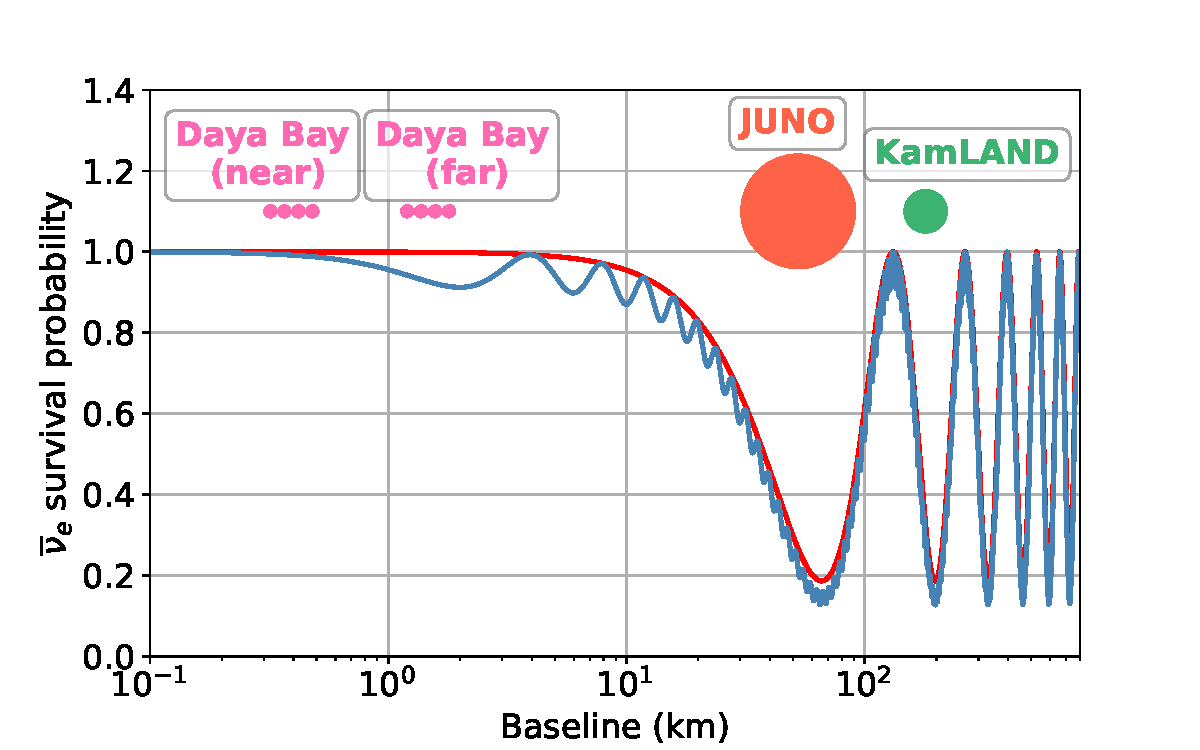
\includegraphics[width=0.9\linewidth]{Img/nuosc_juno.pdf}
\bicaption[反应堆反中微子存活概率随基线的变化]{反应堆反中微子在不同基线下的存活概率。红曲线为由 $\Delta m^2_{21}$ 驱动的慢振荡（太阳项），蓝曲线为包含由 $\Delta m^2_{3\ell}$ 驱动的快振荡在内的三味总存活概率。图中标示了 JUNO（橙色，基线约 52.5\,km，接近太阳振荡极大值）、大亚湾（粉色，近/远基线）和 KamLAND（绿色）的实验基线位置；图片来自文献\citep{abusleme2025measurementreactorneutrinooscillations}}{Reactor $\bar{\nu}_e$ survival probability as a function of baseline for a 4\,MeV antineutrino. The red curve shows the slow (solar) oscillation driven by $\Delta m^2_{21}$, while the blue curve shows the full three-flavor survival probability including the fast (atmospheric) oscillations driven by $\Delta m^2_{3\ell}$. Experimental baselines are indicated for JUNO (orange, 52.5\,km; near the solar-oscillation maximum), Daya Bay (pink, near/far detectors), and KamLAND (green). Taken from Ref\citep{abusleme2025measurementreactorneutrinooscillations}}
\label{fig:reactor_survival_baseline}
\end{figure}

如图~\ref{fig:reactor_survival_baseline} 所示，在不同基线条件下，短基线实验（例如大亚湾近/远站）主要观测由 $\Delta m^2_{31}$/$\Delta m^2_{32}$ 驱动的”快振荡”，其振荡极大值位于约 2\,km 附近；而中长基线实验（例如 JUNO）则位于由 $\Delta m^2_{21}$ 驱动的”慢振荡”极大值附近（约 65\,km），因此 JUNO 能在同一次能谱测量中同时对慢、快两类频率成分敏感。

在传播介质中，中微子除了自由传播相位外，还会与介质中的电子、中子发生相干的前向散射，从而在味基下引入额外的有效势项。对于电子中微子，除中性流外还存在带电流相互作用，产生有效势\cite{Wolfenstein1978,Mikheyev1985}
\begin{equation}
V_e=\sqrt{2}\,G_F N_e,
\label{eq:Ve-matter}
\end{equation}
其中 $G_F$ 为费米常数，$N_e$ 为电子数密度；而缪子与陶子中微子仅有中性流贡献，其在味基下产生的相位相同，可被整体去除。因此在味基下的有效哈密顿量中，电子味分量相对于其它味有一个附加的能量偏移，导致传播本征态（有效质量与有效混合角）偏离真空值。
在两味近似下，可以将物质效应的结果写成对混合角与质量平方差的重整化\cite{Wolfenstein1978Matter, Mikheyev1985Resonance}：
\begin{equation}
\tan(2\theta_m)=\frac{\Delta m^2\sin(2\theta)}
{\Delta m^2\cos(2\theta)-2\sqrt{2}\,G_FN_e E}\,,
\label{eq:tan-2theta-m}
\end{equation}
并且
\begin{equation}
(\Delta m^2_m)^2=\bigl(\Delta m^2\cos2\theta-2\sqrt{2}\,G_FN_eE\bigr)^2
+\bigl(\Delta m^2\sin2\theta\bigr)^2,
\label{eq:dm2m-squared}
\end{equation}
其中 $E$ 为中微子能量，$\theta_m$ 与 $\Delta m^2_m$ 分别为介质中的有效混合角和有效质量平方差。由此可见，当满足共振条件
\begin{equation}
2\sqrt{2}\,G_FN_e E = \Delta m^2\cos(2\theta)
\label{eq:msw-resonance}
\end{equation}
时，$\theta_m$ 接近 $45^\circ$ 并取得极大值——即所谓的 MSW 共振，此时味态转换被显著增强\cite{Mikheyev1985Resonance, Bethe1986Possible}。值得注意的是，共振条件对中微子与反中微子符号相反（因 $V_e$ 对反中微子取负），因此同一介质下中微子与反中微子的物质修正方向不同。

在三味振荡情形中，需对 $3\times3$ 的有效哈密顿量数值对角化以获得精确的物质修正\cite{Zaglauer1988Analytic}；一般而言，物质效应主要影响与太阳项（$\Delta m^2_{21}$）相关的低频分量，而对于快频项（由 $\Delta m^2_{3\ell}$ 驱动）影响较小。对于太阳中微子（穿越太阳高密度区域），MSW 效应产生的大幅增强是解释太阳中微子缺失的关键机制\cite{SNO2002Solar}；而对于穿过地壳传播的反应堆反中微子（基线为数十公里、能量在 MeV 量级），物质势 $V_e$ 的数值通常较小，仅作为微小却必要的修正被纳入精密拟合，以避免在高精度测量（如 JUNO 等）中产生系统偏差\cite{JUNO2016YellowBook, Khan2015Matter}。

\section{江门中微子实验}

JUNO 的首要物理目标是通过精确测量反应堆中微子能谱来确定中微子的质量顺序（正常层级或倒置层级）\cite{An2016_YellowBook}。根据设计，JUNO 在约 6 年运行后可在 $3$--$4\sigma$ 置信度上区分两种质量层级。同时，JUNO 将以亚百分比级的精度精准测量主要振荡参数，如 $\theta_{12}$、$\Delta m^2_{21}$ 和 $\Delta m^2_{31}$，从而进一步完善三味振荡模型\cite{Abusleme2022_Physics}。除反应堆中微子研究外，JUNO 还具备探测太阳中微子、地球（地幔）中微子和超新星中微子的能力，并可进行惰性中微子、质子衰变等新物理现象的探索\cite{An2016_YellowBook}。这些物理目标的实现将为中微子物理学的未来研究提供关键数据和启示。

\subsection{JUNO 的探测器结构与关键参数}

如图\ref{fig:juno_detector}所示，JUNO的核心部件是一个直径35.4米的有机玻璃球形中心探测器，内部装有约20,000吨液体闪烁体\cite{Abusleme2022_Detector}。该玻璃球被浸没在深44米、容积约3.5万吨的水切伦科夫池中，水池既屏蔽周围岩石的本底射线，又安装了光电倍增管作为水切伦科夫探测器，用于标记通过的宇宙射线μ子\cite{Abusleme2025}。中心有机玻璃球外壁均匀布置了约20000只20英寸光电倍增管和25600只3英寸光电倍增管，用于收集来自闪烁体的光信号，这一双量能器系统（Dual-calorimetry）能够有效提升动态范围与校准精度\cite{Abusleme2022_PMT}。为了进一步抑制宇宙μ子背景，在水池顶部还安装有塑料闪烁体顶层径迹探测器（Top Tracker），用于精确记录穿过探测器的μ子轨迹并作为μ子标记\cite{Grassmann2014_TT}。

\begin{figure}[htbp]
    \centering
    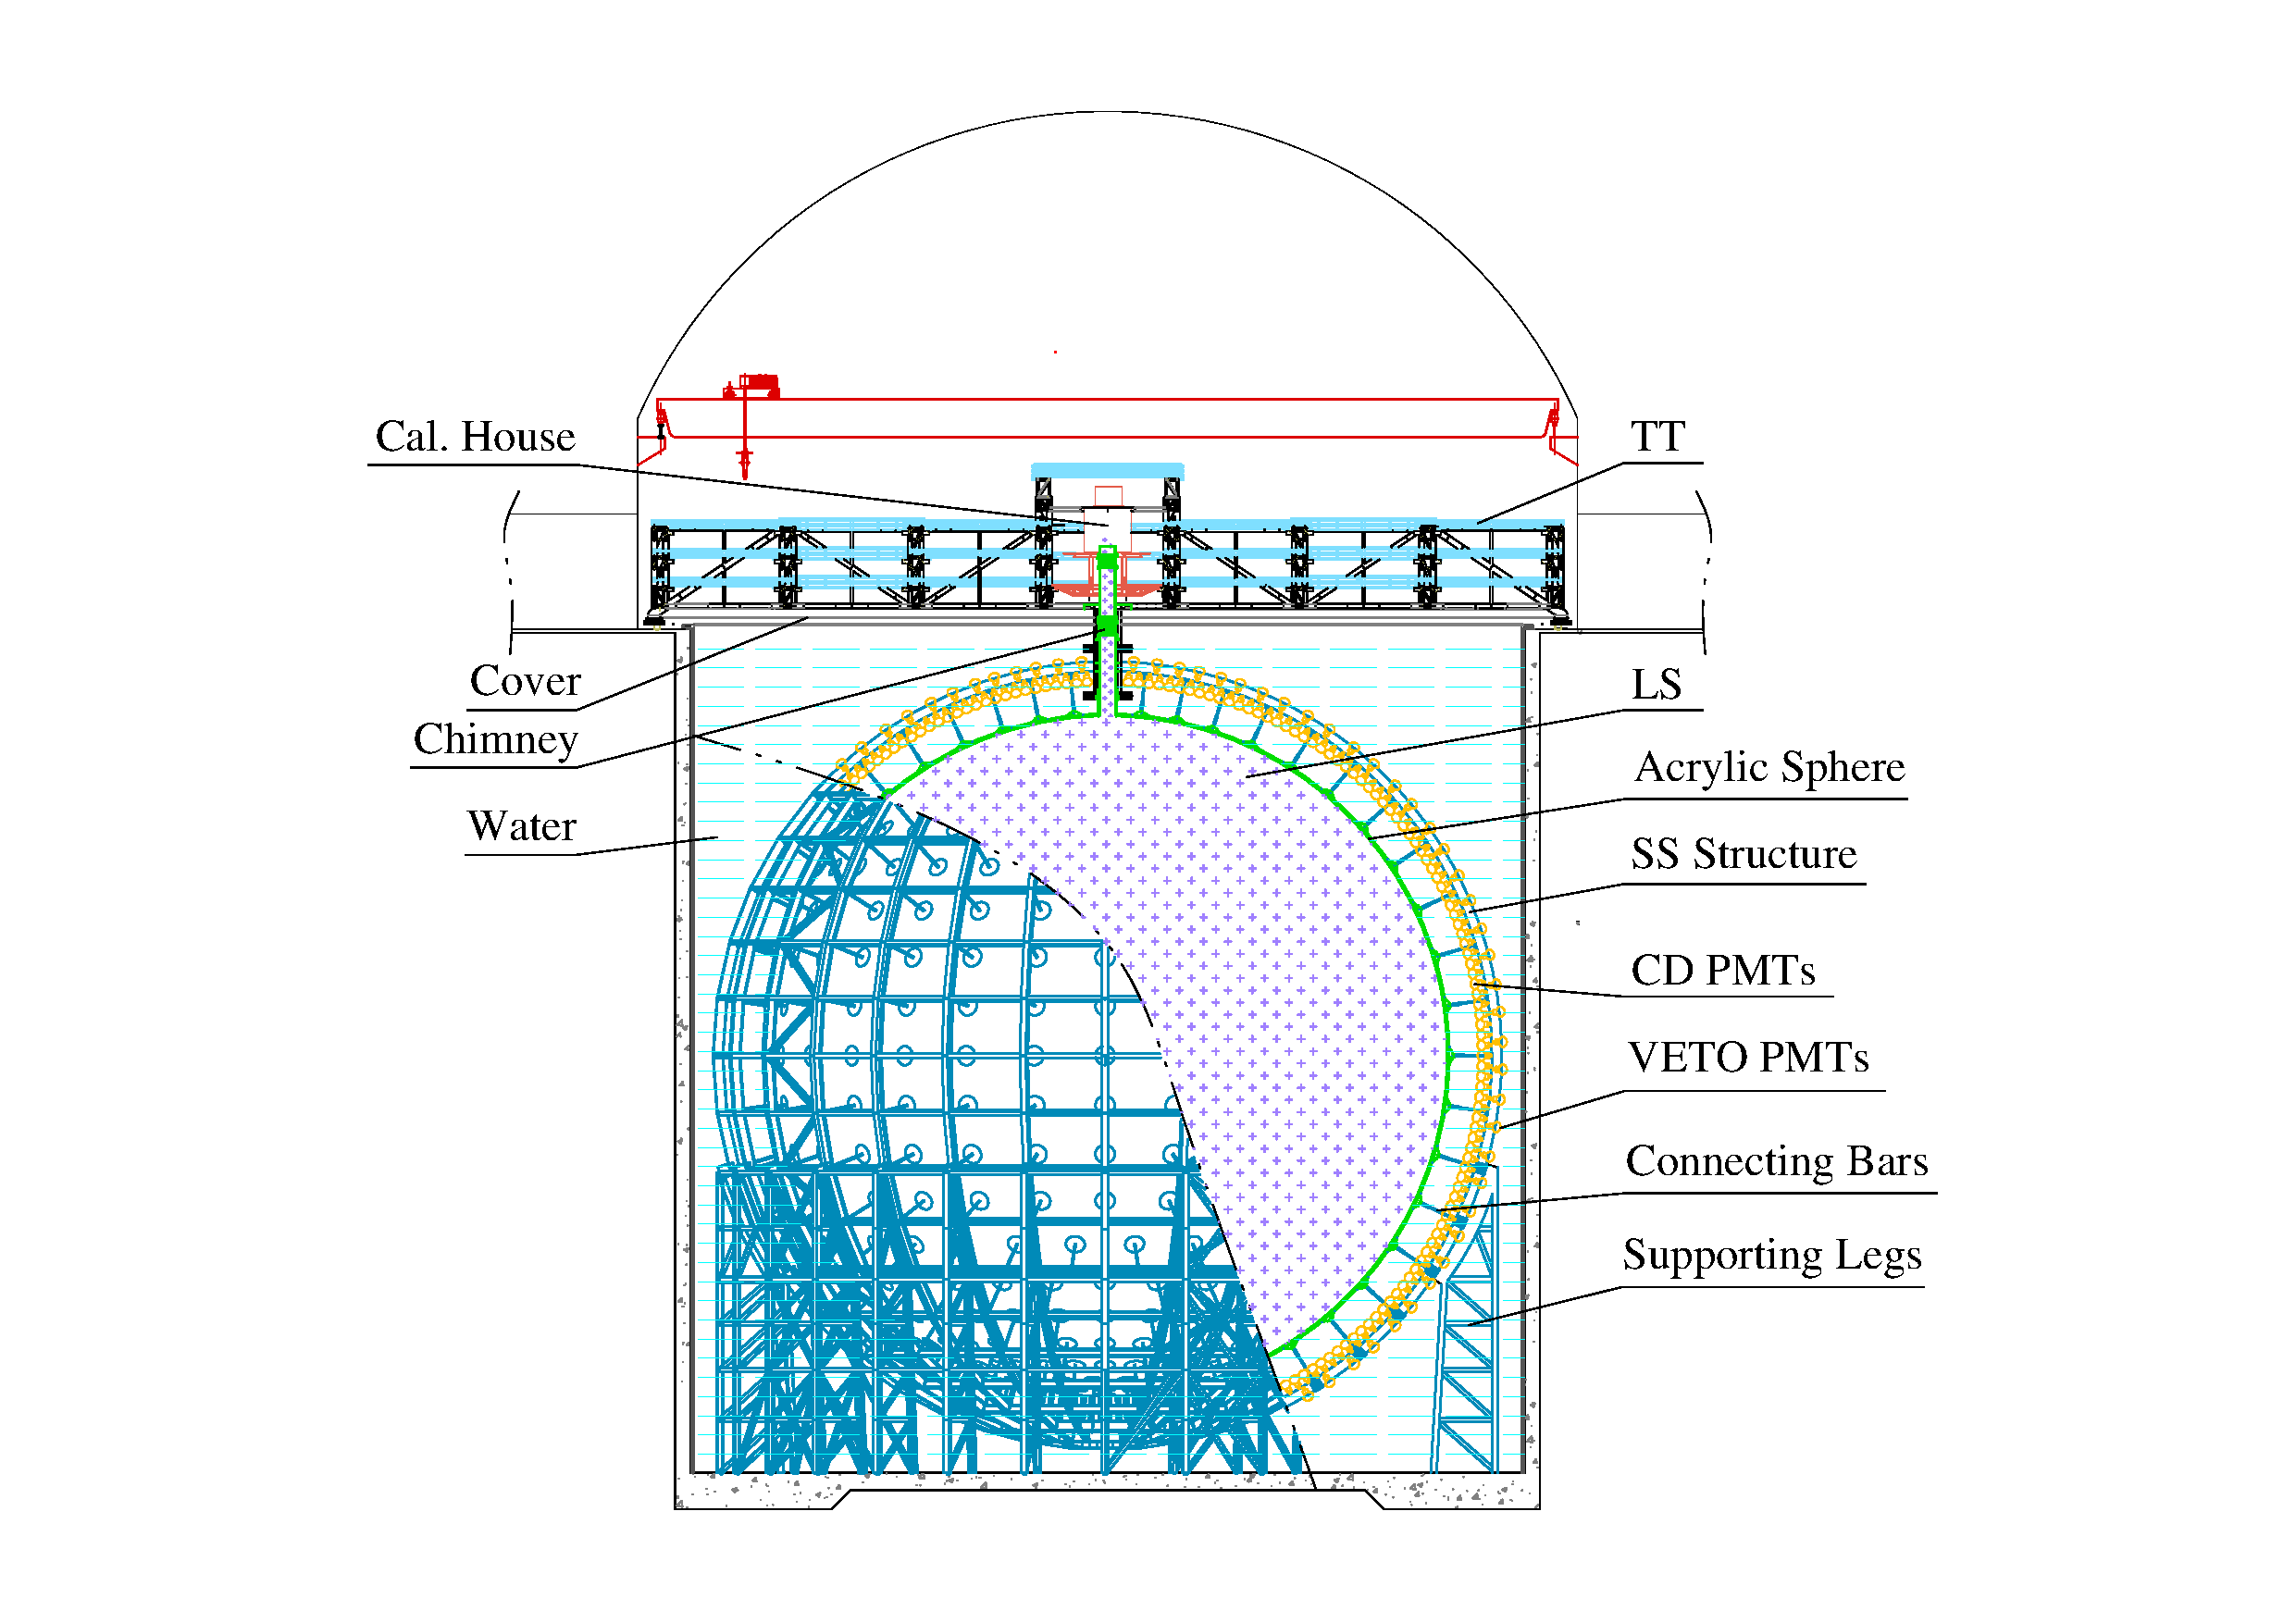
\includegraphics[width=0.9\linewidth]{Img/JUNO_Detector_Scheme.pdf}
    \bicaption[JUNO 探测器示意图]{JUNO 探测器示意图（图片来自文献\cite{Abusleme2025}）。}{Schematic view of the JUNO detector, taken from Ref.\cite{Abusleme2025}.}
    \label{fig:juno_detector}
\end{figure}

JUNO 探测器的关键指标之一是极高的能量分辨率。设计要求在 1~MeV 处达到约 3\% 的能量分辨率，相当于每 MeV 产生超过 1100 个探测光电子\cite{Abusleme2021_LS}。为此，探测器选用了高透射性的 LAB 基液体闪烁体，掺有荧光体 PPO 和波长转换剂 Bis-MSB\cite{Abusleme2021_LS}。探测器中安装了约 20000 只 20 英寸高效 PMT 和 25600 只 3 英寸 PMT，光电覆盖率约为 75\%，保证了足够的光收集效率以实现上述能量分辨率目标\cite{Abusleme2022_PMT}。

\subsection{JUNO 中的反应堆中微子}
JUNO 协作组于 2025 年底发布了首篇反应堆中微子振荡物理结果论文《First measurement of reactor neutrino oscillations at JUNO》\citep{abusleme2025measurementreactorneutrinooscillations}。该结果基于探测器完工后自 2025 年 8 月以来的 59.1 天数据，共选取到 2379 个逆 $\beta$ 衰变（IBD）中微子候选事件。通过对中微子快信号能谱的拟合分析，得到了真空三味振荡参数的高精度测量结果。

\begin{figure}[htbp]
\centering
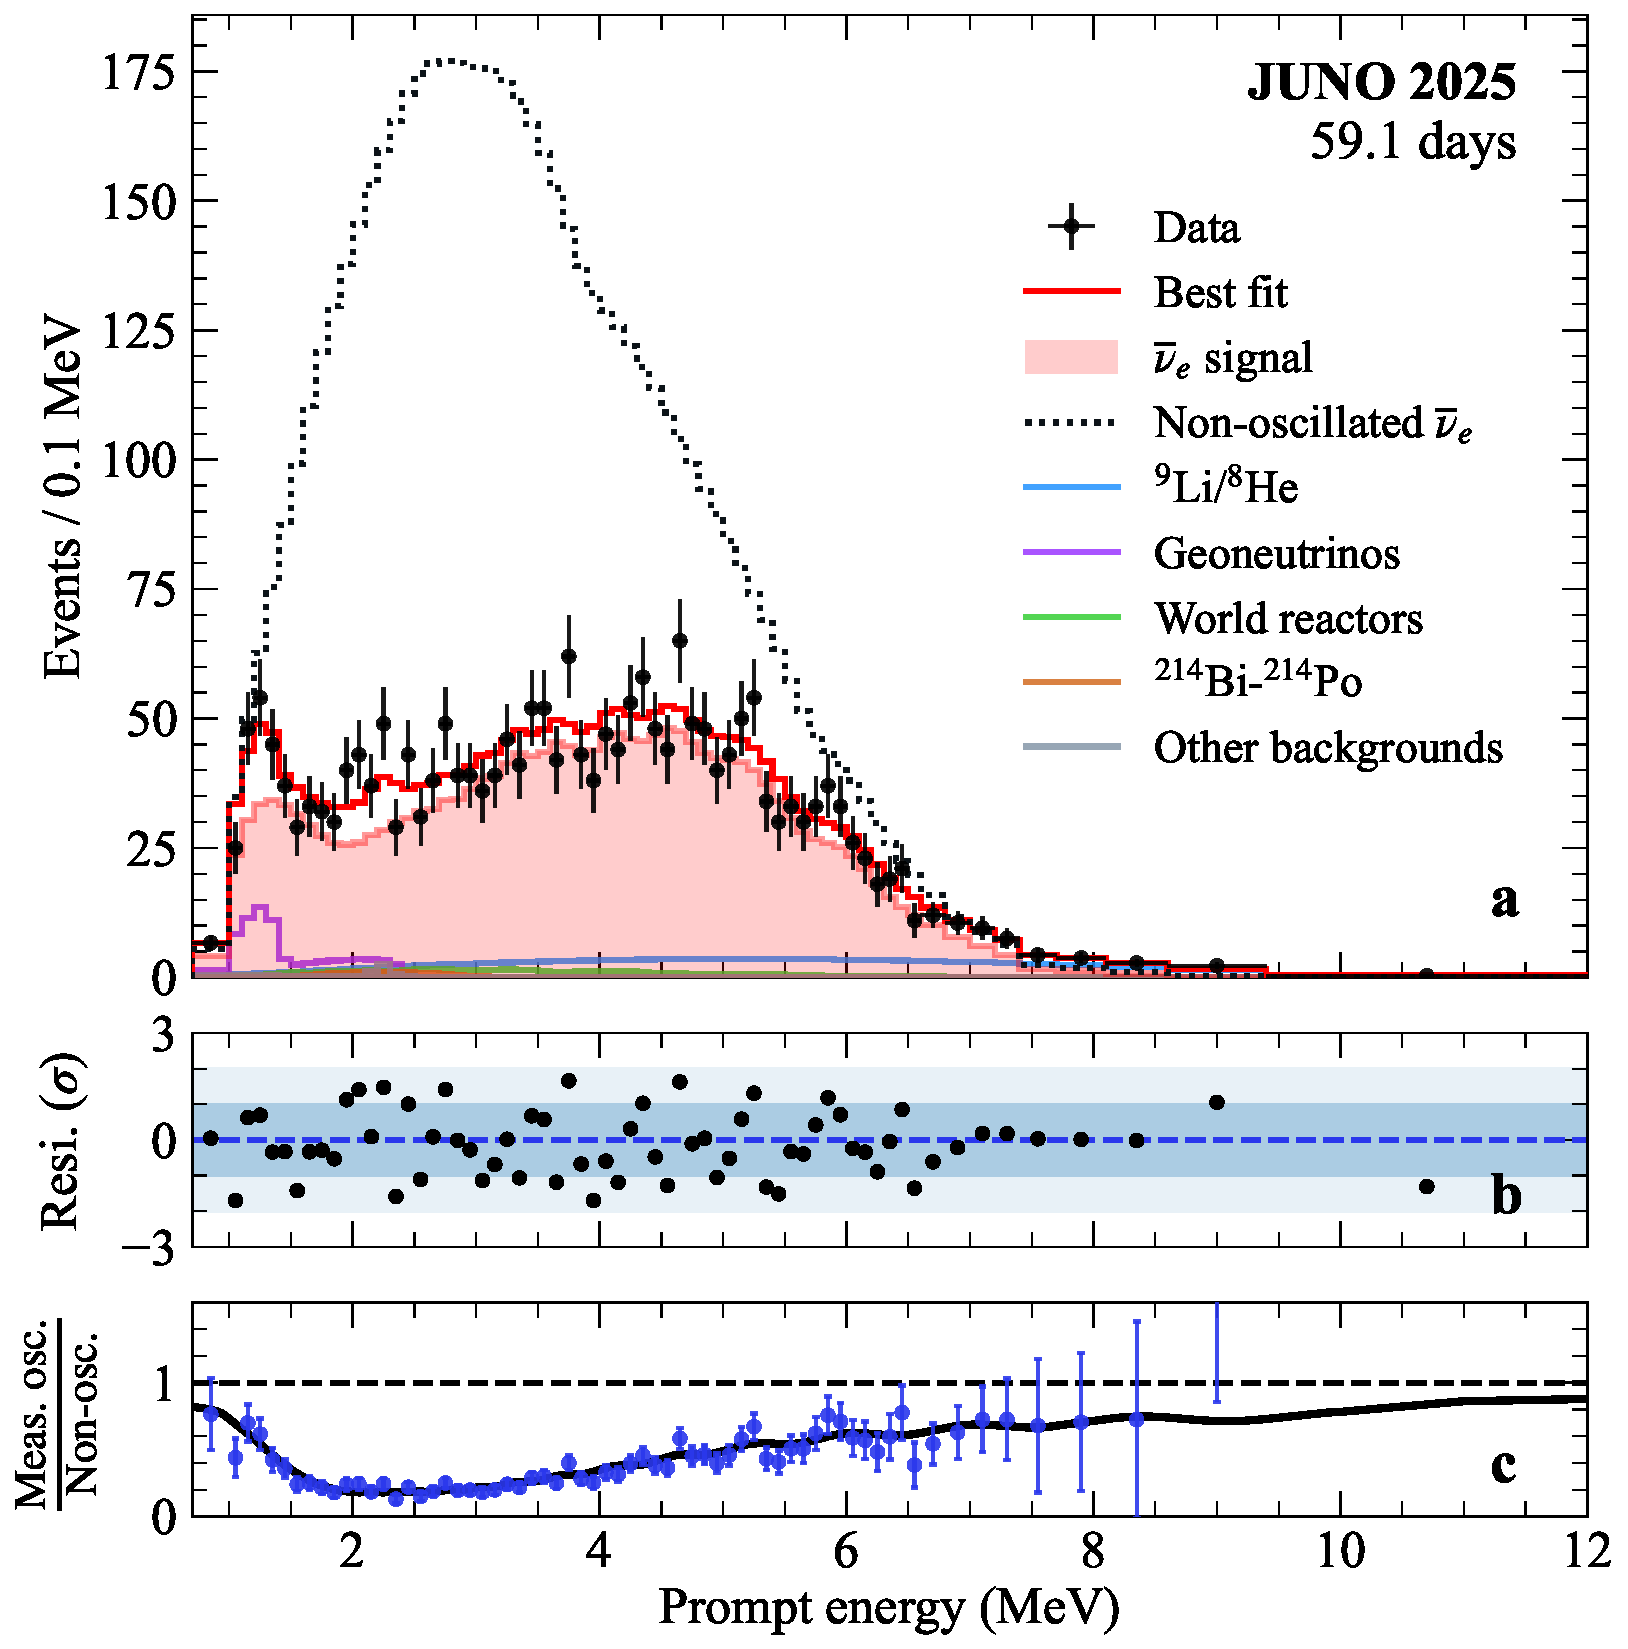
\includegraphics[width=0.9\linewidth]{Img/antineutrinoSpectrum.pdf}
\bicaption[测量能谱及拟合结果（JUNO 首篇物理分析结果，59.1 天数据）]{（a）黑点为经过事例挑选后的IBD 候选事例的测量值（带统计误差），红色实线为包含振荡效应的最佳拟合模型，红色阴影区为拟合出的反中微子信号分量。黑色虚线为若无振荡时的反应堆中微子预期谱。其他有色实线分别表示主要本底成分（例如宇宙线次级粒子$^9$Li/$^8$He、地球中微子、来自全球反应堆的中微子贡献、$^{214}$Bi--$^{214}$Po 等）。（b）数据与完整模型之间的残差及其一致性检验。（c）测得的振荡后谱与无振荡预测之比，显示能谱上的振荡形状特征。该图直接展示了在短期运行下 JUNO 对 IBD 能谱的重建能力与振荡信号的显著性（见文献\cite{abusleme2025measurementreactorneutrinooscillations}）。}{Prompt IBD energy spectrum and fit results (JUNO first physics measurement, 59.1 days). (a) Black points show the measured prompt energy distribution of selected IBD candidates with statistical error bars. The red curve indicates the best-fit oscillation model and the red shaded band denotes the fitted antineutrino signal component. The black dotted curve illustrates the non-oscillated reactor antineutrino expectation. Colored solid lines indicate major background contributions (e.g.\ cosmogenic $^9$Li/$^8$He, geoneutrinos, distant reactor background, $^{214}$Bi--$^{214}$Po, etc.). (b) Residuals quantifying the statistical consistency between data and the full model (in units of $\sigma$). (c) Ratio of the measured oscillated spectrum to the non-oscillated prediction, highlighting the spectral distortions induced by neutrino oscillations. Data are from JUNO Collaboration, First measurement of reactor neutrino oscillations at JUNO (59.1 days)\cite{abusleme2025measurementreactorneutrinooscillations}.}
\label{fig:juno_prompt_spectrum}
\end{figure}

图~\ref{fig:juno_prompt_spectrum} 展示了 JUNO 在首个 59.1 天采集期内的测量能谱、振荡最佳拟合与各类本底构成：测量谱与无振荡预测存在显著偏离，且谱形的能量依赖失真与三味振荡模型的拟合结果高度一致，直观证明了 JUNO 在能谱学测量和振荡参数约束上的能力。在假定正常质量序的情况下，测得 $\sin^2\theta_{12}=0.3092\pm0.0087$ 和 $\Delta m^2_{21}=(7.50\pm0.12)\times10^{-5}\,\mathrm{eV}^2$。

\begin{figure}[htbp]
\centering
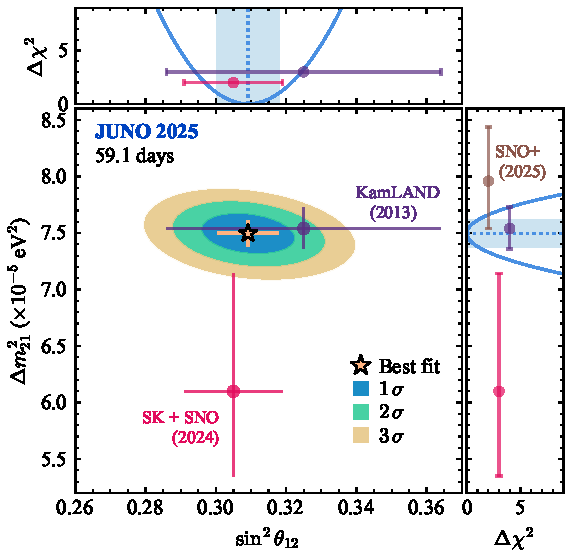
\includegraphics[width=0.9\linewidth]{Img/contour_sinsq12_dmsq21_withOtherExp.pdf}
\bicaption[太阳振荡参数约束（JUNO 59.1 天数据）]{基于 2025 年 59.1 天 JUNO 数据，通过对反应堆反中微子快信号能谱进行谱拟合得到的太阳振荡参数 $\sin^2\theta_{12}$ 与 $\Delta m_{21}^2$ 的约束结果。阴影椭圆区域分别对应 $1\sigma$、$2\sigma$ 和 $3\sigma$ 置信区间。上方（右侧）面板给出了对另一参数进行 profile 处理后得到的 $\sin^2\theta_{12}$（$\Delta m_{21}^2$）的一维 $\Delta\chi^2$ 分布。星号表示 JUNO 的最佳拟合值，误差棒表示对应的一维 $1\sigma$ 置信区间。同时给出了 KamLAND (2013)、SNO+ (2025) 以及 Super-Kamiokande 与 SNO 联合分析 (2024) 的结果以作比较。（见文献\cite{abusleme2025measurementreactorneutrinooscillations}）}{Constraints on the solar oscillation parameters $\sin^2\theta_{12}$ and $\Delta m_{21}^2$ obtained from a spectral fit to the measured prompt energy spectrum of reactor antineutrinos with 59.1 days of JUNO data (2025). The shaded elliptical regions correspond to the $1\sigma$, $2\sigma$, and $3\sigma$ confidence levels. The upper (right) panel shows the one-dimensional $\Delta\chi^2$ profile for $\sin^2\theta_{12}$ ($\Delta m_{21}^2$), where the other parameter is profiled. The star denotes the JUNO best-fit point, and the error bars indicate the corresponding $1\sigma$ intervals. Results from KamLAND (2013), SNO+ (2025), and the combined Super-Kamiokande (SK) + SNO (2024) analyses are shown for comparison.\cite{abusleme2025measurementreactorneutrinooscillations}}
\label{fig:juno_contour}
\end{figure}

图~\ref{fig:juno_contour} 表明这一测量精度比以往实验的组合结果提高了约 1.6 倍。JUNO 已能够通过反应堆反中微子能谱的精密测量，对太阳振荡参数 $\sin^2\theta_{12}$ 和 $\Delta m_{21}^2$ 给出具有竞争力的独立约束。系统误差方面，通过大量校准保证了能量标度不确定度约 $0.5\%$、正电子非线性约 $1\%$ 的约束；同时对来自宇宙射线次级粒子 $^9$Li/$^8$He 衰变等本底进行了严格抑制。实验结果为未来利用 JUNO 数据精确探究中微子质量顺序奠定了良好基础。

\subsection{JUNO 中的大气中微子}
JUNO 探测器还可观测大气中微子，其能量范围从100 MeV 到 10 GeV\citep{Abusleme2021}，通道覆盖从近地表至地球直径的路径长度（最长约 $1.3\times10^4\,\mathrm{km}$），对应广泛的 $L/E$ 范围（从几百到上万 km/GeV）。在几 GeV 以上能量区间内，JUNO 具有良好的能量和角分辨能力：对于 $E_\nu>3\,\mathrm{GeV}$ 的电子型大气中微子，能量重建优于 $6\%$，缪子型优于 $8\%$；其到达方向的角度分辨率在 $\sim10^\circ$ 量级。这些精度使 JUNO 能够通过对大气中微子在地球介质中出现的 MSW 效应进行研究，从而补充其主要的质量序测定方案。目前 JUNO 尚未发布大气中微子观测结果，但相关研究表明，利用大约 10 年的数据，大气中微子通道可提供约 $1.0$--$1.8\sigma$ 的质量序敏感度\citep{Zhang2023OscillationPhysicsPotential}。特别是将大气中微子结果与反应堆中微子结果结合分析，有望进一步增强整体灵敏度。

\begin{figure}[htbp]
\centering
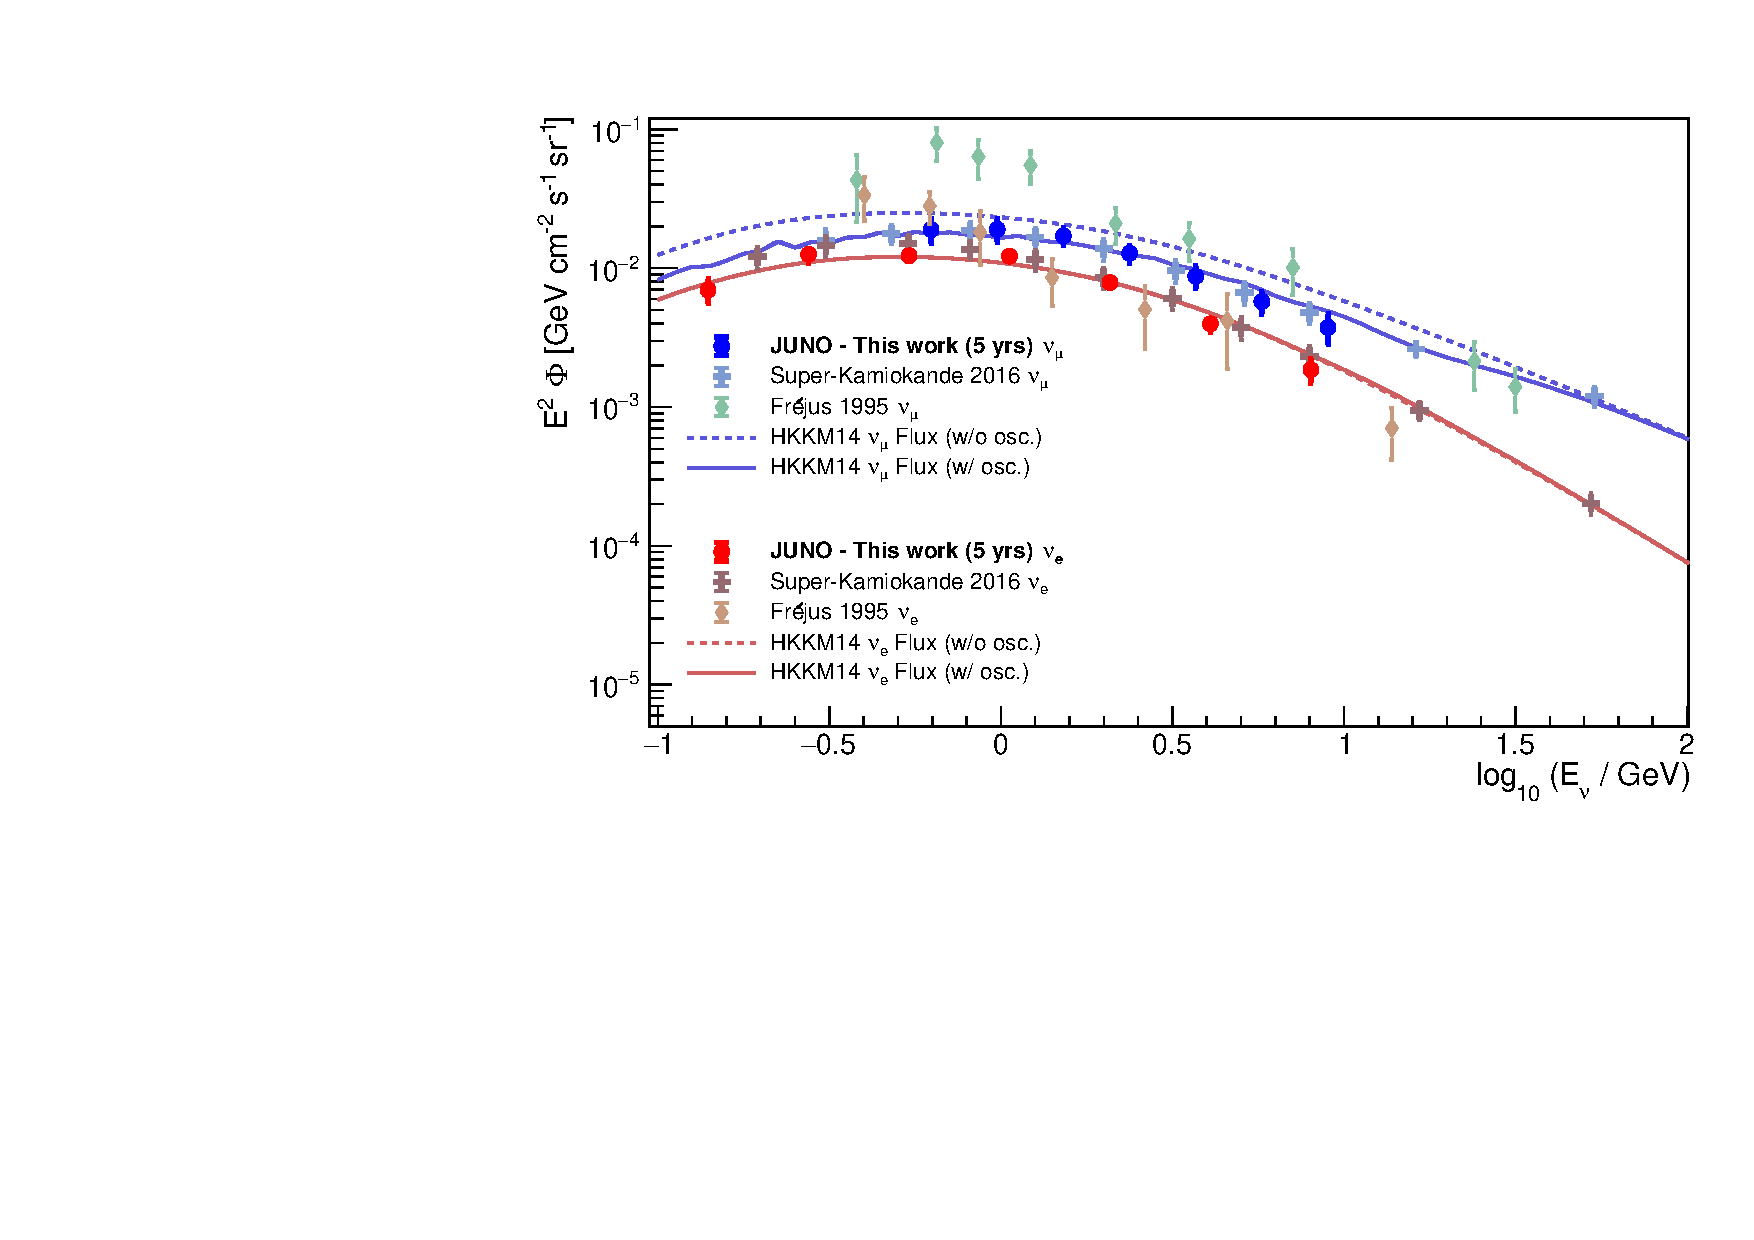
\includegraphics[width=0.9\linewidth]{Img/AtmoSpec_ALL_YB.pdf}
\bicaption[JUNO 对大气中微子能谱的灵敏度预期与现有实验结果比较]{JUNO 对大气中微子能谱的灵敏度预期与现有实验结果比较。图中给出了在 5 年运行时间下，JUNO 对大气中微子通量 $E^2\Phi$ 的预期测量结果（蓝色为 $\nu_\mu$，红色为 $\nu_e$），并与 Super-Kamiokande 2016 年测量结果以及 Fréjus 1995 年数据进行比较。同时给出了 Honda--Kajita--Kasahara--Midorikawa（HKKM14）大气中微子通量模型在考虑振荡（实线）和不考虑振荡（虚线）情况下的理论预期。横轴为中微子能量的对数刻度 $\log_{10}(E_\nu/\mathrm{GeV})$，纵轴为 $E^2\Phi$。可以看出，在 GeV 能区，振荡效应对 $\nu_\mu$ 通量产生显著压低，而 $\nu_e$ 通量则表现出相对增强或形状变化。JUNO 的测量精度在多 GeV 区间内具有良好的统计灵敏度，可用于检验大气中微子振荡模型并辅助质量顺序分析。该图来自文献\citep{Abusleme2025}}{Expected JUNO sensitivity to atmospheric neutrino flux compared with previous measurements and theoretical predictions. The figure shows the projected 5-year JUNO measurement of the atmospheric neutrino flux in terms of $E^2\Phi$ (blue points for $\nu_\mu$, red points for $\nu_e$). The results are compared with Super-Kamiokande 2016 measurements and Fréjus 1995 data. Theoretical predictions from the HKKM14 atmospheric neutrino flux model are shown both without oscillation (dashed lines) and with oscillation (solid lines). The horizontal axis represents $\log_{10}(E_\nu/\mathrm{GeV})$, and the vertical axis corresponds to $E^2\Phi$. The figure illustrates the suppression of $\nu_\mu$ flux due to oscillation effects in the GeV region, while modifications in the $\nu_e$ spectrum are also visible. JUNO demonstrates competitive sensitivity in the multi-GeV range, enabling further tests of atmospheric neutrino oscillations and complementary constraints on the neutrino mass ordering. Taken from Ref\citep{Abusleme2025}}
\label{fig:atmos_nu}
\end{figure}

如图~\ref{fig:atmos_nu} 所示，在 5 年运行时间下，JUNO 对 GeV 能区大气中微子通量的测量预期与 HKKM14 理论模型符合良好，并能够清晰分辨振荡与非振荡情形的差异，从而为质量顺序判定提供独立而互补的实验信息。

\subsection{JUNO 中的太阳中微子}
标准太阳模型预言太阳中微子主要来源于 pp 链和 CNO 循环反应，其能谱分布如图~\ref{fig:solar_nu_spectrum} 所示。

\begin{figure}[htbp]
\centering
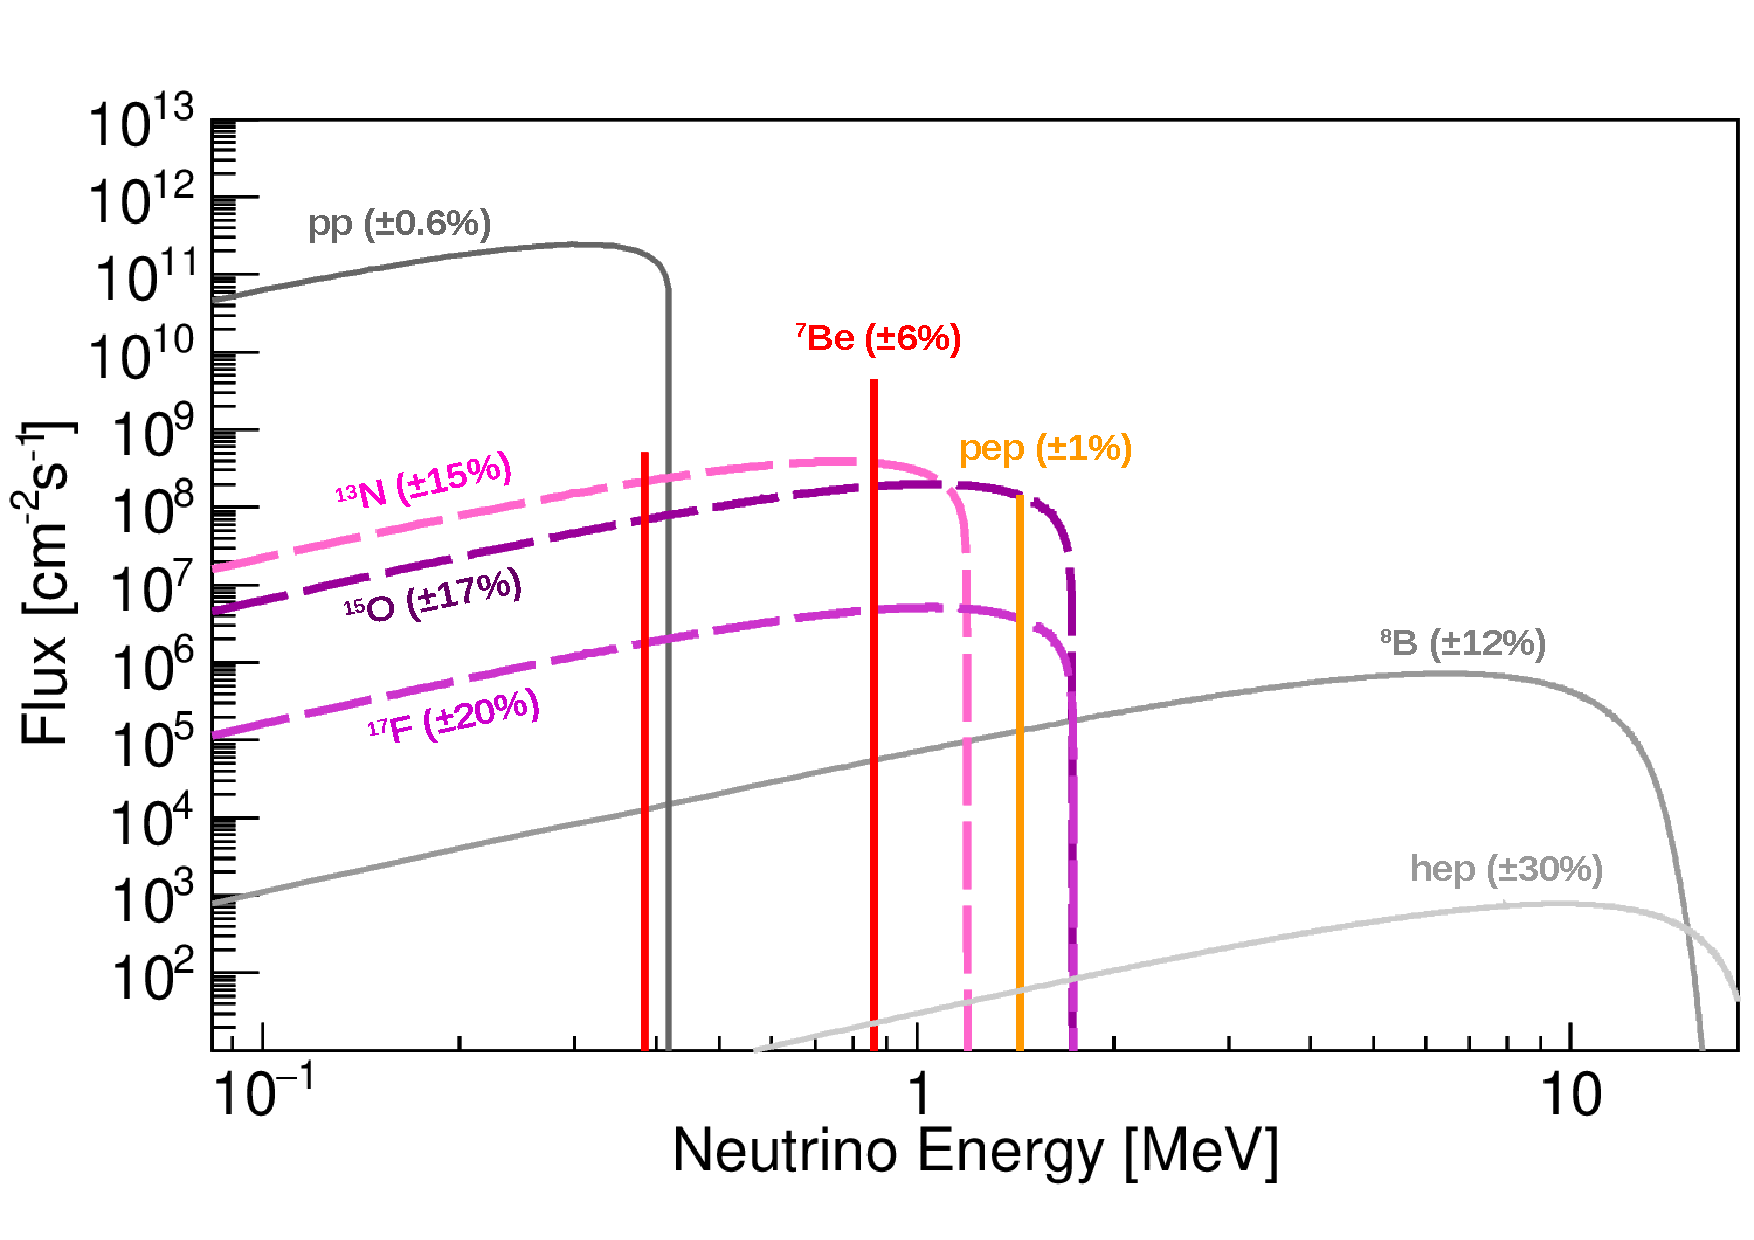
\includegraphics[width=0.9\linewidth]{Img/Fig2_v5.pdf}
\bicaption[太阳中微子能谱及理论通量预测]{太阳中微子能谱及理论通量预测。图中给出了标准太阳模型（Standard Solar Model, SSM）预测的各类太阳中微子通量随能量变化关系，包括 pp、$^7$Be、pep、$^8$B、hep 以及 CNO 循环产生的 $^{13}$N、$^{15}$O、$^{17}$F 中微子。不同曲线对应不同反应来源，括号中标注为理论通量的不确定度。红色和橙色竖线分别标示了 JUNO 对 $^7$Be 和 pep 单能谱太阳中微子的主要灵敏能区。该图展示了低能 pp 与 $^7$Be 中微子在太阳中微子总通量中的主导地位，以及高能 $^8$B 与 hep 中微子在高能区的重要贡献。图片来自文献\citep{Abusleme_2023}}{Solar neutrino fluxes predicted by the Standard Solar Model (SSM). The figure shows the theoretical solar neutrino flux as a function of neutrino energy for different components, including pp, $^7$Be, pep, $^8$B, hep, and CNO-cycle neutrinos ($^{13}$N, $^{15}$O, $^{17}$F). The quoted percentages indicate the theoretical uncertainties of each flux component. The red and orange vertical lines indicate the primary sensitivity regions of JUNO for monoenergetic $^7$Be and pep neutrinos. The figure highlights the dominance of pp and $^7$Be neutrinos in the low-energy region and the contribution of $^8$B and hep neutrinos at higher energies.Taken from Ref\citep{Abusleme_2023}}
\label{fig:solar_nu_spectrum}
\end{figure}

低能区（$E_\nu<2\,\mathrm{MeV}$）主要由 pp、$^7$Be 和 pep 中微子主导，其中 $^7$Be 为单能谱中微子，在约 $0.86\,\mathrm{MeV}$ 处形成明显特征信号；而高能区则由 $^8$B 与 hep 中微子贡献。JUNO 由于具有大体积液体闪烁体和优异的能量分辨率（约 $3\%$ @ $1\,\mathrm{MeV}$），在抑制放射性本底后，有望实现对 $^7$Be（$862\,\mathrm{keV}$）、pep（$1.44\,\mathrm{MeV}$）和 CNO 循环（$1$--$2\,\mathrm{MeV}$）中微子的精确测量，从而进一步检验太阳模型并研究低能区的物质增强振荡效应（MSW-LMA 区域）。研究表明，在达到与 Borexino 相当的极低本底放射纯度水平时，JUNO 有望在绝大多数情况下优于现有对这三种中微子通量的精密测量\citep{Abusleme_2023}。目前 Borexino 已分别以 $2.7\%$ 精度测出 $^7$Be 中微子通量，并首次 $5\sigma$ 检出 pep 中微子和 CNO 中微子的存在，但其探测器规模仅 100 吨量级。相比之下，JUNO 拥有 20 千吨的大体积液体闪烁体，统计灵敏度显著更高；但要实现同样水平的本底抑制，需要将 $^{238}$U、$^{232}$Th 及 $^{210}$Bi/$^{210}$Po 等内在放射性控制到极低水平。若材料纯化和屏蔽达标，模拟表明 JUNO 可在 1 年内记录上百至数百个 $^7$Be/pep 事件，并在 CNO 中微子通量的测量上取得突破\citep{Abusleme_2023}。JUNO 对太阳中微子的系统亮点在于大体积带来的统计优势和极高能量分辨，但挑战在于非信号本底（如 $^{85}$Kr、$^{11}$C 等）的控制。因此，JUNO 将重点优化极低本底条件下的事例挑选和能谱拟合方法，以期达到或超越 Borexino 在 ppm 级别本底控制的灵敏度。



\subsection{JUNO 中的超新星中微子}
JUNO 对银河系内超新星的中微子爆发具极强响应能力。根据模型预估，一场典型的核心塌缩超新星爆发将在约 10 秒内产生大量低能中微子信号：IBD 通道（$\bar\nu_e+p\to e^++n$）可记录约 5000 个事件，弹性散射通道（中微子与电子散射）记录约 300 个事件，而中微子与质子散射通道可记录 $\sim2000$ 个事件\citep{Lombardo2023SupernovaJUNO}。

\begin{figure}[htbp]
\centering
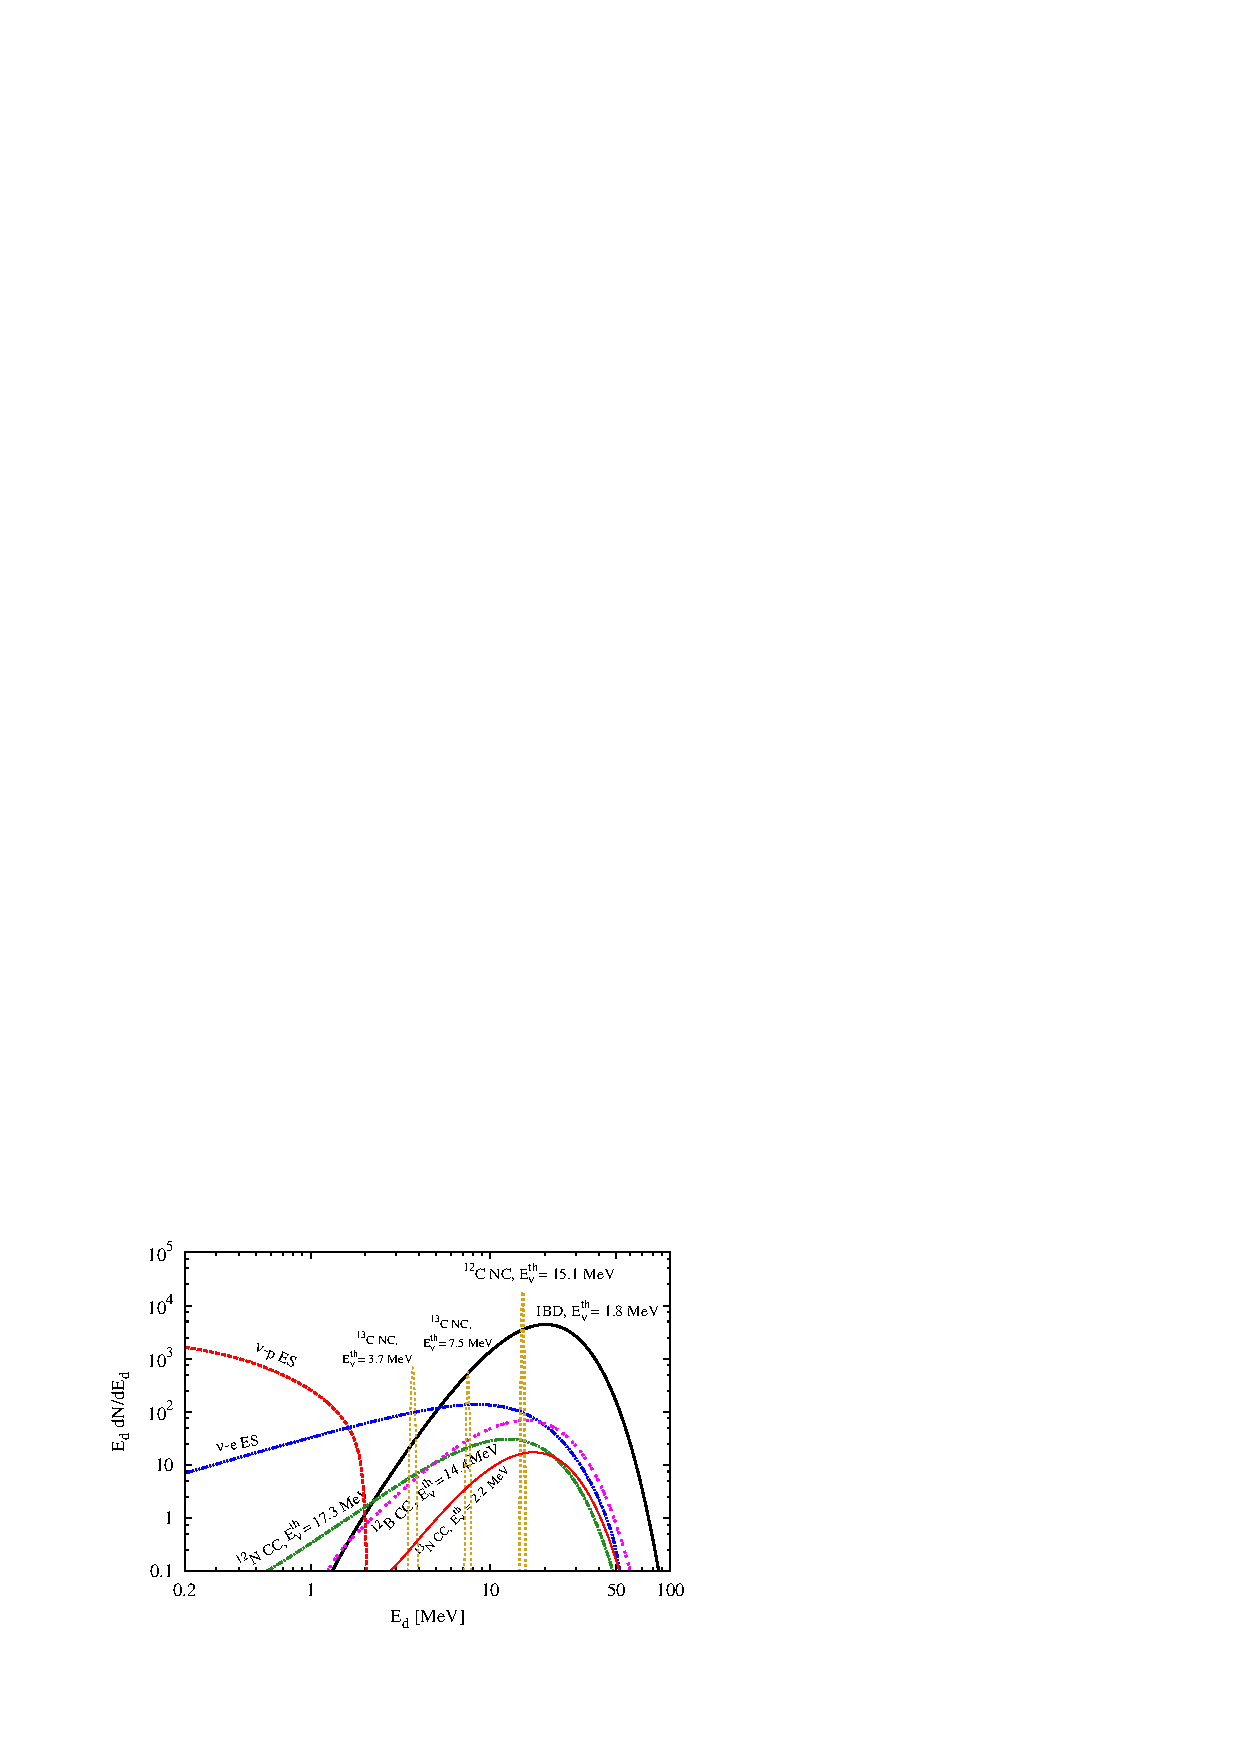
\includegraphics[width=0.9\linewidth]{Img/SNspectra.pdf}
\bicaption[JUNO 探测器中不同超新星中微子相互作用通道的沉积能量分布]{JUNO 探测器中不同超新星中微子相互作用通道的沉积能量分布。图中给出了在一次典型银河系核心坍缩超新星爆发条件下，JUNO 探测器内不同反应通道的可观测沉积能量 $E_{\mathrm{d}}$ 分布，包括反 $\beta$ 衰变（IBD，$\bar{\nu}_e + p \to e^+ + n$）、电子弹性散射（$\nu$--e ES）、质子弹性散射（$\nu$--p ES）、以及在 $^{12}$C 和 $^{13}$C 上的带电流（CC）与中性流（NC）反应。图中同时标注了各反应的能量阈值 $E_\nu^{\mathrm{th}}$。可以看到，IBD 通道在数十 MeV 能区贡献最大，是 JUNO 探测超新星 $\bar{\nu}_e$ 的主导通道；图片来自文献\citep{Abusleme2025}}{Deposited energy distributions of different supernova neutrino interaction channels in JUNO. The figure shows the visible deposited energy $E_{\mathrm{d}}$ spectra in JUNO for various interaction channels induced by a typical core-collapse supernova neutrino burst. These include inverse beta decay (IBD, $\bar{\nu}_e + p \to e^+ + n$), neutrino--electron elastic scattering ($\nu$--e ES), neutrino--proton elastic scattering ($\nu$--p ES), and charged-current (CC) and neutral-current (NC) interactions on $^{12}$C and $^{13}$C. The neutrino energy thresholds $E_\nu^{\mathrm{th}}$ for each reaction are indicated. The IBD channel dominates in the tens-of-MeV region and provides JUNO's primary sensitivity to $\bar{\nu}_e$. Taken from Ref\citep{Abusleme2025}}
\label{fig:supernova_channels}
\end{figure}

如图~\ref{fig:supernova_channels} 所示，反 $\beta$ 衰变通道在数十 MeV 能区具有最高统计量，是 JUNO 探测超新星 $\bar{\nu}_e$ 的核心通道；同时，$^{12}$C 与 $^{13}$C 上的中性流反应以及弹性散射通道为研究全味道中微子谱及爆发动力学过程提供了重要补充信息。此外，中微子与碳原子核的相互作用（含带电流和中性流反应）也会贡献数百个事件。如此高的统计量可让 JUNO 对超新星信号进行时域和能谱的精细测量，检验超新星核心坍缩模型\citep{Li2020Prospects}。JUNO 探测器还可参与国际超新星预警网络（SNEWS），在探测到信号时提供爆发的预警定位。研究估计，当观测到约 5000 个 IBD 事件时，JUNO 对超新星方向的定位精度可达到约 $9^\circ$ 不确定度\citep{Lorenz2016NeutrinoAstroJUNO}，足以配合光学望远镜迅速搜索可能的爆发源。

\subsection{JUNO 中的地球中微子}
JUNO 设计同样适用于探测来自地球内部放射性元素衰变产生的地球中微子（主要来源于 $^{238}$U 和 $^{232}$Th 衰变链）。利用与反应堆中微子相同的 IBD 反应，JUNO 每年预计可记录约 400 个地球中微子事件\citep{Ludhova2023JUNOStatus}。这一统计量远超当前 Borexino 和神冈两个实验多年来的累计结果（Borexino 约 50 个/年，神冈约 100 个/年）。如此高的事件率意味着 JUNO 将很快达到现有实验的灵敏度，并进一步精确测定地球中微子通量\citep{Ludhova2023JUNOStatus}。地球中微子的测量在地质学上意义重大：它为估算地幔与岩石圈中放射性元素丰度提供了独一无二的探针，可进一步推算地球的放射生热总量。JUNO 的测量还可以对 $^{232}$Th/$^{238}$U 比值进行约束，从而帮助验证地球化学模型对深部地热源贡献的预测\citep{Li2026Prospects}。

\begin{figure}[htbp]
\centering
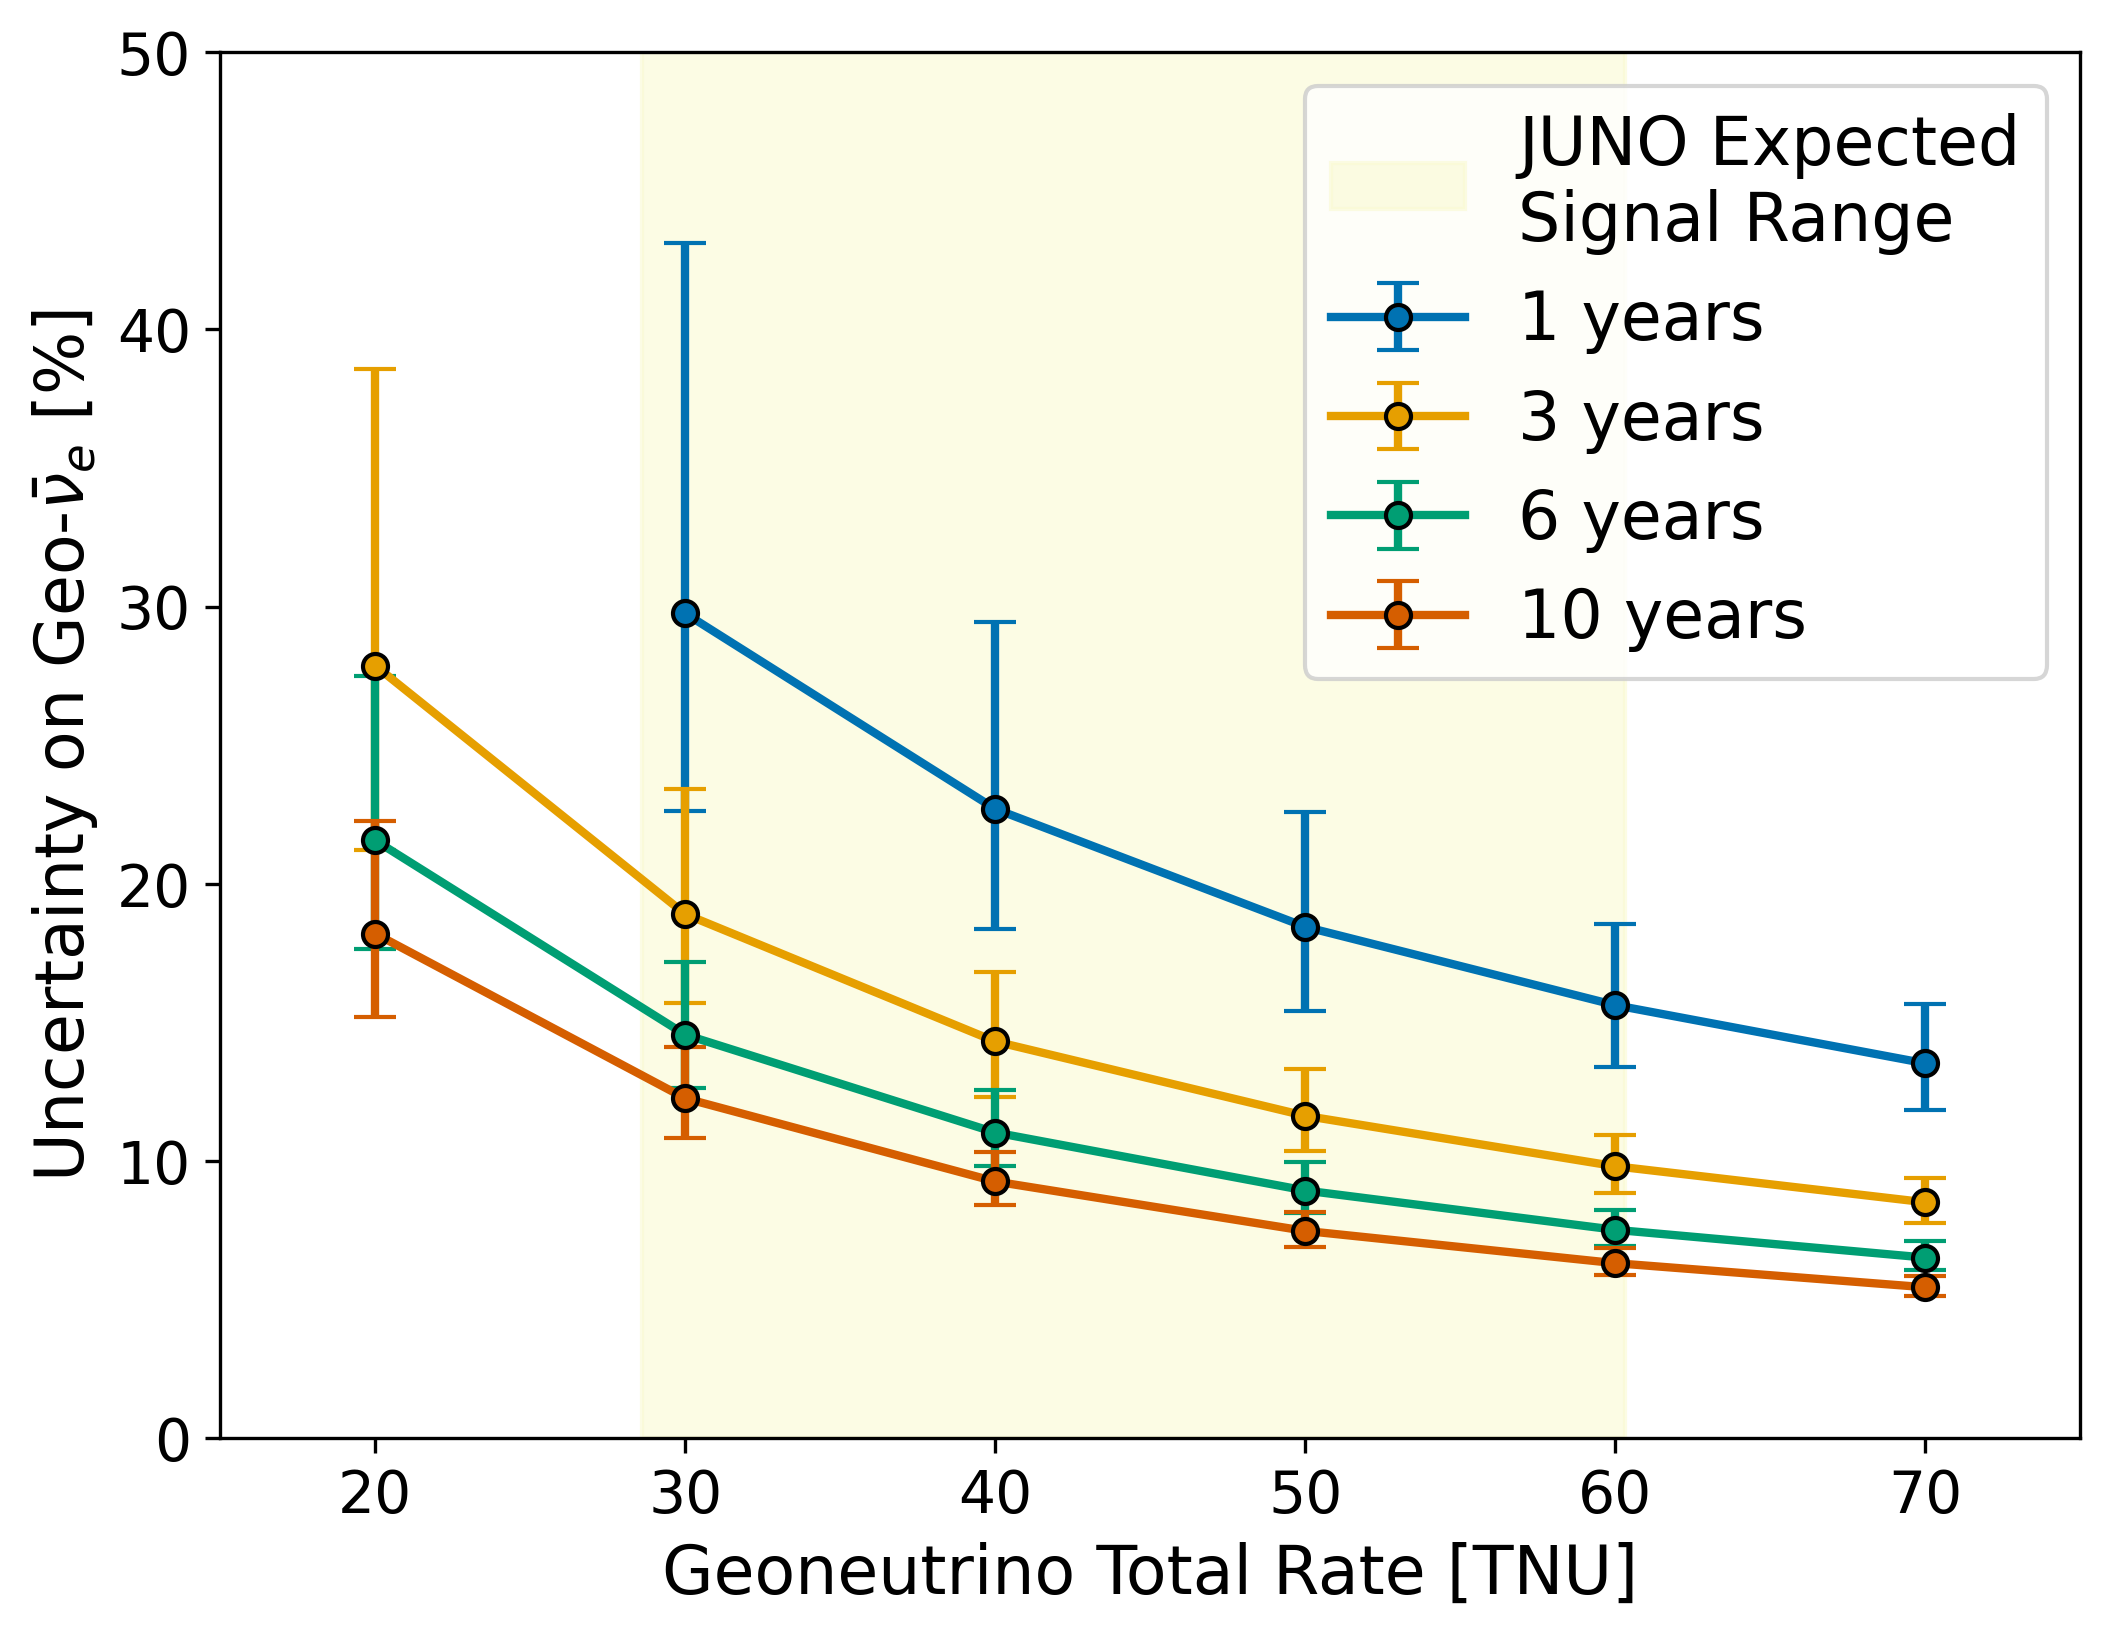
\includegraphics[width=0.9\linewidth]{Img/ScanGeo.png}
\bicaption[JUNO 对地球中微子总信号的预期测量精度]{JUNO 对地球中微子总信号的预期测量精度。图中给出了在假设 Th/U 比为球粒陨石比例条件下，JUNO 对地球中微子总信号（单位：TNU）的预期相对不确定度随总信号强度变化关系。蓝色、橙色、绿色和红色曲线分别对应 1 年、3 年、6 年和 10 年运行时间的灵敏度预期。纵轴表示对地球中微子总信号的相对不确定度（\%），横轴为地球中微子总事例率。黄色阴影区域表示不同 BSE（Bulk Silicate Earth）模型及岩石圈贡献预测所给出的 $1\sigma$ 信号区间。结果表明，随着运行时间增加，统计不确定度显著降低，在 10 年运行条件下可实现约 $5\%$--$7\%$ 量级的测量精度，从而对地球内部放射性元素分布模型形成重要约束。图片来自文献\citep{Li2026Prospects}}{Expected JUNO sensitivity to the total geoneutrino signal. The figure shows the projected relative uncertainty on the total geoneutrino signal (in TNU), assuming a fixed chondritic Th/U ratio, as a function of the total geoneutrino rate. The blue, orange, green, and red curves correspond to exposures of 1, 3, 6, and 10 years, respectively. The vertical yellow shaded region indicates the $1\sigma$ range of predicted signals from various Bulk Silicate Earth (BSE) models, including different assumptions for the lithospheric contribution. The results demonstrate that the measurement precision improves significantly with increased exposure, reaching approximately $5\%$--$7\%$ uncertainty after 10 years of operation, enabling strong constraints on Earth's radiogenic heat production models.Taken from Ref\citep{Li2026Prospects}}
\label{fig:geo_nu}
\end{figure}

如图~\ref{fig:geo_nu} 所示，随着运行时间的增加，JUNO 对地球中微子总信号的测量不确定度将显著降低，在 10 年运行条件下有望达到约 $5\%$ 量级的精度，从而有效区分不同 BSE 模型并约束地球内部放射性元素的分布。

\section{论文内容与结构}

本文围绕反应堆中微子振荡测量中的若干关键科学问题展开研究。针对低统计量条件下拟合偏差、联合分析中的模型依赖问题、振荡参数简并以及置信区间覆盖失效等现象，系统研究了合理的能谱分 bin 策略与Feldman-Cousins方法，并在此基础上提出了高性能的前向折叠反应堆中微子能谱计算与拟合框架，对基于大量 toy Monte Carlo 的分析流程进行了加速优化，以保证在有限算力条件下研究工作的可行性与精确性。

全文结构安排如下：

\textbf{第一章 引言}\\
本章首先回顾中微子的发现与基本物理性质，介绍中微子在标准模型中的地位及其可能的新物理含义，并系统梳理中微子振荡理论的基本框架。随后介绍江门中微子实验（JUNO）的探测结构、关键参数与主要物理目标，包括反应堆中微子、大气中微子、太阳中微子、超新星中微子以及地球中微子的探测研究，最后给出全文结构概述。

\textbf{第二章 中微子振荡分析方法（Oscillation Analysis Methods）}\\
本章系统介绍反应堆中微子的探测原理与能谱预测方法，包括核反应堆反中微子通量计算、沉积能量谱与重建能量谱构建，以及统计拟合方法的基本框架,同时介绍了前向折叠反应堆中微子拟合框架的能谱生成张量化表示。重点讨论低统计量条件下统计假设的适用性问题，分析 Wilks 定理的适用范围与局限性，并为后续引入 Feldman–Cousins 方法奠定理论基础。

\textbf{第三章 反应堆拟合程序的加速（Acceleration Strategies）}\\
由于分 bin 策略优化与 Feldman–Cousins 覆盖性研究均依赖海量 toy MC 实验，本章围绕拟合算法的性能优化展开研究。首先分析问题规模与性能瓶颈，随后从缓存技术、微分截面矩阵稀疏存储方式以及响应矩阵分块计算优化等方面实现算法加速，并对不同 bin 设置下的耗时影响进行系统测试，为大规模伪实验研究提供计算保障。

\textbf{第四章 JUNO 实验能谱分 bin 策略研究}\\
本章针对低统计量条件下高斯近似失效的问题，研究重建能谱的合理分 bin 策略，量化分 bin 选择对振荡参数偏差与精度的影响。进一步讨论 JUNO 与大亚湾（Daya Bay）联合分析中，由于两实验能量分辨率差异导致的 Wiggle 结构问题，指出若分 bin 过细可能超过 Daya Bay 实验约束能力，从而引入模型依赖系统误差。本章通过 Toy MC 系统研究不同分 bin 方案对结果稳定性与精度的影响，并提出合理优化方案。

\textbf{第五章 Feldman–Cousins 方法详述}\\
针对低统计量下振荡参数（特别是 $\Delta m^2_{31}$）存在简并、多极小值及不连续置信区间的问题，本章系统介绍 Feldman–Cousins 方法的基本思想与实现流程。通过大量 toy MC 实验研究 Wilks 近似的失效情况，验证 Feldman–Cousins 方法的覆盖性质，并分析临界值对扫描区间与参数空间的依赖性，确保置信区间具有正确的统计覆盖率。

\textbf{第六章 总结与展望}\\
本章对全文的研究工作进行系统总结，并对未来方向进行展望。总结部分回顾了基于张量化思想构建的高性能前向折叠反应堆中微子能谱计算与拟合框架、针对低统计量条件下重建能谱分 bin 与 JUNO--大亚湾联合分析中反应堆能谱分段（segment）策略的系统研究、以及基于 Feldman--Cousins 方法的频率学覆盖性检验三项主要成果，并阐述其对 JUNO 首篇物理结果论文所采用的统计方法与分段方案的实际贡献。展望部分讨论 JUNO 随统计量累积后 $\Delta m^2_{31}$ 精确测量所面临的非渐近统计挑战、JUNO 与近点高分辨率探测器 TAO 联合分析对实现近模型独立测量的关键作用，以及在质量序判定、无中微子双贝塔衰变（$0\nu\beta\beta$）与 CP 破坏相位测定等国际中微子物理前沿方向上的研究前景。

\section{本章小结}

本章系统回顾了中微子物理的研究脉络与基本物理性质：从 $\beta$ 衰变能量连续谱之谜与泡利中微子假说出发，梳理了三代中微子的相继发现以及宇称破缺、二分量中微子理论与中微子左旋性的确立；进而讨论了中微子在标准模型中的地位，阐述了为解释非零中微子质量而引入的跷跷板机制等新物理图像，并系统介绍了 PMNS 混合矩阵、真空三味振荡概率以及 MSW 物质效应等振荡理论要素，给出了后续分析所依赖的反应堆反中微子存活概率表达式。

本章还介绍了江门中微子实验（JUNO）的探测器结构与关键性能指标——包括 20\,kt 液体闪烁体中心探测器、水切伦科夫屏蔽以及 20 英寸与 3 英寸 PMT 构成的双量能器系统，达到约 3\% @ 1\,MeV 的能量分辨率——并概述了 JUNO 对反应堆中微子、大气中微子、太阳中微子、超新星中微子和地球中微子等多种中微子源的探测能力及主要物理目标。2025 年底发布的 JUNO 首篇物理结果已将太阳振荡参数 $\sin^2\theta_{12}$ 与 $\Delta m^2_{21}$ 的测量精度相对全球既有结果提升约 1.6 倍，标志着中微子物理由"发现时代"进入"高精度测量时代"。这些物理背景与实验概况为后续章节围绕反应堆中微子振荡测量所展开的能谱预测框架构建、分 bin 与分段策略研究以及 Feldman--Cousins 覆盖性检验等方法学工作奠定了物理基础。


% 可选择插入结构图示意
%=====================================================================
\chapter{中微子振荡分析方法（Oscillation Analysis Methods）}
%=====================================================================
反应堆中微子实验的核心目标是通过精确测量反中微子能谱的精细结构来提取振荡参数，并进一步判定中微子质量顺序。对于如 JUNO 这类中基线实验而言，振荡信号体现在重建能谱中的振荡起伏结构上。要可靠解析这些微小结构，必须对“从反应堆到重建谱”的完整物理与统计链条进行统一、精确且可计算的建模。任何一个环节的近似处理或数值误差，都可能在参数提取中放大为系统偏差。因此，建立一个物理自洽、并适用于大规模统计检验的分析框架，是开展后续灵敏度与覆盖率研究的基础。

本章实现了从反应堆出射谱到探测器重建能量谱的张量化谱生成链，将其分解为四个明确的矩阵/张量层次：反应堆中微子能谱（source spectrum），IBD 微分散射截面矩阵（cross-section tensor），沉积能量能谱（deposited-energy spectrum），探测器响应矩阵到重建能谱（detector response tensor）。
该张量化表达在数值上将多次卷积叠加统一为高维张量运算，大幅提升了批量计算与并行化的可行性。

本章的组织如下：第~\ref{sec:theory} 节介绍中微子产生与 IBD 及其探测；第~\ref{sec:Arrived neutrino spectrum} 节给出反应堆反中微子通量的预测方法；第~\ref{sec:Deposited energy spectrum} 节推导微分截面与沉积谱的张量化实现；第~\ref{sec:Reconstructed energy spectrum} 节详细讨论探测器响应矩阵与能量重建；第~\ref{sec:statistical method} 节描述统计拟合方法、Wilks 的适用性检验与 Feldman–Cousins 的实现要点，并总结本章为后续的灵敏度与覆盖率研究作技术铺垫。
\section{反应堆中微子的探测}
\label{sec:theory}
在商用轻水反应堆中释放的电子反中微子 $\bar{\nu}_e$ 主要来自轻水反应堆中四种主要裂变产物：$^{235}$U、$^{238}$U、$^{239}$Pu 和 $^{241}$Pu。以 JUNO 实验为例，其周围核电站提供超过 99.7\% 的中微子通量来源于上述四种核素。反应堆中微子被认为是能量在数 MeV 量级的低能中微子，其出射谱由上述各同位素的裂变率与每次裂变产生的谱形共同决定。

\begin{figure}[htbp]
\centering
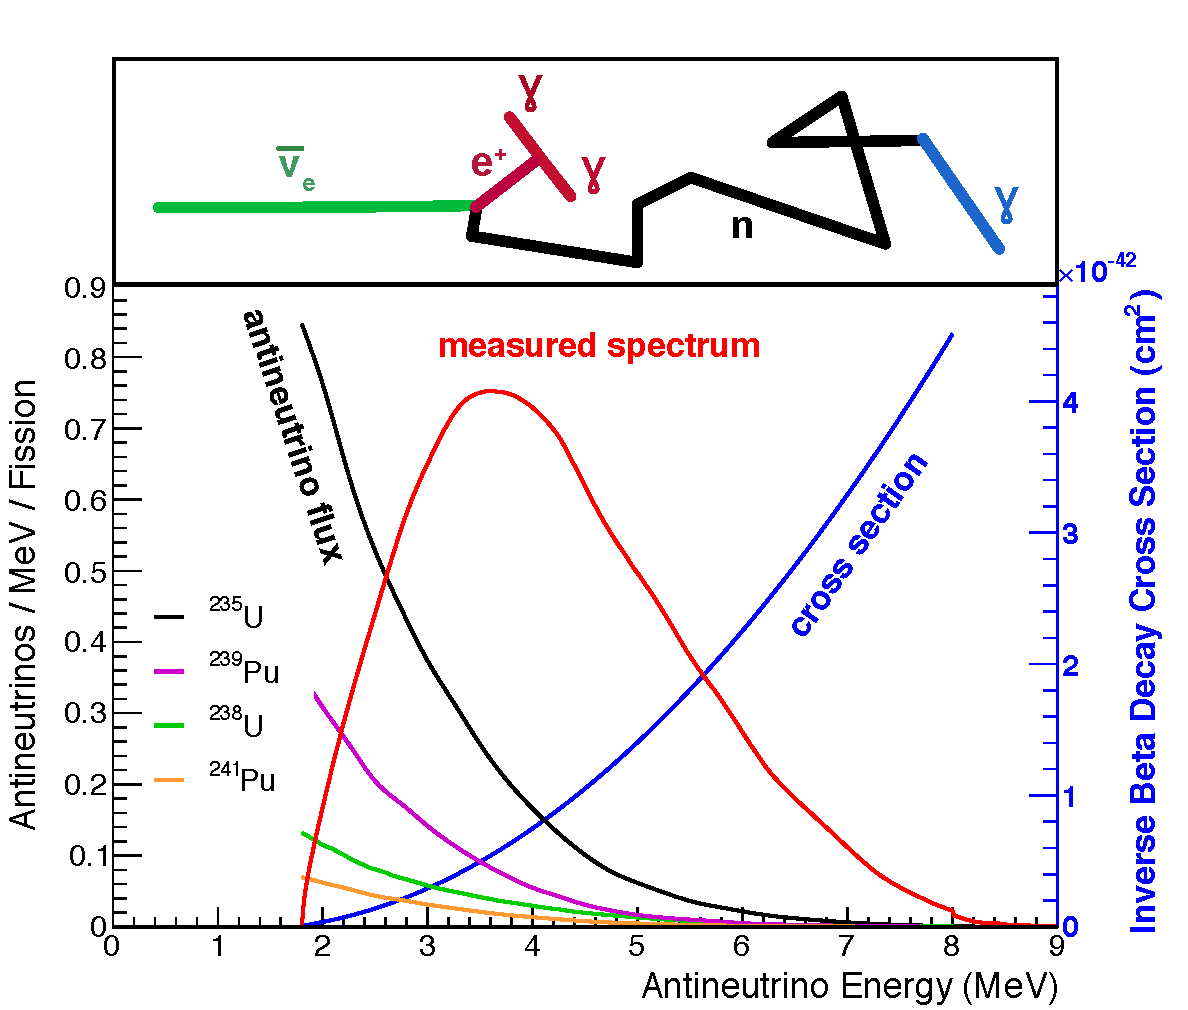
\includegraphics[width=0.9\linewidth]{Img/Figure-2.pdf}
\bicaption[通过 IBD 测得的反应堆中微子能谱与四种核素产生的中微子流强构成]{图中红线为通过逆贝塔衰变（IBD）测量得到的预期反应堆中微子预期总能谱，蓝线为 IBD 反应截面随中微子能量的变化，彩色实线分别表示四种主要裂变核素（$^{235}\mathrm{U}$、$^{239}\mathrm{Pu}$、$^{238}\mathrm{U}$、$^{241}\mathrm{Pu}$）产生的中微子谱流强。顶部示意图给出 IBD 事件的关联事例（正电子与湮灭 $\gamma$）与延迟（中子俘获 $\gamma$）的偶然符合。图来自文献\citep{Vogel2015NeutrinoOscillation}}{Expected reactor antineutrino energy spectrum measured by the IBD reaction and component contributions. The red curve shows the expected total reactor antineutrino spectrum as measured via the inverse beta decay (IBD) channel (antineutrino energy per MeV per fission). The blue curve (right axis) gives the energy-dependent IBD cross section (cm$^2$). Colored solid lines denote the antineutrino fluxes produced by the four main fissile isotopes ($^{235}\mathrm{U}$, $^{239}\mathrm{Pu}$, $^{238}\mathrm{U}$, $^{241}\mathrm{Pu}$). The schematic above illustrates the typical prompt (positron and annihilation $\gamma$) and delayed (neutron capture $\gamma$) signals of an IBD event. The figure emphasizes the IBD sensitivity in the few-MeV region and the isotope-dependent spectral features relevant for reactor neutrino spectroscopy and oscillation analyses (figure from Ref\citep{Vogel2015NeutrinoOscillation}).}
\label{fig:reactor_ibd_spectrum}
\end{figure}

图~\ref{fig:reactor_ibd_spectrum} 展示了通过 IBD 反应测得的反应堆中微子能谱（红线）、IBD 截面（蓝线）与四种主要裂变核素的通量贡献（彩色曲线）；该图说明了不同核素对谱形的差异性以及IBD反应示意，因而精确的能量重建与谱学系统误差控制对振荡参数与质量顺序的测定至关重要。JUNO 探测器正是通过探测这些反应堆中微子与 LS 中自由质子的 IBD 相互作用，从而获取反应堆中微子通量和能谱信息，为中微子振荡参数的精确测定提供重要数据支撑。

在基于反应堆的中微子实验中，能量在数兆电子伏特（MeV）范围内的电子反中微子（$\bar{\nu}_e$）主要通过反贝塔衰变（Inverse Beta Decay，IBD）过程进行探测，即：

\begin{equation}
\bar{\nu}_e + p \rightarrow e^+ + n 
\end{equation}

该过程通常在液体闪烁体（Liquid Scintillator, LS）探测器中发生，得益于 IBD 相对较大的反应截面，这种探测方式具有优异的灵敏度和背景抑制能力。在这一反应中，反中微子与探测介质中的自由质子相互作用，产生一个正电子和一个中子。正电子在极短时间内将其动能通过电离损失沉积于探测器中，并与电子发生湮灭反应，释放出两个 511 keV 的伽马光子，形成“快信号”（prompt signal）；而中子经过热化过程后被周围的原子核俘获，随后释放出特征性的伽马光子，形成数百微秒尺度的“慢信号”（delayed signal）。快慢信号在时间和空间上的关联性可有效抑制自然放射本底和宇生粒子等非关联事例，因而 IBD 通道在实际实验中被广泛采用，尤其适用于反应堆中微子的精准测量与振荡研究。

在 IBD 相互作用中，正电子携带了绝大部分反中微子的能量。其动能通过在闪烁体中的沉积和湮灭产生闪烁光，进而被光电倍增管（PMTs）收集转换为光电子（photoelectrons, PE），再由电子学系统记录。由于正电子能量和入射中微子能量之间存在线性关系，且快信号具有良好的时间分辨，正电子能谱可作为反中微子能谱的有效代理量。然而，探测系统的非线性响应效应（nonlinearity, NL），包括闪烁体的非线性发光、切伦科夫光的贡献，光子传播过程的损耗以及电子学系统的增益不均等，会引起实际可见能量 $E^{\text{vis}}$ 与真实能量 $E_{\bar{\nu}_e}$ 之间的偏离。因此，实验中通常采用标定源（如 $\gamma$、$e^-$ 或 $\alpha$）进行能量响应刻度，并建立非线性修正模型。

以 JUNO 为例，其液体闪烁体的组分与大亚湾实验极为相似，实验利用精细的刻度系统和基于大亚湾经验的非线性模型，对能量响应进行了全面刻画。此外，JUNO 采用优化的能量重建算法和统计方法，实现了优异的能量分辨能力。这使得其能够高精度测量正电子的沉积能量谱，进而反推出反应堆中微子能谱，在中微子质量有序、混合角精确测量等物理目标上具有显著优势。

在此介绍本分析中在能量转换中使用的各个物理量以避免模糊。当中微子进入到液体闪烁体中，会产生正电子。中微子能量$E_{\bar{\nu}_e}$会转换为正电子能量$E_e$，这一过程与粒子散射的运动学相联系。正电子能量$E_e$是中微子与正电子散射角$cos\theta$与中微子能量$E_{\bar{\nu}_e}$的函数。当正电子发生堙灭时，其总能量换转换为沉积能量$E_{dep}$。考虑液闪非线性以及淬灭效应的影响，沉积能量$E_{dep}$转换为了可见能量$E_{vis}$。随后考虑探测器响应，可见能量$E_{vis}$转换为了重建能量$E_{dep}$。

\begin{equation}
\begin{aligned}
E_{\bar\nu_e}
&\xrightarrow{\text{kinematics}}
E_e(E_{\bar\nu_e},\cos\theta)
\xrightarrow{\text{annihilation}}
E_{\rm dep}(E_e)
\\
&\xrightarrow{\text{LS nonlinearity}}
E_{\rm vis}(E_{\rm dep})
\xrightarrow{\text{resolution}}
E_{\rm rec}(E_{\rm vis}) \, .
\end{aligned}
\end{equation}


重建能量能谱的计算见下式：

\begin{multline}
\phi(E_{\text{rec}}) = \int_{T_{\text{DAQ}}} \! \mathrm{d}t \int_{1.8\,\text{MeV}}^{15\,\text{MeV}} \! \mathrm{d}E_{\bar{\nu}_e} \, \phi(E_{\bar{\nu}_e}, t) \int_{-1}^{1} \! \mathrm{d}\cos\theta \, \frac{\mathrm{d}\sigma}{\mathrm{d}\cos\theta}(E_{\bar{\nu}_e}, \cos\theta) \cdot N_p \cdot \epsilon(E_{\text{dep}}) \cdot {} \\
\frac{1}{\sqrt{2\pi} \sigma_{E_{\text{vis}}}} \exp\left[-\frac{1}{2} \left(\frac{E_{\text{vis}} - E_{\text{dep}}}{\sigma_{E_{\text{vis}}}} \right)^2 \right]
\label{eq:phi-Erec-integral}
\end{multline}

其中：
$\phi(E_{\bar{\nu}_e}, t)$是时间间隔$t$时在探测器处的经振荡后的反应堆反中微子通量。$E_{\text{dep}} = E_{\text{dep}}(E_{\bar{\nu}_e}, \cos\theta)$ 表示由中微子能量和角度确定的沉积能量；$N_p$ 是靶质子数；$\epsilon(E_{\text{dep}})$ 是探测器对沉积能量的效率；$\sigma_{E_{\text{vis}}}$ 是探测器能量分辨。

为了将反应堆产生的反中微子能谱转化为实验中观测到的重建能谱，需要经过两个主要过程的卷积。首先，反中微子在探测器中与靶质子发生反应，按照微分散射截面 $\frac{d\sigma}{d\cos\theta}$ 分布产生一系列沉积能量事件，从而得到沉积能谱。该过程还包含了靶粒子数 $N_p$ 以及探测器效率 $\epsilon(E_{\text{dep}})$ 的影响。随后，沉积能谱再通过与探测器的能量响应函数（通常近似为高斯分布）进行卷积，最终得到重建能量谱 $S(E_{\text{vis}})$。这一过程在数学上体现为三重积分，分别对应中微子能量、角度散射以及探测器响应的卷积关系。
\subsection{JUNO的核反应堆}

JUNO 实验所探测的反应堆反中微子主要来自华南地区多个商用核电站。目前，对 JUNO 贡献最显著的是台山核电站和阳江核电站，如图\ref{fig:JUNO_location}所示，共包含八个反应堆堆芯。这些堆芯到探测器的基线长度集中在约 50 km 附近，其平均距离约为 52.5 km，使其成为 JUNO 进行中微子振荡精密测量的主要信号来源。
除上述主反应堆群之外，距离JUNO稍远的大亚湾核电站以及防城港核电站作为次要反应堆源也被纳入反应堆反中微子通量的计算。其反中微子通量不可忽略，因此在本分析中予以考虑。
台山、阳江以及大亚湾各反应堆堆芯的热功率、到探测器的距离以及对应的反 IBD 事例率，已在表 2-2 中进行了系统汇总。对于距离约 265 km 的惠州核电站，由于其仍处于建设阶段，预计将在 JUNO 开始运行后的数年内才具备发电条件，且具体时间表尚存在不确定性，因此未将其纳入本工作的主要物理结果分析中。
其余距离超过 500 km 的核电站对 JUNO 的反应堆反中微子事例率贡献较小，合计约为每天一个 IBD 事例量级。在本分析框架下，这部分超过 500 km 的远距离反应堆产生的反中微子被视为一种本底分处理。关于反应堆反中微子通量的计算方法及其相关系统不确定性，将在第 2.3 节中作进一步讨论。
\begin{figure}[htbp]
  \centering
  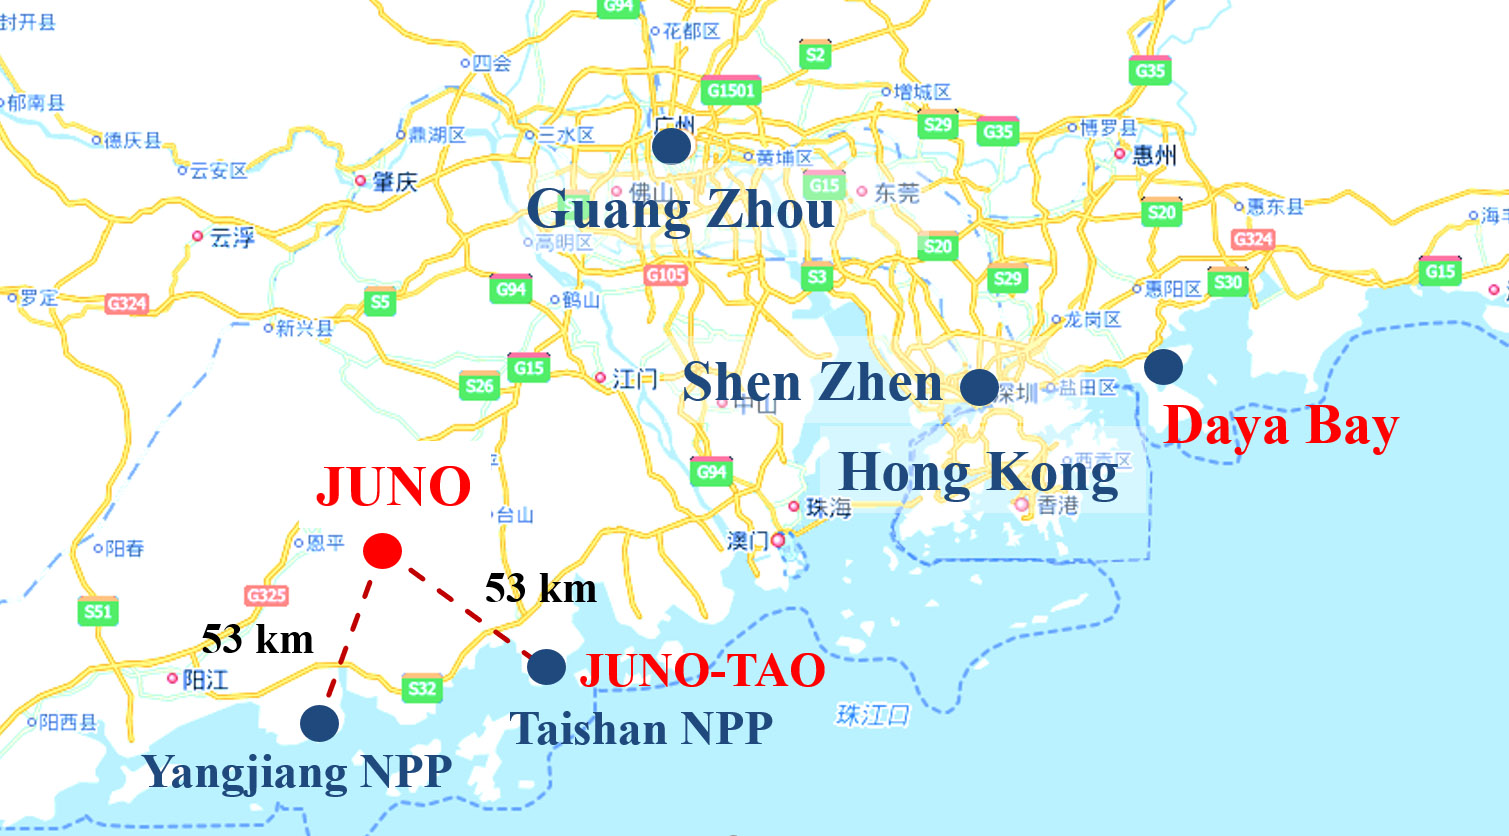
\includegraphics[width=0.9\linewidth]{Img/JUNO_location.jpg}
  \bicaption[JUNO探测器的位置]{JUNO探测器的位置}{JUNO detector location}
  \label{fig:JUNO_location}
\end{figure}

\subsection{反应堆反中微子通量的预测}
\label{sec:Arrived neutrino spectrum}

\subsubsection{反应堆反中微子能谱模型}
在商用轻水反应堆中，释出的电子反中微子主要来自若干主要裂变同位素的 β 衰变。为了构造到达探测器的中微子通量谱，常用两类方法：一种是基于转换法（conversion）得到的经验谱模型（代表性工作为 Huber–Müller 的基准谱）；另一种是基于裂变产物$\beta$支级信息的求和法（summation method），后者能够在理论上产生更丰富的谱形细节。本文以 Huber–Müller 模型作为基准反应堆谱用于生成参考到达谱，并以求和法产生的谱用于不确定度估计与谱形敏感性研究。本章分析中以 Huber–Müller 模型作为基准反应堆反中微子能谱模型，用以生成基准到达谱并作为后续不确定度评估和比较的参照。在后续不确定度量化与分 bin 策略研究中，将介绍 summation 法产生的带有精细结构的反应堆反中微子能谱模型。

对第 $r$ 个反应堆堆芯在时刻 $t$ 的中微子产额谱，可表示为
\begin{equation}
\phi_r(E_{\bar\nu},t)
= \frac{W_r(t)}{\sum_i f_{ir}(t)\,e_i}\sum_i f_{ir}(t)\,s_i(E_{\bar\nu}),
\label{eq:phi-r-reactor-spectrum}
\end{equation}
其中 $W_r(t)$ 为第 $r$ 个堆芯在时刻 $t$ 的热功率，$f_{ir}(t)$ 表示在时刻 $t$ 第 $r$ 个堆芯中第 $i$ 种裂变同位素的裂变份额（例如 $^{235}\mathrm{U}$、$^{238}\mathrm{U}$、$^{239}\mathrm{Pu}$、$^{241}\mathrm{Pu}$），$e_i$ 为第 $i$ 种裂变同位素每次裂变释放的平均能量，$s_i(E_{\bar\nu})$ 为第 $i$ 种裂变同位素每次裂变产生的反中微子能谱（基准由 Huber--Müller 给出或由求和法计算）。将各堆芯的到达谱按距离衰减与振荡概率叠加，可得探测器处的总到达通量：
\begin{equation}
\Phi(E_{\bar\nu},t)=\sum_r \frac{\phi_r(E_{\bar\nu},t)}{4\pi L_r^2}\,P_{\bar\nu_e\to\bar\nu_e}(E_{\bar\nu},L_r),
\label{eq:Phi-total-reactor-flux}
\end{equation}
其中 $L_r$ 为第 $r$ 个堆芯到探测器的基线距离， $P_{\bar\nu_e\to\bar\nu_e}$ 为电子反中微子的生存概率。

需要强调的两个额外修正项是：非平衡态（Non-Equilibrium, Non-Eq）与已乏燃料（Spent Nuclear Fuel, SNF）的贡献。一般地，堆芯中的短寿命裂变产物在开机初期或换料后并不处于完全稳态，这些非平衡贡献会在谱的若干能段产生小的附加分量；而乏燃料储存池中残余放射性也会向背景能谱提供长期、能谱上可辨的微小贡献。两者通常作为谱形的微小校正并入 $\phi_r$ 或作为独立项加入系统误差评估中（在高精度谱拟合和不确定度量化中不可忽略）。

\paragraph*{非平衡态（Non-Eq）}：部分裂变产物具有较长的半衰期（从数天到数年不等），因此在堆芯运行、功率变动或换料周期内，这些长寿命核素在瞬时并不处于生产与衰变的平衡态。它们的累积与衰变会在某些能段上产生额外的 $\beta$ 衰变贡献，从而在瞬时反中微子谱上引入能量依赖的微小修正。经验与文献研究表明，非平衡态对瞬时总通量的一般相对影响为亚百分比量级（常取约 $\sim 0.5$--$0.8\%$ 作为参考值）\citep{Huber2011_nonEq,PhysRevLett.134.201802}，但其谱形并非平坦，而是随能量呈小幅结构变化，因此在高精度谱拟合中不能完全忽略。

\paragraph*{乏核燃料（SNF）}：从堆芯卸下并置于冷却池的乏核燃料仍含大量长寿命裂变产物，若干同位素的 $\beta$ 衰变端点能量超过 IBD 反应阈值，因而在冷却过程中继续向周围环境（以及近场探测器方向）贡献微弱的反中微子通量。通过厂方的换料历史与 SNF 清单，识别出对 IBD 区间有贡献的长寿命同位素并对其剩余活度进行时间积分，是评估 SNF 贡献的标准做法。典型估计表明，SNF 对探测器的日平均通量贡献亦处于亚百分比量级（文献常给出约 $\sim 0.2$--$0.4\%$ 作为参考值）\citep{Ma2015_SNF,PhysRevLett.134.201802}，但在谱低能端或特定能段上其影响可相对放大，需在精密分析中考虑并作为系统不确定度来源之一。对于 SNF 贡献的详细计算方法及其在反应堆中微子通量中的作用，可参考 X. B. Ma 等人针对 Daya Bay 乏燃料贡献的研究\citep{Ma2015_SNF}

为将上述修正纳入基准谱，可写成
\begin{equation}
\phi_r^{\rm tot}(E_{\bar\nu},t)
= \phi_r^{\rm base}(E_{\bar\nu},t)
+ \phi_r^{\rm NonEq}(E_{\bar\nu},t)
+ \phi_r^{\rm SNF}(E_{\bar\nu},t),
\label{eq:phi-r-tot}
\end{equation}
其中 $\phi_r^{\rm base}$ 通常采用 Huber–Müller 或求和法得到的基准谱，$\phi_r^{\rm NonEq}$ 由对堆内长寿命产物的累积计算得到，$\phi_r^{\rm SNF}$ 则由冷却池中各 SNF 批次的残余放射性与几何-时间积分得到。上述两项修正既可作为谱的确定性修正项直接加入 $\phi_r^{\rm tot}$，也可在不确定度评估中作为可变项（例如通过生成一组扰动谱进行 toy-MC）来量化它们对振荡参数拟合结果的影响。

\subsubsection{反应堆相关输入不确定度处理}
在本研究中，我们对来自反应堆输入（Non-Eq、SNF、裂变能 $e_i$、裂变份额 $f_{ir}$ 等）的不确定度采取较为保守的处理方案。

1. \textbf{Non-Eq 与 SNF 的产额不确定度}

非平衡态（Non-Eq）与乏核燃料（SNF）对瞬时通量的相对影响本就处于亚百分比量级，但由于其估计具有较大模型与历史依赖性，本研究对这两类产额项采用保守置信区间：产额不确定度取 $30\%$（作为参考值并与文献/合作组当前实践一致）。在相关性处理上，Non-Eq 与 SNF 的产额不确定度在同一核电站（NPP）内部的各堆芯之间视为\textbf{完全相关}（即堆芯间该项同符号、同幅度浮动），而不同核电站之间视为\textbf{不相关}。对远场（contribution small）核电站，可将其作为平滑背景项处理，并在协方差矩阵中加入相应的方差分量。

2. \textbf{裂变能 $e_i$ 的不确定度}

裂变能 $e_i$ 定义为每次裂变最终以热功形式释放出来（已扣除中微子所带走的能量与被非裂变材料俘获的能量）。裂变能并非绝对常数，会随燃料组成、温度与中子谱出现微小变化。本文采用的近似平均值为（单位 MeV）：${}^{235}\mathrm{U}:202.36,\; {}^{238}\mathrm{U}:205.99,\; {}^{239}\mathrm{Pu}:211.12,\; {}^{241}\mathrm{Pu}:214.26$。为反映其不确定性，我们在构建总协方差矩阵时将裂变能的不确定度按“堆芯内部完全相关”的假设加入协方差（即在同一 NPP 内各堆芯归一化因子受同一裂变能波动影响）；不同 NPP 之间则视为不相关。裂变能对通量的作用主要通过归一化因子 $\sum_i f_{ir}(t)\,e_i$ 将热功 $W_r(t)$ 转换为裂变率，因此其不确定度可直接映射为谱的整体归一化不确定度。

3. \textbf{裂变份额 $f_{ir}(t)$ 的不确定度与相关性}

裂变份额随燃耗（burn-up）演化而显著变化，决定了各同位素对源谱的相对贡献。堆芯演化通常通过经过验证的燃料演化代码（如 APOLLO2/SCIENCE）结合运行与换料历史进行预测；Daya Bay 等实验证实这些预测与测量之间的偏差通常小于 $\sim 5\%$。基于此与合作组常用的经验，本文对单个同位素裂变份额取\textbf{相对不确定度 5\%}。在相关性处理上，裂变份额的不确定度在同一堆芯内部的不同同位素之间通过构造适当的相关矩阵反映（negative-correlation 等约束可强制总和守恒）；在堆芯间我们同样沿用保守策略：把裂变份额的不确定度在同一 NPP 内假定\textbf{完全相关}，不同 NPP 之间视为不相关。

除基准的 Huber–Müller 模型外，基于核数据库的求和法（summation method）能生成包含更多精细结构信息的能谱，这类谱对于评估反应堆模型依赖引入的系统误差尤为重要。因此，在后续的不确定度量化与分 bin 策略研究中，将同时使用 Huber–Müller 基准谱与由 summation 法产生的一组扰动谱作为输入，评估对振荡参数拟合的影响。


\begin{table}[!htbp]
  \bicaption[JUNO 主要反应堆堆芯信息（功率、基线与裂变份额）]{本表列出用于本文分析的主要反应堆堆芯信息，包括堆芯标识（CoreName）、所属核电站（NPP）、额定热功率（GW）、到 JUNO 的基线距离（km），以及四种主要裂变同位素 $^{235}\mathrm{U}$、$^{238}\mathrm{U}$、$^{239}\mathrm{Pu}$ 和 $^{241}\mathrm{Pu}$ 的裂变份额 $f_{235}$, $f_{238}$, $f_{239}$, $f_{241}$。裂变份额 $f_i$ 表示在给定时刻该堆芯裂变中由同位素 $i$ 贡献的相对比例，其数值随燃料燃耗演化而变化，本表给出为某一参考时刻的代表性取值。DYB（Daya Bay）与 FangChengGang（防城港）为远场反应堆群，其基线较远，对 JUNO 的贡献在本文中作为次要成分处理。}{This table lists the main reactor core information used in this analysis, including core identifier (CoreName), nuclear power plant (NPP), rated thermal power (GW), baseline distance to JUNO (km), and the fission fractions $f_{235}$, $f_{238}$, $f_{239}$, $f_{241}$ of the four main fission isotopes $^{235}\mathrm{U}$, $^{238}\mathrm{U}$, $^{239}\mathrm{Pu}$, and $^{241}\mathrm{Pu}$. The fission fraction $f_i$ denotes the relative contribution of isotope $i$ to fissions in that core at a given time; it evolves with fuel burn-up, and the values given here are representative at a reference time. DYB (Daya Bay) and FangChengGang are distant reactor groups; their baselines are large and their contributions to JUNO are treated as secondary in this analysis.}
  \label{tab:reactor_cores}
  \centering
  \footnotesize
  \setlength{\tabcolsep}{4pt}
  \renewcommand{\arraystretch}{1.2}
  \begin{tabular}{@{}l l r r r r r r@{}}
    \toprule
    CoreName & NPP & Power (GW) & Baseline (km) & $f_{235}$ & $f_{238}$ & $f_{239}$ & $f_{241}$ \\
    \midrule
    TS\_C1   & TS  & 4.09  & 52.77 & 0.67 & 0.08 & 0.22 & 0.03 \\
    TS\_C2   & TS  & 4.15  & 52.64 & 0.46 & 0.08 & 0.37 & 0.08 \\
    YJ\_C1   & YJ  & 1.91  & 52.74 & 0.55 & 0.07 & 0.30 & 0.07 \\
    YJ\_C2   & YJ  & 2.74  & 52.82 & 0.59 & 0.08 & 0.29 & 0.05 \\
    YJ\_C3   & YJ  & 2.86  & 52.41 & 0.50 & 0.08 & 0.35 & 0.07 \\
    YJ\_C4   & YJ  & 1.55  & 52.49 & 0.72 & 0.07 & 0.18 & 0.03 \\
    YJ\_C5   & YJ  & 2.47  & 52.11 & 0.58 & 0.08 & 0.30 & 0.05 \\
    YJ\_C6   & YJ  & 2.87  & 52.19 & 0.51 & 0.08 & 0.34 & 0.07 \\
    DYB\_6Cs & DYB & 15.90 & 215.00 & 0.55 & 0.08 & 0.31 & 0.06 \\
    FCG\_4Cs & FangChengGang & 9.28 & 411.00 & 0.58 & 0.07 & 0.30 & 0.05 \\
    \bottomrule
  \end{tabular}
\end{table}



为了获得到达探测器处的反中微子能谱，需将修正后的反应堆发射谱与反中微子在传播过程中发生振荡的存活概率 $P_{ee}(E_\nu, L_{dr})$ 相乘，其中 $L_{dr}$ 为反应堆 $r$ 到探测器 $d$ 的基线长度：
\begin{equation}
\phi_{r}(E_\nu, t) = \phi_r'(E_\nu,t) \cdot P_{ee}(E_\nu, L_{r})
\label{eq:phi-r-at-detector}
\end{equation}
此处中微子在物质中的传播将受到物质效应的影响，这由 Wolfenstein 最早提出~\cite{Wolfenstein1978}，并由 Mikheyev 和 Smirnov 进一步发展~\cite{Mikheyev1985}。因此$P_{ee}$ 包含了由中微子与地壳电子相互作用所引起的物质效应~\cite{Akhmedov2004}。


当反中微子在基线 $L_{dr}$ 上传播至探测器 $d$ 时，其味态成分根据上式中三种轻子味的振荡公式发生演化 带有物质效应的反中微子存活概率见图~\ref{fig:osc_prob}。

\begin{figure}[htbp]
\centering
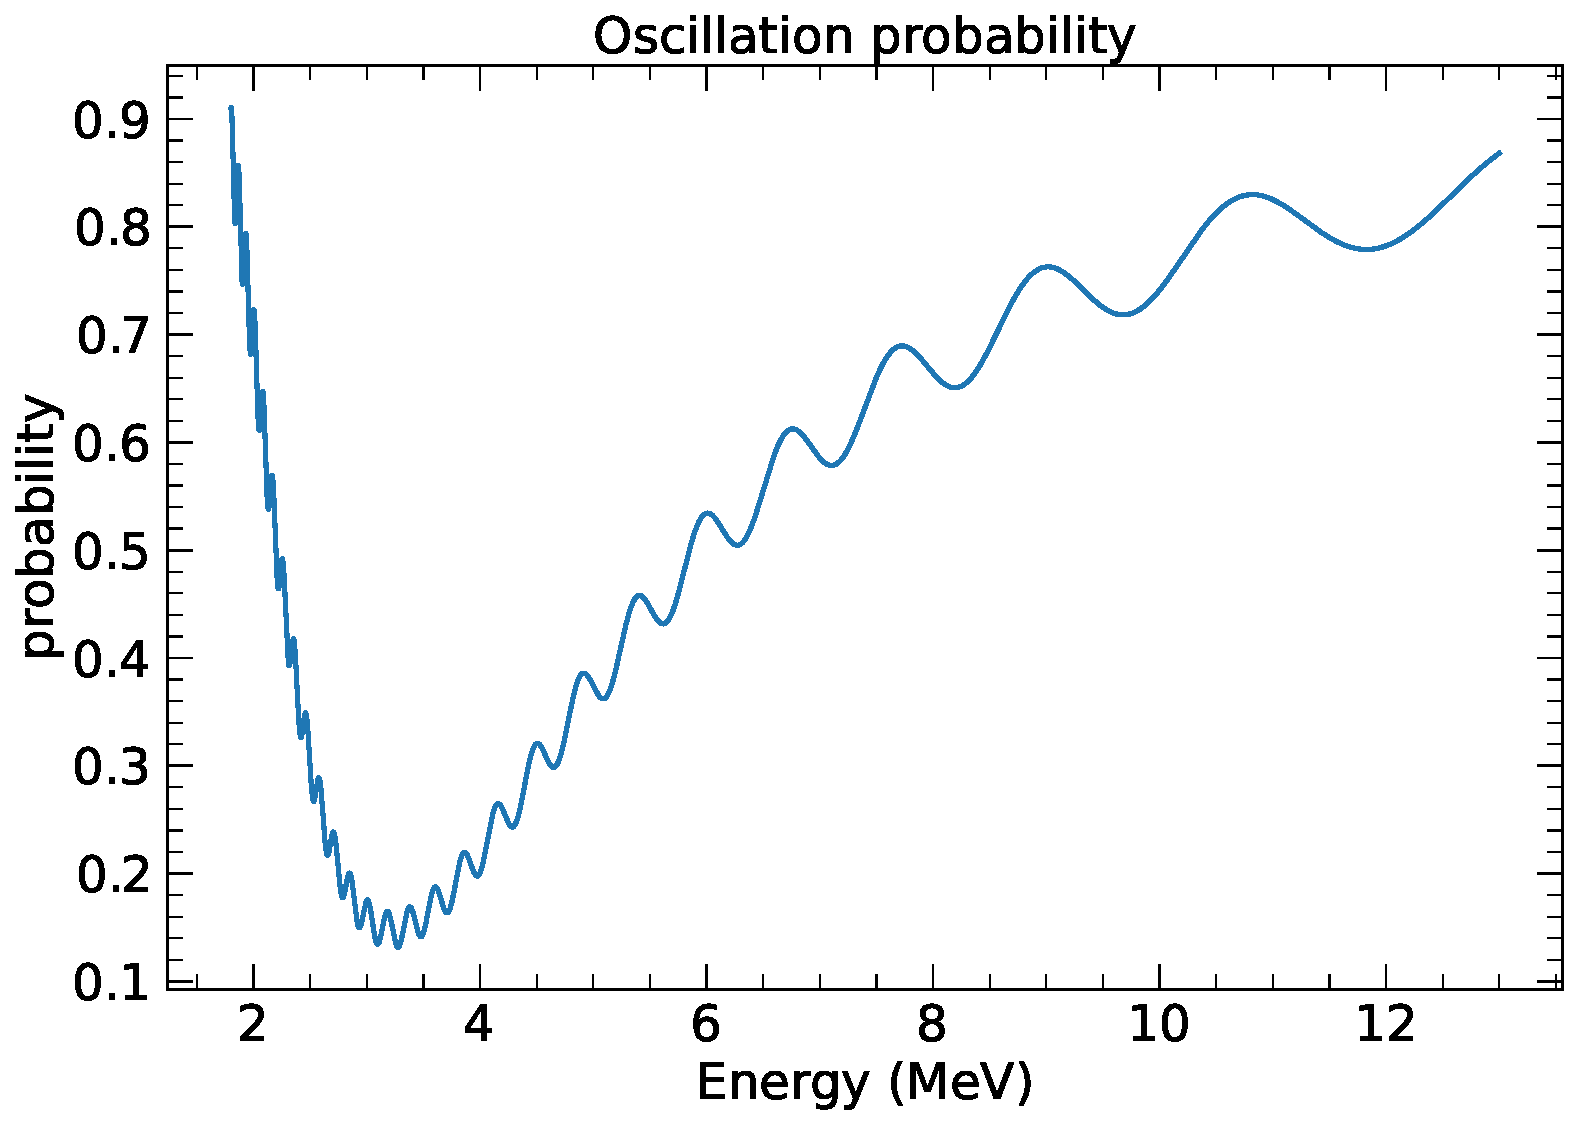
\includegraphics[width=0.6\textwidth]{Img/spectrum_cal/Oscillation_probability.pdf}
\bicaption{反中微子存活概率}{Electron antineutrino survival probability}
\label{fig:osc_prob}
\end{figure}

综上所述，通过引入乏燃料效应、非平衡修正及大亚湾经验修正因子，得到了更加精确的反应堆发射反中微子能谱 $\phi_r'(E_\nu,t)$。如图~\ref{fig:reactor_nu_arrival}，显示了核反应堆在裂变产物加权下的出射反中微子能谱（未考虑振荡），它作为后续到达谱与振荡折算的基准输入；进而结合恒定密度近似下的三味中微子振荡概率 $P_{ee}(E_\nu, L_r)$，可以计算得到到达探测器处的反中微子能谱 $\phi_{r}(E_\nu,t)$。  
如图~\ref{fig:reactor_nu_spectrum} 所示，将图~\ref{fig:reactor_nu_arrival}的出射谱与图~\ref{fig:osc_prob}中振荡概率以及几何衰减 $1/4\pi L^2$ 相乘后得到的实际到达探测器的能谱；加入振荡效应后，能谱中出现了随能量变化的振荡结构，反映了中微子质量本征态与味态之间的混合及传播演化行为。

\begin{figure}[ht]
  \centering
  \begin{subfigure}[t]{0.47\textwidth}
    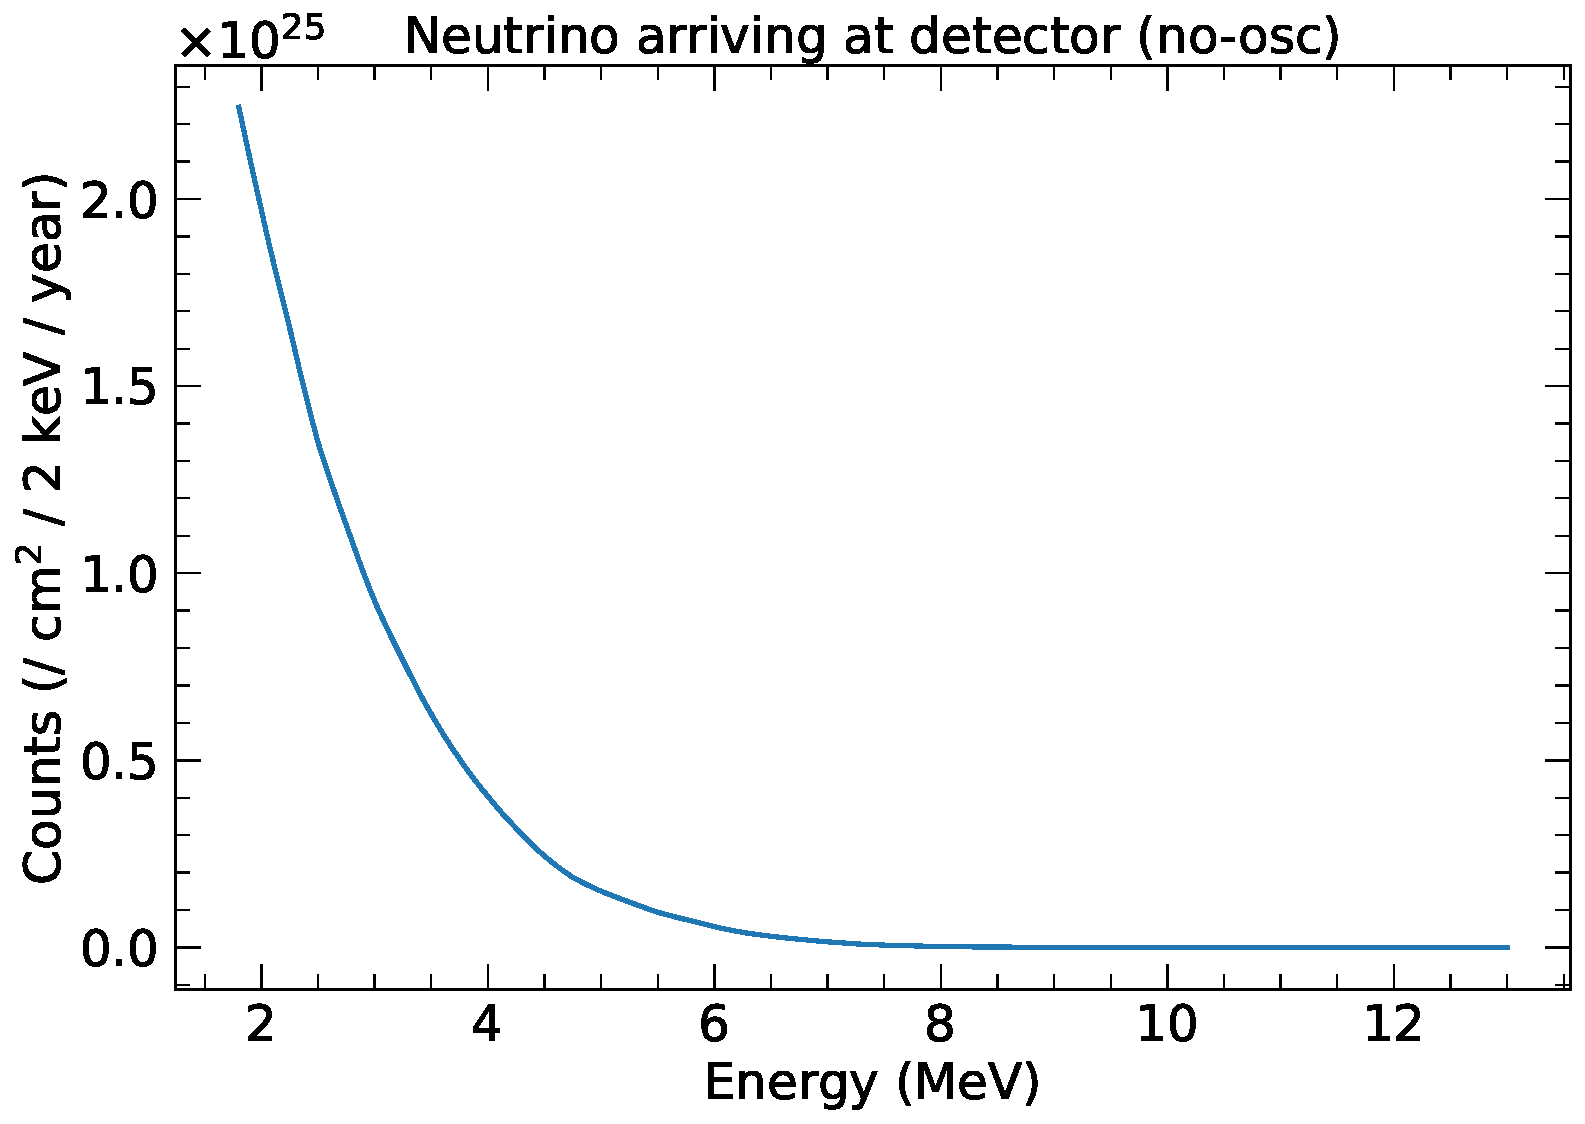
\includegraphics[width=\textwidth]{Img/spectrum_cal/Neutrino_arriving_at_detector.pdf}
    \caption{反应堆发射谱（未加振荡）}
    \label{fig:reactor_nu_arrival}
  \end{subfigure}%
  ~% add desired spacing
  \begin{subfigure}[t]{0.47\textwidth}
    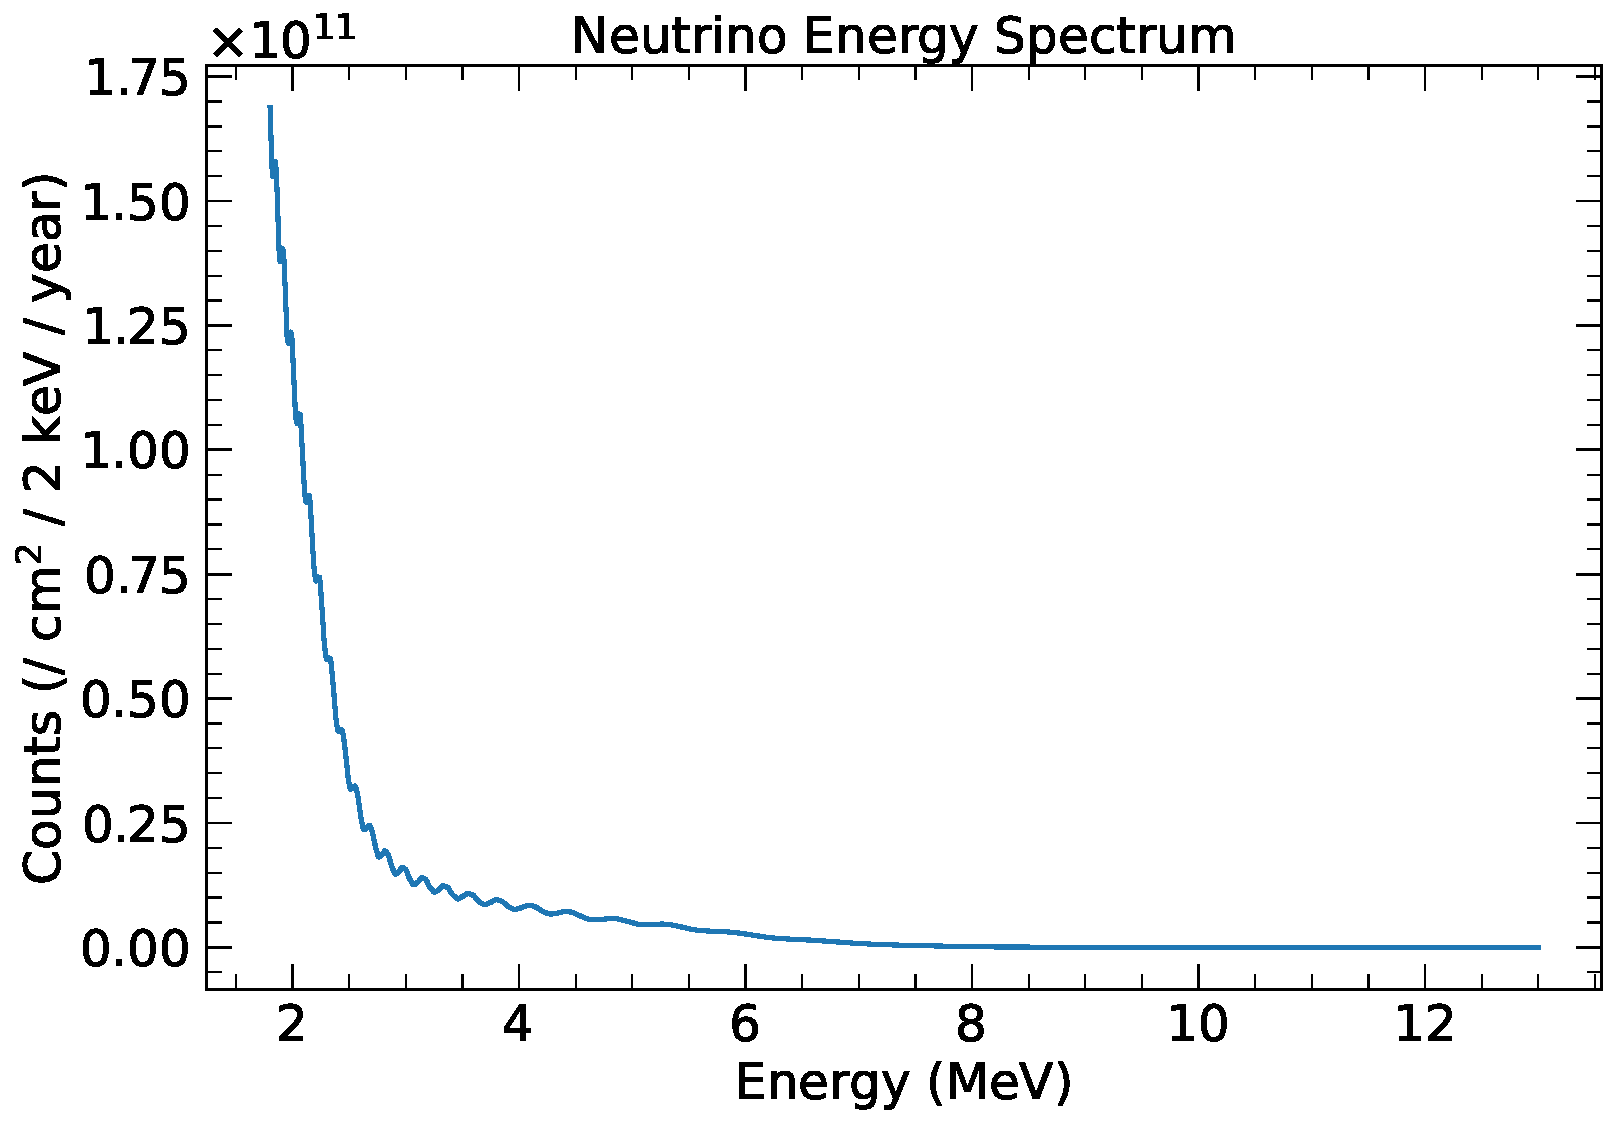
\includegraphics[width=\textwidth]{Img/spectrum_cal/Neutrino_energy_spectrum.pdf}
    \caption{中微子能谱}
    \label{fig:reactor_nu_spectrum}
  \end{subfigure}
  \bicaption{(a) 反应堆发射谱（未加振荡）：按裂变同位素加权并经归一化的电子反中微子能量分布；(b) 加入振荡与几何衰减后的探测器处预期能谱：将发射谱与存活概率以及 $1/4\pi L^2$ 因子相乘并按能量分bin得到的结果（单位为每 cm$^2$ 每年每能量bin计数）。}{(a) Reactor neutrino emission spectrum (no oscillation): the energy-dependent antineutrino yield per fission summed over fissile isotopes and normalized to reactor thermal power. (b) Predicted neutrino spectrum at the detector after oscillation and geometric attenuation: product of the emitted spectrum, oscillation probability and $1/4\pi L^2$ factors, shown here in units of counts per cm$^2$ per year per energy bin.}
\end{figure}



\subsection{沉积能量能谱}  
\label{sec:Deposited energy spectrum}

反应堆释放的反电子中微子能谱 $\phi(E_\nu)$ 通过逆贝塔衰变（IBD）反应与目标质子发生作用，产生正电子并沉积能量。探测到的沉积能量谱 $\phi(E_{\rm dep})$ 可表示为中微子能谱与 IBD 反应截面的卷积：  

\begin{equation}
\label{eq:continuous_rate}
\phi(E_{\rm dep}) \;=\; N_p \,  \int_{1.8}^{13} dE_{\overline{\nu}_e}\; \phi(E_{\overline{\nu}_e}) \; \frac{{\rm d}\sigma}{{\rm d}E_{\rm dep}}(E_{\overline{\nu}_e}, E_{\rm dep})  \; 
\end{equation}

其中 $N_p$ 为探测器中参与反应的自由质子数目，$\phi(E_{\overline{\nu}_e})$ 表示入射反应堆反电子中微子能谱。积分下限 $1.8\,\mathrm{MeV}$ 对应逆贝塔衰变反应的动力学阈值，而上限取 $13\,\mathrm{MeV}$ 以覆盖反应堆反中微子的有效能量范围。  
$\mathrm{d}\sigma/\mathrm{d}E_{\rm dep}(E_{\overline{\nu}_e},E_{\rm dep})$ 为关于沉积能量的 IBD 微分截面，它同时包含了反应截面的能量依赖性以及由散射角和反冲效应引入的动力学映射关系，刻画了给定入射中微子能量 $E_{\overline{\nu}_e}$ 时产生沉积能量 $E_{\rm dep}$ 的微分散射截面。

IBD 反应为 $\bar\nu_e + p \to e^+ + n$，仅当入射反中微子能量超过阈值 $E_{\nu}^{\rm th}\simeq 1.806\ \mathrm{MeV}$ 时才能发生。能量与动量守恒将入射中微子能量 $E_\nu$ 与产生的正电子总能量 $E_{e^+}$ 以及正电子的出射角 $\theta$（定义为中微子方向与正电子方向的夹角）联系起来。在零阶近似下（忽略质子反冲）正电子近似带走 $E_\nu$ 扣除中子–质子质量差 $\Delta=m_n-m_p$ 的能量，湮灭光子与正电子全能共同构成在闪烁体中沉积的能量 $E_{\rm dep}$，因此常用近似 $E_{\rm dep}\simeq E_\nu-0.78\ \mathrm{MeV}$ 作为直观估计。

为了获得更精确的能量映射和角分布权重，本工作采用 Vogel 与 Beacom 给出的 IBD 动力学与微分截面表达式（包括质子反冲等一阶修正及相应的角依赖项）来计算每一对 $(E_\nu,\cos\theta)$ 对应的正电子能量与微分截面 $\mathrm{d}\sigma/\mathrm{d}\cos\theta$（参见文献 \cite{Vogel1999Angular}）。基于该计算，对每个入射能量与发射角的样本点评估其产生的沉积能量并按微分截面加权，从而构造出用于离散化计算的响应矩阵 $M_{ij}$。该矩阵既包含了 IBD 截面的能量依赖性，也反映了由发射角和反冲效应引入的动力学展宽，是将入射中微子谱映射为沉积能量谱的关键数值单元。
\begin{equation}
E_{\rm dep}(E_\nu,\cos\theta)=E_{e^+}(E_\nu,\cos\theta)+m_e
\label{eq:Edep-positron}
\end{equation}
给定 $E_\nu$ 时，不同的 $\cos\theta$ 会产生略有不同的 $E_{\rm dep}$。低能下，IBD 的差分截面可以近似写为 $\frac{d\sigma}{d\cos\theta}\propto 1+v_e\,a(E_\nu)\cos\theta$，其中 $v_e$ 是正电子速率，$a(E_\nu)$ 与 $E_\nu$ 相关~\cite{Vogel1999Angular}。该式意味着在较低能量区，正电子角度分布近似均匀（$d\sigma/d\cos\theta\approx,$常数），只有微弱的方向依赖。基于上述动量学关系，可以将每个入射中微子能量 $E_\nu$ 和对应 $\cos\theta$ 映射到一个 $E_{\rm dep}$ 值，并用于构建响应矩阵。
\begin{equation}
\frac{\mathrm{d}\sigma}{\mathrm{d}E_{\rm dep}}(E_{\bar\nu},E_{\rm dep})
=\int_{-1}^{1}\!\mathrm{d}\cos\theta\;
\frac{\mathrm{d}\sigma}{\mathrm{d}\cos\theta}(E_{\bar\nu},\cos\theta)\;
\delta\!\bigl(E_{\rm dep}-T_e(E_{\bar\nu},\cos\theta)-m_e\bigr)
\label{eq:dsigma-dEdep}
\end{equation}
其中 $E_{\bar\nu}$ 表示入射反电子中微子能量，$T_e$ 为正电子的动力学能（kinetic energy），$m_e$ 为电子静质量。该式将中微子能量与正电子发射角 $\cos\theta$ 映射到可观测的沉积能量 $E_{\rm dep}$：对所有可能的发射角按角分布权重（由微分截面 $\mathrm{d}\sigma/\mathrm{d}\cos\theta$ 给出）进行积分，$\delta$ 函数保证仅在正电子产生的沉积能量恰好等于指定 $E_{\rm dep}$ 时才有贡献。换言之，式中积分把入射能量为 $E_{\bar\nu}$ 的中微子在不同发射角下产生的正电子能量分布累加起来，得到以沉积能量为自变量的微分截面。

物理上，$\mathrm{d}\sigma/\mathrm{d}\cos\theta$ 包含了 IBD 的角分布信息及与能量有关的动力学修正（例如质子反冲、一阶相对论展开项及必要的辐射学修正等；具体公式可参见 VogelBeacom (1999) 等文献）。$\delta$ 函数在理论上给出严格的能量映射，但在数值实现时通常以离散化方式处理：将 $\cos\theta$ 作等距或重要性采样，计算每一采样点对应的 $E_{\rm dep}$，并将该采样点按权重$\mathrm{d}\sigma/\mathrm{d}\cos\theta$ 累加到落入相应沉积能量区间的响应矩阵单元中。若需保留解析上的雅可比因子，可通过对 $\delta\bigl(E_{\rm dep}-T_e(\cos\theta)-m_e\bigr)$ 关于 $\cos\theta$ 的变换引入相应的导数因子；但在常见的蒙特卡洛或格点积分实现中，直接采样并归档权重的方法更加简便且数值稳定。

式中以角分布加权并对 $\cos\theta$ 积分的形式，明确给出了从入射中微子能量到可观测沉积能量的动力学映射关系；在数值实现上，$\delta$ 函数通过对角度采样并按微分截面加权归档到沉积能量区间来近似，从而得到用于后续响应矩阵构造的离散化微分截面。
经离散化后，上述连续映射可写为矩阵形式：
\begin{equation}
S_i \;=\; \sum_j M_{ij}\,\Phi_j,
\label{eq:Si-Mij-Phi}
\end{equation}
其中 $\Phi_j=\Phi(E_{\nu_j})\Delta E_{\nu_j}$ 表示第 $j$ 个中微子能量格点（或能量 bin）上的入射通量积分值，$S_i=S(E_{{\rm dep},i})\Delta E_{{\rm dep},i}$ 表示第 $i$ 个沉积能量格点上的期望事例数。响应矩阵元 $M_{ij}$ 编码了第 $j$ 个中微子能量 bin 的中微子通过 IBD 反应在第 $i$ 个沉积能量 bin 中产生信号的权重（权重包含微分截面、动力学映射與格点宽度等因素）。

在实际构造 $M_{ij}$ 时，常按如下数值流程实现：对每个入射能量格点 $E_{\nu_j}$ 在发射角 $\cos\theta\in[-1,1]$ 上做采样（等距或重要性采样），对每一采样点计算对应的正电子能量并由此得到沉积能量 $E_{\rm dep}=T_e+m_e$。该采样点的贡献按微分截面值 $\mathrm{d}\sigma/\mathrm{d}\cos\theta(E_{\nu_j},\cos\theta_k)$ 加权，并根据 $E_{\rm dep}$ 落入的沉积能量格点 $i$ 将该权重累加到 $M_{ij}$ 上。数值上可表达为求和形式：
\begin{equation}
M_{ij}=\sum_k \frac{\mathrm{d}\sigma(E_{\nu_j},\cos\theta_k)}{\mathrm{d}\cos\theta}\,\Delta\cos\theta\;
\mathbf{1}\bigl(E_{\rm dep}(E_{\nu_j},\cos\theta_k)\in [E_{{\rm dep},i},E_{{\rm dep},i+1})\bigr),
\label{eq:Mij-sum}
\end{equation}
其中 $\Delta\cos\theta$ 是采样步长，$\mathbf{1}(\cdot)$ 为指示函数（若条件成立取 1，否则取 0）。在实现时还常对中微子能量 bin 进行内部细分（sub-sampling）以提高数值精度，且在最终使用前对 $M_{ij}$ 做适当的归一化以符合定义（例如包含 $\Delta E_{\nu}$ 或在乘以 $\Phi_j$ 时一并处理）。

采用上述构造方法得到的响应矩阵自然同时包含了 IBD 微分截面的能量与角度依赖、由发射角和反冲引入的动量学展宽，以及离散化带来的能量混合效应。因此矩阵映射 $S_i=\sum_j M_{ij}\Phi_j$ 在数值上忠实再现了从入射反中微子谱到可观测沉积能量谱的完整物理过程。由基准反应堆通量与构建好的 $M_{ij}$ 得到的典型沉积能量谱示例见图~\ref{fig:depo_e_spec}。

下面给出构建响应矩阵 $M_{ij}$ 的伪代码流程示例（无探测器分辨率等效应），步骤清晰地描述了从中微子能量和角度采样到沉积能量归档的过程：
\begin{algorithm}[htbp]
\caption{生成响应矩阵 $M[i][j]$ 的伪代码}
\begin{algorithmic}[1]
\Require 中微子能量 bins $j$（中心能量 $E_{\nu_j}$），细分 $E_\nu$ 数 $n_{\text{split}}$，余弦角 bin 宽度 $\Delta\cos\theta$
\Ensure 响应矩阵 $M[i][j]$

\ForAll{中微子能量 bin $j$}
  \State $E_{\nu}^{\text{low}} \gets E_{\nu_j}^{\text{left}}$，$E_{\nu}^{\text{up}} \gets E_{\nu_j}^{\text{right}}$，$\Delta E_\nu \gets E_{\nu}^{\text{up}} - E_{\nu}^{\text{low}}$
  \For{$k = 0$ to $n_{\text{split}} - 1$}
    \State $E_{\nu_k} \gets E_{\nu}^{\text{low}} + \left(k + \frac{1}{2}\right) \cdot \frac{\Delta E_\nu}{n_{\text{split}}}$
    \For{$\cos\theta = -1$ to $+1$ step $\Delta\cos\theta$}
      \State 计算正电子动能：$T_1 \gets E_e(E_{\nu_k}, \cos\theta) - m_e$
      \State 计算沉积能量：$E_{\text{dep}} \gets T_1 + 2m_e$，查找 $i$ 使得 $E_{\text{dep}} \in [E_{\text{dep},i}, E_{\text{dep},i+1})$
      \If{找到合法的 $i$}
        \State 计算微分截面：$\frac{d\sigma(E_{\nu_k}, \cos\theta)}{d\cos\theta}$
        \State $\text{weight} \gets \frac{1}{n_{\text{split}}} \cdot \frac{d\sigma}{d\cos\theta} \cdot \Delta\cos\theta$，$M[i][j] \gets M[i][j] + \text{weight}$
      \EndIf
    \EndFor
  \EndFor
\EndFor
\end{algorithmic}
\end{algorithm}




1. 能量分箱：预先定义离散的中微子能量网格和对应的沉积能量网格。
    
2. 角度采样：对每个中微子能量 $E_{\nu_j}$，在 $\cos\theta\in[-1,1]$ 上均匀采样若干点。
    
3. 动量学转换：对每个 $(E_{\nu_j},\cos\theta_k)$，利用 IBD 动量学关系计算正电子全能 $E_{e^+}$，然后得到沉积能量 $E_{\rm dep}=E_{e^+}+m_e$。
    
4. 归档计数：根据 $E_{\rm dep}$ 所在的能量 bin $i$ 将该条事件计入响应矩阵：$M_{ij}+= (d\sigma/d\cos\theta)\Delta\cos\theta$。其中差分截面 $d\sigma/d\cos\theta$ 在每个样本点提供权重，$\Delta\cos\theta$ 是取样间隔。
    
5. 循环累积：对所有中微子能量 bin 和角度样本重复以上过程，最终得到完整的微分散射截面矩阵 $M_{ij}$。
因此微分散射截面矩阵的构建逻辑是先采样中微子能量和出射角度，计算对应的沉积能量，并将相应的微分截面权重累加到正确的能量 bin 中。这样，矩阵 $M_{ij}$ 自动反映了从入射中微子谱到探测沉积谱的完整物理映射关系。
最终，沉积能量能谱可以通过下式得到：
\begin{equation}
\phi_{\rm dep} = \phi_{\nu} \cdot M_{ij}
\label{eq:phi-dep-Mij}
\end{equation}
沉积能量能谱见图~\ref{fig:depo_e_spec}。

\begin{figure}[htbp]
\centering
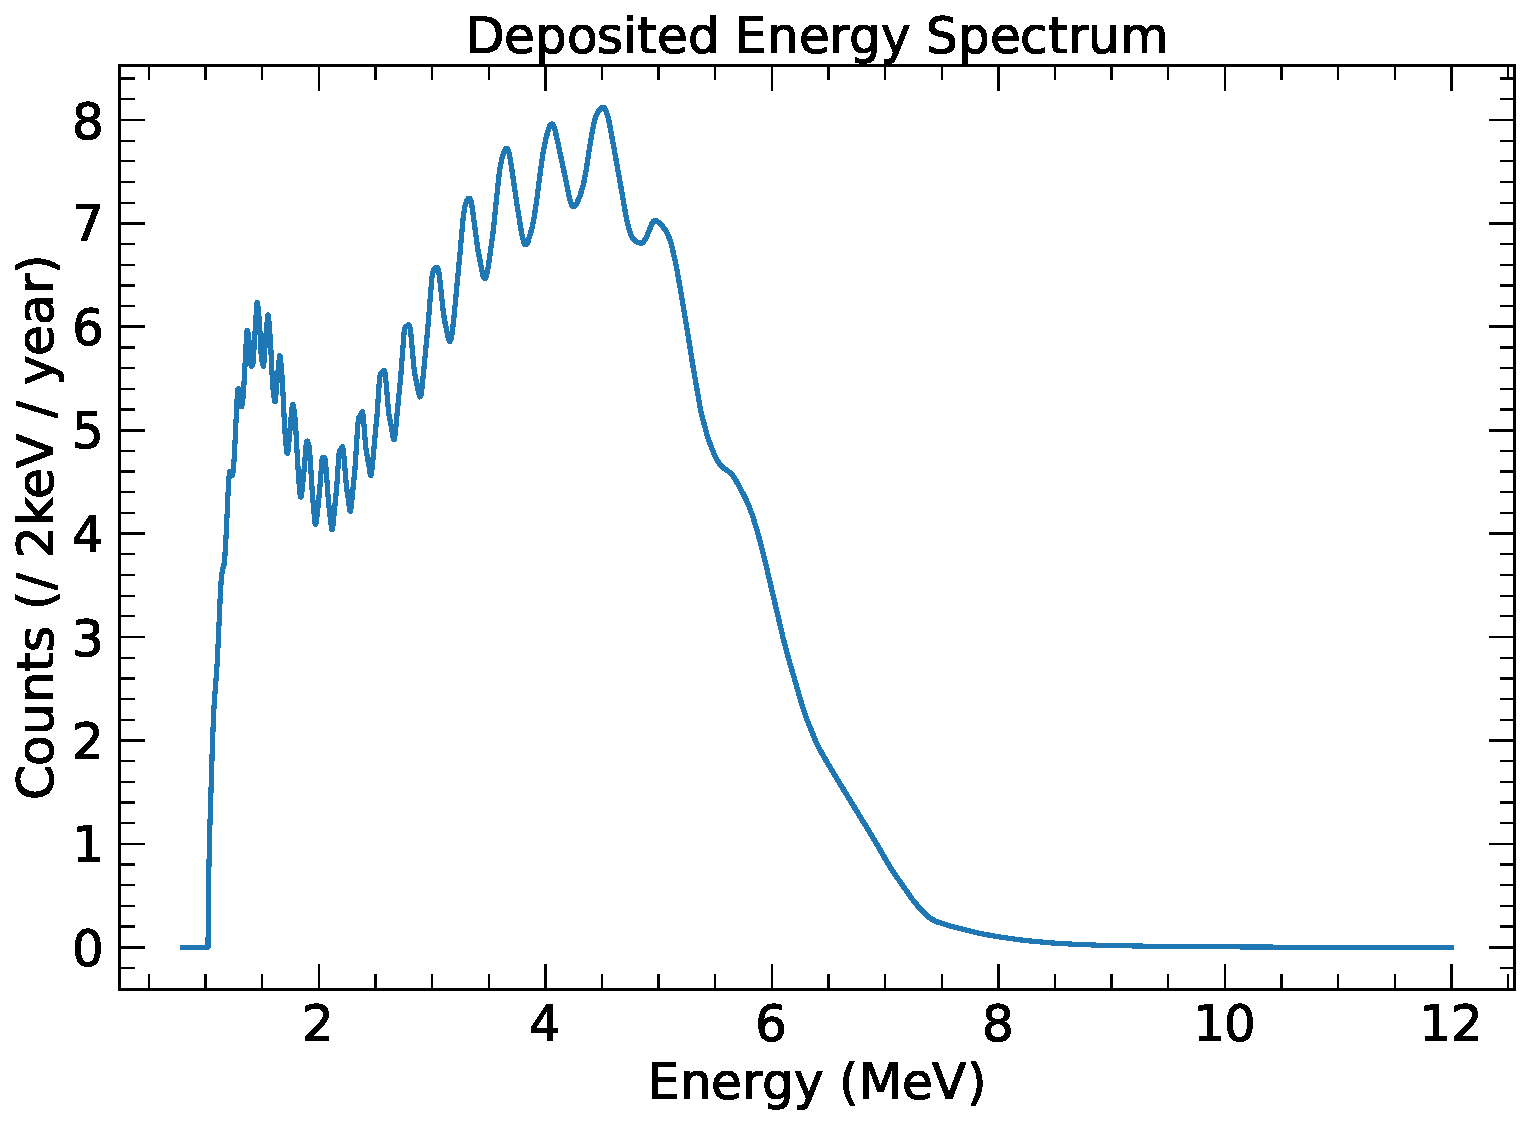
\includegraphics[width=0.6\textwidth]{Img/spectrum_cal/Deposited_energy_spectrum.pdf}
\bicaption{沉积能量能谱}{Deposited energy spectrum}
\label{fig:depo_e_spec}
\end{figure}

\subsection{重建能量能谱}
\label{sec:Reconstructed energy spectrum}
粒子在闪烁体中沉积的能量经过闪烁体本征非线性响应与探测器分辨效应后，最终以重建能量 $E_{\rm rec}$ 的形式被记录下来。重建过程通常分为两步：先将沉积能量映射为可见能量（非线性校正），然后将可见能量以测量误差（能量分辨）随机展宽得到重建能量分布。

首先，闪烁体的非线性响应由经验/校准模型 $f_{\rm LSNL}$ 描述，将沉积能量 $E_{\rm dep}$ 映射为可见能量 $E_{\rm vis}$：  
\begin{equation}  
E_{\rm vis} = E_{\rm dep}f_{\rm LSNL}(E_{\rm dep}) .  
\end{equation}  
函数 $f_{\rm LSNL}(E)$ 随能量变化，涵盖了淬灭（quenching）、Cherenkov 光贡献及其它探测器特异性的非理想效应。通常先通过校准数据确定 $f_{\rm LSNL}$ 的参数与不确定度，得到校正后的期望可见能量记作 $E_{\rm vis}^0$。
可见能量的计算通过下式
\begin{equation}
E_{\rm vis} = E_{\rm dep}\,f_{\rm LSNL}(E_{\rm dep})
\label{eq:Evis-LSNL}
\end{equation}
这里 $f_{\rm LSNL}$ 随沉积能量而变化，将粒子能量损失映射到闪烁光产额。得到 $E_{\rm vis}^0$ 后，还需考虑探测器的能量分辨效应。通常假设分辨函数为高斯型，即重建能量 $E_{\rm rec}$ 服从以均值 $E_{\rm vis}^0$ 为中心的高斯分布，其标准差按经验给出：
\begin{equation}
\sigma_{E_{\rm rec}} = E_{\rm vis} \sqrt{\frac{a^2}{E_{\rm vis}} + b^2 + \frac{c^2}{(E_{\rm vis})^2}}
\label{eq:sigma-Erec}
\end{equation}
其中参数 $a,b,c$ 分别对应光子统计、系统误差和噪声等贡献~\cite{An2021Unfolding}。该形式体现了分辨率随光子计数的泊松涨落、非均匀性和仪器噪声而变化的综合效应。相对分辨率形式~\cite{An2021Unfolding}如下
\begin{equation}
\sigma_{E_{\rm rec}}/E_{\rm vis} = \sqrt{a^2/E_{\rm vis} + b^2 + c^2/E_{\rm vis}^2}
\label{eq:sigma-Erec-rel}
\end{equation}
基于上述处理，可构建探测器响应矩阵 $R_{ij}$，用于将真实的沉积能量谱映射为重建能量谱。具体地，将能量空间离散为一系列能量小区间（bins）。对每个沉积能量小区间 $E_{\rm dep}^{(j)}$，重建能量 $E_{\rm rec}$ 的分布由上述高斯响应给出，因此在第 $i$ 个重构能量区间内出现的概率可由高斯分布的累积分布函数(CDF)计算：
\begin{equation}
\mathrm{CDF}(E_{\rm rec}^{(i)} \mid E_{\rm dep}^{(j)}) = \frac{1}{2}\Bigl[1 + \operatorname{erf}\Bigl(\frac{E_{\rm rec}^{(i)} - E_{\rm vis}}{\sqrt{2}\,\sigma}\Bigr)\Bigr]
\label{eq:CDF-Erec-Edep}
\end{equation}
这里 $\mu=E_{\rm vis}^0$ 为高斯分布均值，$\sigma$ 为上式给出的标准差；$\operatorname{erf}$ 为误差函数，满足 $\frac{1}{2}[1+\operatorname{erf}(x/(\sqrt2))]$ 为标准正态分布的 CDF。由此，第 $j$ 个沉积能量区间映射到第 $i$ 个重建能量区间的概率就是相邻两个阈值之间 CDF 的差值：
\begin{equation}
R_{ij} = \mathrm{CDF}(E_{\rm rec}^{(i+1)} \mid E_{\rm dep}^{(j)}) - \mathrm{CDF}(E_{\rm rec}^{(i)} \mid E_{\rm dep}^{(j)})
\label{eq:Rij-CDF}
\end{equation}
响应矩阵 $R_{ij}$ 既包含由 $f_{\rm LSNL}$ 引起的能量漂移（mean shift），也包含由能量分辨引起的展宽（smearing），能够准确描述沉积能量向重建能量的转换概率分布。
最终，任意给定的沉积能量谱 $\Phi_{\rm dep}(E_{\rm dep,j})$ 与响应矩阵相乘即可得到对应的重建能量能谱 $\Phi_{\rm rec}(E_{\rm rec,i})$：
\begin{equation}
\phi_{\rm rec}(E_{\rm rec,i}) = \sum_j R_{ij}\,\phi_{\rm dep}(E_{\rm dep,j})
\label{eq:phi-rec-Rij}
\end{equation}
通过将沉积能量谱与高斯响应函数卷积得到重建能量谱,见图~\ref{fig:recons_e_spec}：体现了探测器对原始中微子能谱的响应，即通过能量非线性校正和分辨率展宽对真实能量谱进行smearing”，从而得到可与实验数据直接比较的重建能谱。
通过将闪烁体中的能量淬火和光统计涨落等效应分离开来，先通过非线性修正得到理想可见能量，再通过高斯分布描述测量误差，最终通过响应矩阵系统地将理论沉积谱映射到实验观测谱，对中微子能谱的精确重建至关重要。
\begin{figure}[htbp]
\centering
\includegraphics[width=0.6\textwidth]{Img/spectrum_cal/Reconstructed_energy_spectrum.pdf}
\bicaption{重建能量能谱}{Reconstructed energy spectrum}
\label{fig:recons_e_spec}
\end{figure}
反应堆中微子能谱与重建能谱关系可写为：flux $\to$ cross-section $\to$ detector response $\to$ reconstruction。
\begin{equation}
N_{\text{reco}}(E_{\text{reco}})=
\int R(E_{\text{reco}},E_{\text{true}})\,
N_{\text{true}}(E_{\text{true}})\,\mathrm{d}E_{\text{true}}.
\label{eq:Nreco-response}
\end{equation}

\section{统计拟合方法}

我们基于分箱的重构能谱来进行振荡参数估计。设由振荡参数 $\theta$ 与一组系统不确定性（赘余）参数 $\alpha$ 所决定的理论预测分箱重建能谱谱为$\boldsymbol{T}(\theta,\alpha)$。其中 $\theta=(\sin^2\theta_{12},\Delta m^2_{21},\Delta m^2_{31},\sin^2\theta_{13})$。观测数据记为向量 $\boldsymbol{M}$（JUNO 的分箱观测能谱）。为同时考虑统计不确定性与多种系统误差，我们采用含拉项（pull terms）的最小二乘（$\chi^2$）方法构造目标函数并进行拟合，其一般化的表达式如式~\ref{chisq}所示。

\begin{equation}
  \chi^2 \equiv(\boldsymbol{M}-\boldsymbol{T}(\boldsymbol{\theta}, \boldsymbol{\alpha}))^T \cdot \boldsymbol{V}^{-1} \cdot(\boldsymbol{M}-\boldsymbol{T}(\boldsymbol{\theta}, \boldsymbol{\alpha}))+\sum_k\left(\frac{\alpha_k}{\sigma_k}\right)^2,
  \label{chisq}
  \end{equation}
将式~\ref{chisq}展开可得到完整形式~\ref{chisq_complete}，
JUNO 的 χ² 由数据项（残差平方和）与一系列表示系统不确定性的惩罚项（Gaussian pull）组成，形式为  
\begin{equation}
\begin{aligned}
\chi^2 \equiv\; & \sum_i^{N_{\rm bins}}\left(\frac{\left(M_i-T_i^{\mathrm{IBD}}(\boldsymbol{\alpha})-\sum_B^{\mathrm{Bkg}}\left[T_i^B \left(1+\alpha_B\right)\right]\right)^2}{\left(T_i^{\mathrm{IBD}}(\boldsymbol{\alpha})+\sum_B^{\mathrm{Bkg}} T_i^B\right)+\left(T_i^{\mathrm{IBD}}(\boldsymbol{\alpha}) \, \sigma_{\mathrm{shp}}^i\right)^2+\sum_B^{\mathrm{Bkg}}\left(T_i^B \, \sigma_{\mathrm{shp}}^B\right)^2}\right) \\
& + \left(\frac{\alpha_C}{\sigma_C}\right)^2
  + \sum_{r}^{\mathrm{Cores}}\left(\frac{\alpha_r}{\sigma_r}\right)^2
  + \left(\frac{\alpha_D}{\sigma_D}\right)^2
  + \sum_B^{\mathrm{Bkg}}\left(\frac{\alpha_B}{\sigma_B}\right)^2
  + \sum_{l=1}^4\left(\frac{\alpha_l}{\sigma_l}\right)^2 \\
& + \left(\frac{\alpha_{\mathrm{EScale}}}{\sigma_{\mathrm{EScale}}}\right)^2
  + \sum_{p}^{\mathrm{NPP}}\left(\frac{\alpha_{{\mathrm{Pow}},p}}{\sigma_{{\mathrm{Pow}},p}}\right)^2
  + \sum_{\eta=a, b, c}\left(\frac{\alpha_\eta}{\sigma_\eta}\right)^2
  + \left(\frac{\alpha_{\rho \mathrm{ME}}}{\sigma_{\rho \mathrm{ME}}}\right)^2 \\
& + \sum_{p}^{\mathrm{NPP}}\left(\frac{\alpha_{\mathrm{SNF},p}}{\sigma_{\mathrm{SNF},p}}\right)^2
  + \sum_{p}^{\mathrm{NPP}}\left(\frac{\alpha_{\mathrm{Non\mbox{-}Eq},p}}{\sigma_{\mathrm{Non\mbox{-}Eq},p}}\right)^2
  + \left(\frac{\alpha_{\mathrm{Th/U}}}{\sigma_{\mathrm{Th/U}}}\right)^2
  + \sum_{f}^{\mathrm{FF}}\left(\frac{\alpha_{{\mathrm{FF}},f}}{\sigma_{{\mathrm{FF}},f}}\right)^2
  + \sum_{f}^{\mathrm{FE}}\left(\frac{\alpha_{{\mathrm{FE}},f}}{\sigma_{{\mathrm{FE}},f}}\right)^2 \, ,
\end{aligned}
\label{chisq_complete}
\end{equation}
其中第一行为分箱数据项，分母包含统计方差与若干背景谱形不确定度项；第二行及后续项为对各类系统不确定性的 Gaussian 约束（拉项）。相关符号及赘余参数（pull parameters）的含义在下文“数据项符号说明”和“系统不确定性 pull term”两小节中统一列出。
\subsubsection*{数据项符号说明}

\begin{itemize}
  \item $i$：重建能量谱中的第 $i$ 个能量 bin。
  \item $M_i$：第 $i$ 个重构能量 bin 中的观测事件数（信号+背景）。
  \item $T_i^{\mathrm{IBD}}(\theta,\alpha)$：预测的 IBD 信号事件数，依赖振荡参数与各类系统参数。
  \item $T_i^{B}(\alpha_B)$：第 $B$ 类背景在第 $i$ 个 bin 中的预测值。
  \item $V_{ii}^{\mathrm{stat}}$：统计方差估计（见式~\eqref{eq:Chisq:CNP}）。
  \item $\sigma_{\mathrm{shp}}^B$：第 $B$ 类背景的谱形不确定度。
  \item $f$：裂变同位素索引，分别对应 $^{235}$U、$^{238}$U、$^{239}$Pu、$^{241}$Pu。
\end{itemize}

\subsubsection*{系统不确定性pull term}

各赘余参数（pull term）及其物理含义如下：

\begin{itemize}
  \item \textbf{反应堆与探测器整体归一化}
    \begin{itemize}
      \item $C$：反应堆相关的整体相关不确定性，用于描述所有反应堆共同的通量归一化偏差（如反应堆反中微子通量模型的不确定性）。
      \item $D$：探测效率不确定性，对应 IBD 事件整体探测效率（包括触发、选择效率等）的归一化误差。
      \item P：反应堆热功率不确定性，直接影响反中微子产生率的整体归一化。
      \item FE：裂变能量（fission energy）不确定性，影响由热功率换算得到的反中微子通量归一化。
      \item FF：四种裂变同位素的裂变份额（fission fractions）不确定性，采用协方差矩阵 $\rho_{\mathrm{FF}}$ 刻画其相关性。
    \end{itemize}
  \item \textbf{能量响应相关}
    \begin{itemize}
      \item EScale：绝对能量刻度不确定性，描述探测器能量标定整体偏移对重建能谱的影响。
      \item $l$：第 $l$ 条液体闪烁体非线性（LSNL）拉曲线参数，用于刻画能量非线性模型的不确定性对谱形的影响。
      \item $\eta=(a,b,c)$：能量分辨率参数，对应能量分辨率经验公式中光子统计项、非均匀性项和电子噪声项的不确定性。
      \item shp：能谱形状不确定性，用于描述反应堆反中微子谱或背景谱的 bin-to-bin 形变。
    \end{itemize}
  \item \textbf{本底相关}
    \begin{itemize}
      \item $B$：第 $B$ 类本底过程（如偶然符合本底、Bi-Po214，宇宙线次级粒子、大气中微子等），用于描述不同本底rate不确定度。
      \item Th/U：地球反中微子中 Th 与 U 同位素贡献比例的不确定性。
    \end{itemize}
  \item \textbf{反应堆运行相关}
    \begin{itemize}
      \item $p$：第 $p$ 座核电站，用于区分来自不同核电站的功率、乏燃料等不确定性。
      \item NonEq：非平衡修正项不确定性，反映短寿命裂变产物未达到平衡状态对反应堆反中微子谱的影响。
      \item SNF：乏核燃料（Spent Nuclear Fuel）不确定性，用于描述反应堆停堆后燃料产生的额外反中微子通量。
    \end{itemize}
  \item \textbf{物质效应}
    \begin{itemize}
      \item $\rho_{\mathrm{ME}}$：地球物质密度不确定性，用于刻画物质效应（matter effect）对振荡概率的修正。
    \end{itemize}
\end{itemize}
为兼顾 Neyman（$\sigma^2\approx M$）与 Pearson（$\sigma^2\approx T$）估计在低计数箱中的偏差问题，我们采用加权组合的统计方差（CNP 组合）：  
\begin{equation}  
V_{ii}^{\rm stat} \equiv 3\left(\frac{1}{M_i}+\frac{2}{T_i^{\rm IBD}+\sum_B T_i^{B}}\right)^{-1}.  
\label{eq:Chisq:CNP}  
\end{equation}  
该组合在数值上消除了 Neyman 与 Pearson 各自的第一阶偏倚，并能避免零计数箱导致的分母为零的问题，从而在近似泊松极限下改善参数估计的稳健性。
$\chi^2$的最小化采用 \texttt{iminuit} 软件包中的 MIGRAD 算法完成，该算法基于拟牛顿法和梯度信息，具有良好的收敛速度与数值稳定性。当期望最小化距离（EDM）低于设定阈值后，迭代终止并认为拟合收敛。通过对冗余参数进行剖面化（profiling），得到物理参数的最优估计及其不确定度。

\subsection{Wilks 定理与 Feldman–Cousins 方法}  
\label{sec:statistical method}

在高能物理与中微子数据分析中，参数置信区间的估计通常基于检验统计量 $\Delta\chi^2$ 的统计行为。Wilks 定理~\cite{Wilks:1938dza}在大样本极限下为构造置信区间提供了方便的近似：在满足一定正则条件的情形下（例如假设为嵌套、参数为内点且样本量充分大），一维情形下的检验统计量
\begin{equation}
\Delta\chi^2(\delta)=\chi^2(\delta)-\chi^2_{\min}
\label{eq:Delta-chi2}
\end{equation}
近似服从自由度为 1 的 $\chi^2$ 分布。因此，可以使用固定阈值来构造置信区间，例如 $\Delta\chi^2=1$ 对应约 68.27\% 的置信水平，从而实现高效的区间估计。

但是，Wilks 定理的适用依赖于若干正则条件，这些条件在反应堆与加速器中微子实验中并不总是成立。常见会破坏 Wilks 定理近似的情形包括：参数有边界（bounded parameters）、参数空间的非光滑或非正则性、似然面存在多重或不相连的极小值（由参数简并或谱形-振荡耦合引起）、以及样本量不足使渐近性质失效~\cite{Acero2022ProfiledFC,Ogawa1964}等。在这些非正则条件下，$\Delta\chi^2$ 的经验分布会偏离理想的 $\chi^2$ 分布，导致用固定 $\Delta\chi^2$ 阈值构造的置信区间不再具有名义上的覆盖率（coverage）保证。需要指出的是，低统计并非 Wilks 失效的唯一原因，但会放大非正则效应并使偏差更加显著~\cite{Cordeiro1995}。

为了解决上述问题并保证频率学意义上的正确覆盖率，可采用 Feldman–Cousins（FC）方法~\cite{Feldman_1998}。FC 方法的核心思想是通过大量伪实验（toy Monte Carlo）直接构造检验统计量在假设参数值下的经验分布，从而得到参数依赖的临界值 $\Delta\chi^2_{\rm crit}(\delta)$。具体地，对于每个假定参数点 $\delta_i$，生成大量基于该 $\delta_i$ 的伪数据样本并计算相应的检验统计量分布，然后在所需置信水平下取出临界值。实际数据在该点的 $\Delta\chi^2(\delta_i)$ 若不超过 $\Delta\chi^2_{\rm crit}(\delta_i)$，则该参数点被包含于构造的置信区间内。由于临界值是通过模拟获得的，FC 构造在参数受界、非正则或多峰情形下仍能保证所设置信度的频率学覆盖性。

然而，FC 方法的代价是显而易见的：要构建完整的一维（或更高维）参数相关的置信带，必须在多个参数点 $\{\delta_i\}$ 上分别生成大量伪实验并计算临界值；当问题包含大量赘余参数（nuisance parameters）或考察高维参数空间时，所需的计算量会呈指数级增长。对于需要在不同谱形假设、不同能谱分 bin、不同系统扰动下重复评估的反应堆拟合任务而言，这种计算负担尤其沉重，常常成为高精度统计推断中的主要瓶颈。

基于上述考量，反应堆中微子实验的数据分析不仅需要严谨的统计方法论（如在必要时使用 FC 以保证覆盖），还迫切要求构建高效、可扩展的谱拟合与伪实验生成框架。常见的加速手段包括但不限于：将谱预测與似然评估张量化以减少解释性语言的循环开销、对响应矩阵与中间结果进行缓存与稀疏化存储、对伪实验并行化调度（多核/集群/GPU）、采用重要性抽样或代理模型（surrogate model）在参数空间中近似临界值曲线、以及对冗余参数实施剖面化插值（profiling interpolation）以减少重复拟合次数。后续章节将详细介绍本工作中所实现的若干加速策略以及其在大规模 FC 构造与 toy-MC 研究中的性能表现。

\section{本章总结}
本章系统介绍了反应堆中微子振荡分析的理论与数值框架，为后续灵敏度研究与覆盖率检验奠定了基础。围绕“从反应堆到重建谱”的分析主线，本章在物理建模、数值实现与统计推断三个层面取得了以下结果。

在物理层面，本章介绍了从反应堆反中微子的产生、传播与 IBD反应，最后到探测器探测到的重建能量能谱，明确给出了从入射中微子能谱到重建能量能谱的映射关系，并系统刻画了微分截面、能量转换关系以及探测器非线性与能量分辨模型对谱形的影响。

在数值实现层面，本章的构建了张量化的谱生成框架。通过将反应堆能谱、IBD 微分截面矩阵、沉积能量转换以及探测器响应矩阵统一表示为高维张量运算，实现了谱生成流程的模块化与矩阵化表达。该实现方式在保持物理透明性的同时显著提升了计算效率与可扩展性，使多参数扫描、批量 toy-MC 生成以及协方差传播能够在统一框架下完成。

在统计推断层面，本章介绍了含pull term的 $\chi^2$ 构造形式，系统纳入反应堆、探测器与本底相关的不确定性来源，并采用 CNP 统计方差组合以降低低计数区间的偏倚问题。同时讨论了 Wilks 定理的适用条件与局限性，指出在非正则情形下需要借助 Feldman–Cousins 方法进行严格覆盖率评估，从而明确了后续加速拟合算法研究的必要性。

总体而言，本章完成了反应堆中微子振荡分析链条的形式化与数值化构建，实现了一个可计算、可扩展且物理自洽的拟合框架。这一框架不仅支持振荡参数的精确提取，也为后续章节中对计算效率优化与统计覆盖率检验的深入研究提供了坚实基础。

%=====================================================================
%=====================================================================
 %=====================================================================
\chapter{反应堆中微子能谱拟合程序的加速（Acceleration Strategies）}
%=====================================================================

在反应堆反中微子振荡的统计推断中，为确保置信区间的频率学覆盖率（Coverage），通常需采用 Feldman-Cousins（FC）方法对海量伪实验（Toy MC）进行拟合。针对存在参数简并或多重局部极小值（如 $\Delta m^2_{31}$）的物理问题，其计算需求随参数网格密度、伪实验样本量及多起点扫描策略的叠加呈指数级增长。总拟合规模往往达百万量级，导致传统的串行拟合方案在常规算力资源下难以为继。为了使高精度的覆盖率验证与广域参数扫描成为现实，必须在算法逻辑与工程实现层面对拟合程序进行系统性的加速优化。

本章设计并实现了一套基于 PyTorch 的前向折叠（Forward-folded）能谱拟合架构。针对 IBD 动力学映射（中微子 $\to$ 沉积能量）与探测器响应（沉积能量 $\to$ 重建能量）这两大性能瓶颈，采用了三项核心优化技术：(i) 结果缓存机制（Result Caching），大幅减少了昂贵的重复中间计算；(ii) 带状稀疏矩阵表示（Banded Sparse Matrix），利用响应矩阵的局域性特征降低内存带宽与计算开销；(iii) 分块张量化构造与分段卷积优化，利用张量并行处理能力最小化内存搬运。以 Intel Xeon Gold 6338 处理器作为基准测试平台，实验结果表明，上述优化使单次拟合速度较原始实现提升了约 7 倍，且数值相对误差控制在 $10^{-6}$ 量级以内（以双精度计算为基准）。该框架已成功应用于反应堆中微子振荡分析，为大规模 Feldman-Cousins 覆盖率研究提供了核心计算保障，并具有良好的通用性，可直接推广至其他基于前向折叠能谱分析的中微子实验。

本章的相关研究成果已发表于《欧洲物理期刊 C》（Eur. Phys. J. C, 2025 \cite{Xue2025HighPerformanceStatisticalMethods}），并被实验合作组采纳作为基础分析工具。本章组织结构如下：第~\ref{sec:problem_scale} 节量化分析大规模伪实验带来的计算挑战并明确加速的性能目标；第~\ref{sec:performance_analysis} 节通过性能剖析（Profiling）定位单次拟合中的主要计算瓶颈，并在此基础上提出分层优化策略；第~\ref{sec:techniques} 节详述结果缓存、带状稀疏矩阵表示与分块张量化构造等关键加速技术的实现细节，给出各项优化的基准测试结果，并量化重建能谱分箱尺度对拟合耗时的影响；第~\ref{sec:ch3_summary} 节对本章的加速方案与性能提升结果进行归纳。


\section{问题规模量化与性能目标}
\label{sec:problem_scale}

\begin{figure}[htbp]
    \centering
    
\includegraphics[width=0.8\textwidth]{"Img/accelerational importance.png"}
    \bicaption{加速重要性示意图}{Schematic illustration of the motivation for acceleration.}
    \label{fig:accelerational_importance}
\end{figure}

假设我们希望用 FC 方法得到某参数（例如 $\Delta m^2_{31}$）的 1$\sigma$（68\%）置信区间，如图~\ref{fig:accelerational_importance}所示，并采用下列设计：     

\begin{itemize}  
\item 在参数线上取 $N_{\rm pts}=50$ 个假定真值点 $\{\delta_i\}$，用于构造参数相关的置信带（confidence belt）；  
\item 每个真值点生成 $N_{\rm toys}=5000$ 个伪实验样本（toy）；  
\item 由于参数简并导致局域多极小，为避免拟合陷入假局部极小，对每个拟合初值使用 $N_{\rm init}=20$ 个不同的初始猜测并取全局最优（或等价地对多起点进行扫描）。  
\end{itemize}

则总拟合次数为

$$N_{\rm fits} \;=\; N_{\rm pts}\times N_{\rm toys}\times N_{\rm init}  
= 50 \times 5000 \times 20 = 5{,}000{,}000.$$

若采用传统拟合算法（逐个 toy、串行调用拟合器）且每次拟合平均耗时约 $t_{\rm fit}=150$ 秒，则总 CPU 时间为

$$T_{\rm tot} \;=\; \frac{N_{\rm fits}\times t_{\rm fit}}{3600\ \mathrm{s/h}}  
= \frac{5\times 10^6\times 150}{3600} \approx 2 \times 10^5\ \text{CPU·h},$$

该计算量约为 $2\times 10^5$ CPU·h。即便在大型计算集群（如 IHEP 集群）上同时调用 1000 个 CPU 核心，完成单次全量分析仍需约 200 小时，这在实际物理分析周期中难以接受。因此需要加速反应堆拟合程序，既要在算法层面（减少每次拟合的计算量）做优化，也要在系统架构层面（并行/分布式/缓存）做工程化支持。本章之后将介绍各项技术的实现细节与基准测试结果。

需要特别说明的是，上述估算基于直接使用 TAO-based bin2bin 谱形不确定性（bin-to-bin uncertain）作为信号谱的谱型误差描述，而没有把 TAO/Daya Bay 联合分析中额外引入的 per-reactor bin2bin 冗余参数以及联合似然的复杂性考虑进来。若将 TAO/DYB 的联合约束并入拟合流程，单次拟合的自由参数数目和计算成本都会进一步上升，从而使得总耗时更长，因此更需要加速反应堆拟合程序。


\section{性能瓶颈分析与分层建模}
\label{sec:performance_analysis}


为了定位反应堆中微子能谱拟合算法中的关键瓶颈，并将优化技术应用到最有效的环节，我们对单次拟合进行了性能剖析（profiling）。如图~\ref{fig:acc_time_distribution_in_one_fit}所示，谱计算（signal spectrum calculation）几乎完全主导了单次拟合的运行时间——约占总时间的98.6\%
（约 108.6 s），而最小化器及其它开销仅占约 1.4\%（约 1.5 s）。因此，若要显著缩短总拟合时间，相比于优化最小化器本身，优先加速信号谱计算更为关键。

\begin{figure}[htbp]
  \centering
  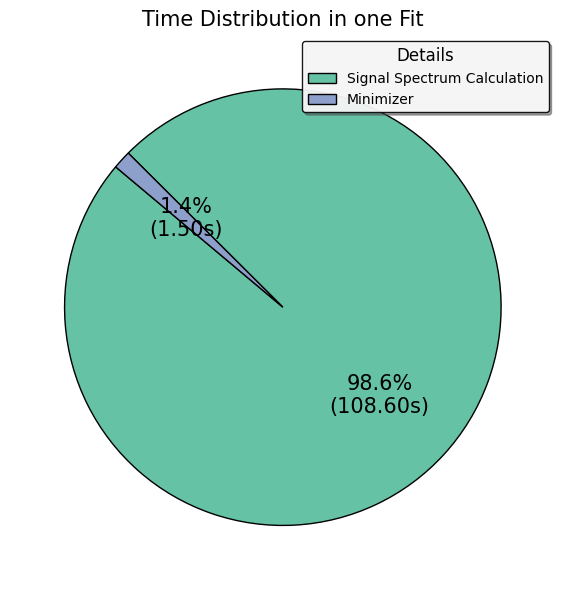
\includegraphics[width=0.55\textwidth]{Img/time_distribution_in_one_fit.png}
  \bicaption{单次拟合中各主要处理阶段的时间占比。谱计算（绿色）主导总耗时，而最小化器（紫色）仅占少量比例。}{Relative contributions of major processing stages in one fit. The signal spectrum calculation (green) dominates the runtime, whereas the minimizer (purple) accounts for only a minor share.}
  \label{fig:acc_time_distribution_in_one_fit}
\end{figure}

进一步对能谱计算任务进行细分（见图~\ref{fig:acc_time_distribution_in_signal_spectrum_calculation}），发现计算时间主要消耗于两项核心子任务：探测器响应矩阵的构建以及沉积能量谱的生成与映射。

\begin{figure}[htbp]
  \centering
  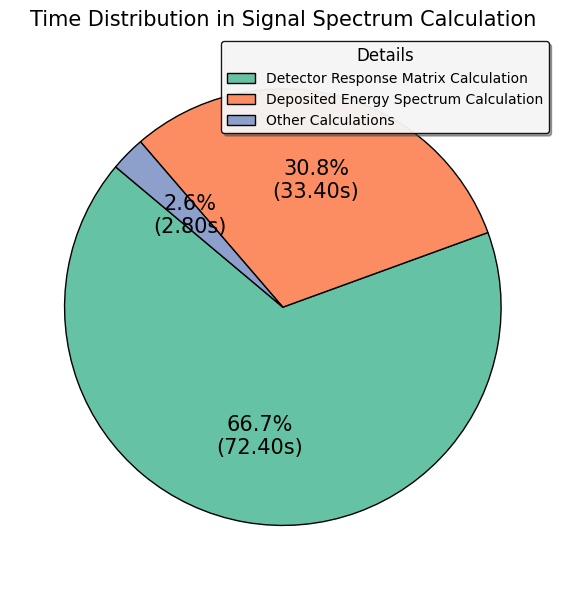
\includegraphics[width=0.55\textwidth]{Img/time_distribution_in_signal_spectrum_calculation.png}
  \bicaption{能谱计算内部的时间构成。探测器响应矩阵的计算（绿色）占多数，其次是沉积能量谱的生成（橙色），其余任务占比很小（蓝色）。}{Internal decomposition of the signal spectrum calculation. Most of the time is spent on the detector response matrix calculation (green), with additional contributions from the generation of the deposited energy spectrum (orange) and other minor tasks (blue).}
  \label{fig:acc_time_distribution_in_signal_spectrum_calculation}
\end{figure}

更细致的热点分析表明：
\begin{enumerate}
  \item \textbf{探测器响应矩阵计算}：在当前实现中，构造响应矩阵 \(R\) 需要对所有重建能量箱边界与可见能量采样点计算差值与归一化因子（大致对应一个 \(560\times5600\) 的减/除操作阵列），并对每个元素评估误差函数 \(\operatorname{erf}\) 以得到累积分布函数（CDF）。该过程伴随高强度的算术运算（Arithmetic Intensity）及大量特殊函数（误差函数 $\operatorname{erf}$）的调用。该环节耗时约 72.4 s，占谱计算总耗时的 66.7\%。         
  \item \textbf{沉积能谱计算}：这里的主要开销来自用微分散射截面（IBD mapping）矩阵将中微子能量映射到沉积能量的矩阵—向量乘法，在当前能量网格下，这等效于对约 $5600 \times 5600$ 维度的密集矩阵进行乘法运算，耗时约 33.4 s（占比 30.8\%）。
\end{enumerate}

基于上述剖析，本研究将优化重点放在两个热点之上，并制定相应的加速策略：
\begin{itemize}
  \item \textbf{响应矩阵加速}：对探测器响应矩阵计算采用分块构造，并可选地对 $\pm 6\sigma$ 区间进行截断，以减少误差函数 erf() 的无效计算。
  \item \textbf{IBD微分散射截面映射加速}：对 IBD 微分散射截面映射采用带状稀疏矩阵表示，利用其有限带宽特性采用稀疏乘法跳过大量零元素，从而降低内存与乘法开销。
\end{itemize}
此外，我们还引入了中间量缓存（caching）策略——对与物理参数无关且在多次拟合中重复使用的中间结果（例如响应矩阵的若干分块、固定的能量网格上的累积分布值等）进行缓存以避免重复评估。上述三类措施分别从减少特殊函数调用、降低矩阵运算复杂度与消除重复计算三方面切入，能够在不牺牲谱形精度的前提下，显著降低单次拟合的计算成本。


\section{加速策略实现与基准测试}
\label{sec:techniques}

\subsection{缓存技术}
\label{sec:caching}
在反应堆中微子能谱拟合中，往往伴随大量重复的矩阵运算与非线性变换——这些中间计算既占用 CPU 也带来频繁的 I/O。为降低重复计算开销、提高拟合与大规模 toy-MC 管线的整体吞吐量，我们在框架中引入了分层缓存机制（caching），以避免在参数估计和伪实验生成过程中对不必要的中间量反复求值。缓存策略主要在两个层面实施：

\textbf{静态量的预计算与常驻内存}

对于拟合过程中恒定不变的输入量，在拟合开始前一次性计算并加载到内存中。典型的静态量包括：

\begin{enumerate}
    \item 各裂变同位素的反中微子基准能谱 $\phi_i(E_{\bar{\nu}_e})$（如 ${}^{235}$U、${}^{238}$U、${}^{239}$Pu、${}^{241}$Pu）；
    \item IBD 的微分散射截面映射矩阵 $\sigma(E_{\bar{\nu}_e}\to E_{\rm dep})$；
    \item 探测器能量响应模型中的默认非线性响应曲线；
    \item 各类本底的谱形（如 Bi-Po214、宇宙线次级粒子、大气中微子、地球中微子、$^{13}$C($\alpha$,n)$^{16}$O 等）。
\end{enumerate}

将上述静态输入在拟合前预计算并常驻内存，一方面避免每次拟合或每次迭代时重复从磁盘加载，减少 I/O 开销；另一方面避免重复执行数值积分或插值，节省了大量 CPU 时间。

\paragraph{动态量的函数级复用（memoization）}
对于拟合过程中随参数变化、需要在每次迭代中更新的量（例如预测重建能量能谱、参数化能量非线性函数，或与响应矩阵及冗余参数组合相关的中间结果），其理论上需要逐次重新计算；但在实际拟合与大规模 toy-MC 中，常会出现\emph{相同输入反复出现}的情况。为避免重复求值，我们在函数层面引入缓存（memoization），实现上可直接使用 Python 标准库的 \texttt{functools.lru\_cache}（或等价的哈希缓存）。其核心思想是维护一个定长键值表：当相同参数的函数调用再次发生时，直接返回已缓存的结果而不进行数值计算。

\paragraph{数值实现注意事项}
对浮点参数而言，缓存命中要求参数的二进制表示（及其哈希）完全一致，因此默认情况下\textbf{不具备数值公差容忍}。工程实现中可通过以下方式提升命中率并控制误差：
\begin{itemize}
    \item 对浮点参数进行离散化/量化（quantization），例如按固定精度四舍五入后再参与哈希；
    \item 设计归一化的函数签名（统一单位与尺度、显式截断无关小数位），避免"数值等价输入"产生不同键值。
\end{itemize}

\paragraph{收益与可复用性}
函数级缓存对计算复杂且调用频繁的算子尤为有效，例如谱形卷积、矩阵乘法（或其分块子操作）以及误差函数 \(\operatorname{erf}\) 的批量评估。在广域参数扫描与 toy-MC 密集任务中，该策略可显著降低重复计算比例、提升整体吞吐量；基准测试表明，总拟合时间可降至约原来的三分之一（约 \(3\times\) 加速）。类似的缓存/预载策略在其他中微子分析框架中也已被验证有效，例如 GooStats 通过预载探测器响应网格实现了超过一个数量级的加速~\cite{Ding_2018}。本工作的缓存设计具有通用性，易于迁移到其它基于 forward-folded 能谱的实验分析，尤其适用于高维系统模型与大规模统计构造场景。

\subsection{微分散射截面矩阵的稀疏表示与响应矩阵分块优化}

\begin{figure}[htbp]  
    \centering  
    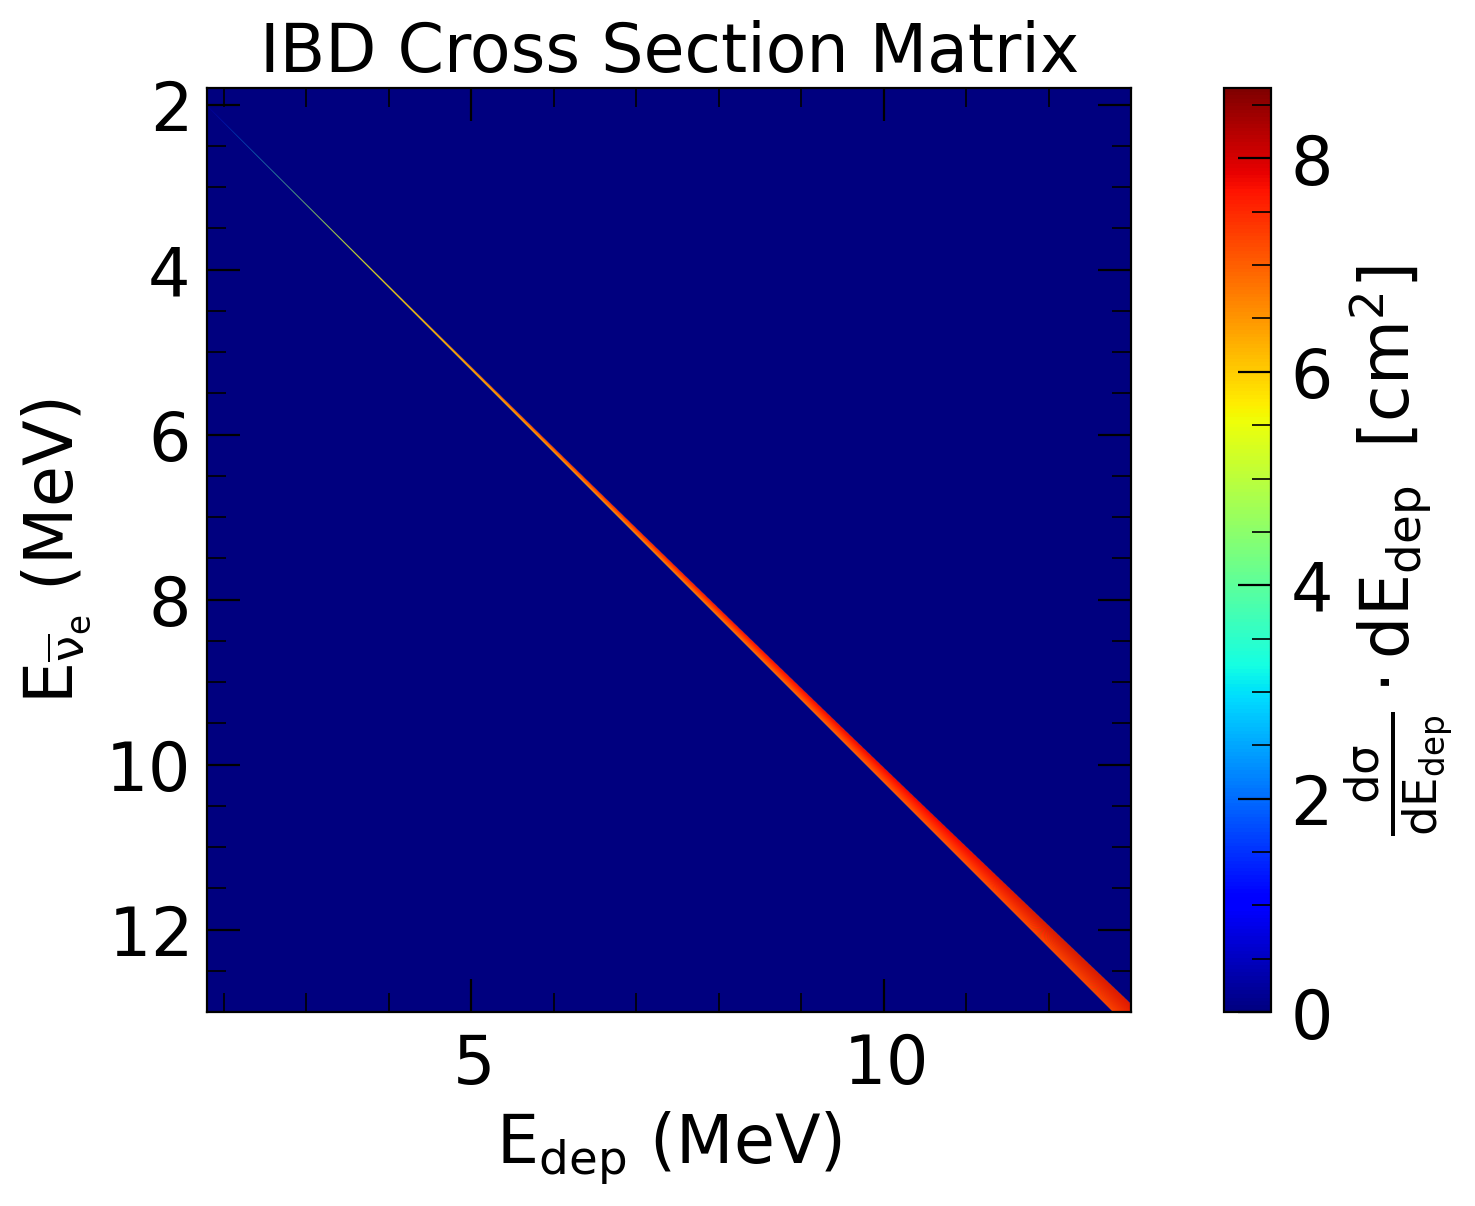
\includegraphics[width=0.55\textwidth]{Img/IBD_cross_matrix.png}  
    \bicaption{IBD 微分散射截面矩阵 $\dfrac{\mathrm{d}\sigma}{\mathrm{d}E_{\rm dep}}(E_{\rm dep},E_{\bar{\nu}_e})$ 的热力图（色标单位为 $10^{-44}$ cm$^2$ / 2 keV）。横轴为沉积能量 $E_{\rm dep}$（MeV），纵轴为入射反中微子能量 $E_{\bar{\nu}_e}$（MeV）；颜色越暖表示微分散射截面值越大。图中清晰可见主对角带，表明矩阵适合采用带状稀疏表示以加速谱的构造与拟合。}{Differential inverse beta-decay (IBD) cross-section matrix $\dfrac{\mathrm{d}\sigma}{\mathrm{d}E_{\rm dep}}(E_{\rm dep},E_{\bar{\nu}_e})$ is shown as a color map (color scale in units of $10^{-44}$ cm$^2$ per 2keV). The horizontal axis is the deposited energy $E_{\rm dep}$ (MeV) and the vertical axis is the incident antineutrino energy $E_{\bar{\nu}_e}$ (MeV); warmer colors denote larger differential cross-section values. This mapping is used to project theoretical neutrino-energy spectra into deposited-energy space for spectrum construction and fitting.}  
    \label{fig:sparse_cross_section}  
\end{figure}

在反应堆反电子中微子谱拟合中，从中微子能量 $E_{\bar{\nu}_e}$ 到沉积能量 $E_{\rm dep}$ 的映射由 IBD（逆贝塔衰变）微分散射截面控制，该映射可表示为二维响应矩阵 $M[i,j]$，其元素 $M_{ij}$ 表示入射能量为 $E_{\bar{\nu}_e,j}$ 的反中微子经 IBD 在沉积能量箱 $i$ 中产生信号的概率密度。受 IBD 动力学约束（尤其是正电子能量与发射角之间的耦合）影响，该矩阵呈现出明显的带状稀疏结构：非零元主要集中在主对角附近，满足近似关系

$$E_{\rm dep,i} \approx E_{\bar{\nu}_e,j} - \Delta,$$

其中 $\Delta\approx 0.8\ \mathrm{MeV}$ 包含了阈值与湮灭修正。该稀疏模式在图~\ref{fig:sparse_cross_section} 中有直观展示，主对角线附近有明显的带状结构。

鉴于大多数矩阵元素为零或接近零，我们采用 PyTorch 提供的稀疏存储格式（如 CSR/带状存储）来保存微分散射截面矩阵 $M$。稀疏格式只记录非零元素的位置与数值，从而显著降低内存占用并避免对零元的冗余计算。在谱生成与拟合过程中，响应矩阵 $M$ 与按振荡参数计算得到的中微子通量向量 $\boldsymbol{\phi}(E_{\bar{\nu}_e})$ 做乘法得到沉积能量谱 $S(E_{\rm dep})$。利用稀疏表示后，矩阵—向量乘法的计算复杂度可由 $O(N^2)$ 降为 $O(Nw)$，其中 $N$ 为能量格点数，$w$ 为带宽（非零元在对角带上的宽度），通常远小于 $N$，因此能获得显著的计算加速。

此外，稀疏表示在现代硬件（包括多核 CPU 与 GPU）上通常有更好的缓存局部性和更高的内存带宽效率，从而进一步提升并行计算中的吞吐量。我们的基准测试表明，在 Intel Xeon Gold 6338 平台上，不牺牲数值精度的前提下，采用稀疏表示与稀疏乘法可使微分散射截面映射步骤的计算时间缩短约 4 倍，成为整个加速管线中的关键组成部分。

类似的思想也被 ReMU 等框架采用：仅保留含非零元的行并结合高效的线性代数操作，以提升能谱构造效率~\cite{Koch2019}。总体而言，充分利用微分散射截面矩阵的稀疏性不仅能显著减少存储与计算开销，而且对中微子能谱拟合在高精度、低统计或大规模 toy-MC 分析下的可扩展性与性能影响深远。

\paragraph*{探测器响应矩阵的分块构造}\mbox{}\\
探测器响应矩阵用于将粒子在闪烁体中沉积的真实能量映射为对应的重建能量分布。矩阵的每个元素表示某一沉积能量落入某一重建能量箱的概率。在传统实现中，该响应矩阵通常为一个二维数组，尺寸约为 $560\times5600$：560 个重建能量箱对应横轴，5600 个沉积能量箱对应纵轴。构造该矩阵时，往往逐元素计算——先计算待测沉积能量与重建能量边界的差值，再除以标准差并对误差函数 $\operatorname{erf}$ 求值以得到累积分布函数（CDF），最后取相邻 CDF 的差值得到每个元素的概率。这种按元素计算的实现代价很高：一方面 $\operatorname{erf}$ 等特殊函数本身计算开销大；另一方面若一次性构造整个矩阵，则需在内存中保存大量中间结果，导致显著的内存占用与数据搬运开销。总体而言，逐元素一次性构造的方法在计算复杂度和内存消耗上都存在严重瓶颈。

为降低计算与内存负担，本工作采用了分块（block）处理策略：将 $560\times5600$ 的矩阵沿列方向切分为若干小的子块\cite{Lam1991}，并对每一子块逐个进行计算与累积。具体做法为：每次仅取出一个列区间内的沉积能量数据，在该区间上计算对应的重建能量概率分布；完成后将该子块的结果累加或拼接到最终的响应矩阵中，然后释放该子块的中间数据再继续处理下一个子块。这样一来，计算就被约束在较小的数据块上，有利于缓存（cache）重用并显著减少内存间的数据搬运；由于始终只保留当前子块的中间结果，无需为整个大矩阵分配峰值内存，从而大幅降低峰值内存使用与内存带宽压力。


分块计算方法在实践中带来了可观的性能提升。块宽的最优取值通过在测试平台（Intel Xeon Gold 6338）上对若干候选值（128、256、512、1024）进行基准测试确定：块宽 512 时耗时最短，这与其硬件对齐特性一致——512 为 2 的幂次（$2^9$），与 CPU 缓存行（cache line，通常 64 字节）对齐良好；512 个 float32 元素仅占 2 KB，可完整驻留于 L1 数据缓存（32 KB），从而最大化缓存命中率。块宽过小（如 128）时分块开销相对增大，过大（如 1024）时数据超出 L1 缓存导致命中率下降，故 512 为该平台上的经验最优值。在块宽设置为 512 时，探测器响应矩阵的构造时间从约 55 ms 降至约 27 ms，约为 $2\times$ 的加速比。该方法之所以有效，主要在于它充分利用了数据局部性（data locality），使得对 $\operatorname{erf}$ 等数值操作的调用更容易命中高速缓存，减少了重复 I/O 与索引开销，从而降低了整体运行时间与资源消耗。

\subsection{加速结果}
本节评估在中微子能谱拟合中应用各类优化技术所带来的性能提升。所有基准测试均在同一台服务器上进行，测试平台为 Intel Xeon Gold 6338（2.00 GHz）。我们考察了三类主要的加速策略：

\begin{enumerate}  
\item 引入缓存技术（caching）；  
\item 使用稀疏表示存储微分散射截面矩阵；  
\item 采用分块计算优化探测器响应矩阵的构造与乘法。  
\end{enumerate}

对各项优化所获得的加速比进行了逐项测试。将探测器响应元素的计算限制在 $\pm6\sigma$ 范围内（截断高斯尾）在 NumPy 实现上可以带来约 $1.5\times$ 的加速，但在结合其它基于 PyTorch 的优化后，其增益可忽略不计，因此未在最终实现中启用此截断策略。缓存技术贡献了约 $3\times$ 的加速；将微分散射截面矩阵以稀疏格式存储带来了约 $1.5\times$ 的加速；而分块乘法/分块构造则再带来大约 $1.5\times$ 的加速。综合应用所有优化后，单次拟合的总耗时从原始的 $110.1\ \mathrm{s}$ 降至 $15.2\ \mathrm{s}$，总体约达到 $\approx 7\times$ 的加速。该结果见图~\ref{fig:fit_per_t_opt}。

\begin{figure}[htbp]  
\centering  
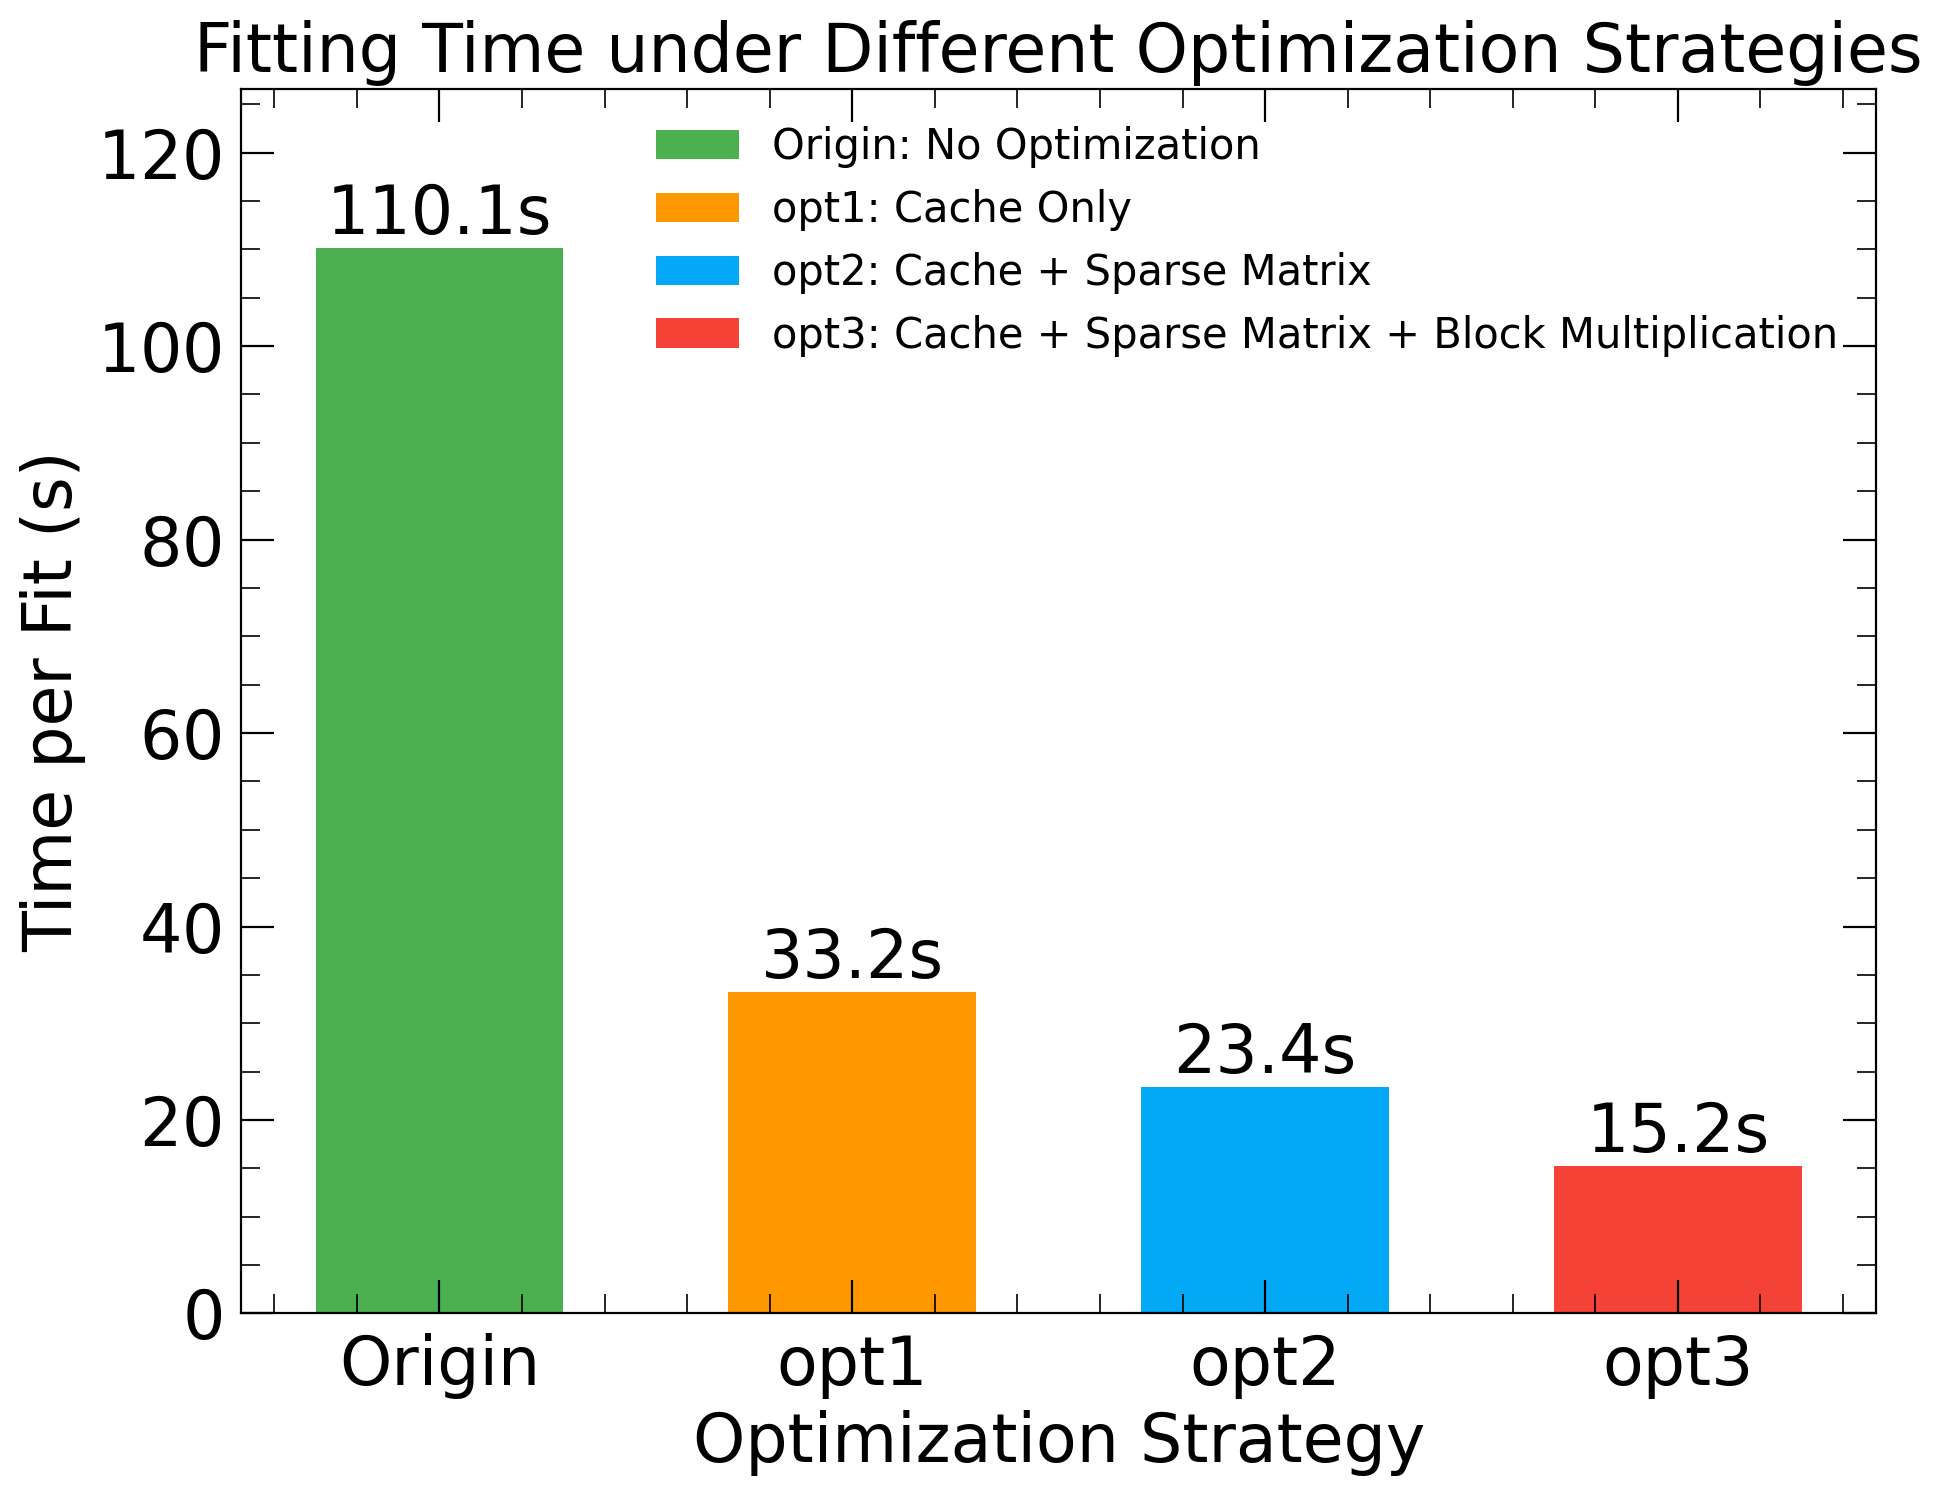
\includegraphics[width=0.6\textwidth]{Img/fitting_time_under_different_optimization_strategies.png}  
\bicaption{不同优化策略下单次拟合平均耗时比较。横坐标依次为：未经优化的基线实现（\textit{Origin}）、仅启用缓存（\textit{opt1}）、缓存 + 微分散射截面稀疏表示（\textit{opt2}）、缓存 + 稀疏表示 + 分块乘法（\textit{opt3}）。纵坐标为单次拟合的平均壁钟时间（秒）。柱状图展示了随着逐步应用优化策略，运行时间的逐级下降；其中 \textit{opt3} 达到最短的拟合时间。}{Comparison of average fitting time per fit under different optimization strategies. The horizontal axis lists the tested strategies: the baseline without optimization (\textit{Origin}), caching only (\textit{opt1}), caching with sparse matrix representation (\textit{opt2}), and caching with sparse matrix representation plus block multiplication (\textit{opt3}). The vertical axis shows the average wall-clock time in seconds required for a single fit. The bars illustrate the progressive reduction in runtime as successive optimizations are applied, with \textit{opt3} achieving the shortest fitting time.}  
\label{fig:fit_per_t_opt}  
\end{figure}

图~\ref{fig:computation_time_comparison_before_after_acceleration} 显示了针对关键模块的定量对比：在定点优化后，整体拟合性能显著提升。用于计算期望信号谱的时间由原来的 $108.6\ \mathrm{s}$ 降至 $14.3\ \mathrm{s}$，约为 $8\times$ 的加速。在谱计算内部的两大热点上，探测器响应矩阵的构造时间从 $72.4\ \mathrm{s}$ 缩短到 $8.1\ \mathrm{s}$（约 $9\times$ 加速），而沉积能量谱的计算（包括微分散射截面映射与矩阵乘法）则从 $33.4\ \mathrm{s}$ 缩短到 $5.0\ \mathrm{s}$（约 $6\times$ 加速）。其余次要任务时间变化甚微，不影响总体结论。

\begin{figure}[htbp]  
\centering  
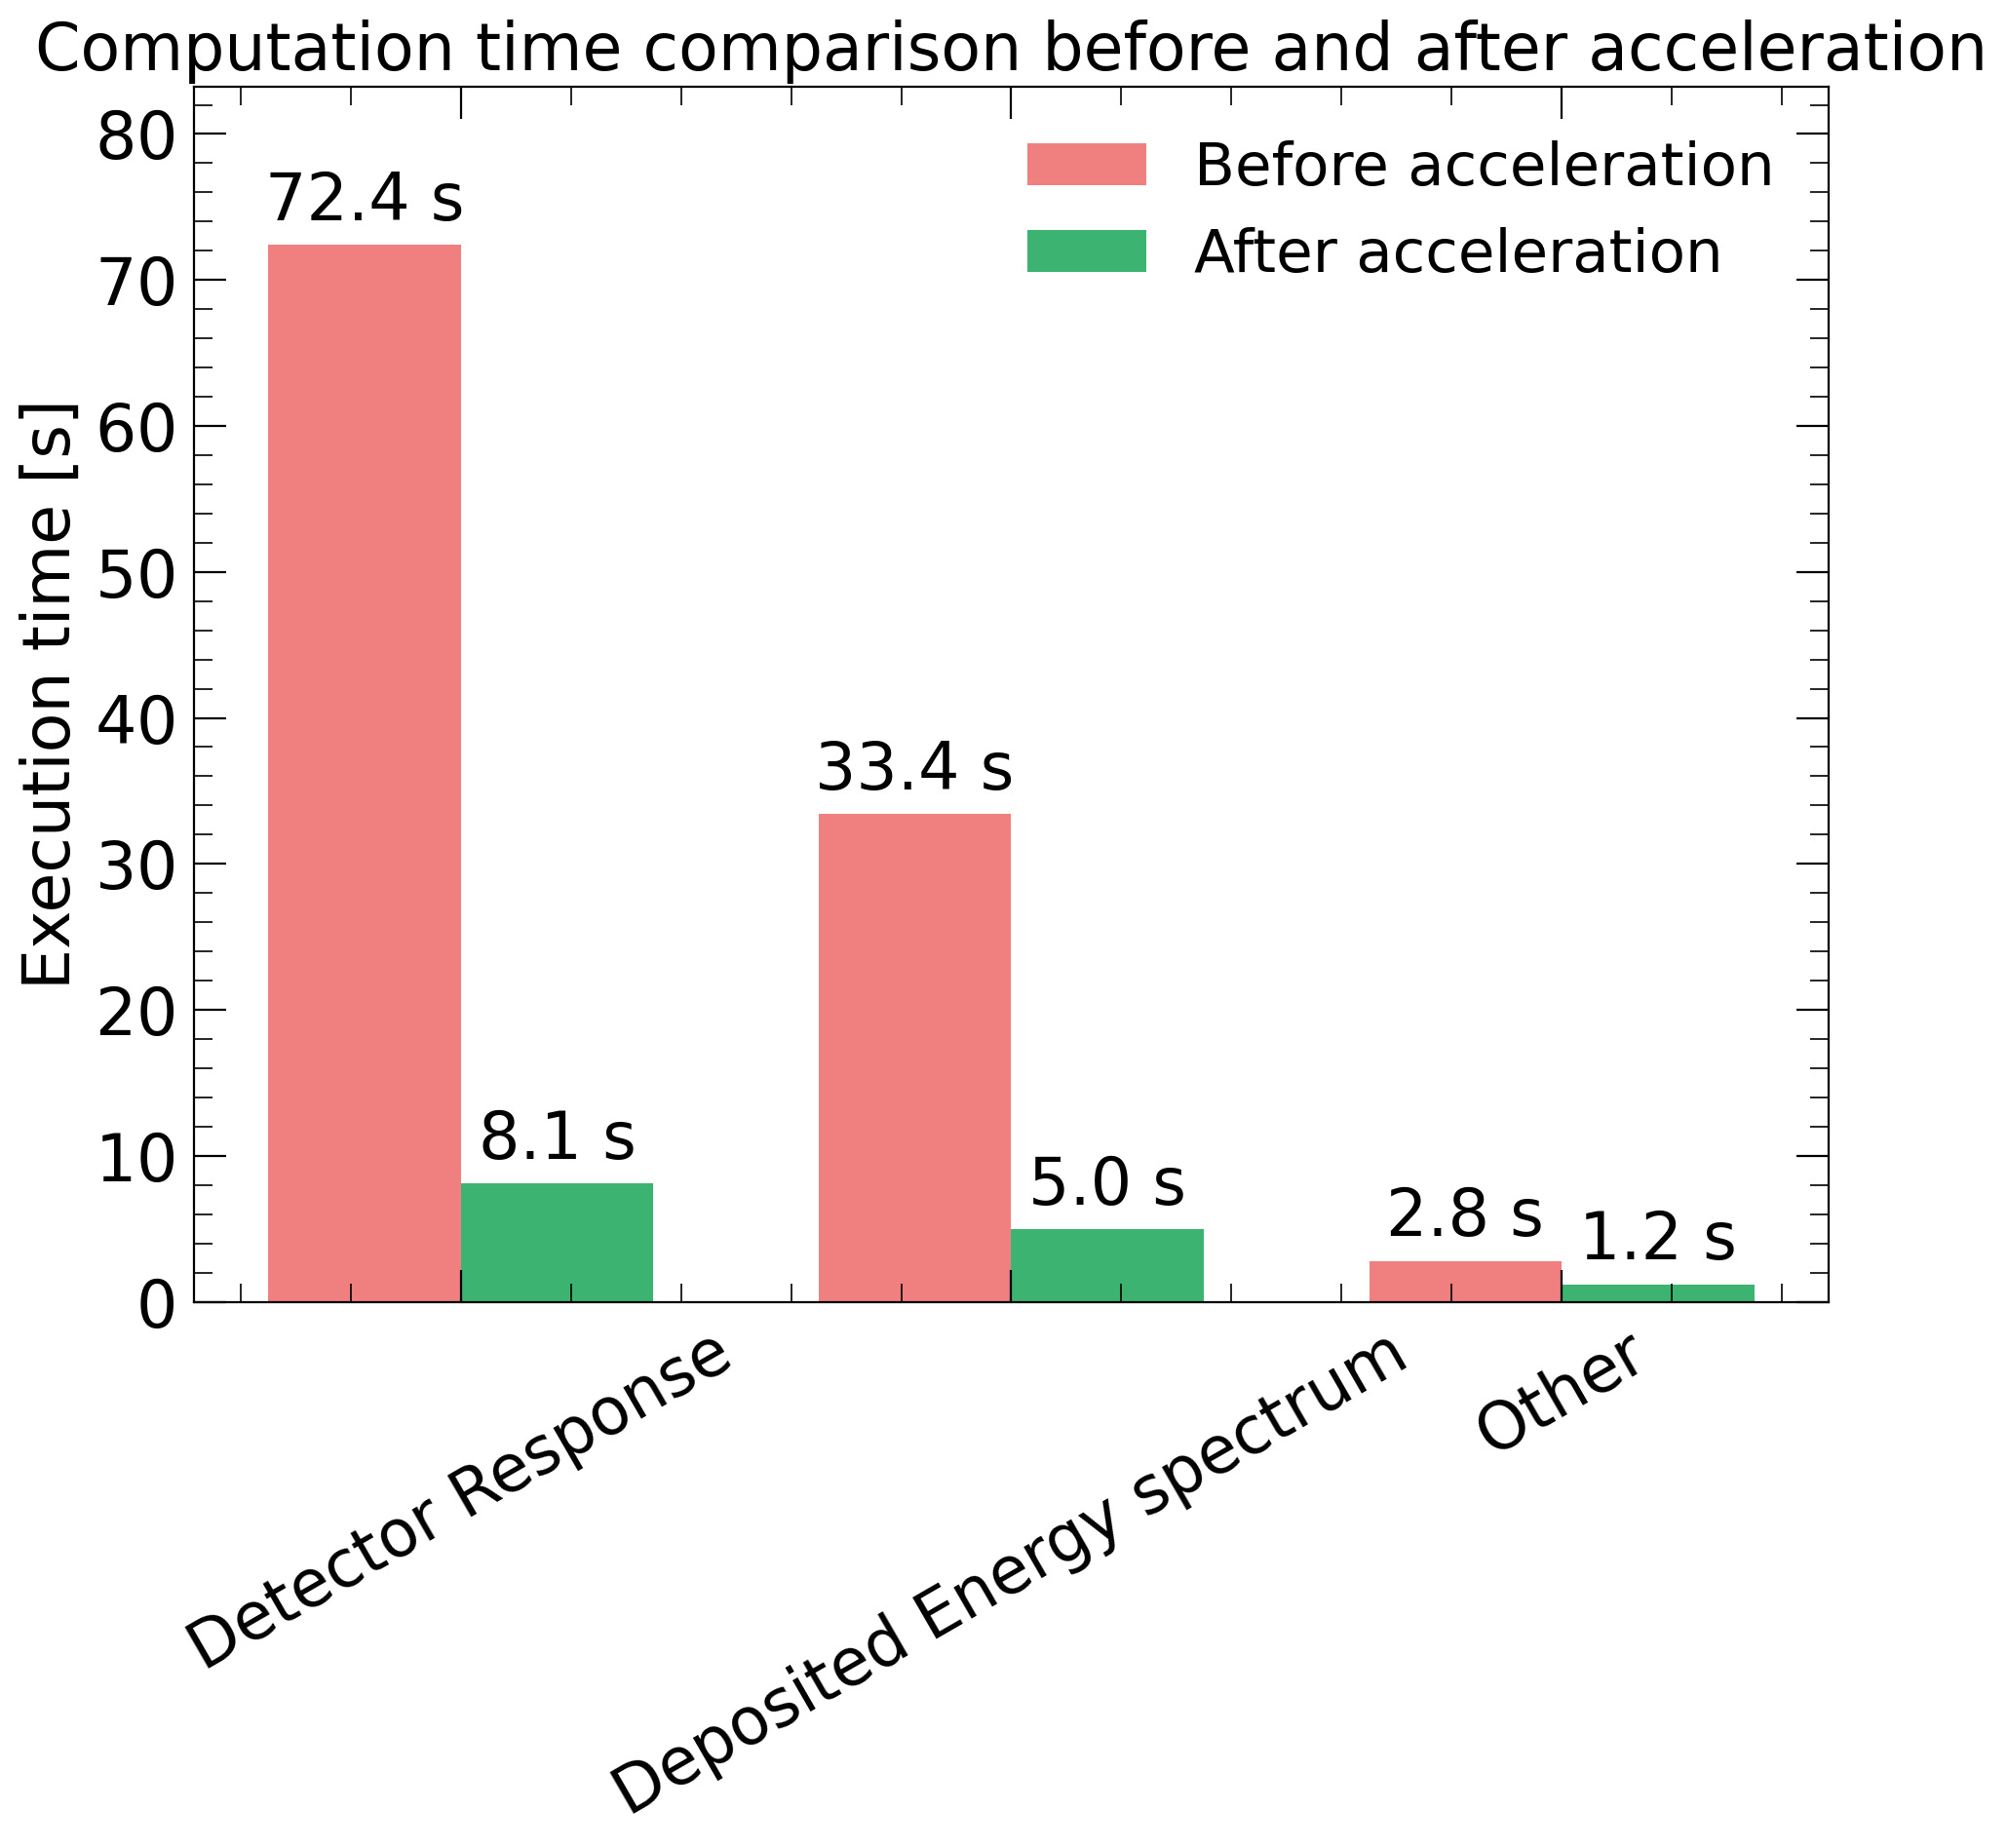
\includegraphics[width=0.6\textwidth]{Img/computation_time_comparison_before_after_acceleration.png}  
\bicaption{主要模块在应用加速技术前后的计算时间对比。图中显示探测器响应矩阵与沉积能量谱计算这两项主导性任务在加速后均获得显著缩短，从而推动整体拟合耗时的大幅下降。}{Computation-time comparison of major modules before and after acceleration. The dominant tasks—detector response matrix construction and deposited-energy spectrum calculation—are significantly reduced after optimization, leading to a large decrease in the overall fit time.}  
\label{fig:computation_time_comparison_before_after_acceleration}  
\end{figure}

综上所述，通过缓存、稀疏化与分块处理三类互补的工程与算法优化措施，我们在不牺牲拟合精度的前提下，实现了对能谱拟合的显著加速。该性能提升将使得原本因计算代价难以承受的大规模 Feldman–Cousins 覆盖性构造与广域 toy-MC 扫描变为可行，从而支持更严格的频率学置信区间验证与更全面的参数空间探索。

\subsection{能谱分箱对拟合耗时的影响}  
\label{sec:bin}

我们还研究了不同重建能量分箱数对总体拟合耗时的影响。固定重建能量观测区间为 $[0.8,\,12.0]$ MeV，分别将该区间等距划分为 $N_{\rm bin}=560,\;280,\;140,\;70,\;35$ 个箱，并在相同的优化策略下进行基准测试。图~\ref{fig:fit_time_per_bins} 给出了在若干优化配置下，单次完整拟合耗时随直方图 bin 宽变化的依赖关系。可以看到，在所有测试情形下，随着 bin 宽增大（即箱数减少），单次拟合耗时单调下降。其根本原因是：增大 bin 宽会减少重建能量能谱的箱数 $M$，从而缩小探测器响应矩阵的维度，降低每次似然评估所需的计算量。

我们考察的优化策略包括：缓存（caching）、微分散射截面稀疏（CSR）表示、以及分块（tiled）乘法/分块构造。缓存与稀疏表示在整个 bin 宽范围内均能稳定带来加速；而分块乘法在箱数较多（bin 宽较细、矩阵尺寸最大）时能显著提升性能，但当 bin 较粗时分块带来的优势会减小甚至消失。

在反应堆反中微子拟合中，探测器响应矩阵 $R$ 的构造与应用是主要的计算瓶颈之一。设 $R$ 的尺寸为 $M\times N$，其中 $M$ 为重建能量箱数，$N$ 为沉积能量箱数。每个矩阵元 $R_{ij}$ 都需通过高斯积分（误差函数 $\operatorname{erf}$）评估以得到相应的概率，因此直接构造完整矩阵的标量运算量可近似表示为

$$\text{Cost}_{\text{full}} \propto C \times M \times N,$$

其中常数 $C$ 表示构造每个元素所需的代价（包括若干次浮点减法、除法及一次 $\operatorname{erf}$ 计算）。忽略常数因子，总体计算复杂度规模为

$$T_{\text{full}}=\mathcal{O}(M\cdot N).$$

当增大重建或沉积能量能谱的 bin 宽（即降低分辨率）时，$M$ 或 $N$ 会相应下降；例如在固定区间 $[E_{\min},E_{\max}]$ 下，若将 bin 宽加倍，则箱数 $M$ 减半，总体计算量按线性比例缩减。

然而，当矩阵尺寸下降到足够小的阈值后，每个计算块已经足以完全驻留在 CPU 的缓存中，原先分块处理带来的缓存局部性优势将消失。同时，分块处理本身存在固定开销（函数调用、内存对齐与切片等），这些固定开销在单块计算量变小后会变得相对显著，从而抵消原先因改进局部性而得到的性能提升。因此，若箱数继续减小至某一临界点（即 bin 足够稀疏），分块方法的实际加速效应会趋近于零。

图中还标注了若干采样点的拟合迭代次数（所示点的注记），可见在不同 bin 宽下拟合器的迭代次数变化很小，这表明分箱选择主要影响的是每次迭代的计算成本，而不是最小化算法的收敛行为。

综上所述，较细的分箱会显著增大探测器响应矩阵的规模和每次迭代的计算量，使得采用先进的加速策略（如缓存、稀疏化与分块化）成为保持可接受拟合时间的必要手段；而对于较粗的分箱，矩阵尺寸天然变小，单次计算成本降低，使得分块矩阵乘法等性能优化的效果下降。

\begin{figure}[htbp]  
\centering  
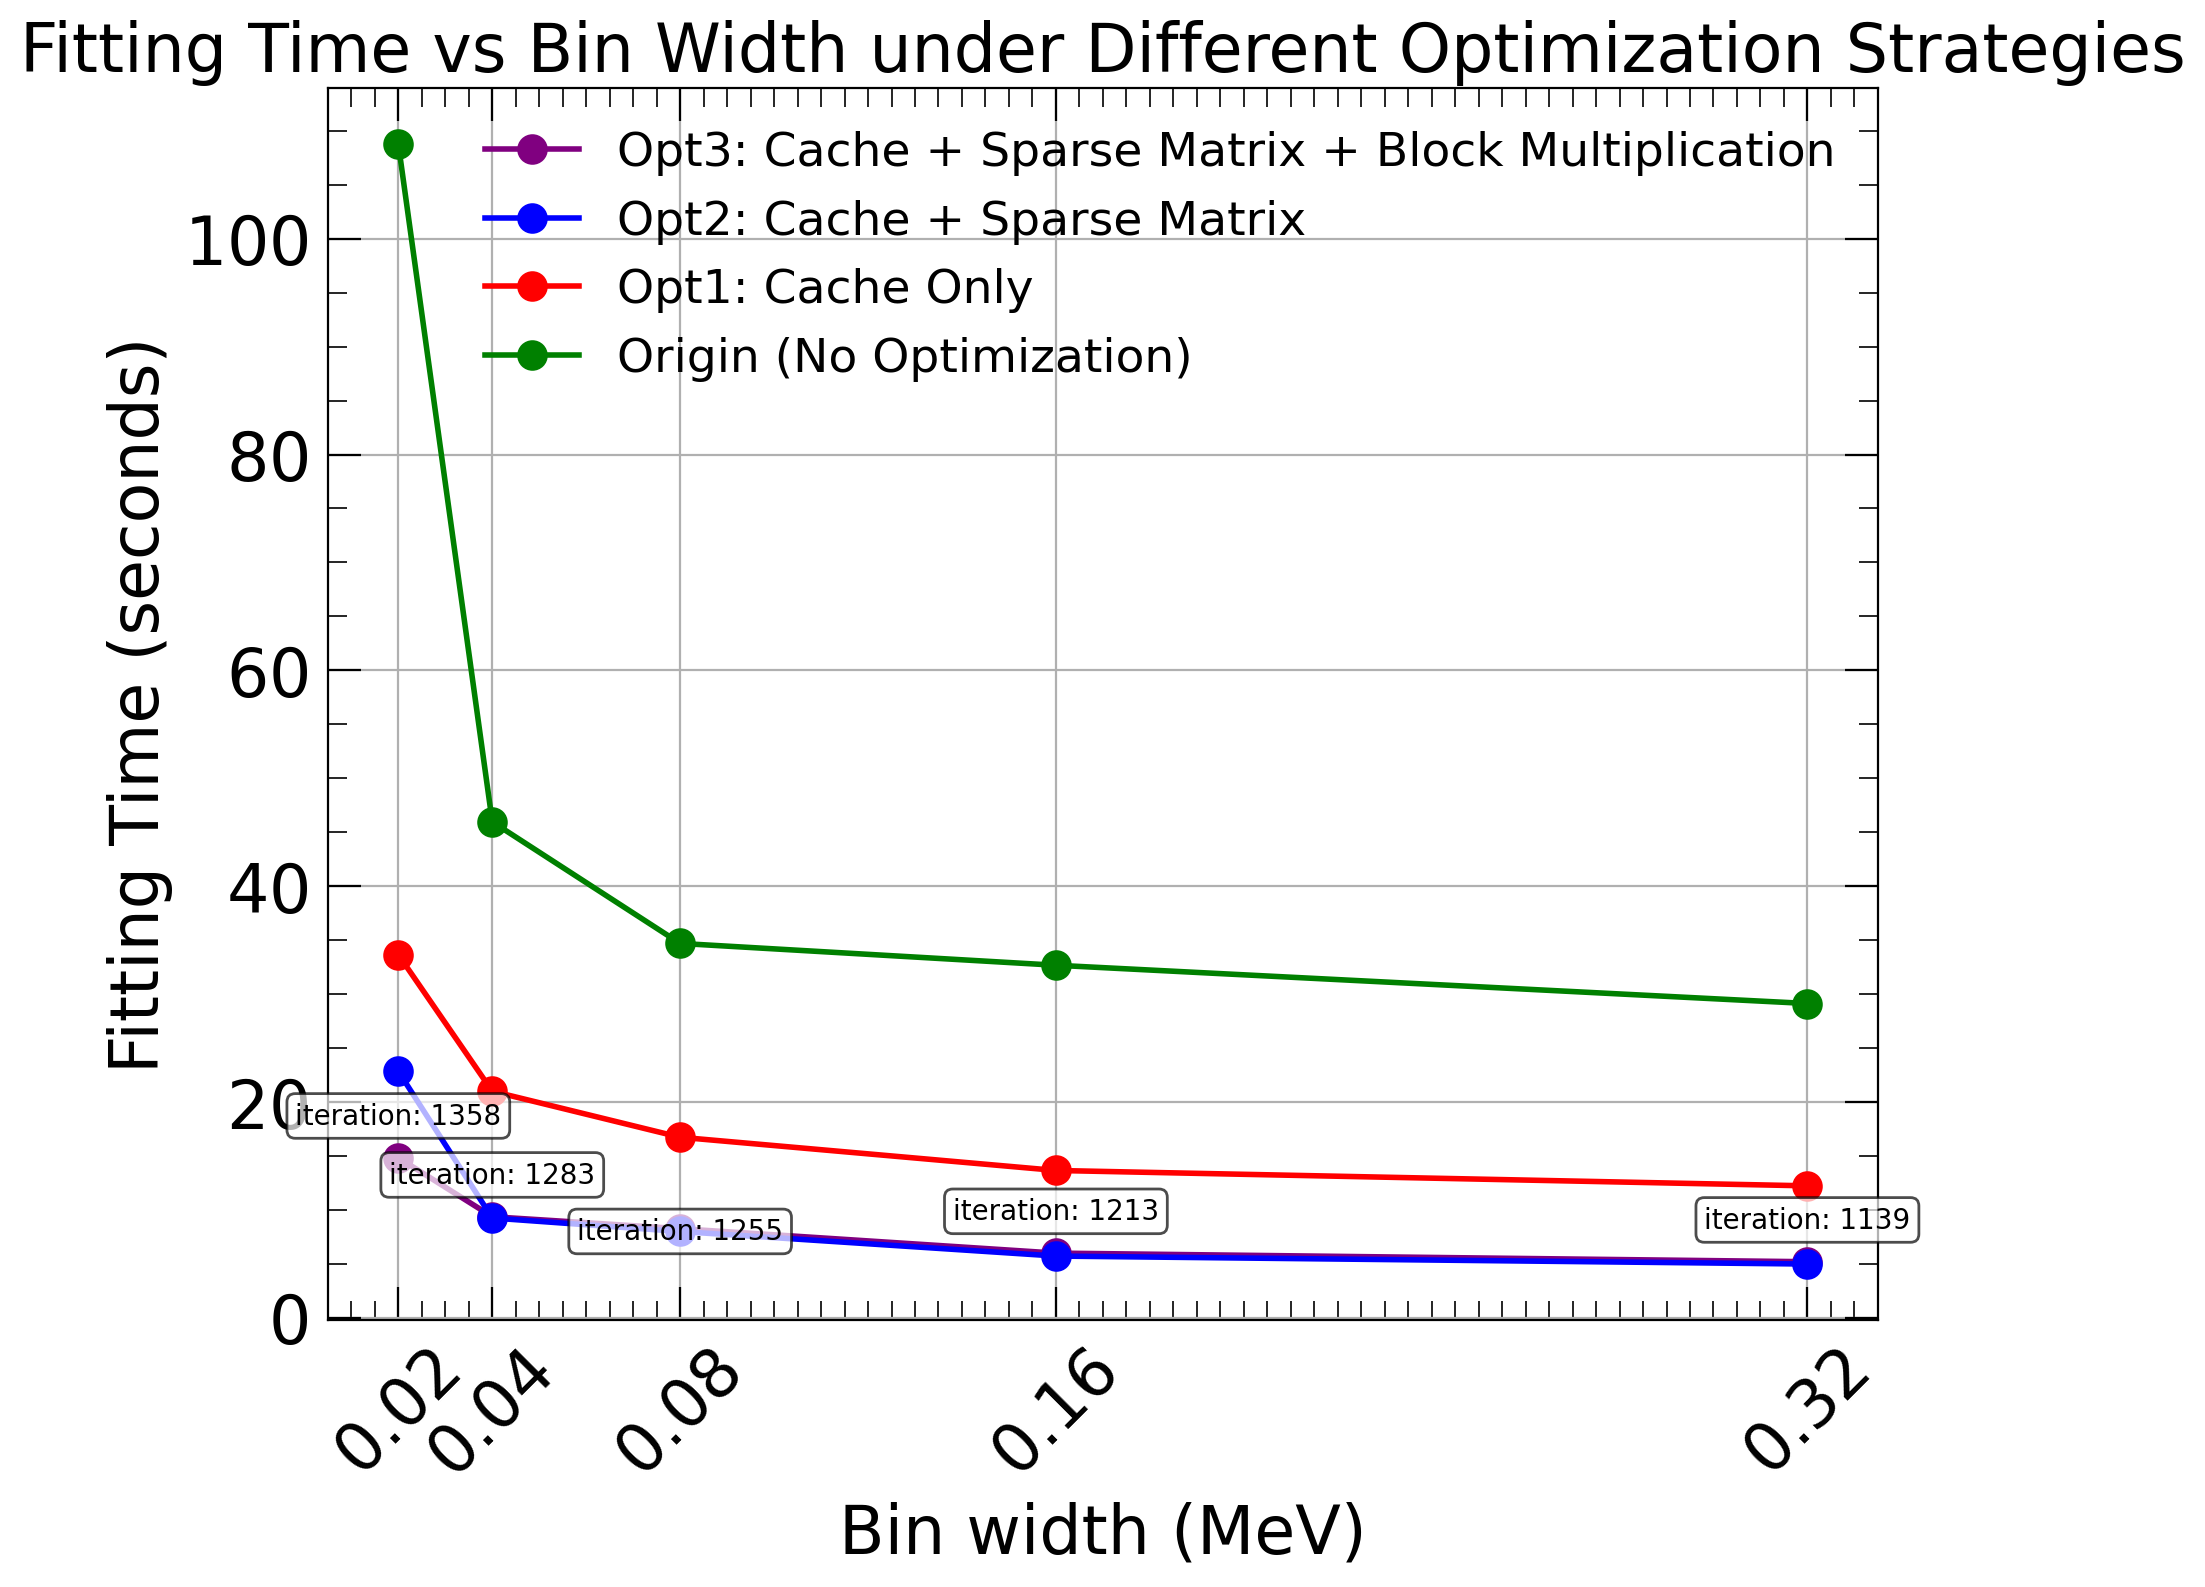
\includegraphics[width=0.6\textwidth]{Img/fitting_time_vs_bin_width.png}  
\bicaption{单次完整拟合耗时随重建能量能谱 bin 宽的变化。横轴为重建能量能谱直方图的 bin 宽（MeV）；纵轴为单次完整拟合的时间（秒）。曲线对应不同的优化配置：绿色 — 基线（无优化）；红色 — 仅缓存；蓝色 — 缓存 + 稀疏（CSR）存储；品红色 — 缓存 + 稀疏 + 分块（tiled）乘法。每个点均在相同的能量区间 $[0.8,\,12.0]$ MeV 下通过不同等距箱数计算得到。}{Fitting time as a function of reconstruction-bin width. The horizontal axis shows the bin width of the reconstructed-energy histogram (MeV); the vertical axis gives the total wall-clock fitting time (s) for a single full fit. Curves correspond to different optimization configurations: green — baseline (no optimization); red — caching only; blue — caching + sparse (CSR) matrix storage; magenta — caching + sparse matrix + block (tiled) matrix multiplication. Each point was obtained for the same reconstructed-energy interval ([0.8, 12.0] MeV) but with different numbers of uniform bins (equivalently different bin widths).}  
\label{fig:fit_time_per_bins}  
\end{figure}

\section{本章小结}
\label{sec:ch3_summary}
本章内容提出的多项加速技术在保证数值精度的前提下，显著提升了反应堆反中微子能谱拟合的计算效率。具体而言：

首先，通过缓存（caching）策略将拟合过程中频繁重复出现的中间计算结果保存并复用，避免了大量冗余计算。基准测试表明，仅启用缓存即可将拟合速度提高约 $3\times$。

其次，充分利用微分散射截面矩阵与响应矩阵的带状稀疏性，将这类矩阵以压缩稀疏格式（如 CSR）存储，并仅对非零元执行计算，从而大幅减少乘加运算与内存访问。我们的测试显示，这一稀疏化处理带来了约 $1.5\times$ 的加速。

再次，通过对探测器响应矩阵采用分块（blocked / tiled）乘法与逐块构造的方法，可改善数据局部性并降低内存搬运开销。该方法在我们的实现中同样贡献了约 $1.5\times$ 的加速。

将上述三类技术组合后，相较于未经优化的实现，总体拟合耗时在本测试环境下缩短了约 $7\times$。

我们还量化了重建能量分箱对计算耗时的影响。增大 bin 宽（即减少箱数）会直接缩小响应矩阵的维度，从而使每次似然/χ²评估的计算成本按矩阵规模近似线性下降；在我们的测试中，最小化器迭代次数基本保持不变，因此总耗时主要受每次迭代的计算代价驱动。由此可见，在分辨率与计算开销之间存在明显的权衡：极细的分箱会增加矩阵规模，这时分块乘法的加速效果最优；而缓存与稀疏存储在广泛的分箱设置下均能提供稳健的加速效果。

总体而言，本工作所采用的缓存、稀疏化与分块等互补性优化措施，大幅降低了重建能量能谱拟合的计算代价，构建了一个高效且可扩展的前向折叠（forward-folding）加速框架。该方法对当前与未来的中微子实验（例如 JUNO、Hyper-Kamiokande、DUNE 等）具有广泛适用性，有助于开启更大规模的 toy-MC 研究、更快速的参数扫描以及更可行的频率学置信带（Feldman–Cousins）构造。



%=====================================================================
\chapter{JUNO实验能谱分bin策略}
%=====================================================================
在反应堆反中微子振荡分析中，能谱的分bin策略既是统计问题也是物理问题——不同的分箱尺度会改变单个 bin 的统计属性、影响谱形信息的保留程度，并进而影响振荡参数估计的偏差与精度。本部分首先明确两个必须区分的能谱概念：一是探测器层面的重建能谱（reconstructed-energy spectrum），即把沉积能量通过能量响应与重构程序得到的、用于拟合的观测直方图；二是物理层面的反应堆中微子能谱（reactor $\bar\nu_e$ spectrum），即裂变同位素在反应堆中产生的原始入射通量及其模型化表达。两类能谱的分bin选择各有侧重点：重建能谱的分bin决定了观测统计与似然近似的有效性；反应堆能谱的分段决定了模型依赖性与外场约束（如来自 Daya Bay 的近场测量）能否有效抑制谱形不确定性。

具体地，重建能谱在低统计量条件下如果使用过细的分箱，会导致若干边缘箱（尤其是谱尾或窄能区）内事件数过小，从而违背常用高斯近似的前提。当基于高斯近似构造 χ² 或直接套用 Wilks 定理来估计置信区间时，这类近似失效会引入系统性偏差，甚至导致置信区间的覆盖率不正确。相对地，反应堆中微子能谱的分段若过细，所定义的谱形自由度可能超出近点探测器实验（Daya Bay reactor neutrino experiment）提供的约束能力，使得拟合对反应堆模型的依赖性增强，从而在不同模型假设下产生可观的系统误差。因此，分箱策略必须在“保留谱形细节以维持灵敏度”与“避免统计近似失效及模型依赖过强”之间找到平衡点。

为了解决上述矛盾并给出可操作的建议，本部分将采用定量化方法：一方面通过大量 toy-MC 实验评估在不同重建能谱分箱下（从非常细到较粗）振荡参数估计的偏差与覆盖率，比较基于高斯近似（CNP,Pearson）与基于泊松似然的统计量在低统计情形下的表现；另一方面构造两类反应堆谱情形——一个为固定反应堆模型（fiducial spectrum），另一个为包含小幅谱形扰动的变化模型（model variation），在不同反应堆能谱分段尺度下比较拟合的精度与由模型依赖引入的系统误差。通过这种“固定-扰动”对比实验，我们将量化在何种中微子能谱分段尺度下，反应堆模型依赖对关键振荡参数（如 $\Delta m^2$）的影响可被接受，从而给出实验可采纳的分bin建议。
本章研究的成果被江门中微子实验合作组采用，并应用与第一篇物理文章的振荡分析中。本章的组织如下：第1节介绍重建能谱的分bin策略；第二节介绍反应堆能谱的分bin策略。

\section{重建能谱分bin策略与低统计量下太阳振荡参数的测量}
本节讨论在低统计量条件下对太阳中微子振荡参数 $\Delta m^2_{21}$ 和 $\sin^2\theta_{12}$ 的测量。我们首先生成5000个伪实验数据集，振荡参数和系统学参数均取名义值，并同时包含统计涨落和系统误差涨落。然后，我们比较基于高斯近似（CNP,Pearson）与基于泊松似然的统计量在低统计情形下的表现。最后，我们给出在不同重建能谱分bin策略下，太阳振荡参数的偏差与精度。

生成 toy 数据所使用的配置与~\ref{sec:Arrived neutrino spectrum}中相同。特别地，在以下结果中，我们对 Asimov 数据以及伪实验均采用组合的 Pearson–Neyman 统计量 $\chi^2_{\mathrm{CNP}}$，这种选择旨在减小振荡参数估计中的偏差。

最后，在相同的伪实验集合下，我们考察了不同重建能谱分 bin 策略对太阳振荡参数偏差（bias）与测量精度（precision）的影响。通过比较各分 bin 方案下的拟合输出分布、均值偏差与置信区间宽度，能够定量判断在早期低统计阶段采用何种分 bin 策略可在保持统计灵敏度的同时尽量抑制由高斯近似失效或低统计量引起的系统性偏差。
\subsection{Toy MC 研究}

在多个曝光时间下，生成了5000个伪实验数据集。振荡参数和系统学参数均取名义值，并同时包含统计涨落和系统误差涨落。

\begin{figure}[ht]
    \centering
    \begin{subfigure}[t]{0.47\textwidth}
      \centering
      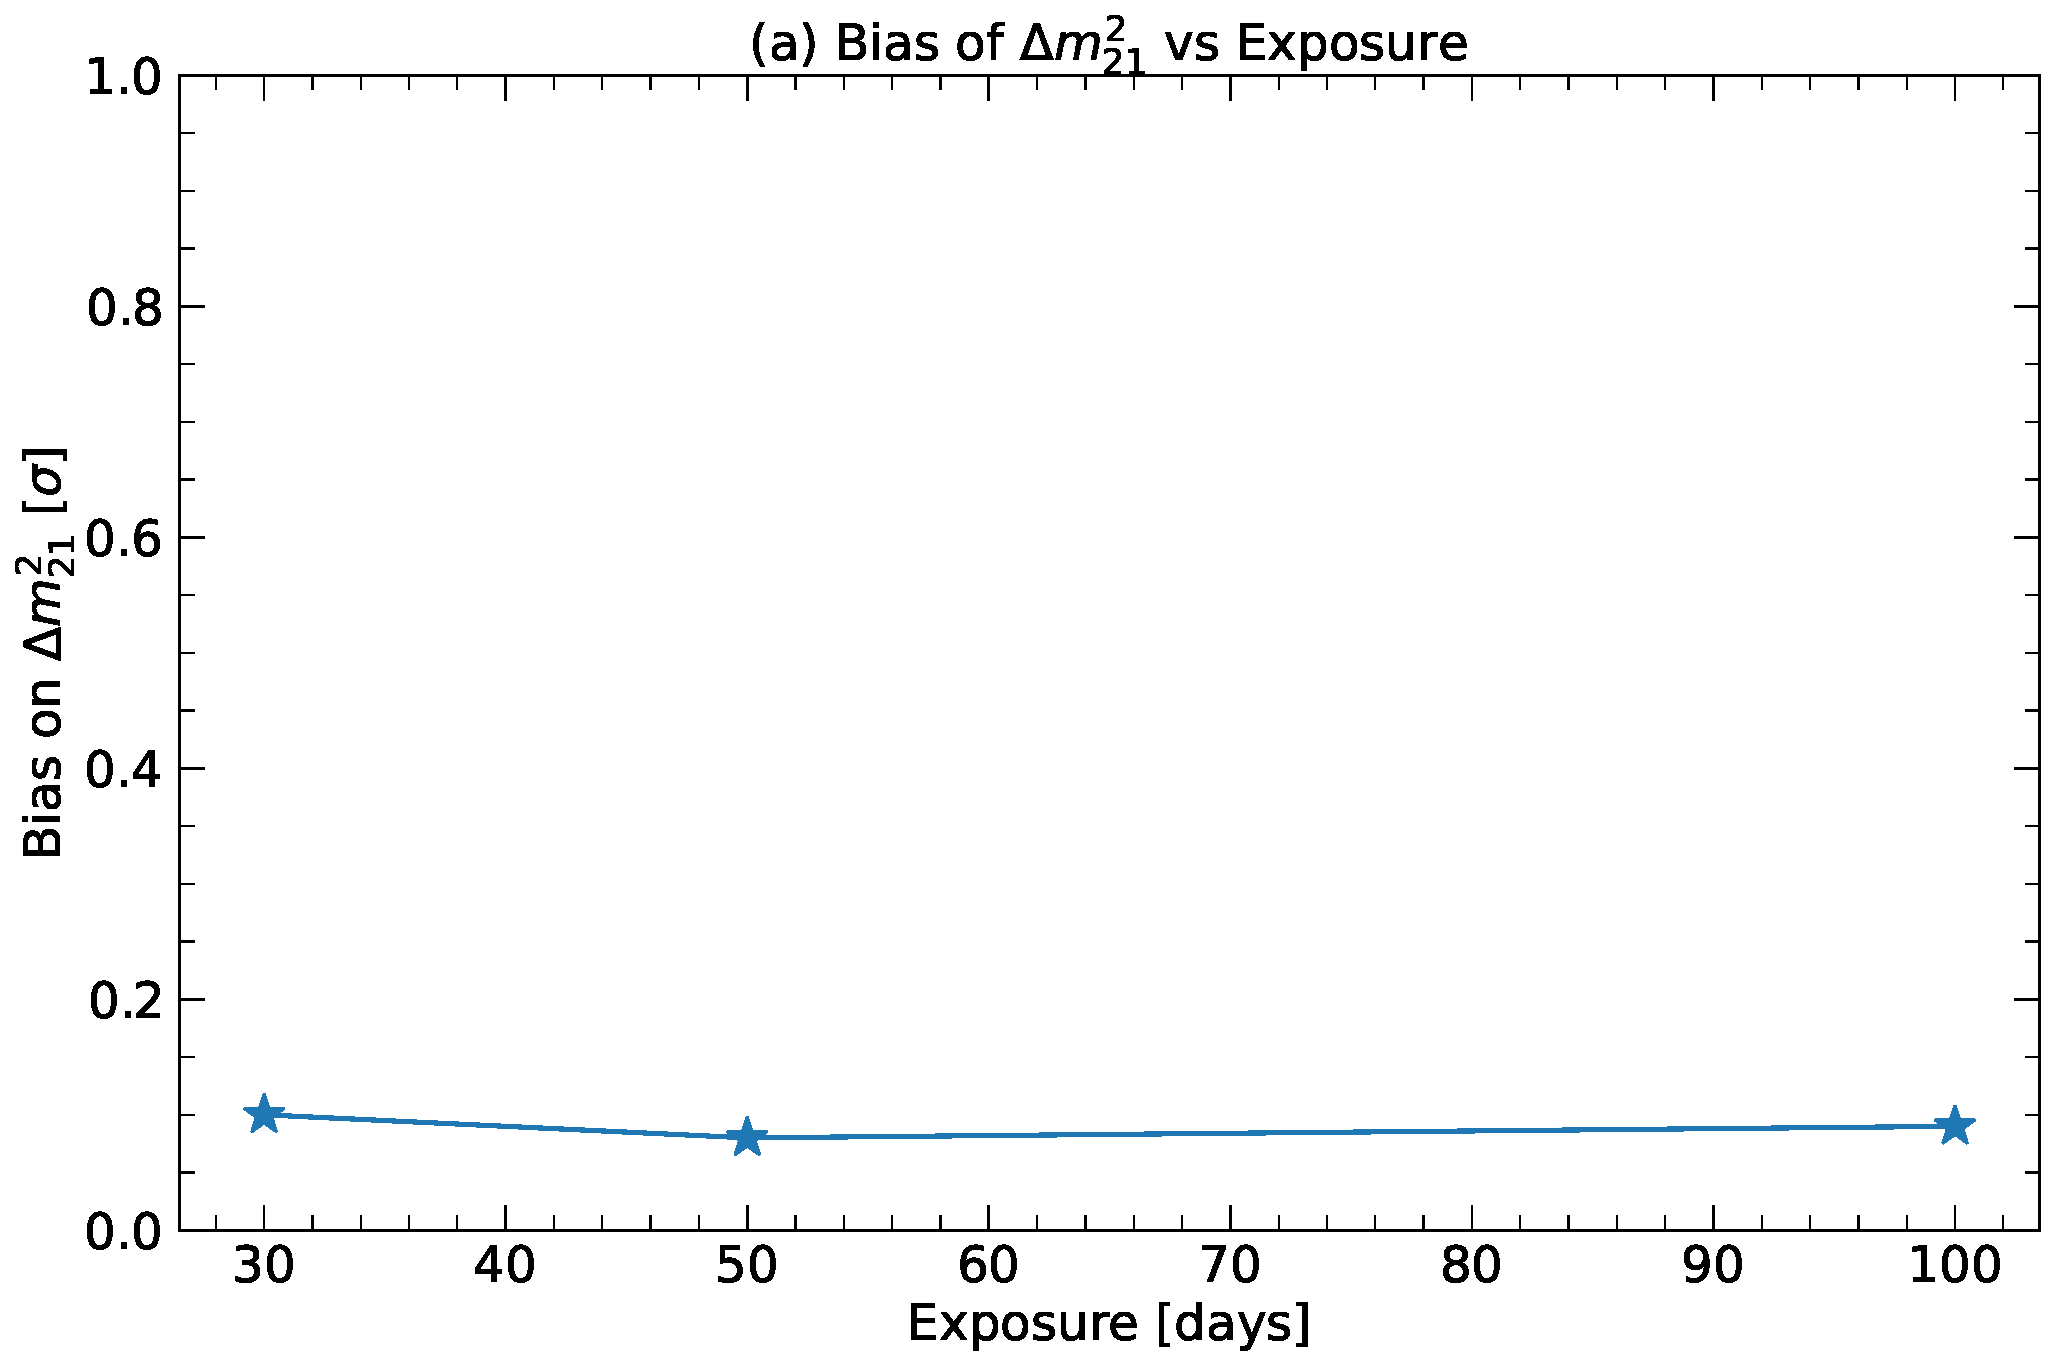
\includegraphics[width=\linewidth]{Img/binning strategy/Bias_of_dm21_vs_exposure.pdf}
      \caption{$\Delta m^2_{21}$ 偏差随时间的变化.}
      \label{fig:dm2_21_bias}
    \end{subfigure}
    \hfill
    \begin{subfigure}[t]{0.47\textwidth}
      \centering
      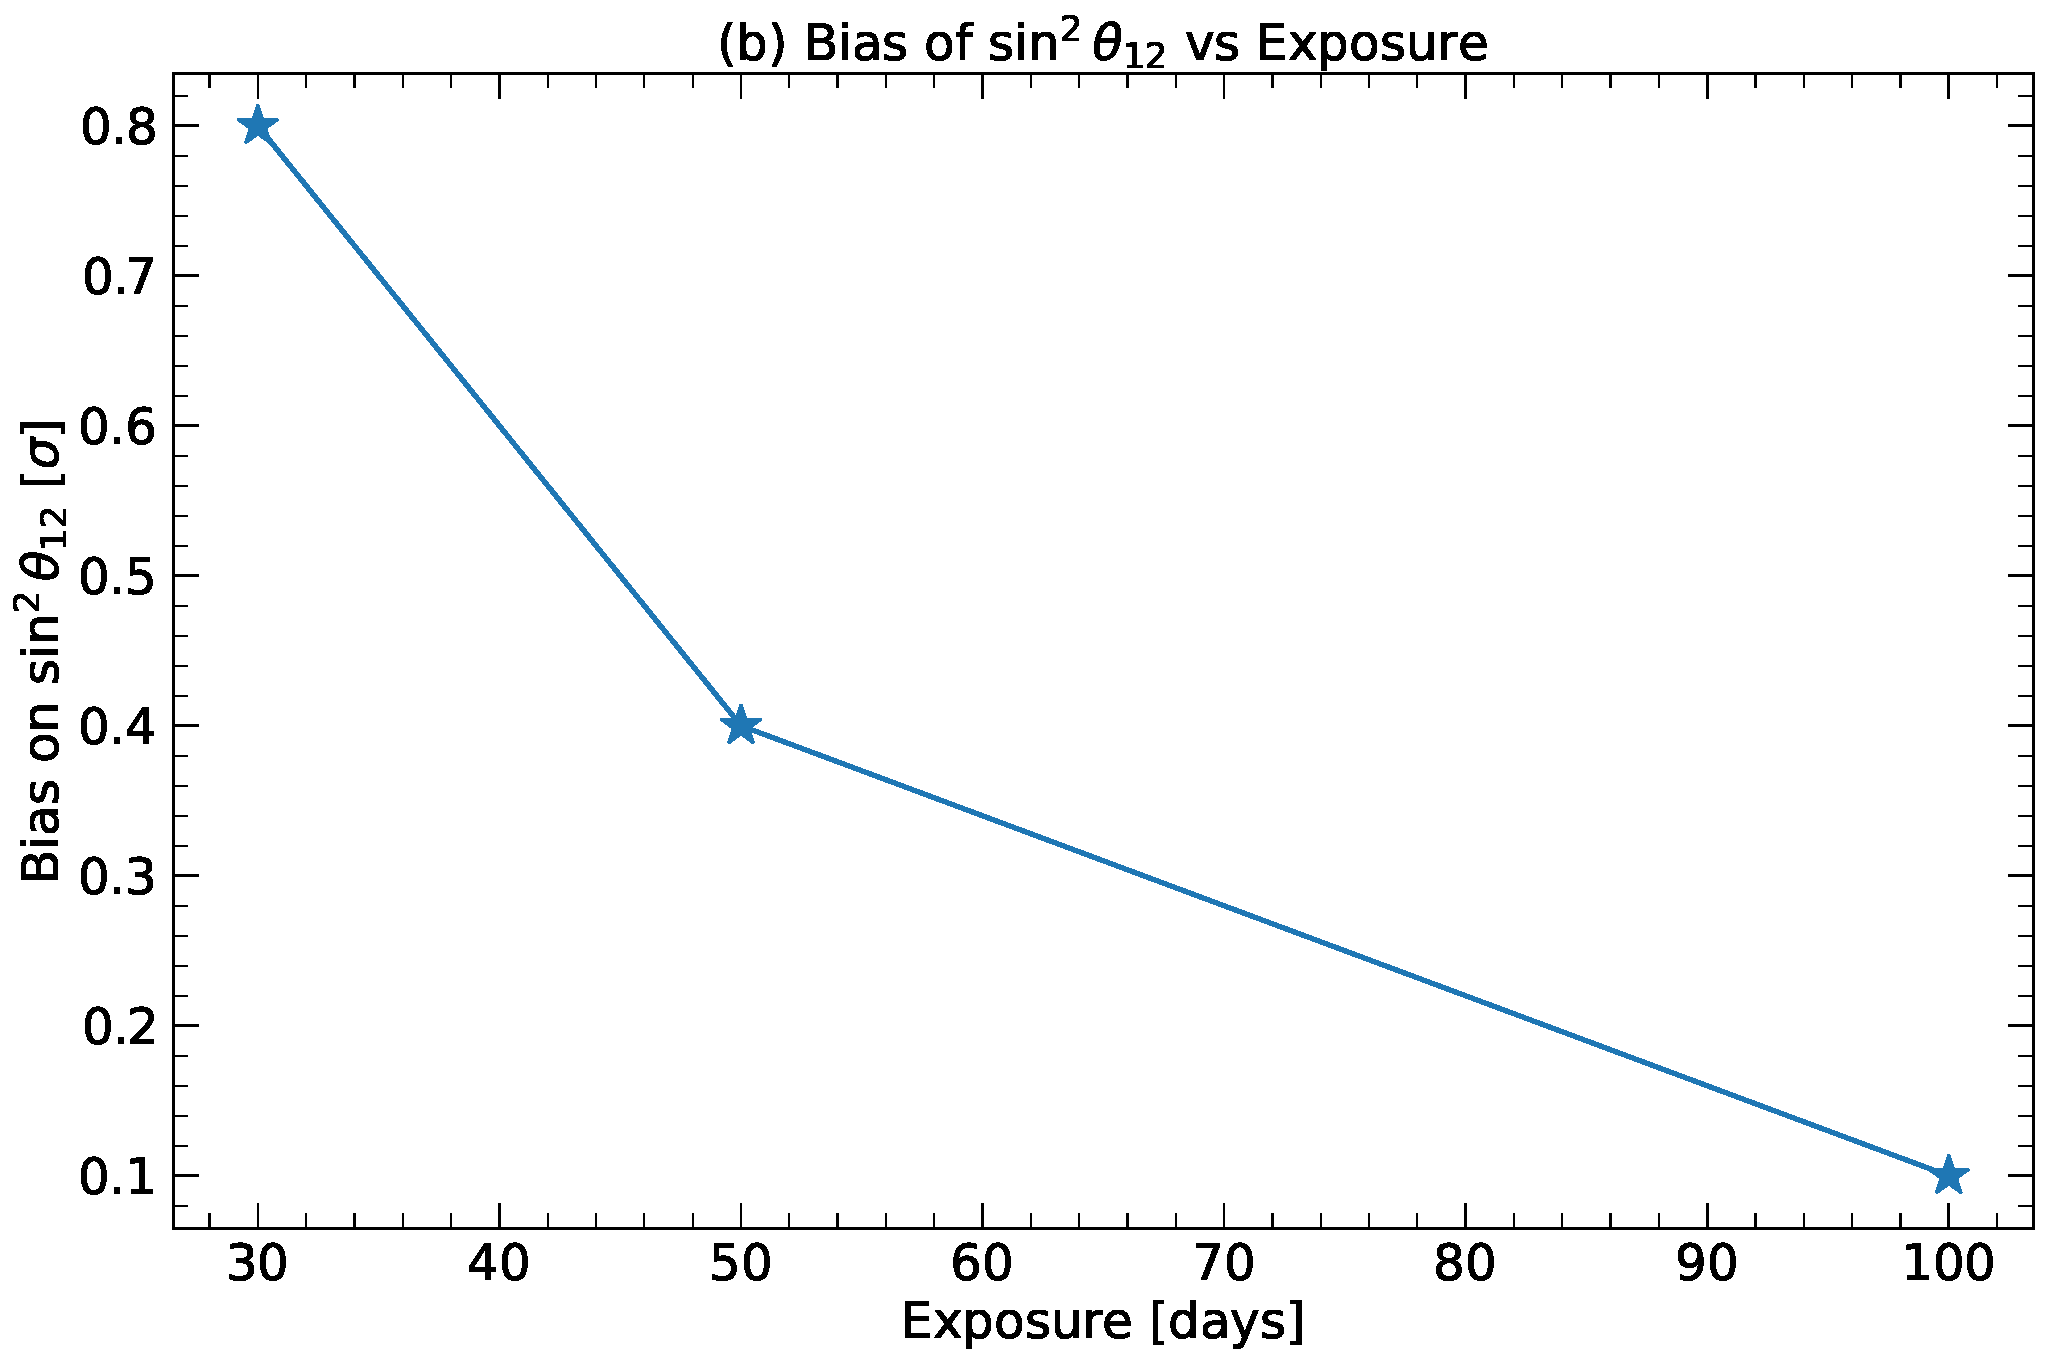
\includegraphics[width=\linewidth]{Img/binning strategy/Bias_of_sin2theta12_vs_exposure.pdf}
      \caption{$\sin^2\theta_{12}$ 偏差随时间的变化.}
      \label{fig:s12_bias}
    \end{subfigure}
    \bicaption{太阳振荡参数偏差随曝光时间的演化。（a）$\Delta m^2_{21}$ 的偏差；（b）$\sin^2\theta_{12}$ 的偏差。}
    {Evolution of the bias of solar oscillation parameters as a function of exposure time. Panel (a) shows the bias of $\Delta m^2_{21}$; panel (b) shows the bias of $\sin^2\theta_{12}$.}
    \label{fig:solar_low_stat_bias}
  \end{figure}
  
图~\ref{fig:solar_low_stat_bias} 给出了两类太阳振荡参数随暴露时间演化的偏差行为：\autoref{fig:dm2_21_bias} 展示了在 30 天、50 天和 100 天曝光条件下 $\Delta m^2_{21}$ 偏差随时间的变化；\autoref{fig:s12_bias} 展示了在 30 天、50 天和 100 天曝光条件下 $\sin^2\theta_{12}$ 偏差随时间的变化。Toy MC 结果与 Asimov 结果进行了比较。蓝色标记表示使用对称 68.27\% 积分法得到的置信区间：即将所有最佳拟合值按升序排列，然后计算分布的第 16 百分位和第 84 百分位。紫色标记与曲线来自对具有相同输入参数的 Asimov 数据集的拟合结果，其最佳拟合值及不确定度由最小化算法给出，并假设服从理想高斯分布。可以看出低统计量下太阳振荡参数存在显著偏差，但随着取数时间增加，偏差明显变小。此外，正如下文所讨论的，采用不同的分 bin 策略可以进一步减小这一效应。


\subsection{偏差与精度的演化}

在低统计数据条件下，谱中的某些 bin 可能只包含极少的事例，甚至没有事例。在这种情况下，χ² 检验统计量会变得不可靠，从而可能在参数估计中引入偏差。减少偏差的一种实际方法是在预期事件数较少的能区，或在整个分析范围内使用更宽的 bin。改变 bin 宽度的影响将在 \autoref{sec:binning_solar} 中进行研究。以下结果均基于名义分 bin，即 20 keV 宽度。

每个参数的偏差定义为最佳拟合值分布的平均值与真实输入值之间的归一化差异：

$$\text{Bias} = \frac{\langle\hat{\theta}\rangle - \theta_{\text{true}}}{\sigma_{\text{68\%}}},$$

其中，$\langle\hat{\theta}\rangle$ 表示5000个伪实验中最佳拟合值的平均值，$\theta_{\text{true}}$ 为名义输入参数值，$\sigma_{68\%}$ 为由上述分布估计得到的不确定度。

\autoref{fig:solar_low_stat_bias} 显示，两种太阳振荡参数在偏差行为上存在差异。对于 $\Delta m^2_{21}$，在所有曝光水平下偏差始终小于 $0.1\sigma$。相比之下，$\sin^2\theta_{12}$ 在 30 天曝光时表现出约 $0.8\sigma$ 的明显偏差，但随着取数时间增加，该偏差显著减小。


需要指出的是，上述结果是在系统误差取名义值的假设下得到的，即假设对系统学参数具有良好的控制。在实际情况下，仅凭 50 天数据难以实现对系统误差（如探测器响应、背景估计等）的如此精确控制。

\subsection{分 bin 策略}\label{sec:binning_solar}

\begin{figure}[h!]
    \centering
    \begin{subfigure}[t]{0.32\textwidth}
      \centering
      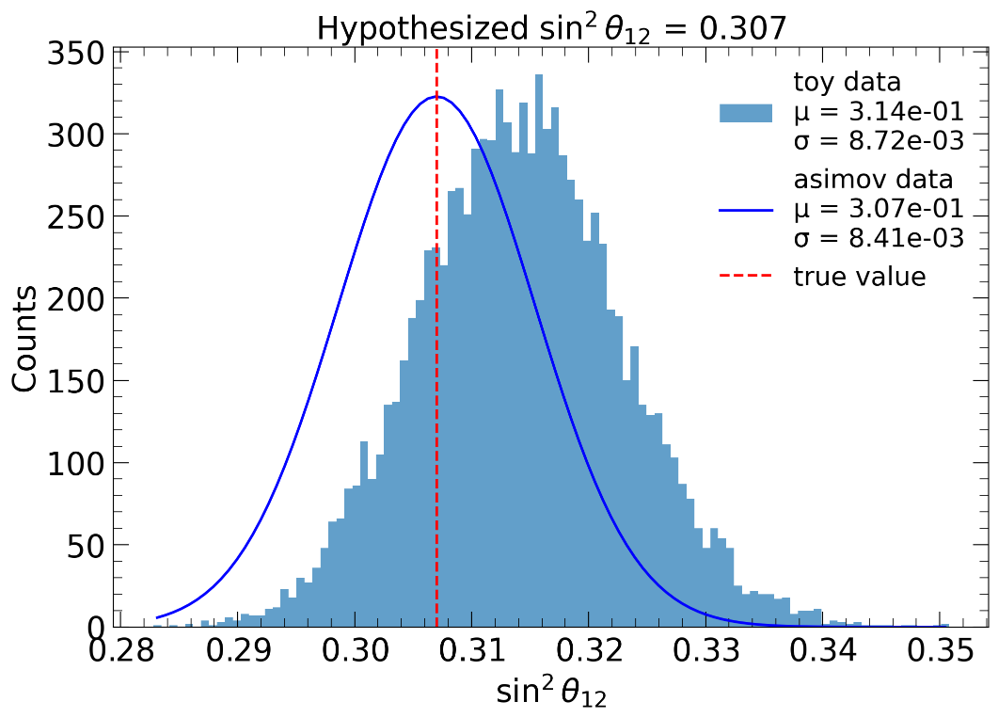
\includegraphics[width=\linewidth]{Img/binning strategy/Jingqin_sinsq12_bias_560bins.png}
      \caption{560 bins.}
      \label{fig:s12_binning_nominal}
    \end{subfigure}
    \hfill
    \begin{subfigure}[t]{0.32\textwidth}
      \centering
      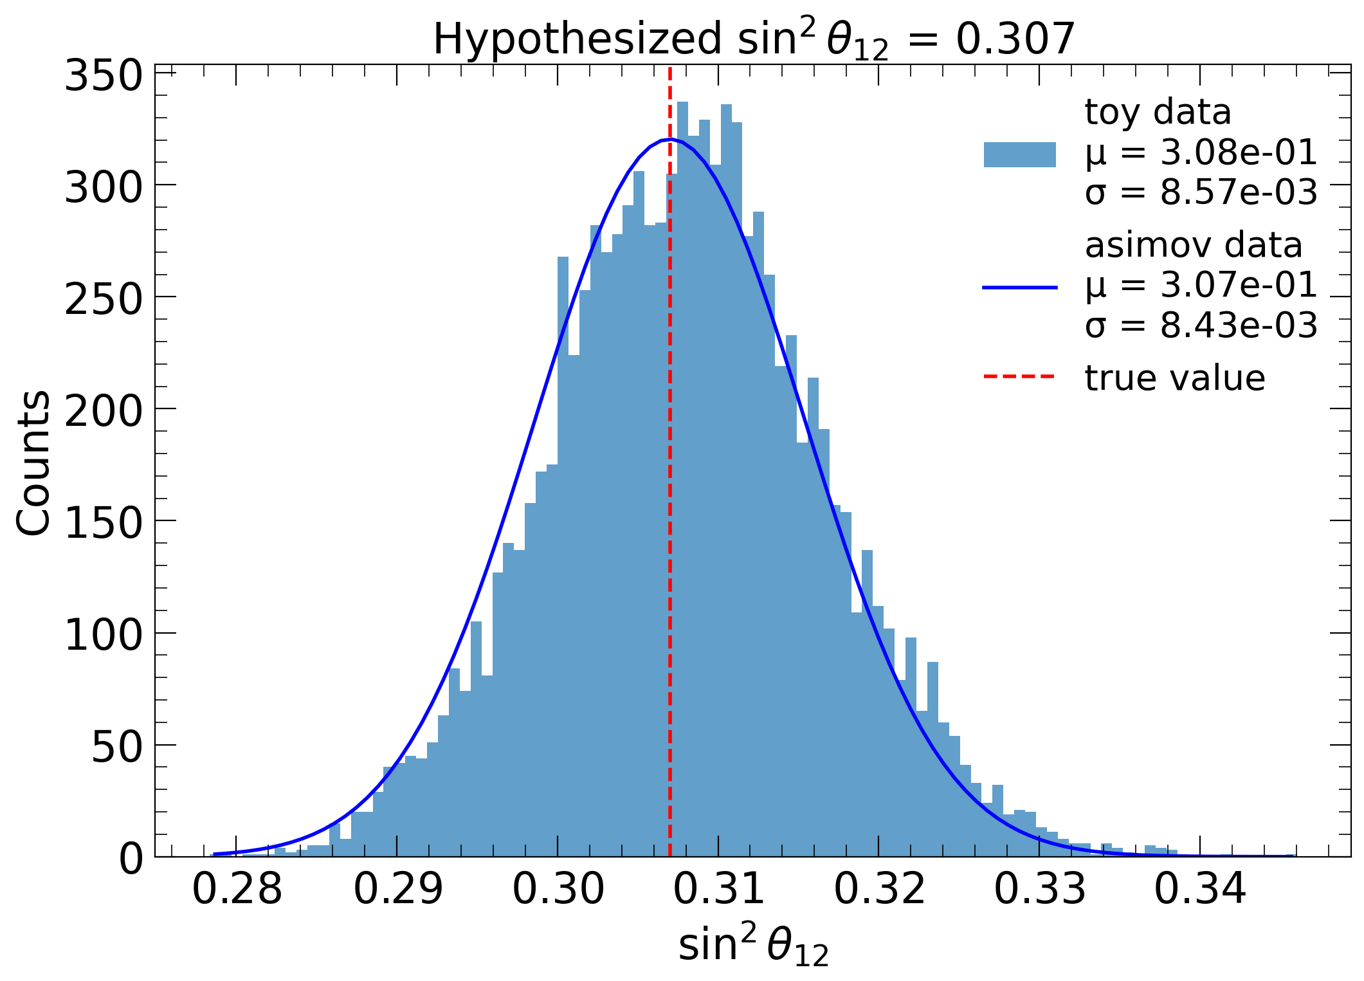
\includegraphics[width=\linewidth]{Img/binning strategy/Jingqin_sinsq12_bias_80bins.png}
      \caption{80 bins.}
      \label{fig:s12_binning_factor7}
    \end{subfigure}
    \hfill
    \begin{subfigure}[t]{0.32\textwidth}
      \centering
      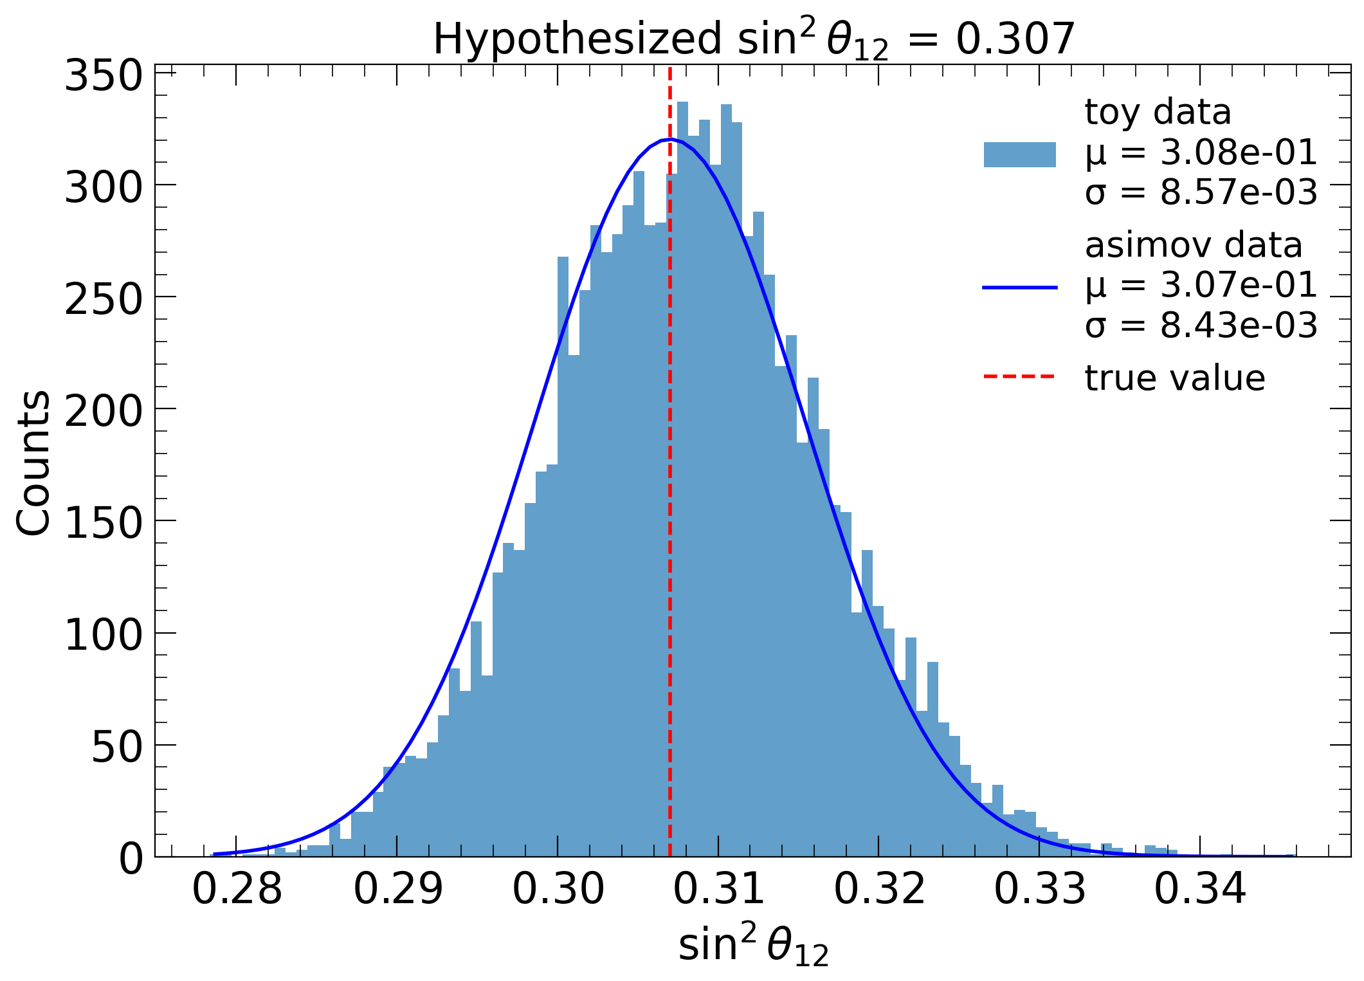
\includegraphics[width=\linewidth]{Img/binning strategy/Jingqin_sinsq12_bias_56bins.png}
      \caption{56 bins.}
      \label{fig:s12_binning_factor10}
    \end{subfigure}
    \bicaption
    {在 30 天曝光条件下，不同重建能谱分 bin 数目下 $\sin^2\theta_{12}$ 最佳拟合值在 10,000 个伪实验中的分布。}
    {Distribution of the best-fit values of $\sin^2\theta_{12}$ from 10,000 pseudo-experiments at 30 days exposure with different numbers of reconstructed energy bins.}
    \label{fig:s12_binning}
  \end{figure}

为研究并减小观测到的偏差，特别是在低曝光（30 天）条件下 $\sin^2\theta_{12}$ 的偏差，开展了一项独立分析。该研究重点考察在 30 天曝光条件下，不同分 bin 配置对偏差的影响。采用 10,000 个伪实验数据集，研究三种不同的分 bin 方案：

\begin{itemize}[leftmargin=*,nosep]
    \item \textbf{560 个 bin}：范围 0.2--12 MeV，与前文名义分 bin 一致；
    \item \textbf{80 个 bin}：范围 0.2--12 MeV，即重分 bin 因子为 7；
    \item \textbf{56 个 bin}：范围 0.2--12 MeV，即重分 bin 因子为 10。
\end{itemize}

\autoref{fig:s12_binning} 展示了在这些不同分 bin 条件下 $\sin^2\theta_{12}$ 最佳拟合值的分布。结果表明，随着 bin 数减少（即 bin 变宽），偏差明显减小。

\begin{figure}[h!]
    \centering
    \begin{subfigure}[t]{0.47\textwidth}
      \centering
      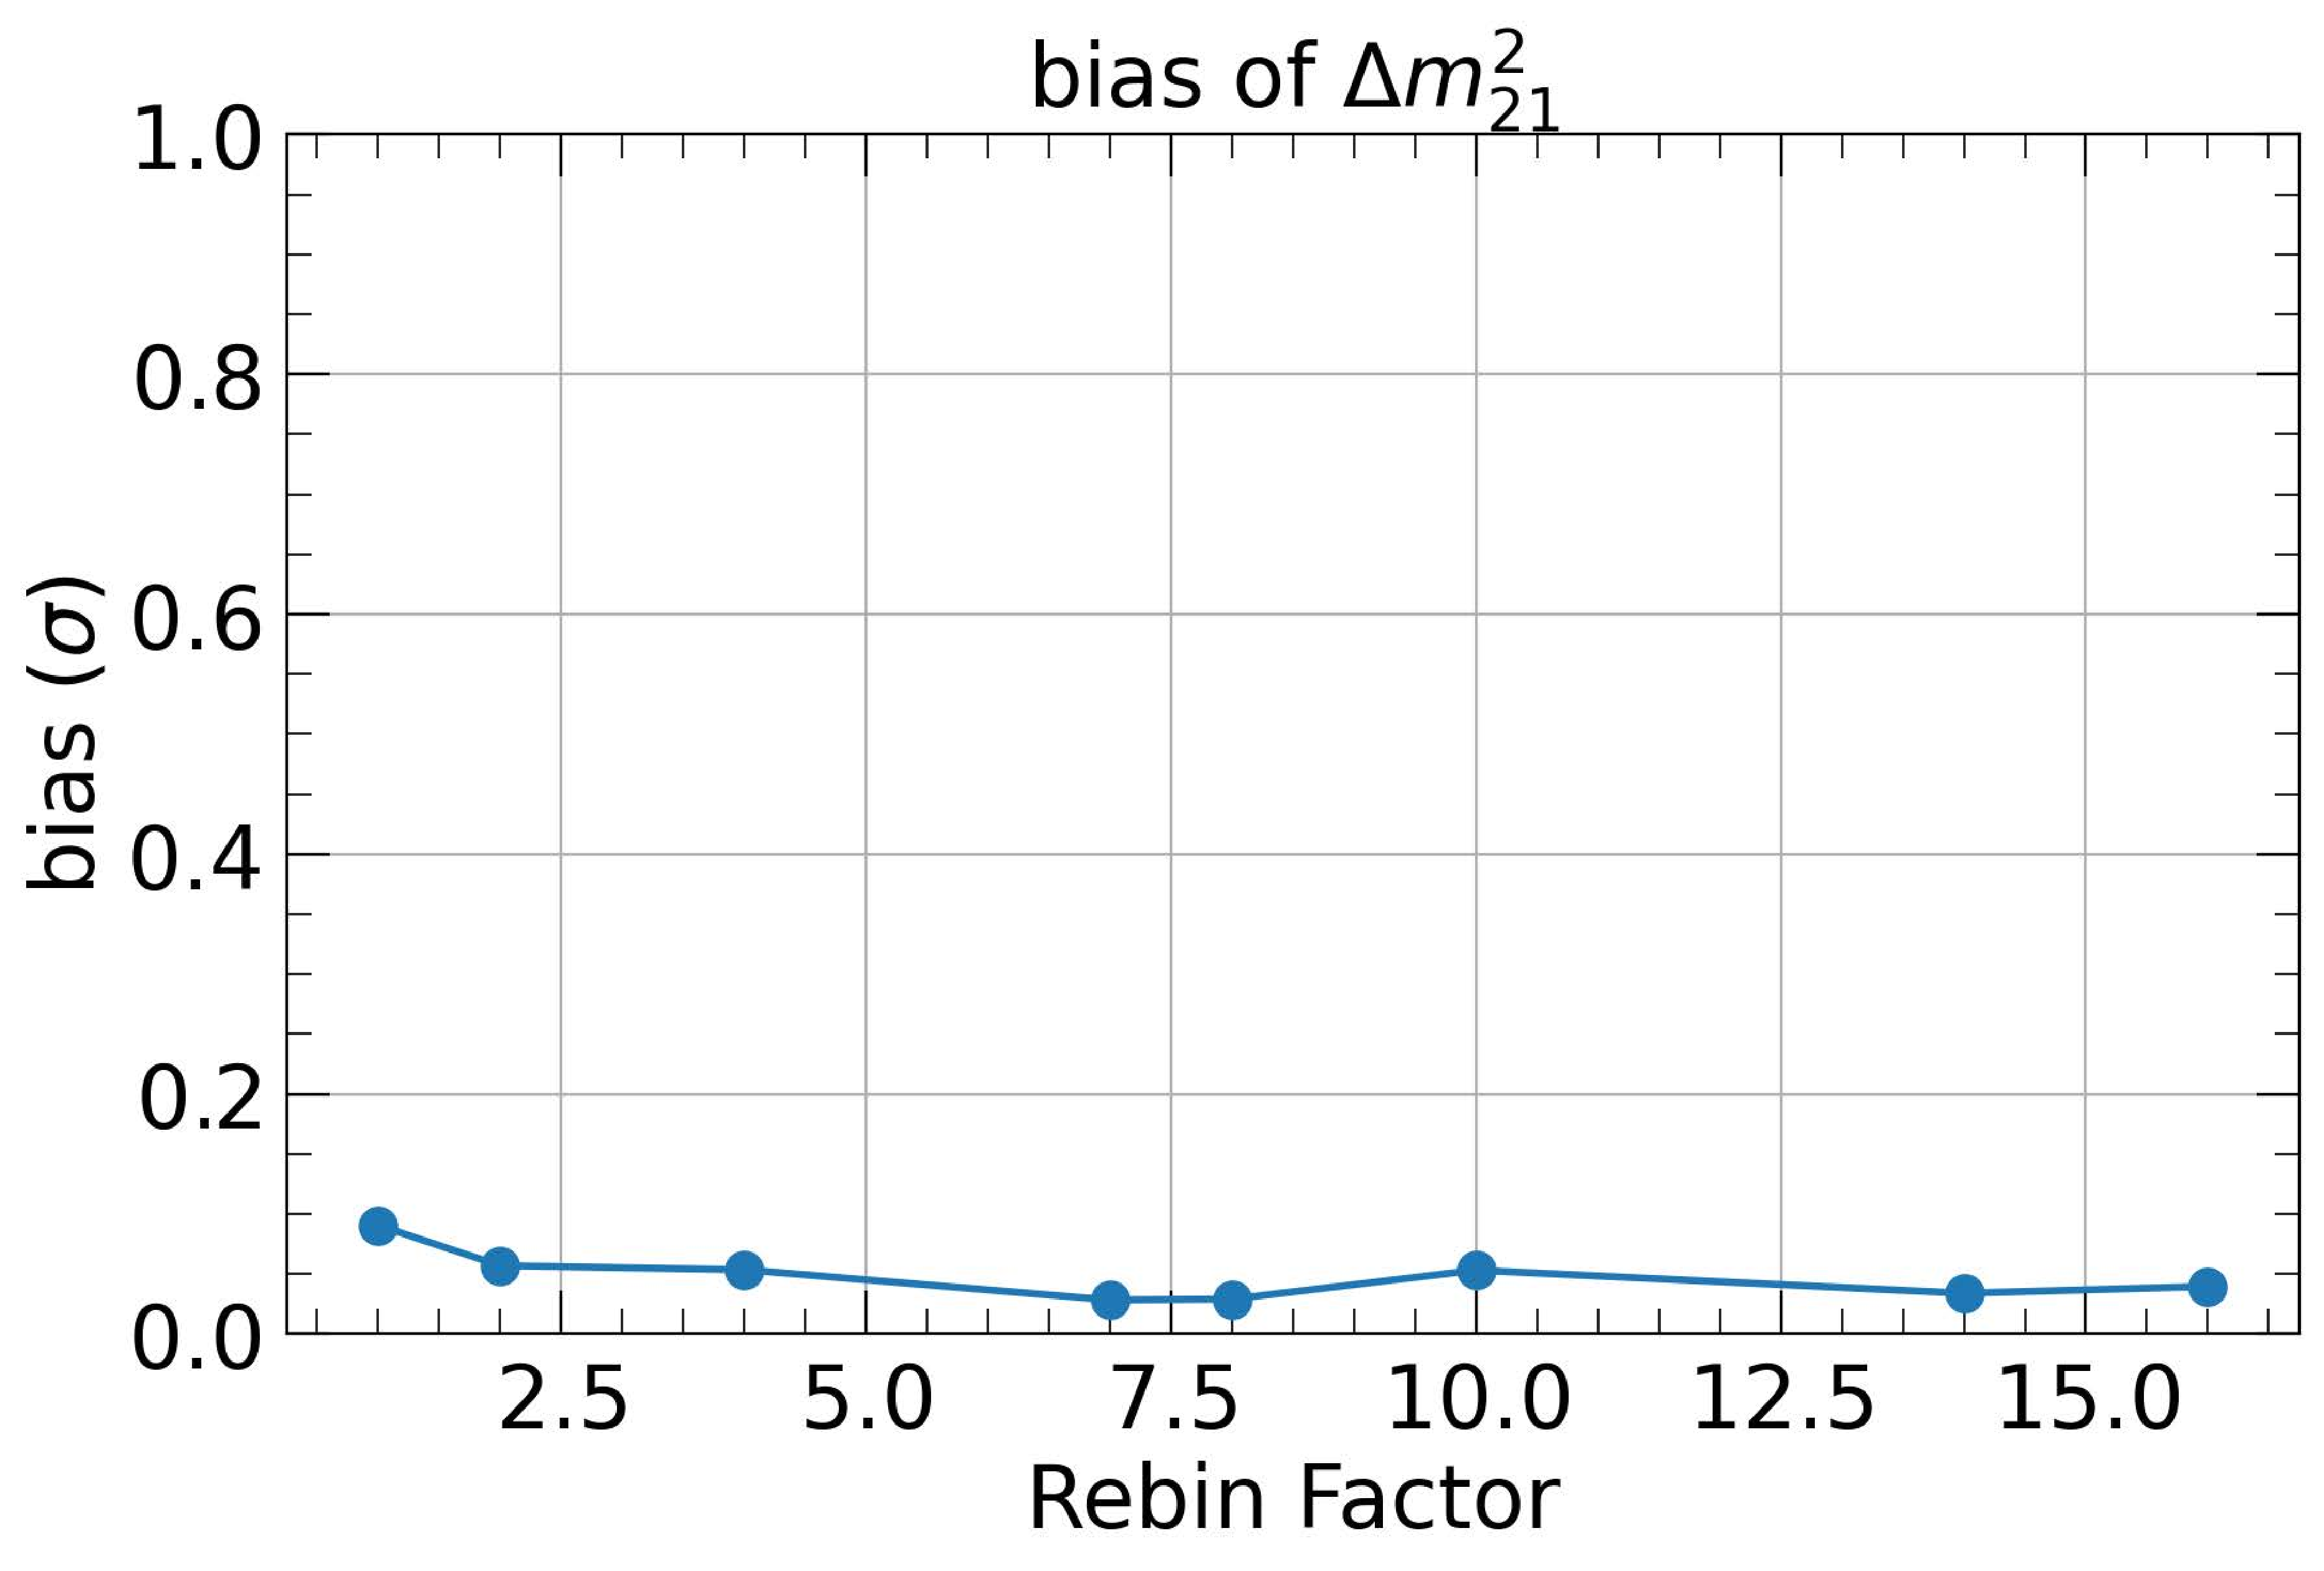
\includegraphics[width=\linewidth]{Img/binning strategy/Jingqin_dmsq21_bias_dif_bins.pdf}
      \caption{$\Delta m^2_{21}$ 偏差随重分 bin 因子的变化。}
      \label{fig:dm2_21_bias_bins}
    \end{subfigure}
    \hfill
    \begin{subfigure}[t]{0.47\textwidth}
      \centering
      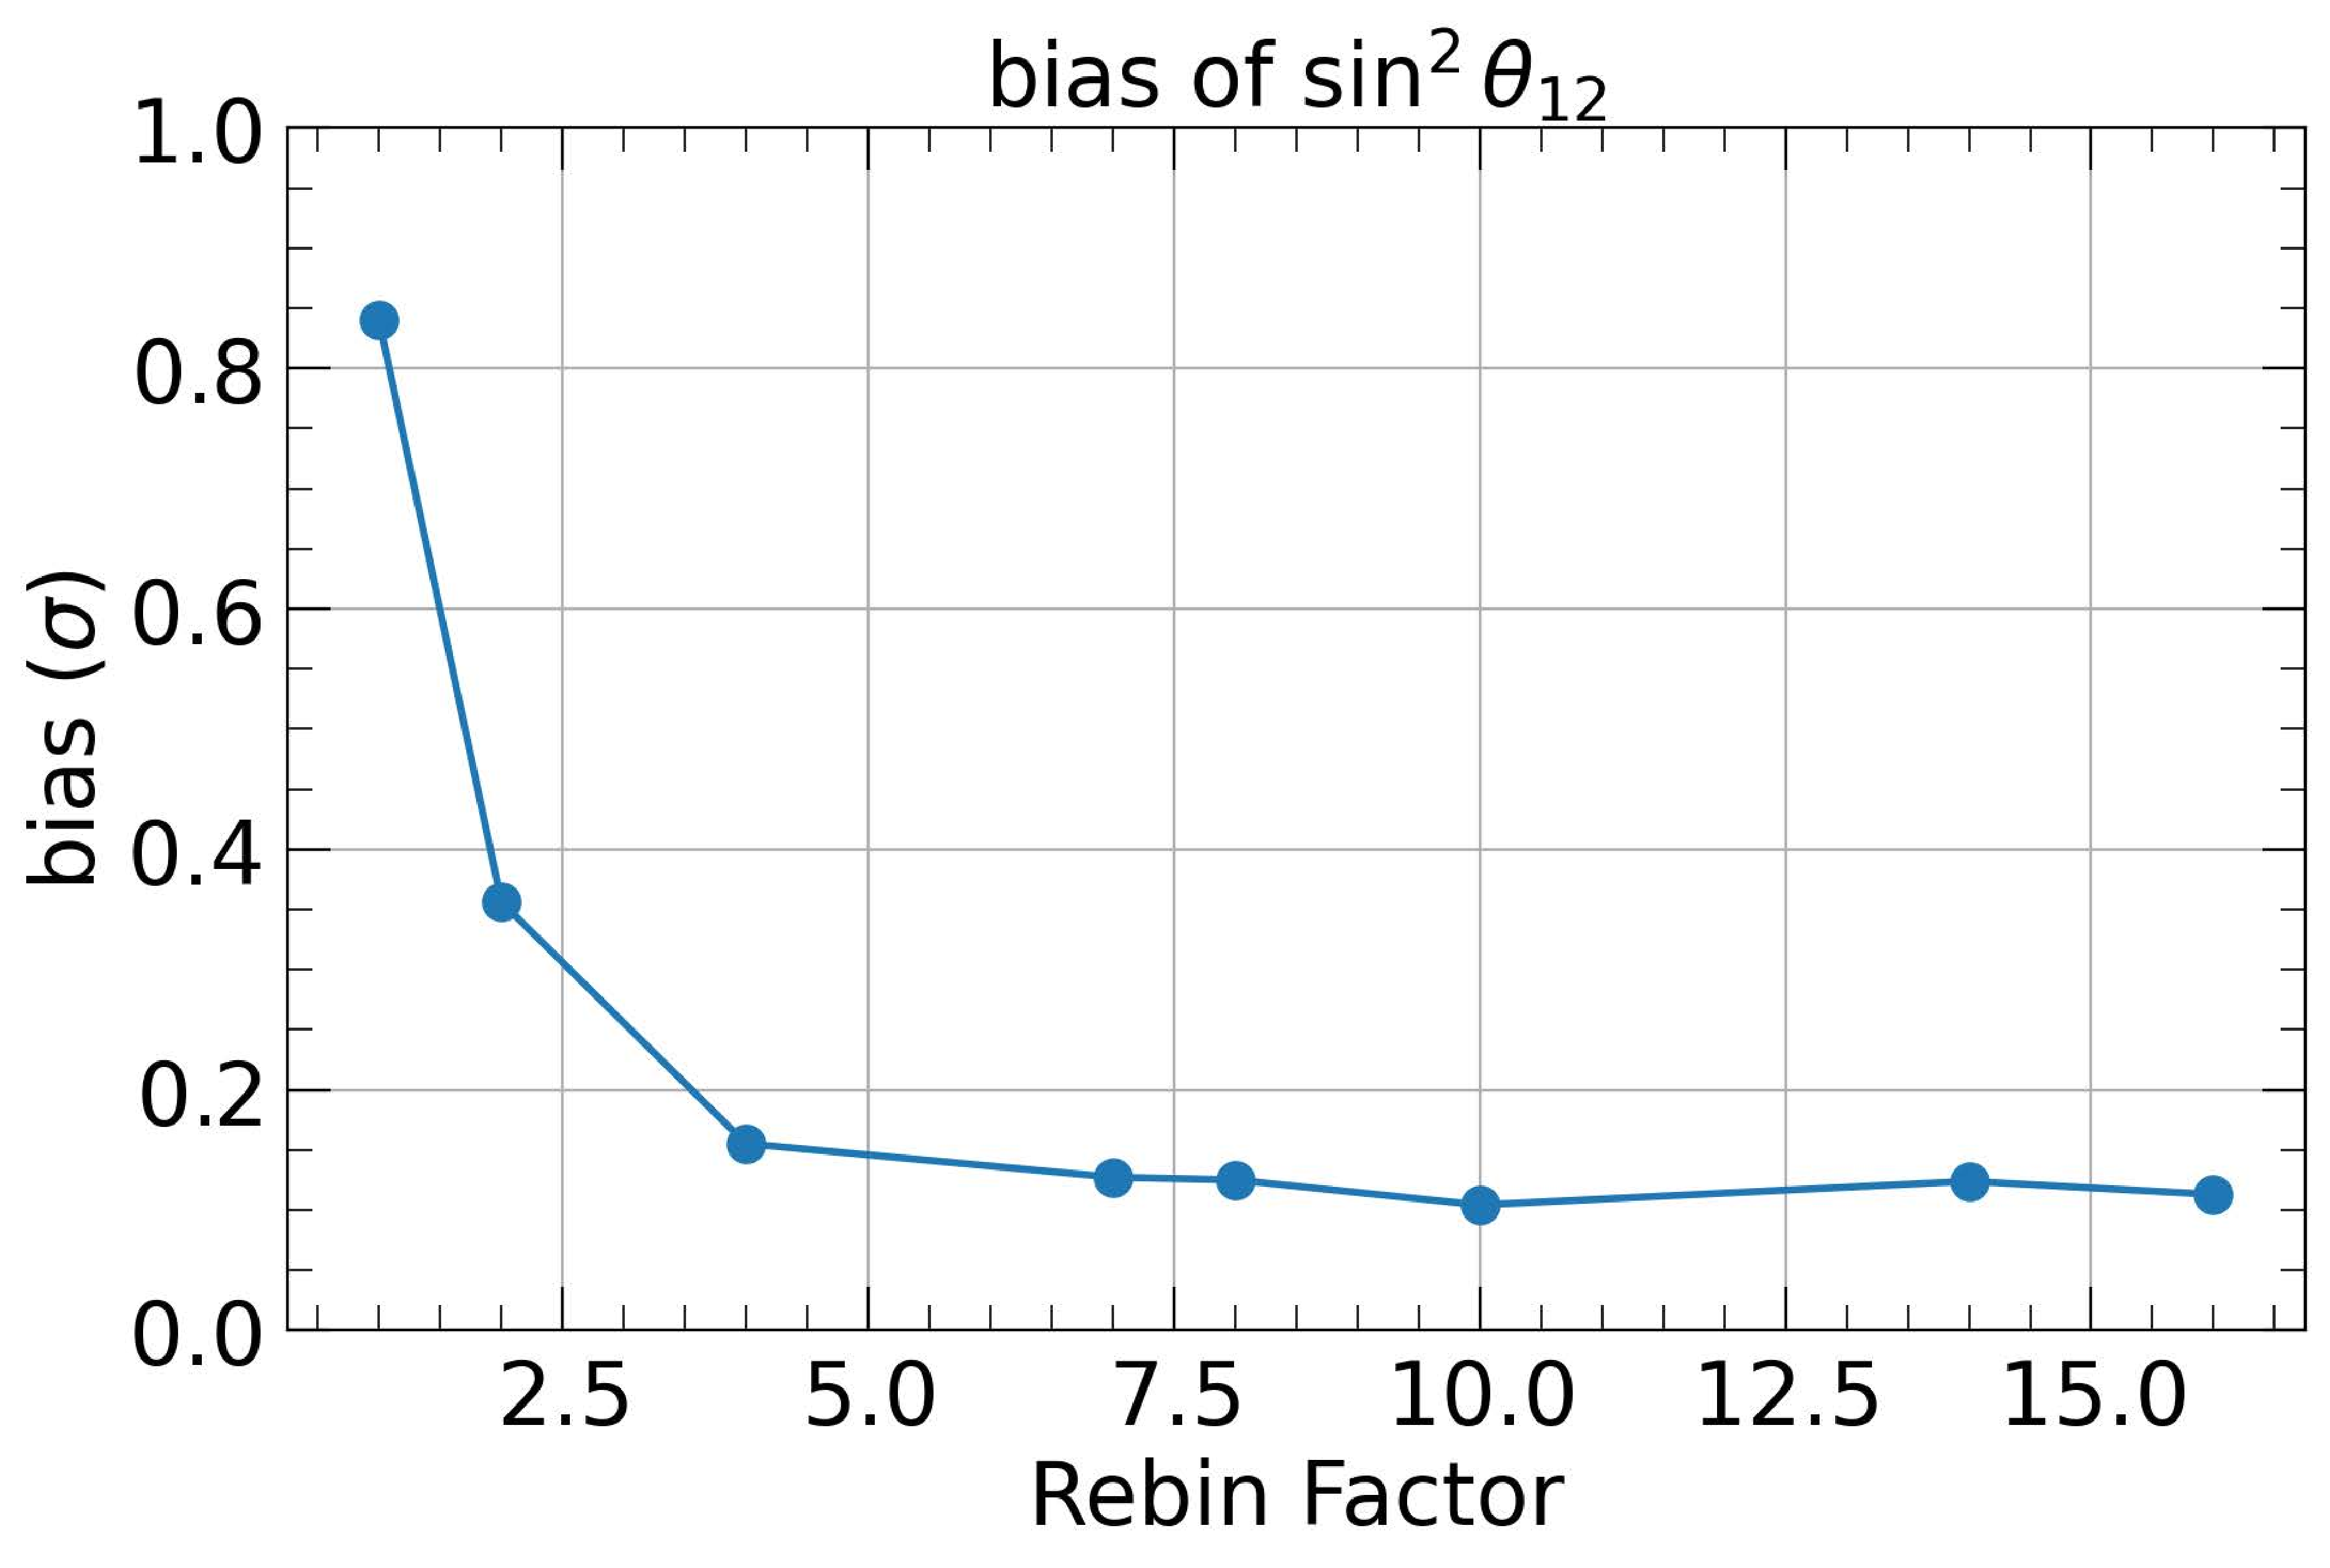
\includegraphics[width=\linewidth]{Img/binning strategy/Jingqin_sinsq12_bias_dif_bins.pdf}
      \caption{$\sin^2\theta_{12}$ 偏差随重分 bin 因子的变化。}
      \label{fig:s12_bias_bins}
    \end{subfigure}
    \bicaption
    {太阳振荡参数偏差随重分 bin 因子的演化。（a）$\Delta m^2_{21}$ 的偏差；（b）$\sin^2\theta_{12}$ 的偏差。}
    {Evolution of the bias of solar oscillation parameters as a function of the rebin factor. Panel (a) shows the bias of $\Delta m^2_{21}$; panel (b) shows the bias of $\sin^2\theta_{12}$.}
    \label{fig:solar_low_stat_bias_bins}
  \end{figure}

\autoref{fig:solar_low_stat_bias_bins} 展示了偏差随重分 bin 因子的变化趋势（以 560 个 bin 为名义配置）。\autoref{fig:dm2_21_bias_bins} 表明，在 30 天曝光下，$\Delta m^2_{21}$ 基本无偏，并且不依赖于重分 bin 因子。另一方面，\autoref{fig:s12_bias_bins} 显示 $\sin^2\theta_{12}$ 对分 bin 策略具有较强依赖性：随着重分 bin 因子增大（bin 数减少），偏差显著下降。从重分 bin 因子 1（560 个 bin，20keV）时约 $0.8\sigma$，降至重分 bin 因子 10（56 个 bin，100keV）时小于 $0.2\sigma$。


\subsection{本节结论}

太阳振荡参数的测量整体上不存在显著挑战。在低曝光条件下，$\Delta m^2_{21}$ 和 $\sin^2\theta_{12}$ 均表现出良好的统计性质。主要结果如下：

\begin{itemize}[leftmargin=*,nosep]
    \item $\Delta m^2_{21}$ 在所有曝光水平下偏差极小（小于 $0.1\sigma$），且不受不同分 bin 选择的影响；
    \item $\sin^2\theta_{12}$ 在极短曝光（30 天）时存在一定偏差，但可通过减少 bin 数（增大 bin 宽至100keV）有效控制；
    \item 在当前研究的名义配置下，JUNO 在首月运行内即可达到优于当前全球结果的测量精度。
\end{itemize}

因此，只要通过适当的探测器刻度和背景建模（尤其是地中微子背景）对系统误差进行良好控制，JUNO 有望在运行最初几个月内实现对太阳振荡参数的世界领先测量。

\section{反应堆中微子能谱分bin策略}

\subsection{早期运行阶段的统计限制与Daya Bay实验约束动机}

在 JUNO 早期运行阶段，反应堆中微子能谱测量面临显著的统计限制。特别是作为近探测器设计的 TAO 子实验，其主要目标是以优异的能量分辨率直接测量反应堆中微子能谱的精细结构。然而在实验启动初期，TAO 尚无法积累足够的统计量以对反应堆谱形进行高精度约束。另一方面，TAO 早期可能无法获得反应堆停堆（reactor-off）数据，这对背景估计的精确性非常重要。这意味着 JUNO 在首篇物理结果中，无法完全依赖自身或 TAO 的数据独立确定反应堆中微子能谱的不确定性。

在缺乏高统计量近点能谱测量的情况下，反应堆中微子模型不确定性将直接传播至远端振荡分析中。由于 JUNO 采用前向折叠（forward-folded）能谱拟合方法，理论反应堆能谱需要经过振荡效应、IBD 截面以及探测器响应函数卷积后，与重建能谱进行比较。因此，输入反应堆能谱的形状误差会以高度相关的方式影响最终振荡参数的提取。如果不加控制，这种模型依赖可能在统计误差尚未完全主导时，就成为系统误差的主要来源。

而Daya Bay 实验已积累了超过 550 万个电子反微中子事件的高统计数据。这些高统计数据可为 JUNO 提供对初始反应堆反中微子能谱的有力约束，从而显著降低远场振荡分析中由谱形不确定性引入的系统误差。

基于上述考虑，JUNO 首篇物理结果计划采用与大亚湾实验（Daya Bay, DYB）的联合分析策略。大亚湾近探测器具有极高统计量的反应堆中微子能谱测量结果，可为反应堆谱形提供外部约束。然而，由于 DYB 探测器能量分辨率相对有限，其对谱形精细结构的约束能力存在固有尺度限制。因此，在将 DYB 数据引入联合拟合框架时，必须对反应堆能谱的自由度进行合理分段，使其既能有效吸收模型不确定性，又不超出 DYB 实验的约束能力。

这一本质上的统计与系统误差之间的张力，构成了反应堆能谱分段（segmentation）策略设计的出发点。下一节将介绍联合分析框架及其数学形式化描述。

\subsection{联合分析框架}

为了在联合拟合中把近场高统计信息形式化地纳入，我们采用对大亚湾数据的 χ² 约束。具体地，我们将大亚湾测得的 prompt 能谱 $\boldsymbol{M}^{\rm DYB}$（经归一化并去除振荡与乏燃料/非平衡修正）与模型预测 $\boldsymbol{T}^{\rm DYB}$ 进行比较，得到如式~(\ref{eq:Chisq:DYB}) 所示的 $\chi^2_{\mathrm{DYB}}$。其中协方差矩阵 $\mathbf{Cov}$ 包含了统计不确定度以及探测、背景和反应堆相关的系统误差分量，模型预测 $\boldsymbol{T}^{\rm DYB}$ 在构造时包含 IBD 截面、液体闪烁体非线性、能量分辨以及 IAV 等探测器效应（均按文献~\cite{PhysRevLett.134.201802} 的响应模型处理）。在联合最小化时，我们将 JUNO 的 χ² 与上述 $\chi^2_{\mathrm{DYB}}$ 相加，再加上来自大亚湾对 $\sin^2\theta_{13}$ 与 $\Delta m^2_{31}$ 的外部高精度先验项，得到总目标函数式~(\ref{eq:Chisq:Total})。

（注：式~(\ref{eq:Chisq:Total}) 中的 $\chi^2_{\rm JUNO}$ 包含 JUNO 观测谱、背景项、探测器响应与其它拉项约束；在实现时我们按段级参数 $\{\alpha_i\}$ 将 DYB 的约束映射到 JUNO 的谱预测中。）

为了利用近点探测器对反应堆能谱的约束，我们将 Daya Bay实验提供的经过去振荡、去 SNF/Non-Eq 修正并按每次裂变归一化的提示能谱 $\boldsymbol{M}^{\rm DYB}$ 纳入联合拟合。Daya Bay 的数据项采用带完整协方差矩阵的 χ²：  
\begin{equation}  
\chi^2_{\rm DYB} = (\boldsymbol{M}^{\rm DYB} - \boldsymbol{T}^{\rm DYB})^\top \mathbf{Cov}^{-1} (\boldsymbol{M}^{\rm DYB} - \boldsymbol{T}^{\rm DYB}),  
\label{eq:Chisq:DYB}  
\end{equation}  
其中 $\boldsymbol{T}^{\rm DYB}$ 为我们用相同反应堆谱模型和 DYB 给定的响应映射（包括 IBD 截面、非线性、分辨率与 IAV 等效应）计算得到的预测谱，$\mathbf{Cov}$ 为 DYB 提供的完整协方差矩阵（包含统计与各类系统误差）。将 DYB 纳入能显著约束反应堆谱的系统不确定性并降低模型相关偏差。

此外，我们还在拟合中引入来自 Daya Bay 等实验对 $\sin^2\theta_{13}$ 与 $\Delta m^2_{31}$ 的外部约束（Gaussian prior），作为额外的拉项。最终的总目标函数为  
\begin{equation}
\begin{aligned}
\chi^2_{\rm Total}
&= \chi^2_{\rm JUNO} + \chi^2_{\rm DYB} \\
&\quad + \left( \frac{\sin^2\theta_{13} - \sin^2\theta_{13}^{\rm DYB}}{\sigma(\sin^2\theta_{13}^{\rm DYB})} \right)^2 \\
&\quad + \left( \frac{\Delta m_{31}^2 - \Delta m_{31}^{2,\rm DYB}}{\sigma(\Delta m_{31}^{2,\rm DYB})} \right)^2 \, .
\end{aligned}
\label{eq:Chisq:Total}
\end{equation}

为降低反应堆谱形不确定性对远场振荡分析的影响，我们采用将 Daya Bay 的高统计近点能谱数据引入 JUNO 拟合的联合分析框架。联合分析的关键思路是对连续的反应堆 $\bar\nu_e$ 能谱进行分段（energy segmentation），并用近点的高统计数据对每一段的归一化自由度施加外部约束，从而在保证灵敏度的同时控制模型依赖性。


具体做法如下：

\begin{enumerate}
  \item \textbf{谱段化（segmentation）}
  
  将初始反应堆能谱 $S(E)$ 在能量空间上划分为若干不重叠的能段 $\{I_i\}$，并把原始连续谱表示为各段基形 $S_i(E)$ 的线性组合：
  $$
    S(E)\;\approx\;\sum_{i}\alpha_i\,S_i(E),\qquad S_i(E)\equiv S(E)\,\mathbf{1}_{E\in I_i},
  $$
  其中 $\alpha_i$ 为第 $i$ 段的归一化因子（拟合参数），$\mathbf{1}_{E\in I_i}$ 为段指示函数。
  
  \item \textbf{段内保持谱形固定、段间自由调节}
  
  在每一能段 $I_i$ 内假定谱形（相对能量依赖）由基底 $S_i(E)$ 给出且保持不变，仅通过整体缩放因子 $\alpha_i$ 来调节该段的强度。不同段之间的相对强度由 $\{\alpha_i\}$ 在拟合过程中独立调整，从而将连续谱的无限维自由度离散化为一组有限维参数问题。
  
\item \textbf{近点数据的外部约束}
  
  作为近点高统计量数据的代表实验，Daya Bay 数据对这些段级归一化因子给予外部约束：在联合拟合中加入一项表征 DYB 与模型偏差的 χ²（或协方差先验），使得 $\{\alpha_i\}$ 在拟合时既能响应远场（JUNO）数据的需求，又受近点高统计数据的牵引与正则化。数学上，联合目标可写为式~(\ref{eq:Chisq:Total})，其中 $\theta$ 表示振荡参数，$\chi^2_{\rm DYB}$ 给出 $\{\alpha_i\}$ 的先验信息或协方差约束（其具体形式见式~(\ref{eq:Chisq:DYB})）。
\end{enumerate}


将连续谱自由度离散化为段间归一化因子，可以显著降低谱形不确定性对振荡参数估计的敏感性；通过引入近点高统计约束，联合拟合能够抑制模型引起的偏差，同时保留远场对振荡结构（例如 $L/E$ 谱振荡）的辨识能力；段宽（segment size）为关键自由量：若段宽过小，会超出近点探测器（DYB）在能量分辨与统计上的约束能力，导致拟合出现非物理波动或过拟合；若段宽过大，则反应堆模型依赖性增强，无法反映局部谱形差异。故段宽的选择必须在“模型相关系统误差”与“统计不确定性／约束能力”之间取得平衡。
        
综上所述，本节采用的分段联合拟合策略实质上是用 Daya Bay 的高统计近点信息“锚定”反应堆谱的局部形状（local shape），从而为 JUNO 的远场振荡分析提供稳健且可控的谱形先验。后续小节将给出具体的段划方案、Toy-MC 验证设计与最终的段宽选择依据。
    
\subsection{半模型独立方法}

反应堆能谱是占主导地位的系统误差来源。我们采用一种半模型独立的策略：利用Daya Bay 的高统计数据约束基准谱形，而理论上的 Huber–Müller（HM）预测仅用于 JUNO 特有的修正项（例如不同堆芯间的裂变份额差异、乏核燃料与非平衡校正等）。
为在尽量减少理论模型依赖的前提下，充分利用近点高统计数据对反应堆谱形的约束，我们采用一种半模型独立（semi-model-independent）的谱预测与拟合框架。对第 $r$ 号反应堆，入射中微子谱记为

\begin{equation}\begin{aligned}
\phi'_r(E_\nu)
&=T_{\rm live}\,
\frac{P_r}{\sum_{r,i} f_{r,i}\,\varepsilon_{r,i}}
\Bigg[
S_{\rm model}(E_\nu)
+\sum_i f_{r,i}\,S_i^{\rm HM}(E_\nu)
\Bigg] \\
&\quad
+ T_{\rm live}\,\phi^{\rm SNF}_r(E_\nu)
+ T_{\rm live}\,\phi^{\rm NonEq}_r(E_\nu)
+ \sum_i \Delta f_{r,i}\,S_i^{\rm HM\text{-}Bump}(E_\nu)\, .
\end{aligned}
\label{eq:phi:semi-model-independent}
\end{equation}

下面逐项解释该表达式的物理意义、实现方法与半模型独立实现细节。

\paragraph*{（1）归一化因子与探测器活跃时间}
前置因子 $T_{\rm live}\frac{P_r}{\sum_{r,i} f_{r,i}\,\varepsilon_{r,i}}$ 为总体归一化／标度项：$P_r$ 为第 $r$ 号堆的热功率，$\varepsilon_{r,i}$ 为探测器对应同位素 $i$ 的裂变能量，$T_{\rm live}$ 为活跃取数时间。该部分仅决定总事件率尺度，与谱形的“局部形状”是分离的，便于在拟合中将幅值与形状分别处理。

\paragraph*{（2）模型无关的主项 $S_{\rm model}(E_\nu)$}
$S_{\rm model}$ 表示一套“通用基底”或主谱形模板，既可以取名义的 Huber--Müller（HM）模型、summation 模型，也可以用“经验段化（segment）基底”直接构造。在半模型独立（semi-model-independent）框架中，关键点不是把 $S_{\rm model}$ 当作“绝对真实值”，而是将其作为起始形状／段内模板：通常把能量区间划分为若干段（segments），段内的相对谱形由 $S_{\rm model}$ 给出（即段内刚性），但每段的整体归一化作为自由参数（或带 DYB 先验的 nuisance）在拟合中允许独立浮动，即“段内刚性、段间自由”，从而实现对模型的弱依赖而非完全倚赖。

\paragraph*{（3）非平衡修正项 $\phi^{\rm NonEq}_r(E_\nu)$}
对应项为 $T_{\rm live}\,\phi^{\rm NonEq}_r(E_\nu)$。该项表示由于长寿命裂变产物尚未达到稳态所引起的非平衡修正。在本分析中，该贡献被整体作为一个小的能量相关通量修正项处理，而不再在同位素层面展开，其不确定度通过独立协方差矩阵传播。

\paragraph*{（4）乏燃料贡献 $\phi^{\rm SNF}_r(E_\nu)$}
对应项为 $T_{\rm live}\,\phi^{\rm SNF}_r(E_\nu)$。该项表示堆外乏燃料池中残余 $\beta$ 衰变所产生的反中微子贡献。由于其强度相对主反应堆裂变通量较小，且谱形可通过堆厂运行记录估算，因此作为一个独立的附加通量项处理。

\paragraph*{（5）补偿／差分项 $\sum_i \Delta f_{r,i}\,S_i^{\rm HM\text{-}Bump}$（关键项）}
令 $\Delta f_{r,i}\equiv f_{r,i}^{\rm JUNO}-f_i^{\rm DYB}$ 表示 JUNO（或某个堆）与 DYB 参考之间的裂变份额差异。补偿项把同位素级别的“已知／观测到的大尺度谱形偏差”（例如 HM-bump）作为基函数 $S_i^{\rm HM\text{-}Bump}$ 投影，并用 $\Delta f_{r,i}$ 线性组合来修正。该设计的物理动机是：当利用 DYB 的高统计谱去“锚定”整体谱形时，JUNO 与 DYB 在燃料构成上不可避免有差别，差别会引起可预测的谱形偏移；把这部分显式写成线性补偿项，使得联合拟合时 DYB 所能很好约束的“共同成分”与 JUNO 特有的“堆芯差分成分”被明确区分，从而减少把堆芯差异误认作振荡信号的风险。

从式~(\ref{eq:phi:semi-model-independent})的分解可以直接看出分段选择为何会引发上述的二择一问题。式中共有几类贡献：

\begin{itemize}
\item 一个由 $S_{\rm model}(E_\nu)$ 与若干反应堆中微子能谱基底（segments）所表示的“主项”，它提供了段内相对谱形的模板与段间的归一化自由度，其中段内谱形是刚性的，依赖于模型；
\item 一组同位素／模型相关的结构项（如使用 HM-Bump 模型的差分投影
  $\sum_i \Delta f_{r,i}\,S_i^{\rm HM\text{-}Bump}$），这一部分是模型相关的；
\item 若干次要的整体通量修正项（$\phi^{\rm NonEq}$、$\phi^{\rm SNF}$ 等），这部分也部分依赖于模型。
\end{itemize}
    

因此，分段策略等价于在模型空间中引入了一组附加自由度（段系数），这些自由度用于在拟合中调整 $S_{\rm model}$ 的局部归一化以匹配数据。问题的关键在于：数据（主要由 Daya-Bay 等近点实验提供的约束）对这些自由度的约束能力是有限的。若我们把能量区间分成 $N_{\rm seg}$ 段，则会新增约 $N_{\rm seg}$ 个段系数自由度；这些自由度必须由近点数据通过协方差或 likelihood 条款来约束，否则拟合会出现不受控的局部波动，从而导致模型依赖性增强，系统误差增大。因此核心矛盾是系统误差与统计误差的平衡。

\paragraph*{核心矛盾（物理与统计的折中）}
在采用“段化（segment）”策略用近点高统计数据约束反应堆谱时存在根本性的二择一：

\begin{itemize}
\item \textbf{分段过多（段宽太细）}
\begin{itemize}
\item \textbf{问题：}当段宽小于近点探测器（如 Daya Bay）的有效能量分辨尺度时，近点数据无法对每一段提供独立而可靠的约束，统计误差增大；拟合会出现未被约束的高频自由度，导致在重建谱中呈现振荡型或非物理性的结构（over-fitting / unphysical wiggles）。
\item \textbf{后果：}拟合过程可能用段系数“吸收”真实的振荡微结构（例如由 $\Delta m^2_{31}$ 引起的小尺度波动），从而弱化对振荡参数的灵敏度或引入偏差。
\end{itemize}
\item \textbf{分段过少（段宽太宽）}
\begin{itemize}
\item \textbf{问题：}段间自由度被过度限制，段内谱形假定刚性——若真实谱存在局部结构或堆芯间差异，这些将无法被段化自由度吸纳，只能依赖理论模型来修正。
\item \textbf{后果：}对理论谱模型的依赖增强，模型相关系统误差（model-dependent bias）被放大，使振荡参数测量的系统容差变差且难以量化。
\end{itemize}
\end{itemize}

因此，段宽选择本质上是在“模型相关系统误差”和“统计不确定性／约束能力”之间寻找平衡。

\subsection{Toy-MC 研究}

为量化上述折中并给出可操作的分段（段宽）选择准则，我们设计一组 Toy-MC 实验，用相同的拟合框架进行拟合，比较两种代表性情况下振荡参数的精度：

\begin{itemize}
\item \textbf{固定反应堆模型情形（Fixed model）：}使用单一名义谱（例如 Huber--Müller 模型或 summation 模型）生成伪数据。该情形评估统计波动与方法本身的行为。
\item \textbf{变化反应堆模型情形（Model-variation）：}基于最新的核数据库构建一组带有精细结构的反应堆能谱，在生成伪数据时对反应堆谱引入物理上合理的扰动（例如随机化的分支比和同位素产额），然后使用名义模板拟合。该情形评估“模型依赖”对振荡参数的影响。
\end{itemize}

\textbf{目标：}对一系列候选段宽（segment widths）比较两类情形下对关键振荡参数的精度（precision），并据此挑选使模型依赖引入的额外系统误差最小的段宽。

\paragraph*{Toy-MC 实验设计}
反应堆中微子能谱范围为 $1.8$--$13\,\mathrm{MeV}$，在该能区范围内选取不同的分 bin 策略。对于每个分段策略，生成 5000 个伪实验数据集。

\begin{figure}[htbp]
\centering
\begin{subfigure}[t]{0.45\textwidth}
\centering
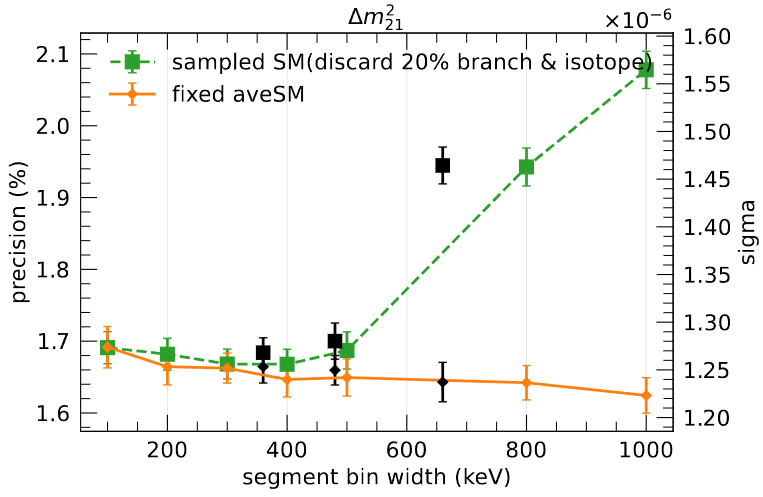
\includegraphics[width=\linewidth]{../groupA_technote/5_oscillation/segment_dmsq21.png}
\caption{}
\label{fig:segment_dmsq21}
\end{subfigure}
\hfill
\begin{subfigure}[t]{0.45\textwidth}
\centering
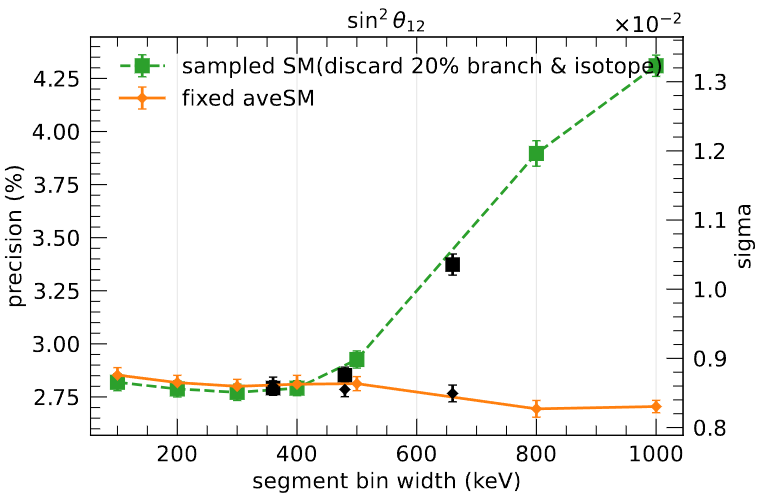
\includegraphics[width=\linewidth]{../groupA_technote/5_oscillation/segment_sinsq12.png}
\caption{}
\label{fig:segment_sinsq12}
\end{subfigure}
\bicaption[段宽对振荡参数精度的影响]{(a) $\Delta m^2_{21}$ 与 (b) $\sin^2\theta_{12}$ 的测量精度随反应堆谱段宽的变化关系。绿色标记／曲线表示在对 Summation 模型进行扰动（随机丢弃 20\% 的裂变分支／同位素）时得到的结果；橙色标记／曲线为固定平均 Summation 模型下的基线精度。黑色点对应以探测器能量分辨为驱动的分段（energy-resolution-driven segmentation），彩色曲线点对应对反应堆谱做的均匀分段。误差线表示由重复 toy/fits 给出的统计不确定度。在约 $300\,\mathrm{keV}$ 附近，额外的模型相关系统不确定度达到最小，表明在模型灵活性与可用统计约束之间达到了较优折中。}{Precision of (a) $\Delta m^2_{21}$ and (b) $\sin^2\theta_{12}$ as a function of reactor-spectrum segment width. Green markers/lines show results when the Summation Model is perturbed (randomly discarding 20\% of branches/isotopes); orange markers/lines indicate the baseline precision with a fixed average Summation Model. Black points correspond to segmentation defined by the detector energy resolution (energy-resolution-driven segmentation), while the colored-line points correspond to uniform segmentation of the reactor spectrum. Error bars denote the statistical uncertainty from repeated toys/fits. The additional model-dependent systematic uncertainty is minimized at a segment width of approximately $300\,\mathrm{keV}$, indicating an optimal trade-off between model flexibility and available statistical constraint.}
\label{fig:segment_comparison}
\end{figure}

图~\ref{fig:segment_comparison} 显示：在约 $300\,\mathrm{keV}$ 的段宽处，模型相关的额外系统不确定度最小——此时绿色曲线与橙色曲线之间的差异最小，说明对模型扰动的抑制效果最好。相反，分段过细会削弱大亚湾（DYB）对每一段的统计约束，增加统计噪声或段间相关性，从而可能导致过拟合；而分段过粗则无法吸收局部谱形差异，使得模型相关系统误差增大。在此处采用的扰动假设下，约 $300\,\mathrm{keV}$ 的段宽在减少模型相关偏差和保持充分统计约束之间提供了一个较优的折中，此时对于$\Delta m_{31}^2$以及$sin^2\theta_{12}$，模型依赖引入的系统误差小于0.3\%。


\subsection{本章小结}

本章围绕能谱分 bin 与分段策略对振荡参数测量的影响进行了系统研究，主要包括两个方面的内容：一是 JUNO 重建能谱的分 bin 策略，二是反应堆中微子本征能谱的分段（segment）策略。

在重建能谱分 bin 策略方面，本章重点研究了不同曝光条件下分 bin 选择对太阳振荡参数测量的影响。研究结果表明，$\Delta m^2_{21}$ 在所有测试曝光水平下均表现出极好的统计稳定性，其拟合偏差始终小于 $0.1\sigma$，且对不同分 bin 方案不敏感，显示出较强的鲁棒性。相比之下，$\sin^2\theta_{12}$ 在极低曝光（如 30 天）情形下会出现一定程度的统计偏差，这主要源于单个 bin 统计量不足时高斯近似的有效性下降。然而，通过适当减少 bin 数、将重建能谱 bin 宽增大至约 $100\,\mathrm{keV}$，可以有效抑制该偏差，使结果恢复稳定。在当前采用的配置和系统控制假设下，JUNO 在首月运行数据中即可达到优于当前全球结果的太阳振荡参数测量精度。因此，JUNO 有望在运行初期实现对太阳振荡参数的世界领先测量。

在反应堆中微子能谱分段策略方面，本章通过大量 Toy-MC 模拟，比较了固定反应堆模型与包含精细结构扰动的变化模型两种情形，在不同 segment 宽度下振荡参数精度与偏差的表现。研究表明，segment 宽度的选择本质上是在模型灵活性与统计约束能力之间寻找平衡：若分段过细，将削弱近点实验对各段自由度的约束能力，增加统计涨落与段间相关性，甚至可能导致过拟合；若分段过粗，则无法吸收局部谱形差异，使模型依赖的系统误差增大。在本文所采用的扰动假设下，当 segment 宽度约为 $300\,\mathrm{keV}$ 时，由模型依赖引入的额外系统不确定度达到最小（小于 $0.3\%$），表明该取值在抑制模型相关偏差与保持充分统计约束之间实现了较优折中。

值得指出的是，本章提出并验证的重建能谱分 bin 策略与反应堆能谱分段方案，已被应用于 JUNO 合作组首篇物理结果的分析工作之中，为相关统计处理方法与系统误差控制提供了定量依据。总体而言，本章工作为 JUNO 在早期运行阶段开展精确振荡参数测量提供了重要的方法学基础，并为后续数据累积阶段的分析优化奠定了可靠框架。


%=====================================================================
%=====================================================================
\chapter{Feldman--Cousins 方法详述}
%=====================================================================

JUNO 实验在低统计量条件下测量 $\Delta m^2_{31}$ 时，常出现轮廓 $\chi^2$ 曲线上的多个局部极小值。这些局域极小值（``bad minima''）会导致按照点估计法构建的置信区间出现多个不连续区间。然而，Asimov 数据集假设观测值等于理论预期值，因而无法体现统计涨落所产生的这些多重极小值现象。因此，为了真实地研究统计波动对置信区间结构的影响，必须借助大量包含随机波动的 Toy Monte Carlo 伪实验进行分析。

\section{Asimov 灵敏度的局限性}

在研究低统计量下拟合与置信区间构造的行为时，需要注意 Asimov 数据集的局限性。Asimov 数据集只反映了理想条件下，无统计偏差下的期望结果，不包含实际观测中的统计扰动。因此，基于 Asimov 的灵敏度评估只给出了理论上的置信区间估计，并未涵盖统计涨落导致的分布非高斯性和偏离情形。其常常给出光滑且单峰的 $\Delta \chi^2$ 侧向轮廓化曲线，从而暗示单一连续的置信区间。但真实观测中存在统计涨落和系统误差波动，这些随机效应会显著改变轮廓形状并产生多重局部极小值。特别是当参数估计过程存在不稳定性或对 $\chi^2$ 响应非线性时（例如多峰或参数边界问题），Asimov 预测可能会严重失真，使得实际覆盖率与名义覆盖率不符。

\begin{figure}[htbp]
  \centering
  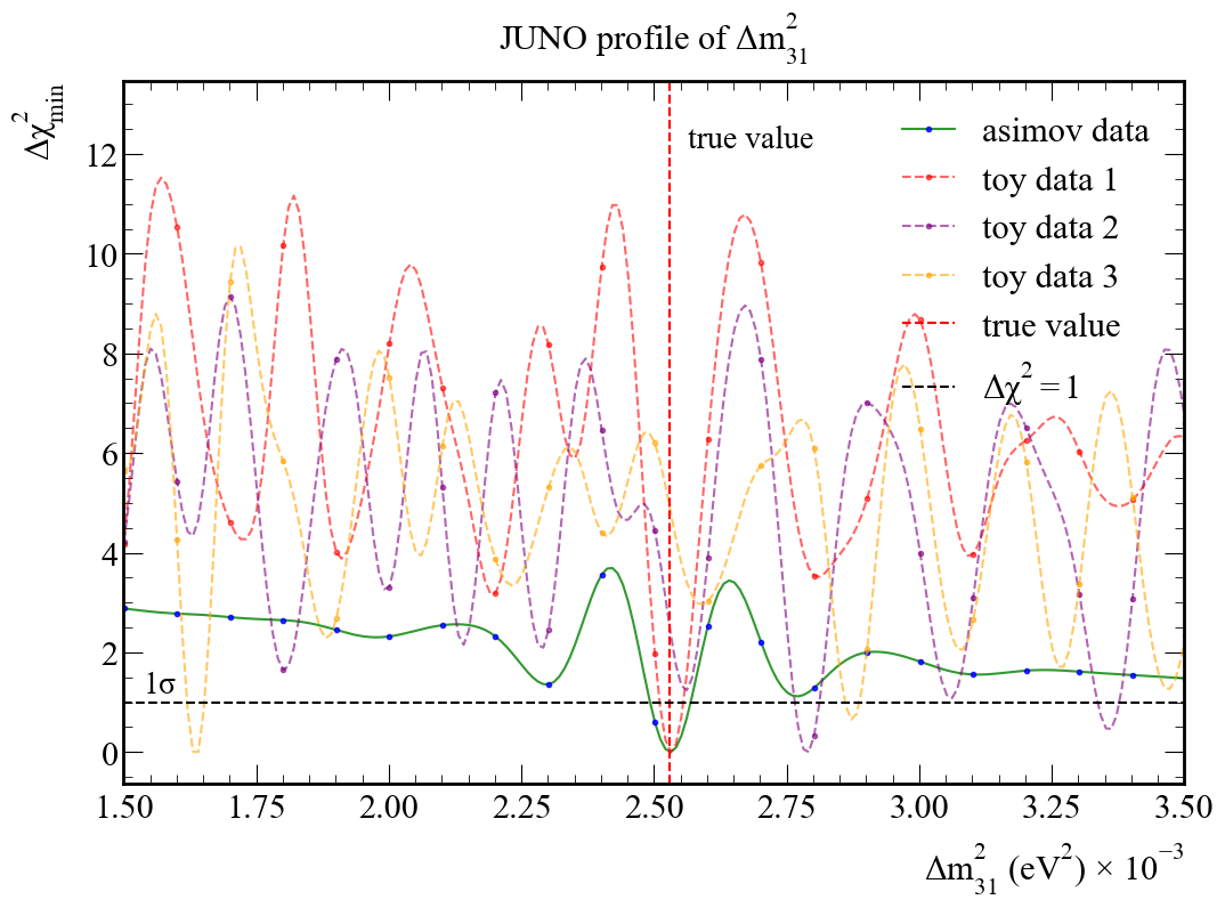
\includegraphics[width=0.9\linewidth]{Img/asimov-data.png}
  \bicaption[$\Delta m^2_{31}$ 的 $\Delta\chi^2$ 轮廓（Asimov 与若干 toy 实验，30 天统计量）]{$\Delta m^2_{31}$ 的 $\Delta\chi^2$ 轮廓（Asimov 与若干 toy 实验，30 天统计量）。绿色实线为 Asimov 数据得到的 $\Delta\chi^2$ 轮廓，显示出靠近真值（红色虚线）处的单一平滑极小值；按 Wilks 近似，这会对应单一连续的 $1\sigma$ 区间（图中黑色虚线为 $\Delta\chi^2 = 1$）。彩色虚线为三个独立 toy-MC 样本的轮廓（包含统计与系统误差波动）。可以看到实际涨落会显著改变轮廓形状：toy 曲线出现许多明显的局部极小值。有些局部极小值比 Asimov 情形更深并且偏离名义真值。这种多峰/多极小值行为会使得使用固定 $\Delta\chi^2$ 截值（Wilks 截断）得到的不一定是连续区间，可能出现不相交的置信域。}{Profile $\Delta\chi^2$ of $\Delta m^2_{31}$ for Asimov and several toy experiments (30 days exposure). The green curve is the Asimov (median) $\Delta\chi^2$ profile, which shows a single, relatively smooth minimum near the true value (red dashed vertical line) and would---under Wilks' approximation---suggest a single continuous $1\sigma$ interval (black dashed horizontal line at $\Delta\chi^2 = 1$). The colored dashed curves are $\Delta\chi^2$ profiles from three independent toy Monte-Carlo realizations (statistical and systematics fluctuations included). Real-data fluctuations substantially distort the profile: toy profiles exhibit many pronounced local minima, some of which are much deeper than nearby Asimov values and lie away from the nominal true value. Such behaviour can produce multiple disjoint confidence regions when one uses fixed $\Delta\chi^2$ thresholds (Wilks cuts).}
  \label{fig:asimov_dm31_profile}
\end{figure}

图~\ref{fig:asimov_dm31_profile} 给出了 30 天统计量下 $\Delta m^2_{31}$ 的实例：绿色曲线是 Asimov 轮廓，呈现单一平滑极小值；而多条彩色虚线（不同 toy-MC 实现）则展现出许多更深或位置不同的局部极小值。实际涨落常使某些局部极小值变得更低且更靠近数据所偏向的值，结果在应用固定 $\Delta\chi^2$ 截断（例如 $\Delta\chi^2 = 1$ 的 1$\sigma$ 判据）时可能得到多个不相交的置信区间或错误的覆盖概率。综上所述，Asimov-based 的灵敏度估计在低统计、参数空间非线性或存在多重解的情形下容易误导决策；因此必须通过大量 toy-MC 生成检验统计量的经验分布（例如采用 Feldman–Cousins 方法）来确定参数相关的临界 $\Delta\chi^2$，从而保证置信区间的频率学覆盖性质。

\begin{figure}[htbp]
  \centering
  \begin{subfigure}[t]{0.48\textwidth}
    \centering
    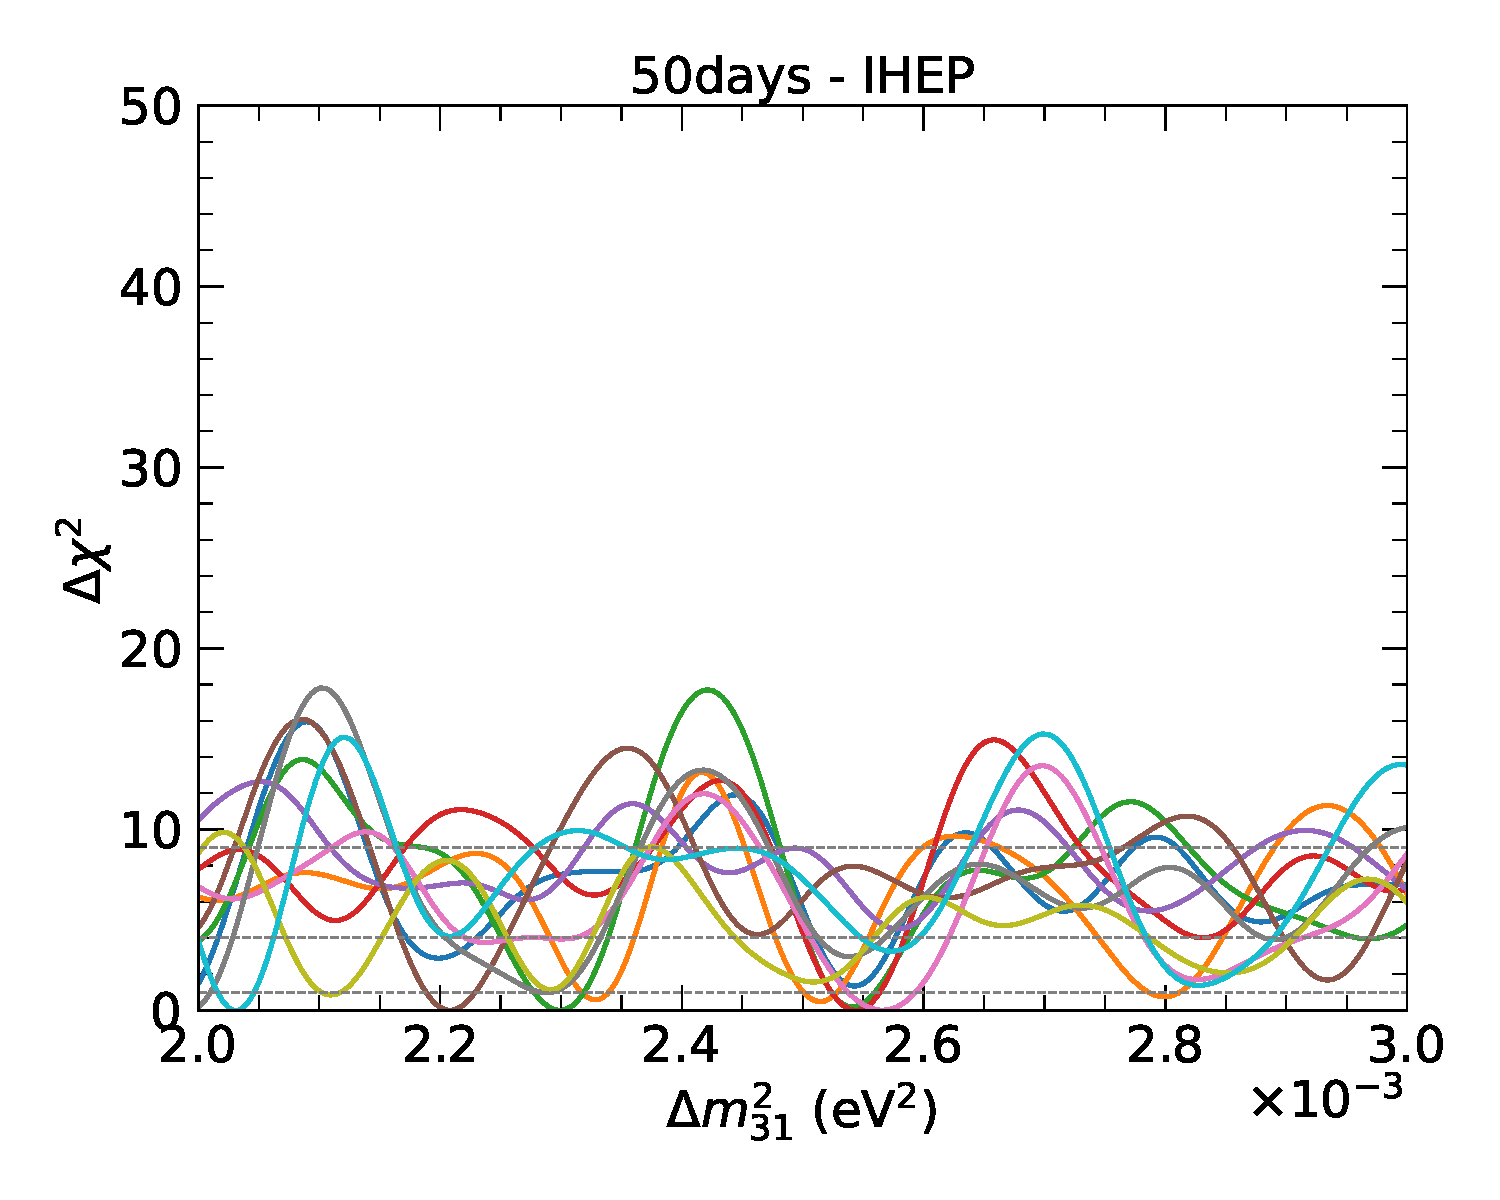
\includegraphics[width=\linewidth]{Img/Jingqin_50days_dmsq31_profile.pdf}
    \caption{50 天统计量}
    \label{fig:dm31_profile_50days}
  \end{subfigure}
  \hfill
  \begin{subfigure}[t]{0.48\textwidth}
    \centering
    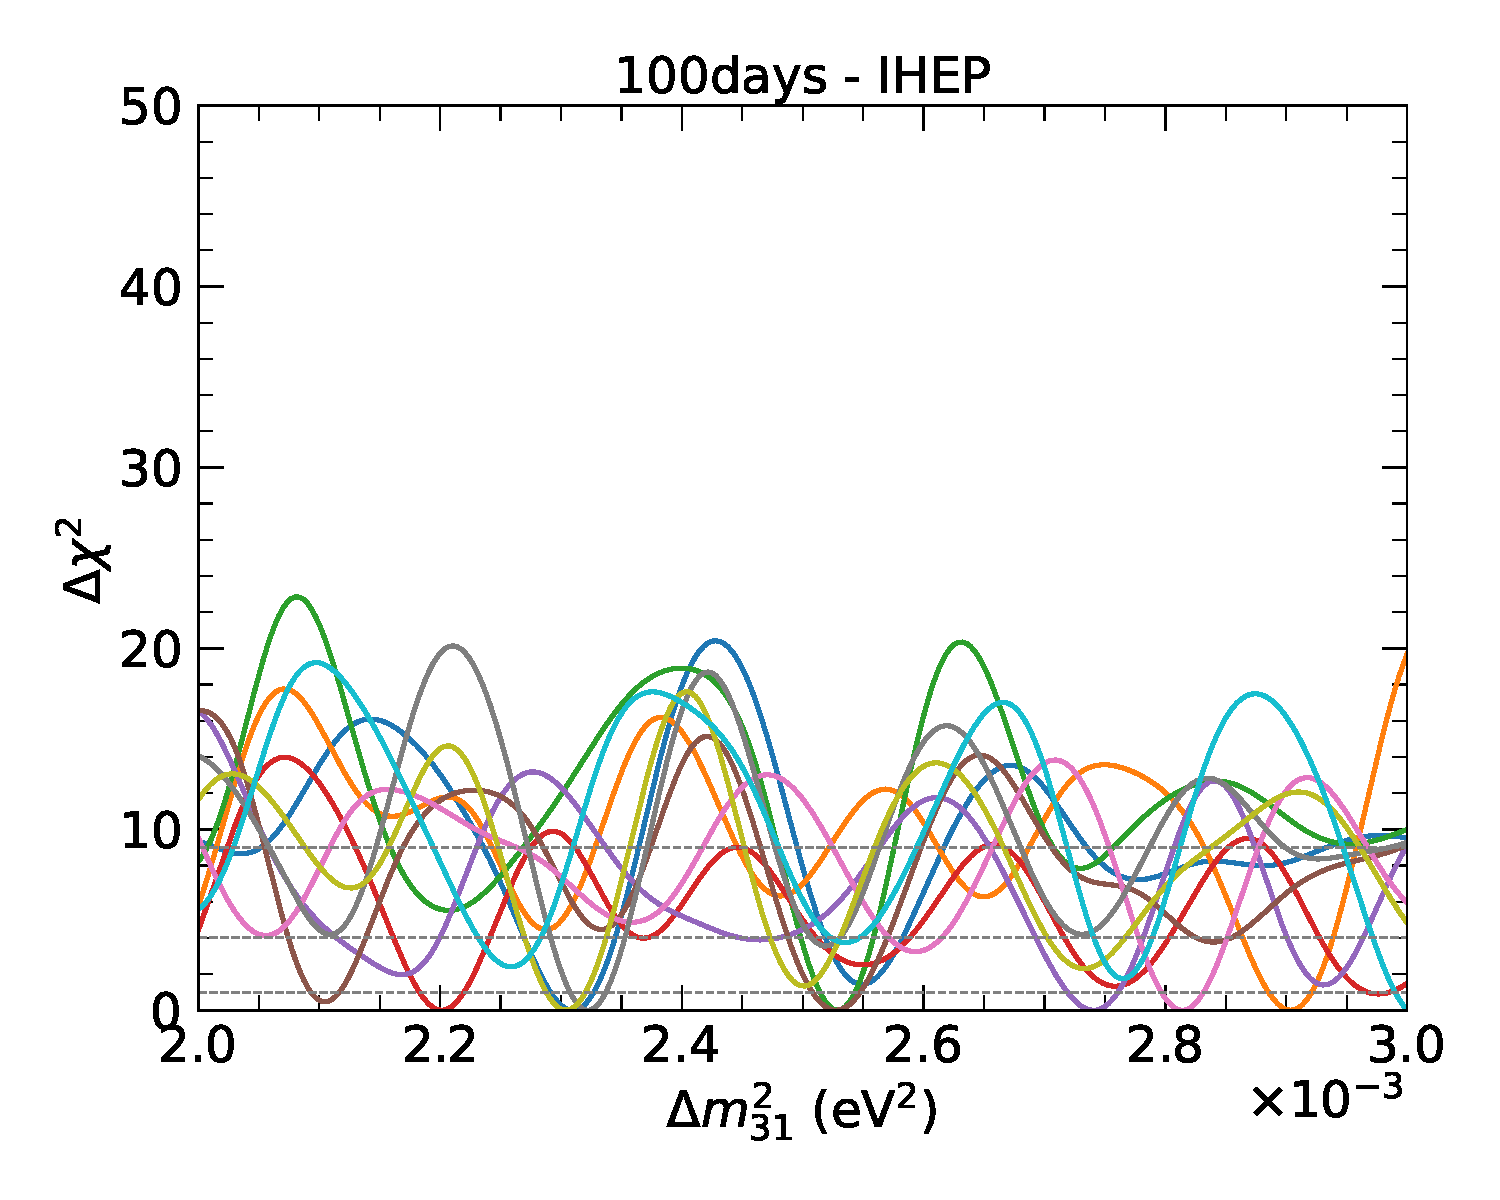
\includegraphics[width=\linewidth]{Img/Jingqin_100days_dmsq31_profile.pdf}
    \caption{100 天统计量}
    \label{fig:dm31_profile_100days}
  \end{subfigure}

  \vspace{0.4em}

  \begin{subfigure}[t]{0.48\textwidth}
    \centering
    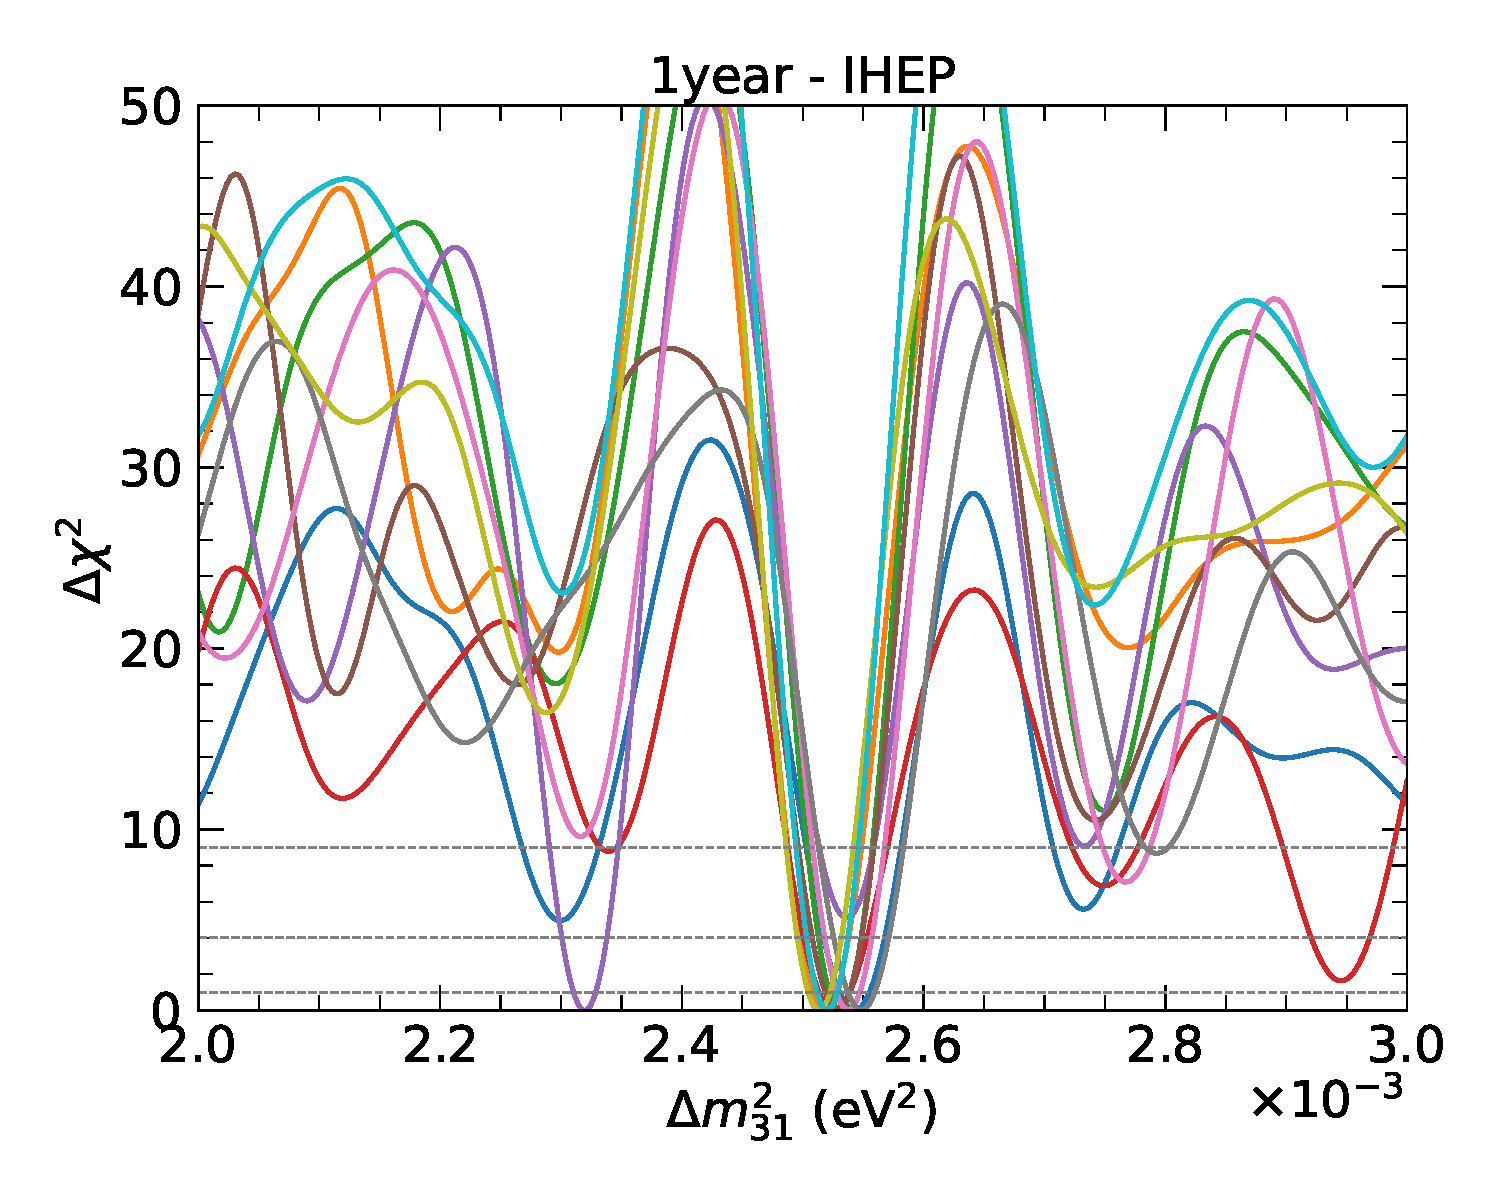
\includegraphics[width=\linewidth]{Img/Jingqin_1years_dmsq31_profile.pdf}
    \caption{1 年统计量}
    \label{fig:dm31_profile_1year}
  \end{subfigure}
  \hfill
  \begin{subfigure}[t]{0.48\textwidth}
    \centering
    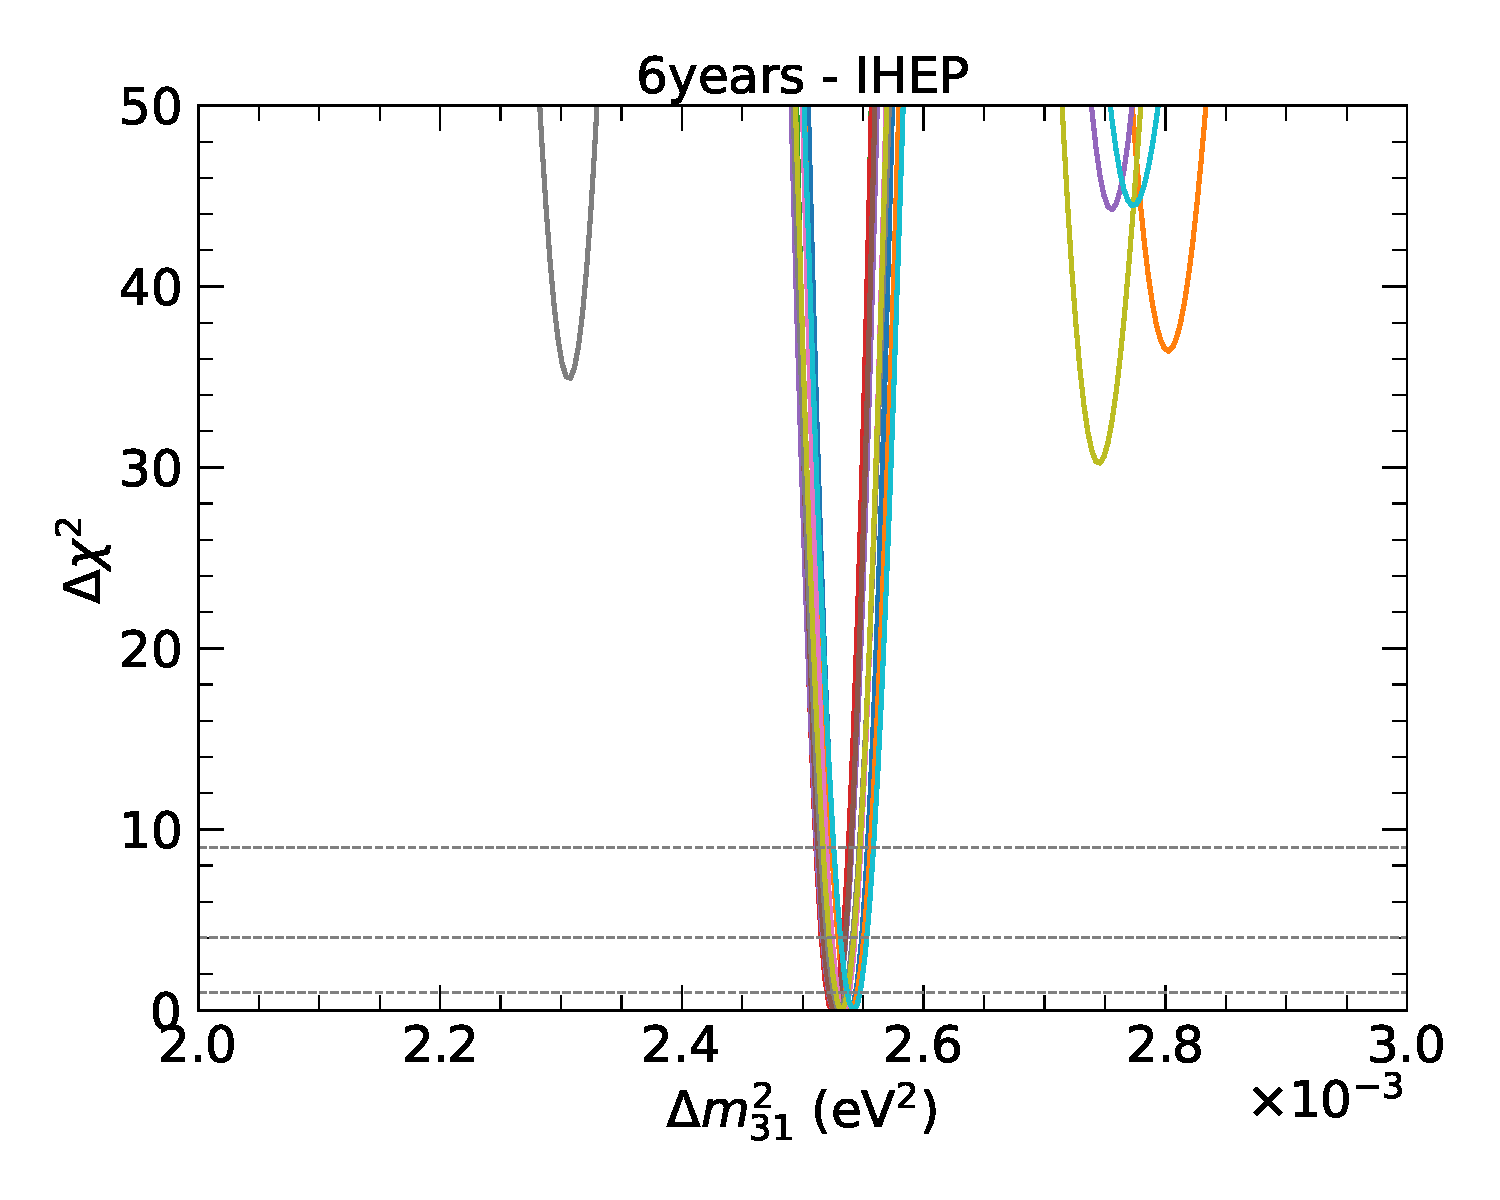
\includegraphics[width=\linewidth]{Img/Jingqin_6years_dmsq31_profile.pdf}
    \caption{6 年统计量}
    \label{fig:dm31_profile_6years}
  \end{subfigure}

  \bicaption[四种统计量下的 $\Delta m^2_{31}$ 侧向轮廓化曲线]{四种统计量下的 $\Delta m^2_{31}$ 侧向轮廓化曲线。}{Profile $\Delta\chi^2$ curves of $\Delta m^2_{31}$ for four different exposures. }
  \label{fig:dm31_profile_exposure}
\end{figure}

图~\ref{fig:dm31_profile_exposure} 展示了四种不同统计量下的 $\Delta m^2_{31}$ 的 $\Delta\chi^2$ 轮廓，可以看到，随着统计量增加，局域极小值和不连续区间出现的概率降低，轮廓趋于单峰和平滑。

\section{Wilks 定理的适用条件与局限}


Wilks 定理为基于对数似然比的检验提供了一条构造置信区间的近似方法。设 $\theta$ 为感兴趣的参数、$\boldsymbol{\eta}$ 为冗余参数（nuisance parameters），定义检验统计量为

\begin{equation}
\lambda_i \;=\; -2\ln\frac{\mathcal{L}(\boldsymbol{x}\mid\theta_i,\hat{\hat{\boldsymbol{\eta}}})}{\mathcal{L}(\boldsymbol{x}\mid\hat\theta,\hat{\boldsymbol{\eta}})}\,,
\end{equation}

其中分子是在参数值 $\theta=\theta_i$ 下，对赘余参数进行条件极大化（以双帽号标注）；分母是对全部参数同时极大化得到的全局极大似然值（以单帽号标注）。Wilks 定理断言：在若干“正则性条件”满足时，上式在大样本极限下渐近服从自由度等于待测参数个数的卡方分布，从而可以直接用卡方分布的分位数作为置信区间构造的阈值（例如 1 自由度时 $\lambda=1,4,9$ 分别对应约 68.27\%、95.45\% 与 99.73\% 的置信水平）\cite{Wilks:1938dza}。

然而，Wilks 近似的成立依赖于若干关键假设 \cite{Wilks:1938dza, Fan:2000gm, Cranmer:2005hi, Cowan:2010js, ParticleDataGroup:2024cfk}，常用的可归纳为：

\begin{itemize}[leftmargin=*,nosep]
  \item \textbf{嵌套假设（nested hypotheses）}：被检验的零假设应当是备择假设的一个特例（在参数估计问题中，检验“参数等于某值”通常满足此条件）。
  \item \textbf{似然函数的光滑性}：对数似然函数在真实参数附近可用二阶泰勒展开（近似为抛物线）、参数位于定义域内部且可导，且极大似然估计值局部唯一。这保证了极大似然估计的渐近正态性与统计量的卡方行为。
  \item \textbf{充分大的样本量}：样本量需足够大以使得上述渐近展开成立并抑制高阶项的影响。
\end{itemize}

在实际问题中，若任一假设被破坏，则 Wilks 近似可能失效。常见导致失效的情形包括：参数位于定义域边界（boundary）处、参数映射导致似然面高度非二次、存在多个不相交的局部极小值（multi-modal likelihood），或样本量过小以致高阶项不可忽略等 \cite{Cowan:2010js, Cranmer:2005hi}。在这些情况下，基于 Wilks 定理的固定 $\Delta\chi^2$ 截值会产生错误的置信区间，通常表现为\textbf{覆盖率偏离名义置信度}（例如发生覆盖率不足，即实际包含真值的概率低于名义置信度）。

对于 JUNO 在早期（低曝光/低统计）阶段对 $\Delta m^2_{31}$ 的测量，上述正则性条件中的若干项被破坏。具体表现为：轮廓化得到的 $\Delta\chi^2$ 曲线在 $\Delta m^2_{31}$ 方向上常常非抛物线、出现多个明显的局部极小值（见第~\ref{sec:2_bad_minima} 节所示轮廓图），这直接违背了局部椭球近似的前提。结果是，按 Wilks 给出的 $\Delta\chi^2=1$ 作为 $1\sigma$ 临界值会低估实际所需的阈值，从而造成对 $\Delta m^2_{31}$ 的置信区间\textbf{欠覆盖}。在我们的模拟覆盖性检验中（详见第 X 节），实证得到的一维经验临界值约为 $\Delta\chi^2_{\mathrm{crit}}\approx1.57$，明显高于 Wilks 近似的 1.0，这正是 Wilks 近似失效的直接证据。

因此，在存在上述非正则情形时，应当放弃直接使用 Wilks 近似给出的固定阈值，而采用基于伪实验（Toy Monte Carlo）的经验方法（例如 Feldman--Cousins 构造）来为每一假设点确定参数依赖的临界 $\Delta\chi^2$，以保证所构造置信区间的频率学覆盖性质正确（详见第 Y 节）\cite{Feldman_1998, Cranmer:2005hi}。


\section{Feldman--Cousins 方法的核心思想}
\label{FC}
基于Wilks定理的局限性，Feldman和Cousins提出了不依赖 Wilks 近似，基于似然比排序原则构建置信区间的方法，通过构造 Neyman 置信带保证正确覆盖率。具体而言，对于任意待检验参数真值 $\delta_i$，通过大量伪实验样本来构建检验统计量（如 $\Delta\chi^2$）的经验分布，然后根据该分布直接确定相应置信度下的临界值 $\Delta\chi^2_{\mathrm{crit}}$。这样，无论统计量分布是否高斯、对称或存在多峰等复杂形状，都能获得恰当的临界 $\Delta\chi^2$，并由此得到正确的置信区间。Feldman 和 Cousins 在原始文献中\cite{Feldman_1998}即以中微子振荡实验为例，验证了该方法可在小信号情形下同时满足正确覆盖率和检验效率。

\section{Feldman--Cousins 方法基本流程}

\begin{itemize}[leftmargin=*,nosep]
  \item \textbf{设定假设真值：}在感兴趣的振荡参数的相关参数空间中，定义一个足够精细的$\delta_i$真值网格，对每个感兴趣的振荡参数真值 $\delta_i$（如 $\Delta m^2_{31}$）作为假设。这里以$\Delta m^2_{31}$为例，定义一个多个点等间距的网格，范围为$[1.5, 3.5]$ eV$^2$。

  \item \textbf{生成伪实验样本：}基于该假设，对于每个假设真值$\delta_i$，生成大量包含统计波动和系统误差的 Toy Monte Carlo 模拟数据。

  \item \textbf{计算检验统计量：}对每个伪数据集执行拟合，得到最优拟合 $\chi^2$ 值，并利用公式~\ref{eq:lambda_ij_FC_chi2}计算检验统计量 $\Delta\chi^2(\delta_i)$。
  \begin{equation}\label{eq:lambda_ij_FC_chi2}
    \Delta\chi^2(\delta_i) = \chi^2(x_{ij}\mid\delta_i) - \chi^2(x_{ij}\mid\hat{\delta}_j)
\end{equation}

    其中，$\chi^2(x_{ij}\mid\delta_i)$ 表示在固定参数取值 $\delta_i$ 时，对该 toy 的所有冗余参数进行轮廓化后得到的 $\chi^2$ 轮廓；$\chi^2(x_{ij}\mid\hat{\delta}_j)$ 则表示在全局最小点处评估的 $\chi^2$ 轮廓，其中 $(\hat{\delta}_j)$ 代表对所有参数同时拟合得到的全局最佳拟合值。

    \item \textbf{确定临界值：}基于所有伪实验，按照 Feldman--Cousins 排序规则，得到 $\Delta\chi^2(\delta_i)$ 的经验分布。见式~\ref{eq:FC_integral}，在给定置信度（如 68.27\%）下可以确定临界值 $\Delta\chi^2_{\mathrm{crit}}(\delta_i)$，置信区间即由满足 $\Delta\chi^2 \le \Delta\chi^2_{\mathrm{crit}}(\delta_i)$ 的 $\delta_i$ 组成。
    \begin{equation}
        \int_0^{\Delta\chi^{2,\alpha}_{\mathrm{crit}}(\delta_i)} P\!\left(\Delta\chi^2(\delta_i, \delta_{\mathrm{bft}})\right)\,\mathrm{d}(\Delta\chi^2) = 1-\alpha \;\longleftrightarrow\; \Delta\chi^{2,\alpha}_{\mathrm{crit}}(\delta_i)
        \label{eq:FC_integral}
    \end{equation}
\end{itemize}

上述步骤使用 Toy MC 确定的临界 $\Delta\chi^2$ 取代了 Wilks 定理给出的固定值，从而保证了置信区间的实际覆盖率。该流程确保了即便统计分布偏离高斯、或出现多解时，所得的置信区间仍然是可靠的。

\section{Feldman--Cousins 覆盖性研究}  
为了在非正则情形下验证 Wilks 定理的适用性并获得具有正确频率学覆盖率的置信区间，我们对若干目标振荡参数进行了 Feldman--Cousins（FC）覆盖性研究。研究包括对太阳振荡参数的二维 FC 构造，以及对 $\Delta m^2_{31}$ 的一维 FC 构造。

\subsection{对 $\Delta m^2_{21}$ 与 $\sin^2\theta_{12}$ 的二维 Feldman--Cousins}  
为了评估各个振荡参数的覆盖率特性，我们基于前述的 Feldman--Cousins 的标准步骤，通过在名义假设下生成大量伪实验（toys），并对每个伪实验重新拟合来构造检验统计量
\begin{equation}
  \Delta\chi^2(\delta)\equiv \chi^2(\delta)-\chi^2_{\min}
\end{equation}
的经验分布。
如图X.X所示，来自伪实验的参数联合分布显示 $\Delta m^2_{21}$ 与 $\sin^2\theta_{12}$ 之间存在明显的相互关联（在本示例的 toy 样本中，两者的皮尔逊相关系数约为 $-0.29$），因此在评估这两个太阳区振荡参数的覆盖性质时应采用二维的 Feldman–Cousins 构造，以保证置信区间在参数关联存在时仍然具有正确的覆盖率。
对于二维参数空间 $(\Delta m^2_{21},\,\sin^2\theta_{12})$，渐近情形下检验统计量应服从自由度为 2 的 $\chi^2$ 分布。

\begin{figure}[htbp]
    \centering
    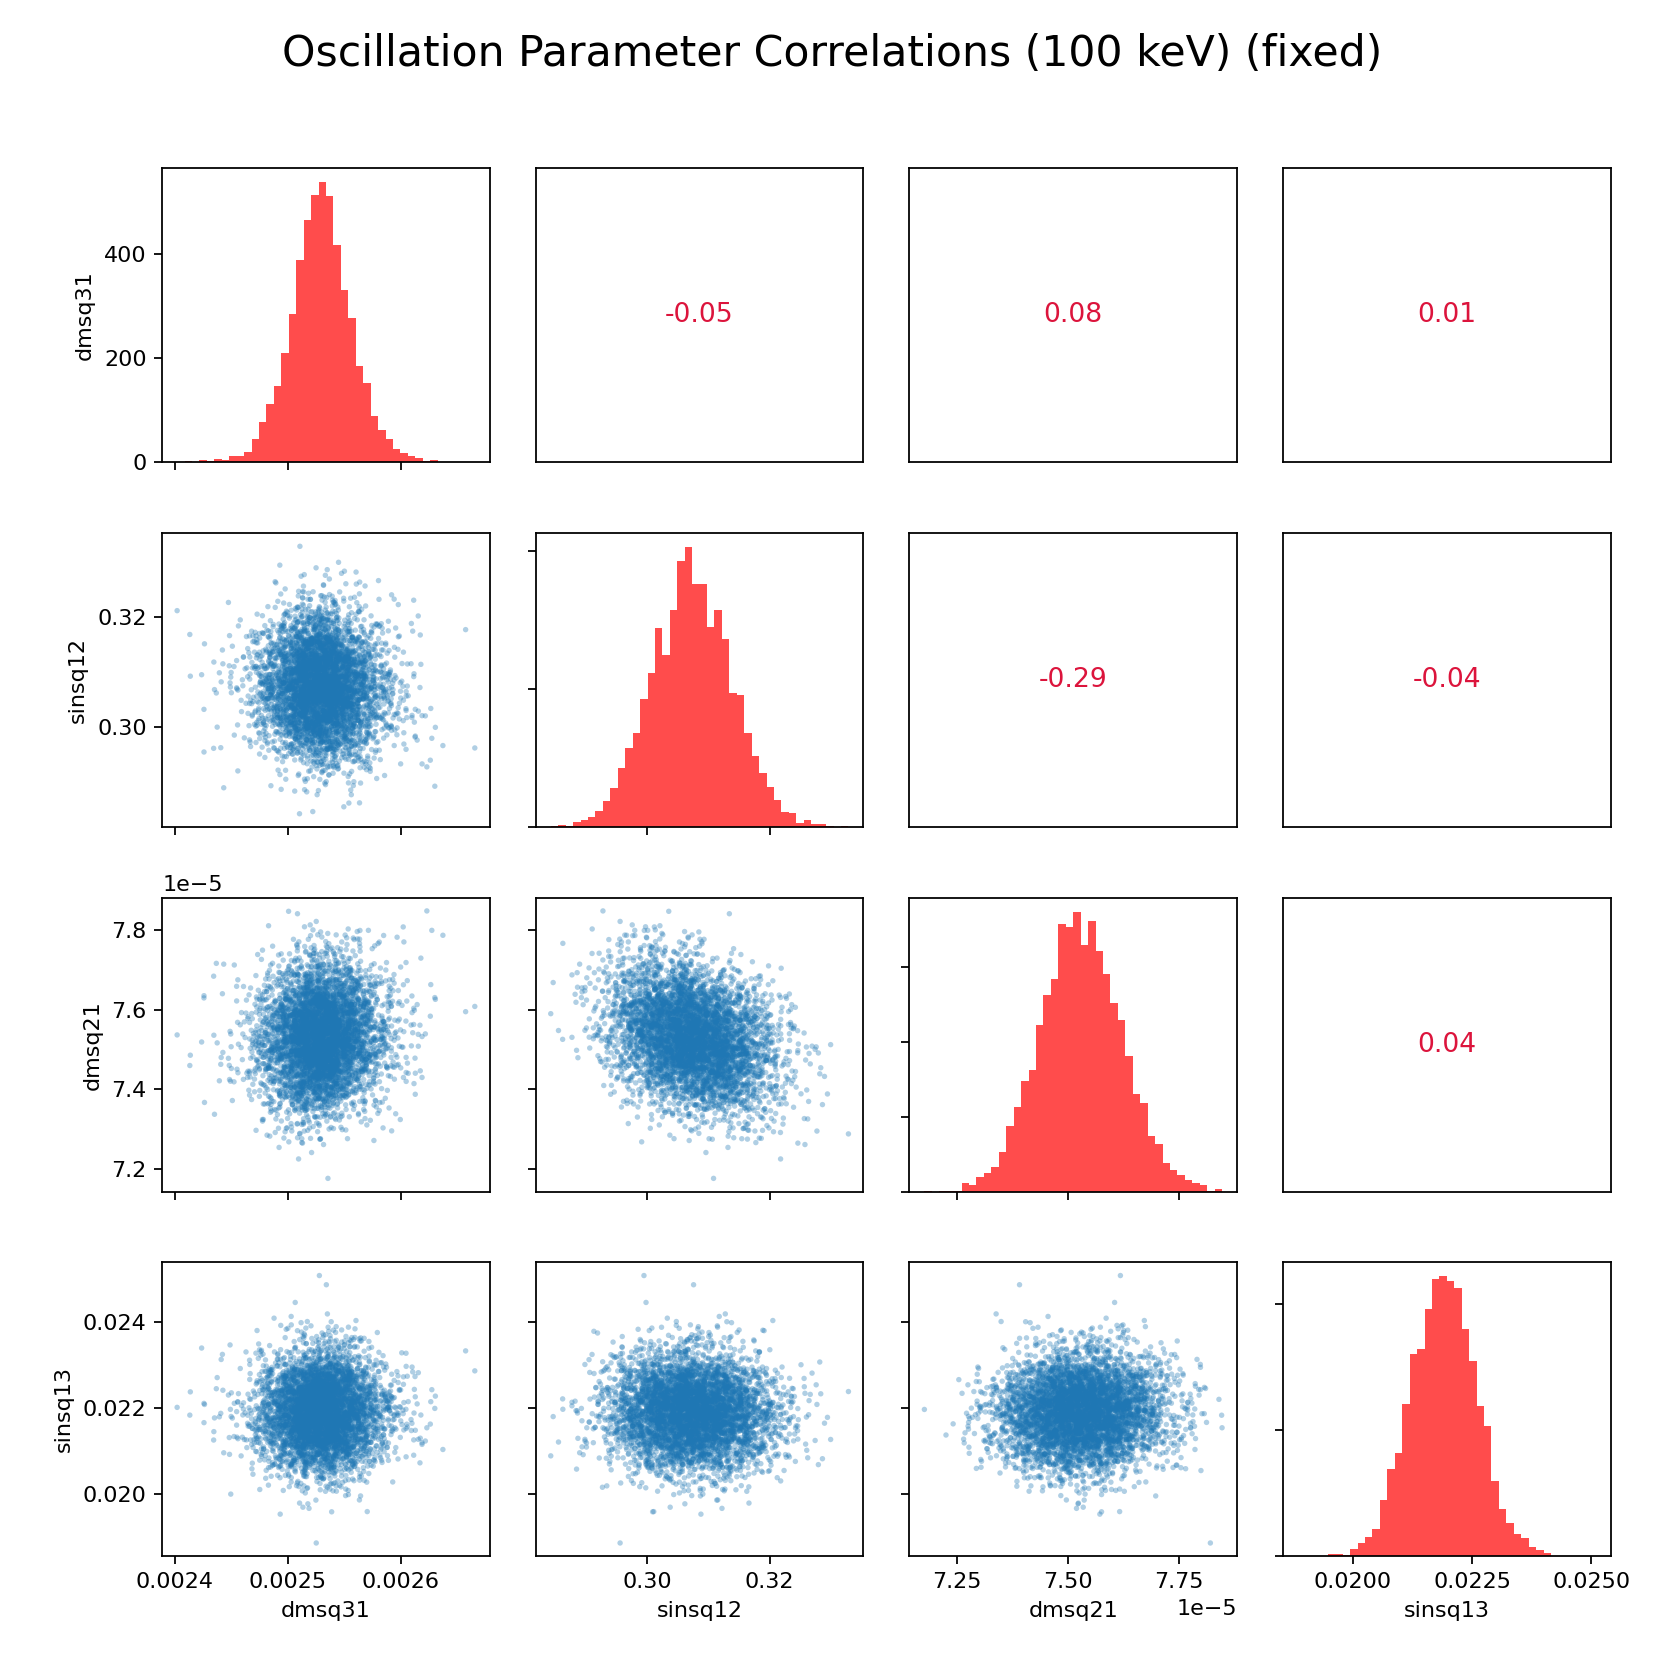
\includegraphics[width=0.75\textwidth]{Img/dmsq21_sinsq12.png}
    \bicaption{振荡参数的两两关联与边缘分布（反应堆中微子能量分段 100 keV，固定反应堆模型）。对角线为每个参数的边缘直方图；下三角为参数间散点图；上三角数值为对应的皮尔逊相关系数（图中 $\Delta m^2_{21}$ 与 $\sin^2\theta_{12}$ 的相关系数约为 $-0.29$）。这些关联说明在构造置信区间时需要考虑参数间的耦合，因此对太阳区参数采用二维 FC 构造更为合适。}{Pairwise correlations and marginal distributions of the oscillation parameters (reactor neutrino energy binning 100 keV, fixed reactor model). Diagonal panels show marginal histograms for each parameter; lower-triangular panels show pairwise scatter plots; upper-triangular entries report the corresponding Pearson correlation coefficients (the correlation between $\Delta m^2_{21}$ and $\sin^2\theta_{12}$ is about $-0.29$). These correlations motivate the use of a 2D Feldman–Cousins construction for the solar-sector parameters to properly account for their coupling when producing confidence intervals.}
    \label{fig:osc_param_corr}
  \end{figure}

图~\ref{fig:FC21} 给出在参数平面中某代表性格点处得到的经验 $\Delta\chi^2$ 分布。提取到的 68.27\% 置信水平下的临界值在统计不确定度范围内与 Wilks 期望值一致（$\chi^2(ndf = 1)$，1$\sigma$的临界值$\Delta\chi^2 \approx  2.3$）。因此，对于太阳区参量 $(\Delta m^2_{21},\sin^2\theta_{12})$，在所测试的参数区间内，Wilks 近似是充足的，可以用常规定义的卡方临界值来构造置信域。

\begin{figure}[h]
  \centering
  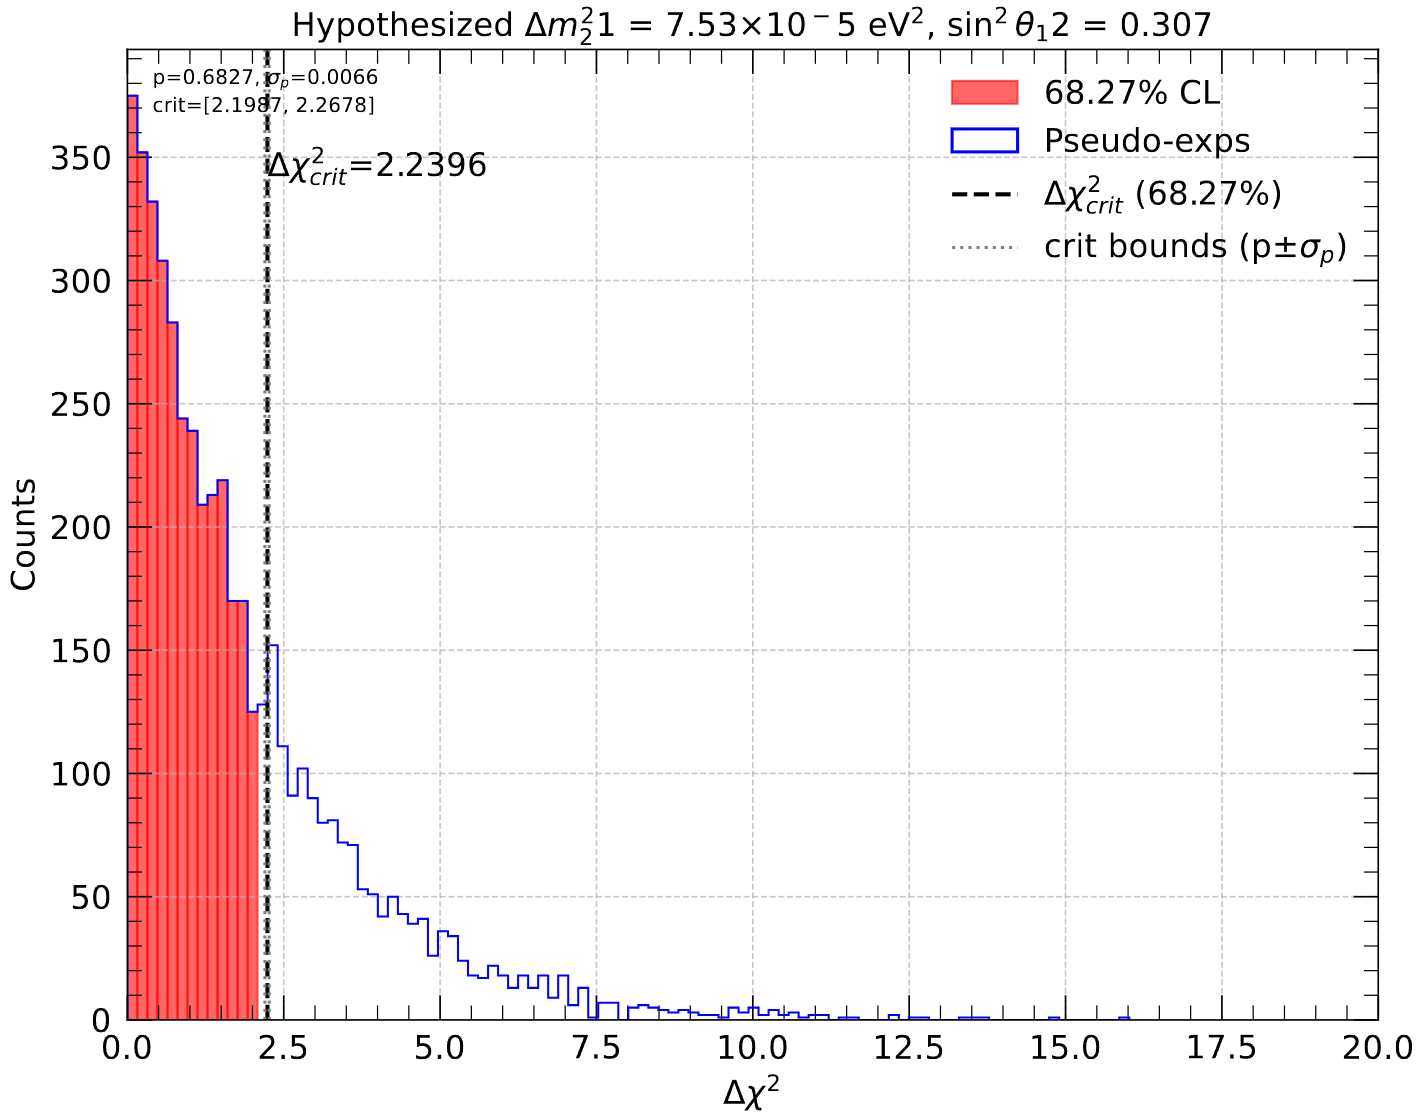
\includegraphics[width=0.7\linewidth]{Img/FC21.png}
  \bicaption[50天统计量下，二维 Feldman--Cousins 检验的经验 $\Delta\chi^2$ 分布]
  {来自二维 Feldman--Cousins 检验（在 $(\Delta m^2_{21},\,\sin^2\theta_{12})$ 参数平面某代表点处）的经验 $\Delta\chi^2$ 分布。虚线竖线指示 68.27\% 置信水平下的临界值，结果与自由度为 2 的 Wilks 期望相符。}
  {Empirical $\Delta\chi^2$ distribution from the 2D Feldman--Cousins test at a representative point in the $(\Delta m^2_{21},\,\sin^2\theta_{12})$ parameter space. The vertical dashed line indicates the critical value at 68.27\% C.L., which agrees with the Wilks expectation of a two-degrees-of-freedom $\chi^2$ distribution.}
  \label{fig:FC21}
\end{figure}

\subsection{对 $\Delta m^2_{31}$ 的一维 Feldman--Cousins}  
相比之下，$\Delta m^2_{31}$ 的似然面表现出非正则行为（附近存在非物理的低值极小与相位简并效应），这使得在纯 JUNO 配置下直接使用 Wilks 近似不再可靠。因此我们对 $\Delta m^2_{31}$ 采用一维 FC 构造。为评估反应堆谱模型依赖的影响，FC 构造分两步进行：

\begin{enumerate}  
\item \textbf{固定反应堆模型：} 设反应堆谱固定为平均 Summation Model（不做谱形扰动），在该条件下生成伪实验样本并计算经验 $\Delta\chi^2$ 分布。得到的 68.27\% 接受域临界值为
\[
 \Delta\chi^2_{\rm crit,\,fixed} = 1.5379,
\]
对应 50 天曝光下 $\Delta m^2_{31}$ 的测量精度为 $1.39\%$。该固定模型下每个 toy 的精度分布如图~\ref{fig:dmsq31_fixedaveSM} 所示。  
\item \textbf{变化反应堆模型（包含谱形扰动）：} 为了包含反应堆模型的变化，我们通过对每个 20 keV 段进行扰动（构造出一族带有精细结构的替代谱），抽样生成一组被扰动的反应堆谱（采样模型集合，$N_{\rm toys}=5000$），并在这些扰动模型上重复 FC 构造。此时经验临界值变为
\[
 \Delta\chi^2_{\rm crit,\,sampled} = 1.5724,
\]
对应的 $\Delta m^2_{31}$ 精度为 $1.40\%$（50 天曝光）。采样（高斯扰动）模型下的每个 toy 精度分布见图~\ref{fig:dmsq31_gaussian}。  
\end{enumerate}

\begin{figure}[htbp]
  \centering
  \begin{subfigure}[t]{0.47\textwidth}
    \centering
    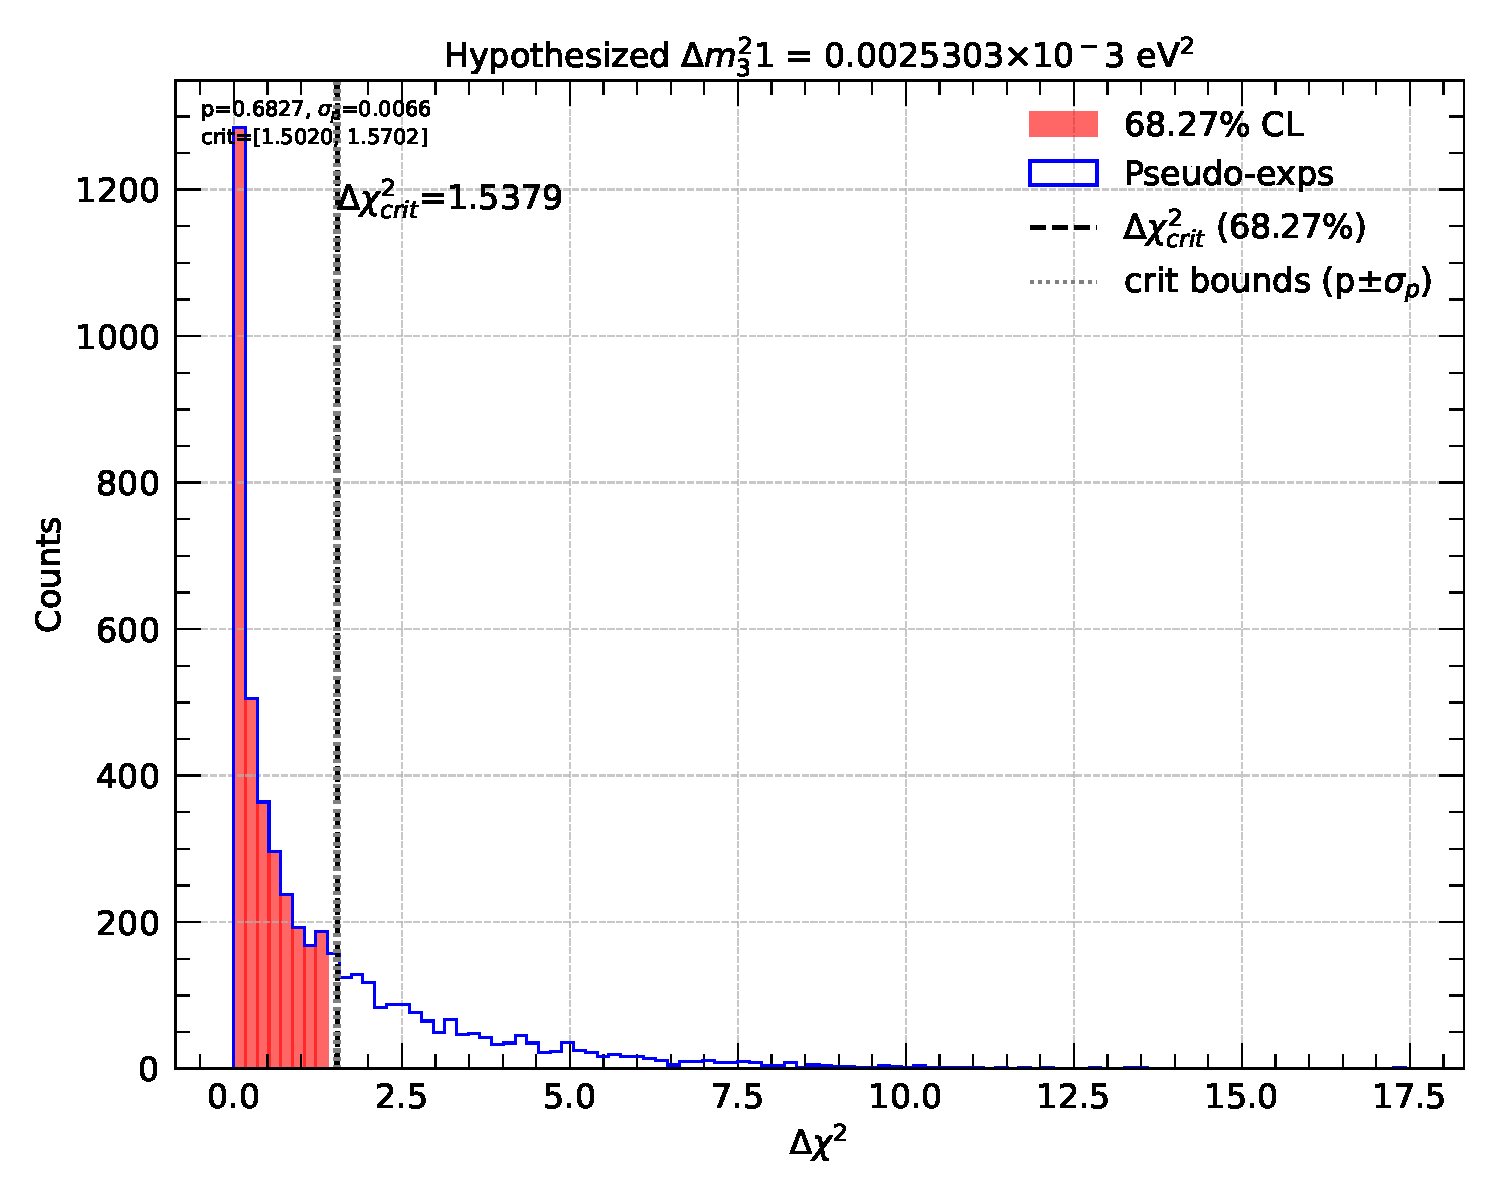
\includegraphics[width=\linewidth]{Img/segment_300_rec_100_0_0025303_dmsq31_constraint_dchi2.pdf}
    \caption{固定反应堆模型}
    \label{fig:fc_dchi2_fixed}
  \end{subfigure}
  \hfill
  \begin{subfigure}[t]{0.47\textwidth}
    \centering
    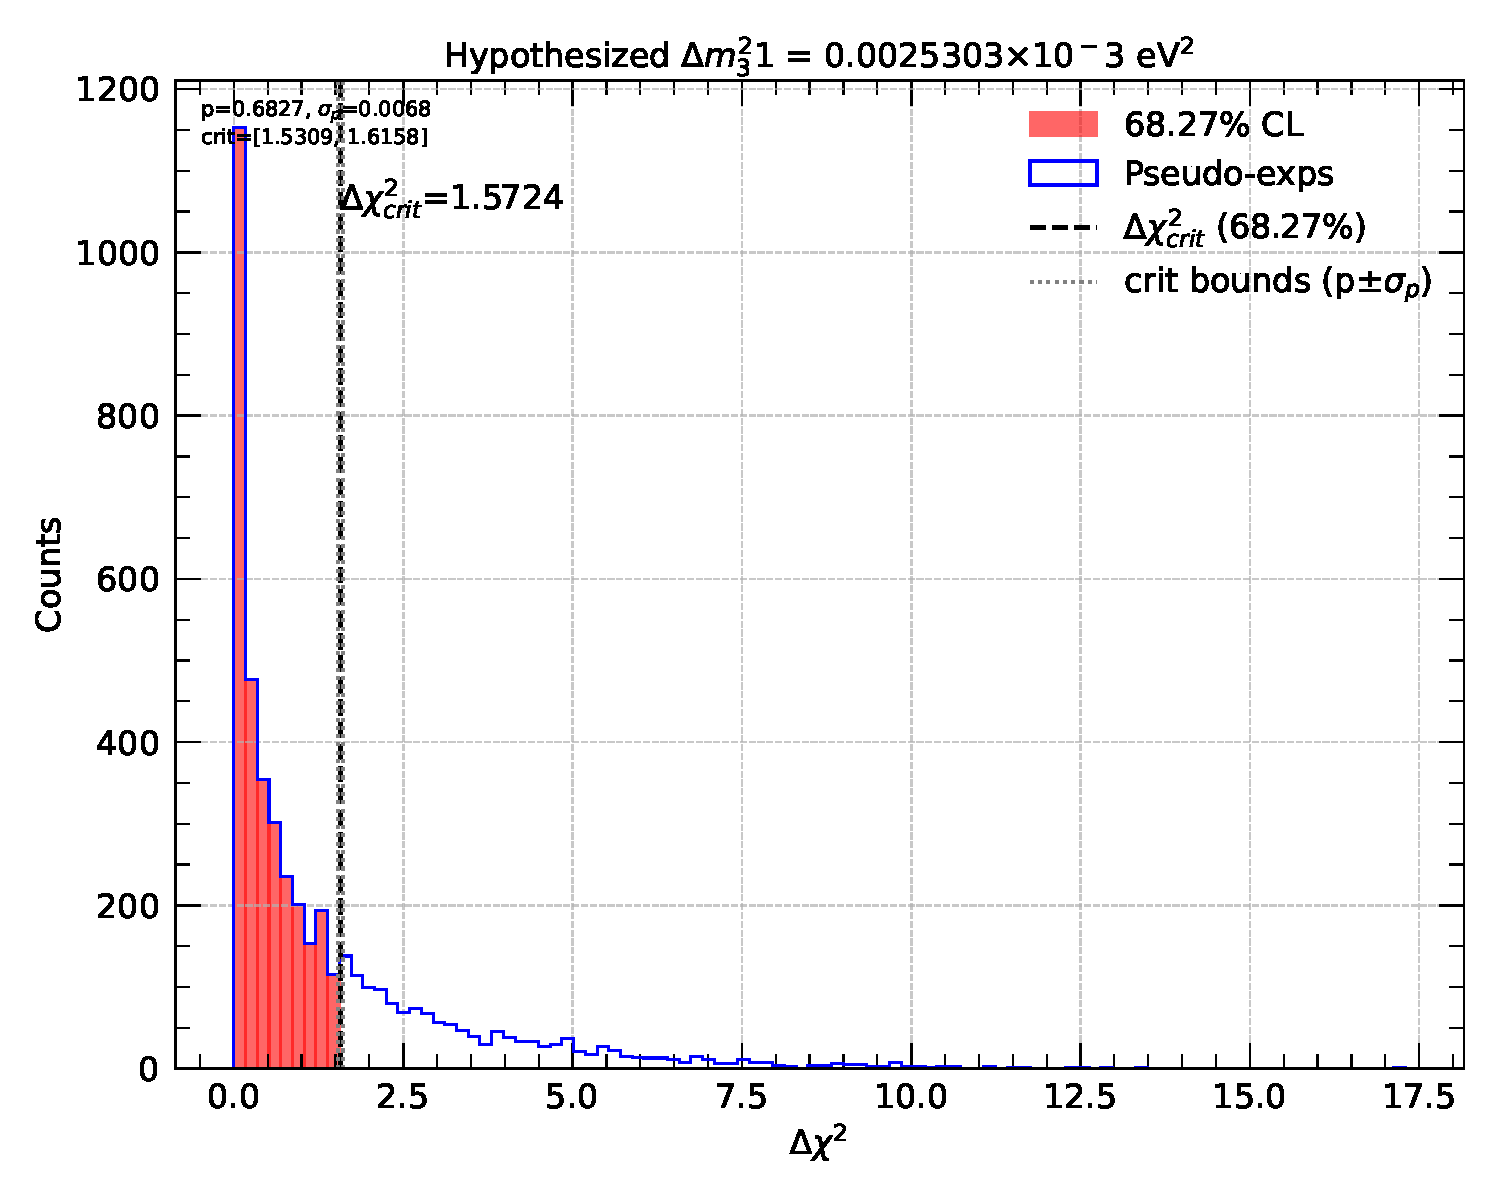
\includegraphics[width=\linewidth]{Img/segment_300_rec_100_0_0025303_dmsq31_constraint_dchi2_vary.pdf}
    \caption{变化反应堆模型}
    \label{fig:fc_dchi2_sampled}
  \end{subfigure}

  \bicaption[四种统计量下的 $\Delta m^2_{31}$ 侧向轮廓化曲线]{基于 Feldman–Cousins 构造得到的经验检验统计量 $\Delta\chi^2$ 分布（50 天统计量）。左图：固定反应堆模型下的结果；红色柱状表示被接受到 68.27\% 接受域内的伪实验（填充），蓝色轮廓为所有伪实验的分布（pseudo-exps）；虚线表示对应于 68.27\% 的经验临界值 $\Delta\chi^2_{\rm crit}=1.5379$。右面板：在扰动（sampled）反应堆模型（包含谱形细结构扰动）下的结果；对应经验临界值为 $\Delta\chi^2_{\rm crit}=1.5724$。两幅图均使用相同的横轴与归一化方式，展示了模型不确定性对经验临界值的微小影响。}
  {Empirical distributions of the test statistic $\Delta\chi^2$ obtained with the Feldman–Cousins construction (50-day exposure). Left panel: fixed reactor-model case; the red filled histogram shows the toys accepted within the 68.27\% acceptance region, while the blue outline shows the full pseudo-experiment distribution; the vertical dashed line marks the empirical critical value $\Delta\chi^2_{\rm crit}=1.5379$ (68.27\%). Right panel: sampled/perturbed reactor-model ensemble (including fine-structure perturbations); the empirical critical value in this case is $\Delta\chi^2_{\rm crit}=1.5724$. Both panels use identical axis scaling and normalization and illustrate the (small) effect of reactor-model variation on the FC-derived critical value.}
  \label{fig:dmsq31_FC_histograms}
  \label{fig:fc_dchi2_fixed_vs_sampled}
\end{figure}

当采用采样的反应堆模型集合时，经验临界值较固定模型略有上升，但差别较小；且通过增加 FC 中的伪实验数量可以进一步降低经验临界值的统计不确定性。

由上述研究可得出以下结论：  
\begin{itemize}  
\item 反应堆模型变化对 $\Delta m^2_{31}$ 的附加系统贡献很小：在 50 天情形下估计该项对 $\Delta m^2_{31}$ 精度的影响小于 $0.3\%$。  
\item 对三项参数（$\Delta m^2_{21}$, $\sin^2\theta_{12}$, $\Delta m^2_{31}$）而言，在 50 天曝光下由现实可行的反应堆模型变化引入的系统不确定度均小于统计不确定度；即在该曝光下模型相关系统误差可视为次要。  
\item 在所采用的假设下，基于 FC 的 $\Delta m^2_{31}$ 精度约为 $1.4\%$（50 天），略差于全局拟合给出的约 $1.1\%$ 的精度，但在仅用 JUNO 数据并考虑反应堆模型不确定性的内部一致性下该结果是合理的。  
\end{itemize}

\paragraph{实践说明}  
上述 FC 结果中，采样模型情形使用了 $N_{\rm toys}=5000$ 个伪实验；增大 $N_{\rm toys}$ 能降低经验临界值的统计不确定性，因此上述数值应当带有伪实验统计误差的说明。

\begin{figure}[!htbp]  
\centering  
\begin{subfigure}[t]{0.45\textwidth}  
\centering  
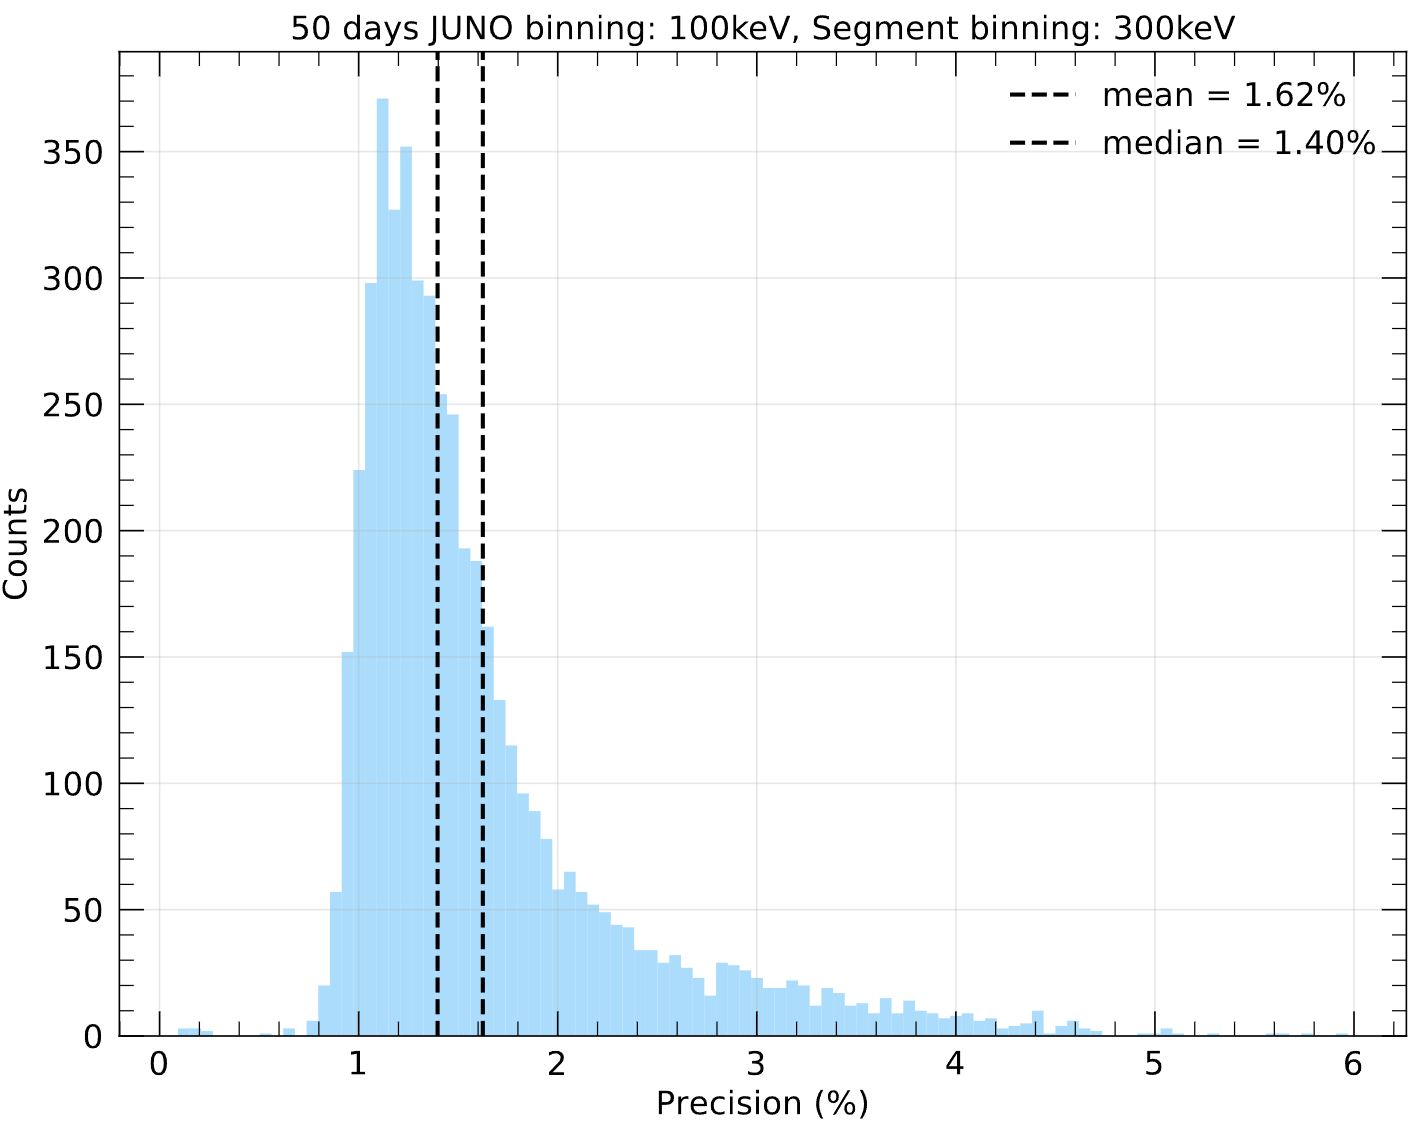
\includegraphics[width=\linewidth]{Img/dmsq31_gaussian.png}  
\bicaption{采样（高斯扰动）反应堆模型集合下的每个 toy 精度分布（$N_{\rm toys}=5000$）。}{Per-toy precision distribution for the sampled (Gaussian-perturbed) reactor-model ensemble ($N_{\rm toys}=5000$).}  
\label{fig:dmsq31_gaussian}  
\end{subfigure}%  
\hfill  
\begin{subfigure}[t]{0.45\textwidth}  
\centering  
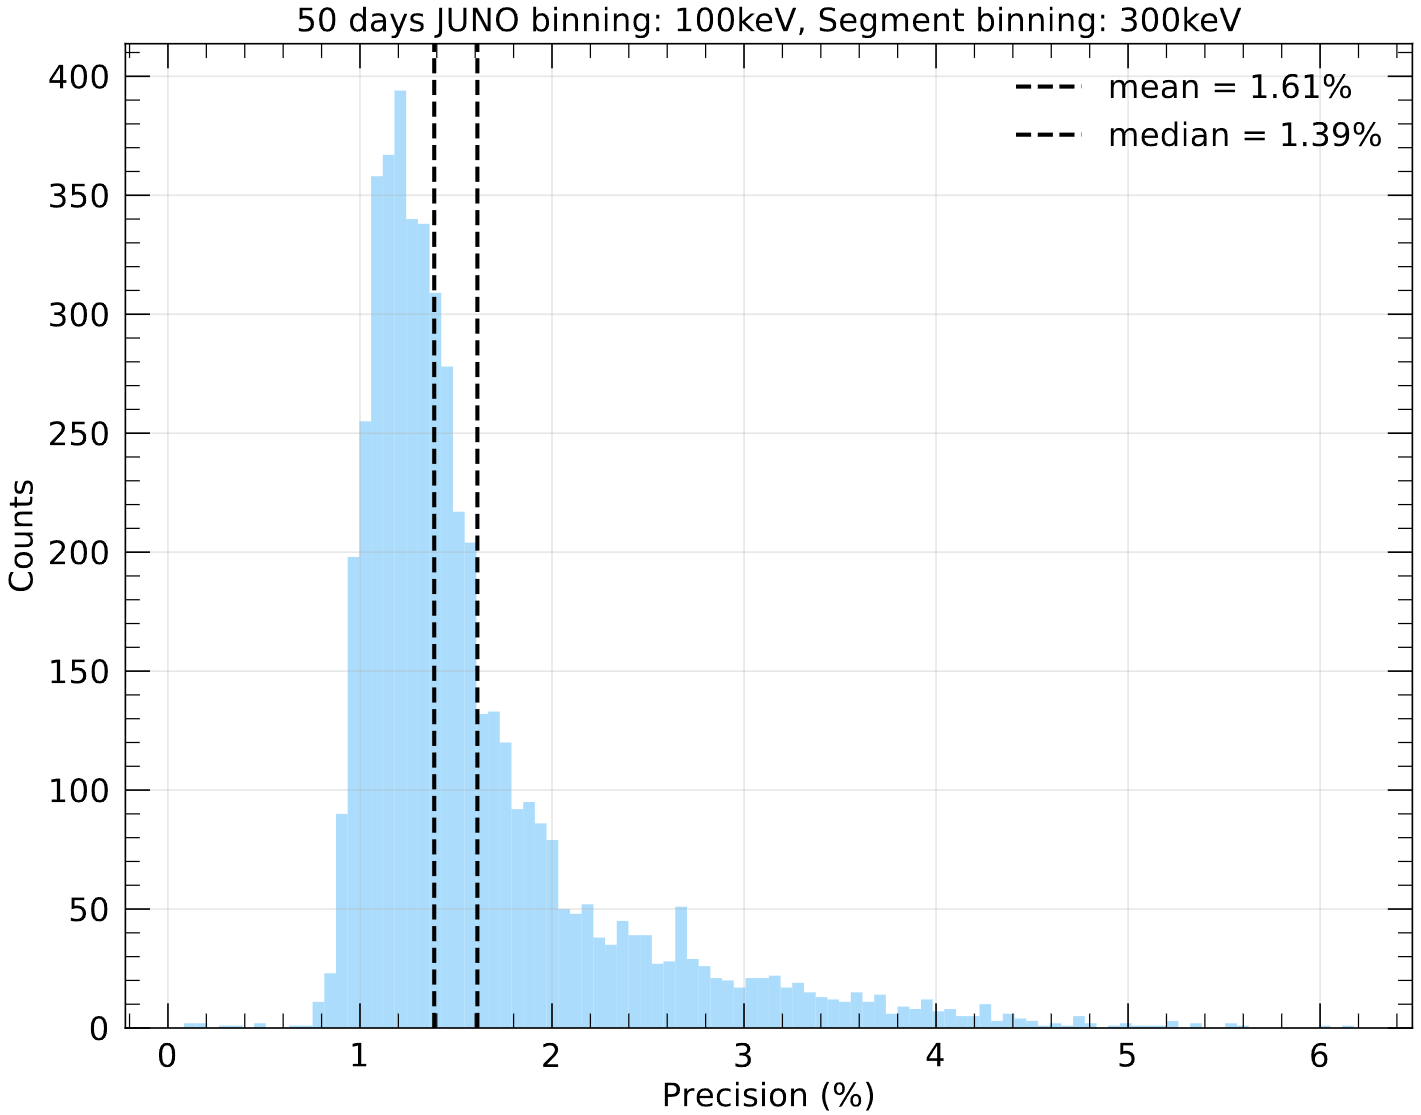
\includegraphics[width=\linewidth]{Img/dmsq31_fixedaveSM.png}  
\bicaption{固定平均 Summation Model（无谱形扰动）情形下的每个 toy 精度分布（$N_{\rm toys}=5000$）。}{Per-toy precision distribution for the fixed average Summation Model ($N_{\rm toys}=5000$) (no shape perturbation).}  
\label{fig:dmsq31_fixedaveSM}  
\end{subfigure}  
\caption{用于评估 $\Delta m^2_{31}$ 精度与模型敏感性的 per-toy 精度分布比较（左：采样模型；右：固定模型）。}  
\label{fig:dmsq31_FC}  
\end{figure}

\section{在振荡参数上的应用}

\begin{itemize}
    \item acceptance intervals；
    \item significance profiles；
    \item 自由/固定拟合。
\end{itemize}

\section{$\Delta m^2_{31}$的复杂性：多局域极小与不连续置信区间}
\begin{itemize}
    \item 小振荡结构与谱型耦合导致似然多峰（简并）
    \item toy生成策略(含不同反应堆谱假设、背景波动、响应扰动等）
    \item 基于toyMC的$\Delta m^2_{31}$灵敏度研究方法
    \item toy 拟合流程、多峰计数与区间形态统计（单区间比率 vs 多区间出现概率）
    \item 结果展示：多局域极小的分布、区间宽度与覆盖率的影响
    \item 对实验结果解读的影响（JUNO 早期数据如何报告 $\Delta m^2_{31}$的策略建议）    
\end{itemize}


\section{Toy MC 生成与统计处理}

\begin{itemize}
    \item 系统误差纳入 toy；
    \item $\Delta\chi^2$ 样本与分位点。
\end{itemize}

\section{Corrected intervals 与覆盖率验证}

\begin{itemize}
    \item corrected critical $\chi^2$；
    \item 覆盖率检验。
\end{itemize}

\section{IHEP cluster上的高性能实现}

\begin{itemize}
    \item 调度、并行颗粒度；
    \item 失败重试；
    \item 性能数据。
\end{itemize}

\section{Feldman--Cousins 最终结果展示}

\begin{itemize}
    \item FC 置信区间（2D contour）；
    \item 与 Wilks/Asimov 的比较；
    \item 对 $\sin^2\theta_{12}$、$\Delta m^2_{21}$ 的影响。
\end{itemize}

%=====================================================================
\chapter{结果与讨论（Results \& Discussion）}
%=====================================================================

\section{加速效果总结}

\begin{itemize}
    \item speed-up、CPU-hours 节省；
    \item 误差相容性。
\end{itemize}

\section{物理结果与不确定性}

\begin{itemize}
    \item JUNO+DYB 拟合结果；
    \item FC 与 Wilks 对比。
\end{itemize}

\section{方法局限性}

\begin{itemize}
    \item GP 不确定度；
    \item 拟合失败、多模态；
    \item I/O 瓶颈。
\end{itemize}

\section{对未来实验与分析的建议}

\begin{itemize}
    \item GPU 加速；
    \item 更稳定的最小化策略；
    \item ML surrogate 深化；
    \item 开放数据与工具。
\end{itemize}

%=====================================================================
\chapter{结论与展望（Conclusions \& Outlook）}
%=====================================================================

\begin{itemize}
    \item 总结主要贡献（加速倍数、覆盖率保持等关键数字）；
    \item 展望：GP 在线扫描、拓展到 DUNE/TAO、异构计算等方向。
\end{itemize}

